\documentclass[a4paper,12pt,twoside]{report}
\usepackage[left=2.5cm,right=2.5cm,top=2cm,bottom=2.5cm]{geometry}

% Paquete para el manejo de títulos y secciones
\usepackage{titlesec}
\usepackage[spanish, es-tabla]{babel}
\usepackage[utf8]{inputenc}
\selectlanguage{spanish} 
\usepackage[T1]{fontenc}
\usepackage{fancyhdr}

\decimalpoint

% Paquetes para la inclusión de gráficos, tablas y figuras
\usepackage{caption} 
\captionsetup[figure]{labelfont=bf, textfont=normalfont}
\captionsetup[table]{labelfont=bf, textfont=normalfont}
\usepackage{graphicx}
\usepackage[table]{xcolor}
\usepackage{multirow}
\usepackage{subcaption}
\usepackage{float}
\usepackage{pbox}
\usepackage{adjustbox}

\usepackage{verbatim}
\setlength{\headheight}{30pt}
\addtolength{\topmargin}{-15pt}

% Paquetes para algoritmos y pseudocódigo
\usepackage{algpseudocode}
\usepackage{algorithm}    
\input{spanishAlgorithmic}

% Paquetes para tipografía y estilo visual
\usepackage{microtype} 
\usepackage{textcomp}
\usepackage{gensymb}
\usepackage{amsfonts}
\usepackage{amsthm}
\usepackage{amsmath, amssymb}
\usepackage{bm}
\usepackage{setspace}
% \usepackage{upgreek}  % No disponible en TinyTeX - no se usa
% \usepackage{units}    % No disponible en TinyTeX - no se usa
% \usepackage{nccmath}  % No disponible en TinyTeX - no se usa

% Paquetes para tablas avanzadas
\usepackage{booktabs, array, tabularx, longtable}
\usepackage{enumitem}

% Paquetes para código y listings
\usepackage{listings}
\usepackage{newfloat}
\usepackage{courier}
\usepackage[header,title]{appendix}

% --- Paleta Nord (https://nordtheme.com) ---
\definecolor{nordDark}{HTML}{2E3440}        % Polar Night  — texto, bordes
\definecolor{nordGray}{HTML}{4C566A}        % Polar Night 3 — bordes medios
\definecolor{nordSnow}{HTML}{ECEFF4}        % Snow Storm   — fondos
\definecolor{nordFrost}{HTML}{5E81AC}       % Frost Blue   — acentos
\definecolor{nordGreen}{HTML}{A3BE8C}       % Aurora Green — régimen estable
\definecolor{nordYellow}{HTML}{EBCB8B}      % Aurora Yellow — régimen moderado
\definecolor{nordRed}{HTML}{BF616A}         % Aurora Red   — régimen caída
% --- Colores heredados (portada, listings) ---
\definecolor{mygold}{RGB}{244,190,2}
\definecolor{myblue}{HTML}{003E6F}
\definecolor{mygray}{RGB}{128,128,128}

% --- Configuración de Listings para Código ---
\newfloat{listing}{H}{lol}
\floatname{listing}{Código}
\renewcommand{\lstlistingname}{Código}
\renewcommand{\lstlistlistingname}{Lista de Códigos}
\lstset{
  inputencoding=utf8,
  literate={á}{{'a}}1 {é}{{'e}}1 {í}{{'i}}1 {ó}{{'o}}1 {ú}{{'u}}1 {ñ}{{\~n}}1 {Ó}{{'O}}1,
  basicstyle=\ttfamily\footnotesize,
  keywordstyle=\color{myblue},
  numberstyle=\tiny\color{mygray},
  numbers=left,
  stepnumber=1,
  numbersep=5pt,
  backgroundcolor=\color{white},
  showstringspaces=false,
  frame=single,
  rulecolor=\color{black},
  tabsize=4,
  captionpos=b,
  breaklines=true,
  breakatwhitespace=false
}
\lstnewenvironment{python}[1][]{\lstset{language=Python, #1}}{}
\lstnewenvironment{consola}[1][]{\lstset{basicstyle=\ttfamily\footnotesize\color{mygray}, #1}}{}

% Paquetes para TikZ y PGFPlots
\usepackage{tikz}
\usepackage{pgfplots}
\pgfplotsset{compat=1.18}
\usetikzlibrary{automata, positioning, arrows.meta, fit, matrix, decorations.pathmorphing, shapes.geometric, babel, shadows, calc}
\shorthandoff{>}\shorthandoff{<}

% Paquetes para manejo de índices y listados
\usepackage[intoc,spanish]{nomencl}
\usepackage{color}
\newcommand{\source}[1]{\caption*{Fuente: {#1}} }
\usepackage{lscape}
\floatstyle{plaintop}

% Paquetes para citas y bibliografía
\usepackage[numbers,sort&compress]{natbib}
\usepackage[hidelinks]{hyperref}
\hypersetup{
    colorlinks=true,
    linkcolor=black,
    citecolor=myblue,
    urlcolor=myblue,
    pdfauthor={Norman Reynaldo Sabillon Castro},
    pdftitle={Modelado de Series Temporales Económicas},
    pdfsubject={Tesis de Maestría en Matemáticas},
    pdfkeywords={TCROC, series temporales, economía, finanzas, K-Means, NNLS}
}

\newcommand\scalemath[2]{\scalebox{#1}{\mbox{\ensuremath{\displaystyle #2}}}}
\newcommand{\eqdef}{\mathrel{\overset{\mathrm{def}}{=}}}     % símbolo :=


\setcounter{tocdepth}{3}
\setcounter{secnumdepth}{3}

% ===================================================================
%   COMANDOS MATEMÁTICOS Y ENTORNOS PERSONALIZADOS
% ===================================================================
\DeclareMathOperator*{\argmin}{arg\,min}
\DeclareMathOperator{\diag}{diag}
\DeclareMathOperator{\tr}{tr}

\newcommand{\mat}[1]{\mathbf{#1}}
\newcommand{\vect}[1]{\mathbf{#1}}
\newcommand{\set}[1]{\mathcal{#1}}
\newcommand{\supermat}[1]{\mathbb{#1}}
\newcommand{\R}{\mathbb{R}}
\newcommand{\N}{\mathbb{N}}
\newcommand{\E}{\mathbb{E}}
\newcommand{\Cov}{\text{Cov}}
\newcommand{\Var}{\text{Var}}

% --- Entornos tipo Teorema (Numerados por capítulo) ---
\theoremstyle{plain}
\newtheorem{theorem}{Teorema}[chapter]
\newtheorem{lemma}[theorem]{Lema}
\newtheorem{proposition}[theorem]{Proposición}
\newtheorem{corollary}[theorem]{Corolario}
\newtheorem{property}[theorem]{Propiedad}

\theoremstyle{definition}
\newtheorem{definition}{Definición}[chapter]
\newtheorem{examplex}{Ejemplo}[chapter]
\newtheorem{assumption}{Suposición}[chapter]

\theoremstyle{remark}
\newtheorem*{remark}{Observación}

% Paquete para referencias automáticas
\usepackage[nameinlink]{cleveref}
\Crefname{figure}{Figura}{Figuras}
\Crefname{table}{Tabla}{Tablas}
\Crefname{equation}{Ecuación}{Ecuaciones}
\newcommand\crefrangeconjunction{--}

% Definición de fracciones
\newcommand{\ffrac}[2]{\ensuremath{\frac{\displaystyle #1}{\displaystyle #2}}}

% Configuración de títulos de capítulos
\titleformat{\chapter}[display]
{\normalfont\Huge\bfseries}{\chaptertitlename\ \thechapter}{20pt}{\LARGE}
\titlespacing*{\chapter}{0pt}{-30pt}{0pt}

\usepackage{etoolbox}
% \AtBeginEnvironment{align*}{\useshortskip}  % Requiere nccmath
% \AtBeginEnvironment{align}{\useshortskip}   % Requiere nccmath

\makeatletter

\newbox\namebox
\newdimen\signboxdim

\def\signature#1{%
    \setbox\namebox=\hbox{#1}
    \signboxdim=\dimexpr(\wd\namebox+2cm)
    \parbox[t]{\signboxdim}{%
        \centering
            \hrulefill\\    % for a line
            #1
        \par}%
    }
\if@titlepage

\renewcommand\maketitle{
    \begin{titlepage}%

   \begin{center}

\textbf{UNIVERSIDAD NACIONAL AUTÓNOMA DE HONDURAS}\\
\textbf{FACULTAD DE CIENCIAS}\\
\textbf{ESCUELA DE MATEMÁTICA Y CIENCIAS DE LA COMPUTACIÓN}\\
\textbf{MAESTR\'IA EN MATEMÁTICA}
\end{center}

\begin{figure}[H]
\centering

\includegraphics[scale=0.6]{imagenes/LOGO OFICIAL UNAH.png}
\end{figure}

\medskip

\centering
\textbf{\Large  Modelado de Series Temporales Económicas: De la Tasa de Cambio Relativa a los Modelos de Transición de Régimen Estocásticamente Estructurados}


\vspace{1cm}

\large Tesis presentada para optar al T\'{\i}tulo de máster en matemática con orientación en Ingeniería Matemática


\includegraphics[scale=0.06]{imagenes/LogoMaestria.png}
\begin{center}
\textbf{Tesis presentada por: Norman Reynaldo Sabillón Castro}
\end {center}


\vspace{1.5cm}
\noindent \large \textbf{Asesor tesis:} Dr. Fredy Vides

\noindent \large \textbf{Fecha de defensa:} DD - MMMM - 2026

\vspace{2cm}

\centering
\noindent \large\textsc{Tegucigalpa, Honduras 2026.}

\newpage
\begin{center}
\thispagestyle{empty} \vspace*{0cm} \textbf{\Large
Modelado de Series Temporales Económicas: De la Tasa de Cambio Relativa a los Modelos de Transición de Régimen Estocásticamente Estructurados}\\[2.5cm]
Presentada por:  Norman Reynaldo Sabillón Castro\\[1.5cm]
\textbf{Tesis presentada para optar al T\'{\i}tulo de máster en matemática con orientación en Ingeniería Matemática}\\[2.0cm]
Asesor: Dr. Fredy Vides \\
Universidad Nacional Autónoma de Honduras \\[2.0cm]
\textbf{TERNA EXAMINADORA}\\[1.0cm]
%-----------------------------------------------------
Ph.D Cristian Andrés Cruz Torres \\
\textit{Universidad Nacional Autónoma de Honduras} \\[1.0cm]
%-----------------------------------------------------
M.Sc Henry David Ocampo Meraz \\
\textit{Universidad Nacional Autónoma de Honduras} \\[1.0cm]
%-----------------------------------------------------
M.Sc Roberto Carlos Duarte Rivera \\
\textit{Universidad Nacional Autónoma de Honduras} \\[1.0cm]
%-----------------------------------------------------
\vspace{2cm}
\large\textsc{Tegucigalpa M.D.C 2026.}

\end{center}

    \end{titlepage}%
    \setcounter{footnote}{0}%
    \global\let\thanks\relax
    \global\let\maketitle\relax
    \global\let\@thanks\@empty
    \global\let\@author\@empty
    \global\let\@date\@empty
    \global\let\@title\@empty
    \global\let\@titlepic\@empty
    \global\let\title\relax
    \global\let\author\relax
    \global\let\date\relax
    \global\let\and\relax
    \global\let\titlepic\relax
}
\fi
\makeatother
\makenomenclature
\RequirePackage[intoc,spanish]{nomencl}
\makenomenclature
\renewcommand{\nomgroup}[1]{%
\ifthenelse{\equal{#1}{A}}{\item[\textbf{Simbolos Romanos}]}{%
\ifthenelse{\equal{#1}{D}}{\item[\textbf{Simbolos Griegos}]}{%
\ifthenelse{\equal{#1}{H}}{\item[\textbf{Acronimos / Abreviaturas}]}{%
\ifthenelse{\equal{#1}{R}}{\item[\textbf{Superscripts}]}{%
\ifthenelse{\equal{#1}{S}}{\item[\textbf{Subscripts}]}{%
\ifthenelse{\equal{#1}{X}}{\item[\textbf{Otros Simbolos}]}
{}
}% matches mathematical symbols > X
}% matches Subscripts           > S
}% matches Superscripts         > R
}% matches Abbreviations        > Z
}% matches Greek Symbols        > G
}% matches Roman Symbols        > A




\emergencystretch=2em
\begin{document}
\renewcommand{\tablename}{Tabla}
\renewcommand{\listtablename}{Índice de tablas}
\renewcommand\abstractname{Resumen}
\pagestyle{fancy}
\maketitle

\pagenumbering{roman}
\setcounter{page}{2}

\let\cleardoublepage\clearpage
\addcontentsline{toc}{chapter}{Agradecimientos}

\begin{center}{
    \large \bf Agradecimientos}
  \end{center}

Agradezco a Dios por su guía constante, que me ha brindado fortaleza y claridad durante este proceso académico. Su inspiración ha sido esencial para superar los desafíos de esta investigación.\\

A mis padres, Wilfredo Sabillón y Ernestina Castro, les expreso mi profundo agradecimiento por su apoyo incondicional y su confianza en mis capacidades. Su aliento ha sido un pilar fundamental en mi desarrollo personal y académico, motivándome a perseverar en cada etapa.\\

A mi esposa, Brenda Carrasco, agradezco su amor, paciencia y comprensión. Su apoyo ha transformado los retos en oportunidades, proporcionándome la fuerza necesaria para alcanzar mis metas. Su presencia ha sido invaluable en este camino.\\

A mi hijo, Andre Emiliano Sabillón, le agradezco por su alegría y entusiasmo, que me recuerdan la importancia de perseguir los objetivos con determinación. Su sonrisa ha sido una fuente constante de motivación.\\

A mi asesor, el Dr. Fredy Vides, extiendo mi reconocimiento por su orientación experta y confianza en esta línea de investigación. Su mentoría ha sido crucial para el éxito de este trabajo y mi crecimiento profesional.\\

A mis compañeros de maestría, agradezco su camaradería y apoyo mutuo, que han fortalecido mi compromiso en los momentos más exigentes. Finalmente, reconozco a todas las personas que, directa o indirectamente, han contribuido a mi formación y a la realización de esta tesis. Su apoyo ha sido fundamental.

\begin{flushright}
\textit{Norman Reynaldo Sabillón Castro}
\end{flushright}

\let\cleardoublepage\clearpage
\addcontentsline{toc}{chapter}{Resumen}
\renewcommand{\abstractname}{Resumen}


\thispagestyle{plain}
\begin{center}
    \textbf{MODELADO DE SERIES TEMPORALES ECONÓMICAS: DE LA TASA DE CAMBIO RELATIVA A LOS MODELOS DE TRANSICIÓN DE RÉGIMEN ESTOCÁSTICAMENTE ESTRUCTURADOS}

        \vspace{0.9cm}
    \textbf{Resumen}
\end{center}

El análisis de regímenes en series temporales económicas y financieras presenta una disyuntiva persistente entre modelos deterministas, que carecen de flexibilidad estocástica, y modelos probabilísticos de difícil interpretación.  Esta investigación propone un marco unificado para cerrar esa brecha, articulado en tres contribuciones progresivas.

La primera contribución es la formalización de la familia de operadores de Tasa de Cambio Relativa Óptima Conmutada (TCROC) y sus variantes paramétricas (TCROCM, ETCROC, ETCROCM), con demostraciones rigurosas de existencia, unicidad, consistencia asintótica y estabilidad ante perturbaciones.  Estos operadores transforman una serie temporal continua en una secuencia de regímenes económicos con significado interpretable.

La segunda contribución es la integración del operador TCROC con cadenas de Markov y la estimación de la matriz de transición mediante un algoritmo de Mínimos Cuadrados No Negativos (NNLS).  A diferencia del enfoque de máxima verosimilitud utilizado en los modelos Markov-Switching (MS-AR), la formulación NNLS es convexa, garantiza convergencia global, y asegura por construcción la validez estocástica de la matriz estimada.

La tercera contribución es la extensión del marco lineal mediante Computación de Reservorio Estocásticamente Estructurada (SSRC).  Se demuestra formalmente que el modelo TCROC-Markov es un caso particular de los SSRC (Teorema de Inclusión), proporcionando un camino teórico hacia la captura de dinámicas no lineales.  La validación empírica de esta extensión muestra mejoras del 20--23\% en precisión de pronóstico respecto al modelo lineal.

La validación empírica integral se realiza sobre series semanales de cuatro combustibles hondureños (Regular, Súper, Diésel y Kerosene) durante 2017--2025, incluyendo optimización exhaustiva de hiperparámetros, análisis espectral y comparación con benchmarks (cuantiles fijos y MS-AR).  Los resultados confirman la superioridad estadísticamente significativa del modelo TCROC-Markov y revelan su doble utilidad: alta precisión predictiva con datos extensos y captura de estructura dinámica con datos limitados.

\textbf{Palabras clave:} TCROC, series temporales, cadenas de Markov, NNLS, cambio de régimen, computación de reservorio, SSRC, combustibles, Honduras.

\let\cleardoublepage\clearpage
\addcontentsline{toc}{chapter}{Abstract}
\renewcommand{\abstractname}{Abstract}


\thispagestyle{plain}
\begin{center}
    \textbf{ECONOMIC TIME SERIES MODELING: FROM THE RELATIVE CHANGE RATE TO STOCHASTICALLY STRUCTURED REGIME TRANSITION MODELS}

        \vspace{0.9cm}
    \textbf{Abstract}
\end{center}

Regime analysis in economic and financial time series presents a persistent trade-off between deterministic models, which lack stochastic flexibility, and probabilistic models that are difficult to interpret.  This research proposes a unified framework to bridge that gap, articulated in three progressive contributions.

The first contribution is the formalization of the Optimal Commuted Relative Change Rate (TCROC) operator family and its parametric variants (TCROCM, ETCROC, ETCROCM), with rigorous proofs of existence, uniqueness, asymptotic consistency, and perturbation stability.  These operators transform a continuous time series into a sequence of interpretable economic regimes.

The second contribution integrates the TCROC operator with Markov chains and estimates the transition matrix using a Non-Negative Least Squares (NNLS) algorithm.  Unlike the maximum likelihood approach used in Markov-Switching (MS-AR) models, the NNLS formulation is convex, guarantees global convergence, and ensures stochastic validity of the estimated matrix by construction.

The third contribution extends the linear framework through Stochastically Structured Reservoir Computing (SSRC).  It is formally proven that the TCROC-Markov model is a special case of SSRC (Inclusion Theorem), providing a theoretical path toward capturing nonlinear dynamics.  Empirical validation of this extension shows 20--23\% improvements in forecast accuracy over the linear model.

Comprehensive empirical validation is carried out on weekly series of four Honduran fuels (Regular, Super, Diesel, and Kerosene) during 2017--2025, including exhaustive hyperparameter optimization, spectral analysis, and comparison with benchmarks (fixed quantiles and MS-AR).  The results confirm the statistically significant superiority of the TCROC-Markov model and reveal its dual utility: high predictive accuracy with extensive data and dynamic structure capture with limited data.

\textbf{Keywords:} TCROC, time series, Markov chains, NNLS, regime switching, reservoir computing, SSRC, fuel prices, Honduras.


\tableofcontents
\clearpage
\addcontentsline{toc}{chapter}{Índice de figuras}
\listoffigures
\clearpage
\addcontentsline{toc}{chapter}{Índice de tablas}
\listoftables

% -------------------------------------------------------------------
\chapter*{Glosario de Términos}
\label{glosario}
\addcontentsline{toc}{chapter}{Glosario de Términos}

\begin{description}
% -------------------------------------------------------------------
% TCROC
% -------------------------------------------------------------------
\item[\textbf{TCROC} \(\bigl(\alpha_T\bigr)\)] 
\textbf{Tasa de Cambio Relativa Óptima Conmutada}:  
Modelo que estima la tasa de cambio relativa entre valores consecutivos de una serie temporal mediante la minimización de diferencias cuadradas. Su parámetro principal es:
\begin{itemize}
  \item \(\alpha_T\): Tasa que minimiza la suma de diferencias cuadradas entre valores adyacentes, representando la variación relativa óptima en la serie.
\end{itemize}

% -------------------------------------------------------------------
% TCROCM
% -------------------------------------------------------------------
\item[\textbf{TCROCM} \(\bigl(\alpha_T, W\bigr)\)] 
\textbf{Tasa de Cambio Relativa Óptima Conmutada Móvil}:  
Extensión de la TCROC que incorpora una ventana móvil para análisis localizado, capturando dinámicas recientes en series temporales. Sus parámetros son:
\begin{itemize}
  \item \(\alpha_T\): Tasa que optimiza la relación entre valores consecutivos dentro de la ventana móvil.
  \item \(W\): Tamaño de la ventana móvil que define el subconjunto de datos analizado.
\end{itemize}

% -------------------------------------------------------------------
% ETCROC
% -------------------------------------------------------------------
\item[\textbf{ETCROC} \(\bigl(\alpha_T, \lambda\bigr)\)] 
\textbf{Tasa de Cambio Relativa Óptima Conmutada con Decaimiento Exponencial}:  
Modelo que pondera observaciones recientes mediante un factor de decaimiento exponencial, mejorando la sensibilidad a cambios temporales. Sus parámetros son:
\begin{itemize}
  \item \(\alpha_T\): Tasa que optimiza la relación entre valores consecutivos, ajustada por ponderaciones exponenciales.
  \item \(\lambda\): Factor de decaimiento exponencial (\(\lambda \in (0,1]\)) que prioriza datos recientes.
\end{itemize}

% -------------------------------------------------------------------
% ETCROCM
% -------------------------------------------------------------------
\item[\textbf{ETCROCM} \(\bigl(\alpha_T, \lambda, W\bigr)\)] 
\textbf{Tasa de Cambio Relativa Óptima Conmutada con Decaimiento Exponencial y Ventana Móvil}:  
Combina la ventana móvil de TCROCM y el decaimiento exponencial de ETCROC para un análisis localizado y ponderado de series temporales. Sus parámetros son:
\begin{itemize}
  \item \(\alpha_T\): Tasa que optimiza la relación entre valores consecutivos en la ventana móvil, ponderada exponencialmente.
  \item \(\lambda\): Factor de decaimiento exponencial para priorizar datos recientes.
  \item \(W\): Tamaño de la ventana móvil que segmenta la serie en subconjuntos.
\end{itemize}

% -------------------------------------------------------------------
% TCROC Polinómica
% -------------------------------------------------------------------
\item[\textbf{TCROC Polinómica} \(\bigl(\alpha_T, \lambda, W, p\bigr)\)] 
\textbf{Tasa de Cambio Relativa Óptima Conmutada Polinómica}:  
Extensión de la ETCROCM que modela relaciones no lineales mediante polinomios de grado \(p\), adecuada para dinámicas complejas en series económicas y financieras. Sus parámetros son:
\begin{itemize}
  \item \(\alpha_T\): Tasa de cambio relativa promedio, ajustada por términos polinómicos.
  \item \(\lambda\): Factor de decaimiento exponencial para ponderar datos recientes.
  \item \(W\): Tamaño de la ventana móvil para análisis localizado.
  \item \(p\): Grado del polinomio que define la relación no lineal entre valores consecutivos.
\end{itemize}

% -------------------------------------------------------------------
% TCROC-Markov
% -------------------------------------------------------------------
\item[\textbf{TCROC-Markov} \(\bigl(\alpha_t, K\bigr)\)] 
\textbf{Tasa de Cambio Relativa Óptima Conmutada con Cadenas de Markov}:  
Extensión de la TCROC que modela tasas de cambio como un proceso de Markov con \(K\) estados, capturando transiciones entre regímenes en series temporales. Sus parámetros son:
\begin{itemize}
  \item \(\alpha_t\): Tasa de cambio relativa en el tiempo \(t\), modelada como variable de estado en una cadena de Markov.
  \item \(K\): Número de estados discretos en el modelo de Markov.
\end{itemize}

% -------------------------------------------------------------------
% ARIMA
% -------------------------------------------------------------------
\item[\textbf{ARIMA} \(\bigl(p, d, q\bigr)\)] 
\textbf{AutoRegressive Integrated Moving Average}:  
Modelo clásico de series temporales que combina componentes autorregresivos, de diferenciación y de promedio móvil para modelar dinámicas temporales. Sus parámetros son:
\begin{itemize}
  \item \(p\): Orden del componente autorregresivo (\emph{AutoRegressive}).
  \item \(d\): Grado de diferenciación (\emph{Integrated}) para lograr estacionariedad.
  \item \(q\): Orden del componente de promedio móvil (\emph{Moving Average}).
\end{itemize}
En su variante estacional (SARIMA), se incluyen parámetros \((P, D, Q)\) para modelar estacionalidad.

% -------------------------------------------------------------------
% Holt-Winters
% -------------------------------------------------------------------
\item[\textbf{Holt-Winters}] 
\textbf{Método de Holt-Winters}:  
Modelo que descompone series temporales en nivel, tendencia y estacionalidad, adecuado para datos con patrones estacionales pronunciados.

% -------------------------------------------------------------------
% SMA
% -------------------------------------------------------------------
\item[\textbf{SMA}] 
\textbf{Media Móvil Simple}:  
Calcula el promedio aritmético de los valores en una ventana móvil, suavizando fluctuaciones a corto plazo en la serie.

% -------------------------------------------------------------------
% EMA
% -------------------------------------------------------------------
\item[\textbf{EMA}] 
\textbf{Media Móvil Exponencial}:  
Aplica un factor de suavizado exponencial que asigna mayor peso a observaciones recientes, ideal para detectar tendencias a corto plazo.

% -------------------------------------------------------------------
% WMA
% -------------------------------------------------------------------
\item[\textbf{WMA}] 
\textbf{Media Móvil Ponderada}:  
Asigna pesos diferenciados a los valores en una ventana móvil, priorizando datos más recientes para reflejar cambios recientes.

% -------------------------------------------------------------------
% EWMA
% -------------------------------------------------------------------
\item[\textbf{EWMA}] 
\textbf{Media Móvil Exponencialmente Ponderada}:  
Similar a la EMA, utiliza ponderaciones que decrecen exponencialmente para datos más antiguos, enfatizando dinámicas recientes.

% -------------------------------------------------------------------
% Mínimos Cuadrados
% -------------------------------------------------------------------
\item[\textbf{Mínimos Cuadrados}] 
Método estadístico que estima parámetros minimizando la suma de los cuadrados de las diferencias entre valores observados y predichos.

% -------------------------------------------------------------------
% MLE
% -------------------------------------------------------------------
\item[\textbf{MLE}] 
\textbf{Estimación de Máxima Verosimilitud}:  
Técnica estadística que selecciona parámetros maximizando la probabilidad de observar los datos muestrales, usada en modelos probabilísticos.

% -------------------------------------------------------------------
% Regresión No Lineal
% -------------------------------------------------------------------
\item[\textbf{Regresión No Lineal}] 
Método para modelar relaciones no lineales entre variables dependientes e independientes, utilizando funciones no lineales ajustadas a los datos.

% -------------------------------------------------------------------
% Método Gauss-Newton
% -------------------------------------------------------------------
\item[\textbf{Método Gauss-Newton}] 
Algoritmo iterativo que resuelve problemas de mínimos cuadrados no lineales mediante linearizaciones sucesivas, optimizando parámetros en modelos no lineales.

\end{description}
% -------------------------------------------------------------------
% AIC
% -------------------------------------------------------------------
\begin{description}
\item[\textbf{AIC}] 
\textbf{Criterio de Información de Akaike}:  
Método para seleccionar modelos estadísticos, equilibrando el ajuste del modelo y su complejidad mediante la penalización del número de parámetros.

\end{description}

% -------------------------------------------------------------------
% Cadena de Markov
% -------------------------------------------------------------------
\begin{description}
\item[\textbf{Cadena de Markov}] 
\textbf{Proceso Estocástico de Markov}: 
Modelo matemático que describe una secuencia de eventos donde la probabilidad de cada evento futuro depende únicamente del estado actual. Sus componentes clave son:
\begin{itemize}
    \item Espacio de estados (\(S\)): El conjunto finito de todos los posibles regímenes.
    \item Matriz de transición (\(P\)): Matriz que contiene las probabilidades de pasar de un estado a otro.
\end{itemize}
\end{description}

% -------------------------------------------------------------------
% Codificación One-Hot
% -------------------------------------------------------------------
\begin{description}
\item[\textbf{Codificación One-Hot}] 
Proceso para convertir variables categóricas (como los estados $s_1$, $s_2$) en vectores binarios (e.g., $[1, 0, 0, 0]^T$), un formato necesario para la estimación matricial.
\end{description}

% -------------------------------------------------------------------
% Distribución Estacionaria
% -------------------------------------------------------------------
\begin{description}
\item[\textbf{Distribución Estacionaria} \(\bigl(\pi\bigr)\)]
\textbf{Distribución Estacionaria}: 
Vector de probabilidad que describe la distribución a largo plazo de una cadena de Markov, representando el equilibrio del sistema.
\end{description}

% -------------------------------------------------------------------
% Lipschitz Continuidad
% -------------------------------------------------------------------
\begin{description}
\item[\textbf{Lipschitz Continuidad}]
\textbf{Continuidad de Lipschitz}:
Propiedad matemática de una función que acota su tasa de cambio.
En esta tesis, el estimador $\alpha_t$ satisface una cota de
Lipschitz (Lema~4.4), pero la función de cuantización $\pi$ es
discontinua y no posee esta propiedad.
\end{description}

% -------------------------------------------------------------------
% SSRC
% -------------------------------------------------------------------
\begin{description}
\item[\textbf{SSRC}]
\textbf{Stochastically Structured Reservoir Computing}:
Extensión del modelo TCROC-Markov que incorpora una capa de
computación de reservorio con estructura estocástica,
permitiendo la captura de dinámicas no lineales.
\end{description}

% -------------------------------------------------------------------
% ESN
% -------------------------------------------------------------------
\begin{description}
\item[\textbf{ESN}]
\textbf{Echo State Network}:
Tipo de red neuronal recurrente donde la matriz de pesos
internos (reservorio) es fija y solo se entrena la capa
de salida, lo que simplifica el entrenamiento.
\end{description}

% -------------------------------------------------------------------
% K-Means
% -------------------------------------------------------------------
\begin{description}
\item[\textbf{K-Means}]
Algoritmo de agrupamiento que particiona $n$ observaciones en
$K$ clústeres minimizando la inercia intra-grupo.  En esta
tesis, se usa para discretizar la serie continua $\{\alpha_t\}$
en $K$ estados de régimen económico.
\end{description}

% -------------------------------------------------------------------
% Matriz de Transición
% -------------------------------------------------------------------
\begin{description}
\item[\textbf{Matriz de Transición} \(\bigl(P\bigr)\)]
\textbf{Matriz de Transición Estocástica}:
Matriz cuadrada que define las probabilidades de una cadena de Markov. Su elemento principal es:
\begin{itemize}
    \item \(P_{ij}\): Probabilidad de transitar al estado \(s_i\) desde el estado \(s_j\).
\end{itemize}
\end{description}

% -------------------------------------------------------------------
% NNLS
% -------------------------------------------------------------------
\begin{description}
\item[\textbf{NNLS}]
\textbf{Mínimos Cuadrados No Negativos}:
Algoritmo de optimización que resuelve un problema de mínimos cuadrados con la restricción de que los coeficientes deben ser no-negativos, asegurando probabilidades válidas.
\end{description}

% -------------------------------------------------------------------
% Producto de Kronecker
% -------------------------------------------------------------------
\begin{description}
\item[\textbf{Producto de Kronecker} \(\bigl(\otimes\bigr)\)]
\textbf{Producto de Kronecker}:
Operación entre matrices que resulta en una matriz de bloques más grande, utilizada para linealizar ecuaciones matriciales.
\end{description}

% -------------------------------------------------------------------
% Vectorización
% -------------------------------------------------------------------
\begin{description}
\item[\textbf{Vectorización} \(\bigl(\text{vec}(\cdot)\bigr)\)]
\textbf{Operador de Vectorización}:
Transformación lineal que convierte una matriz en un vector columna apilando sus columnas.
\end{description}

% -------------------------------------------------------------------
% phi-mixing
% -------------------------------------------------------------------
\begin{description}
\item[\textbf{\(\phi\)-mixing}]
\textbf{Mezcla Fuerte (\(\phi\)-mixing)}:
Propiedad estadística que mide la tasa a la que las observaciones lejanas en el tiempo se vuelven independientes, usada para probar propiedades asintóticas.
\end{description}

\chapter*{Tabla de Notación}
\addcontentsline{toc}{chapter}{Tabla de Notación}
\label{chap:notacion}

\begin{longtable}{@{}clp{8cm}@{}}
\toprule
\textbf{Símbolo} & \textbf{Tipo} & \textbf{Descripción} \\
\midrule
\endfirsthead
\toprule
\textbf{Símbolo} & \textbf{Tipo} & \textbf{Descripción} \\
\midrule
\endhead
\bottomrule
\endfoot

\multicolumn{3}{l}{\textbf{Variables y Series}} \\
\midrule
$v(t)$ & Escalar & Valor de la serie temporal en el instante $t$ \\
$\alpha_t$ & Escalar & Tasa de cambio relativa óptima (operador TCROC) \\
$\beta_t$ & Escalar & Factor multiplicativo: $\beta_t = \alpha_t + 1$ \\
$\varepsilon_t$ & Escalar & Ruido o residuo del modelo AR(1) local \\
$S_t$ & Discreto & Estado del régimen económico en el instante $t$ \\
\midrule

\multicolumn{3}{l}{\textbf{Parámetros}} \\
\midrule
$W$ & Entero & Tamaño de la ventana temporal (número de observaciones) \\
$\lambda$ & $\in (0,1]$ & Factor de decaimiento exponencial \\
$K$ & Entero & Número de estados (regímenes) discretos \\
$T$ & Entero & Longitud total de la serie temporal \\
$W_{\text{eff}}$ & Escalar & Ventana efectiva: $W_{\text{eff}} = (1-\lambda^W)/(1-\lambda)$ \\
\midrule

\multicolumn{3}{l}{\textbf{Matrices y Operadores}} \\
\midrule
$P$, $\hat{P}$ & $K \times K$ & Matriz de transición verdadera y estimada \\
$C$ & $K \times K$ & Matriz de conteo de transiciones \\
$\pi$ & Función & Función de cuantización $\pi\colon \mathbb{R} \to \mathcal{S}$ \\
$\boldsymbol{\pi}$ & Vector & Distribución estacionaria de la cadena de Markov \\
\midrule

\multicolumn{3}{l}{\textbf{Espacios y Conjuntos}} \\
\midrule
$\mathcal{S}$ & Conjunto & Espacio de estados discretos $\{s_1, \ldots, s_K\}$ \\
$\{\theta_j\}$ & Conjunto & Umbrales de la función de cuantización $\pi$ \\
$\delta_{\min}$ & Escalar & Separación mínima entre umbrales: $\min_j |\theta_{j+1} - \theta_j|$ \\
\midrule

\multicolumn{3}{l}{\textbf{Variantes del Operador}} \\
\midrule
TCROC & --- & $W = T$, $\lambda = 1$ (global, caso límite) \\
TCROCM & --- & $W < T$, $\lambda = 1$ (ventana móvil) \\
ETCROC & --- & $W = T$, $\lambda \in (0,1)$ (decaimiento global) \\
ETCROCM & --- & $W < T$, $\lambda \in (0,1)$ (ventana + decaimiento) \\
\midrule

\multicolumn{3}{l}{\textbf{Métricas}} \\
\midrule
RMSE & Escalar & Error cuadrático medio: $\sqrt{\frac{1}{n}\sum (y_i - \hat{y}_i)^2}$ \\
Exactitud & $\in [0,1]$ & Proporción de estados correctamente clasificados \\

\end{longtable}


\newpage
\fancyhead[L]{\leftmark}
\fancyhead[C]{}
\fancyhead[R]{}
\fancyfoot[C]{\thepage}
\thispagestyle{empty}
\pagestyle{fancy}
\doublespacing
\clearpage 
\pagenumbering{arabic}

%%%%%%%%%%%%%%%%%%%%%%%%%%%%%%%%%%%%%%%%%%%%%%%%%%%%%%%%%%%%
% CAPITULOS
\chapter{Introducción}
\pagenumbering{arabic}
\label{chap:introtesis}

La economía de Honduras se desenvuelve en una compleja red de
interdependencias, donde el crecimiento del \textbf{Producto Interno
Bruto (PIB)} se entrelaza con la dinámica de la \textbf{inflación},
la \textbf{tasa de desempleo} y la \textbf{balanza comercial}
\cite{EconHonduras, WorldBankGDP}.  Estos indicadores no operan en
el vacío; su comportamiento está condicionado por la sostenibilidad
de la \textbf{deuda pública}, la capacidad de atraer \textbf{Inversión
Extranjera Directa (IED)} y la estabilidad de la \textbf{tasa de
cambio} \cite{BCH2023, WorldBank2023}.  En última instancia, el
resultado de esta interacción se refleja en el \textbf{Índice de
Desarrollo Humano (IDH)}, que encapsula la calidad de vida de la
población.  La volatilidad inherente a una economía emergente,
sumada a la incertidumbre política y a shocks externos, convierte
el análisis riguroso de estas variables en una tarea fundamental
para la planificación estratégica.

Navegar esta complejidad requiere más que intuición; exige
herramientas matemáticas capaces de modelar la incertidumbre y
proyectar escenarios futuros con solidez.  El análisis de series
temporales se vuelve aquí indispensable.  Sin embargo, la
construcción de pronósticos fiables en el contexto hondureño
tropieza con desafíos significativos: desde la dispersión de los
datos hasta la desconexión entre el análisis cuantitativo y la
toma de decisiones, lo que a menudo deja un vacío que se llena con
previsiones puramente cualitativas.

\section{Series de Estudio}

Para anclar el análisis en la realidad económica del país, esta
investigación se centra en dos familias de series temporales con
características deliberadamente distintas
(Capítulo~\ref{chap:seleccionvariable}).  Por un lado, el
\textbf{PIB per cápita en lempiras a precios constantes}, indicador
macroeconómico canónico de baja frecuencia cuyas anomalías
estructurales reflejan crisis históricas (2009, 2020).  Por otro,
los \textbf{precios semanales de combustibles} (Súper, Regular,
Diésel y Kerosene), series de alta frecuencia que capturan la
volatilidad del mercado energético para el período
\textbf{2017--2025}, recolectadas mediante \textit{web scraping}
automatizado del portal Proceso Digital \cite{ProcesoHN2025}.

\section{Marco Metodológico}

Frente a este panorama, la tesis desarrolla un marco metodológico
progresivo organizado en seis bloques temáticos:

\begin{enumerate}
    \item \textbf{Operador TCROC y variantes}
    (Capítulo~\ref{cap:tcroc}).  Se formaliza la familia de
    transformaciones TCROC, TCROCM, ETCROC y ETCROCM, demostrando
    existencia, unicidad, consistencia asintótica y estabilidad
    ante perturbaciones del estimador generalizado.

    \item \textbf{Integración estocástica}
    (Capítulo~\ref{cap:TCROC-Markov}).  Se conecta el operador TCROC
    con cadenas de Markov, estableciendo los fundamentos de teoría
    ergódica, $\phi$-mixing y estimación asintótica que sustentan la
    predicción estocástica de regímenes.

    \item \textbf{Modelo híbrido NNLS}
    (Capítulo~\ref{cap:tcroc_hibrido_integrado}).  Se presenta el estimador de
    Mínimos Cuadrados No Negativos para la matriz de transición,
    garantizando por construcción la validez estocástica de los
    parámetros.

    \item \textbf{Validación empírica en combustibles}
    (Capítulo~\ref{cap:regimenes_combustibles}).  Se aplica el marco completo a
    los precios semanales de combustibles hondureños, incluyendo
    optimización de hiperparámetros, análisis espectral y comparación
    con benchmarks (cuantiles fijos, MS-AR).

    \item \textbf{Extensión no lineal}
    (Capítulo~\ref{cap:sec_ssrc}).  Se propone la Computación de
    Reservorio Estructurado (SSRC) como generalización no lineal
    del marco lineal TCROC-Markov, evaluando su capacidad predictiva
    sobre las mismas series.

    \item \textbf{Conclusiones y trabajo futuro}
    (Capítulo~\ref{cap:conclusiones}).  Se sintetizan los hallazgos,
    las contribuciones y las líneas de investigación abiertas.
\end{enumerate}

Los pronósticos resultantes, aunque no son certezas, proveen un mapa
de escenarios posibles fundamental para la planificación estratégica
en contextos complejos y volátiles.

\chapter{Selección de las Series de Estudio}
\label{chap:seleccionvariable}

La elección de las series temporales para esta investigación no es
arbitraria; se fundamenta en su relevancia para la toma de
decisiones, la disponibilidad de datos históricos consistentes y,
crucialmente, su capacidad para ser modeladas con rigor matemático
\cite{Forecasting2022}.  Indicadores como el Producto Interno Bruto
(PIB) o los precios de combustibles no solo reflejan dinámicas
complejas influenciadas por políticas internas y shocks globales,
sino que ofrecen un campo de pruebas idóneo para validar la robustez
de la metodología TCROC desarrollada en los
Capítulos~\ref{cap:tcroc}--\ref{cap:sec_ssrc}
\cite{EconHonduras, Hamilton1994}.

El presente trabajo se enfoca en dos familias de datos con
características deliberadamente contrastantes: una serie
macroeconómica de baja frecuencia y un conjunto de series de mercado
de alta frecuencia.  Esta dualidad permite evaluar la versatilidad y
precisión del marco TCROC-Markov en contextos fundamentalmente
distintos \cite{kolassa2023, Tsay2005}.

% ===================================================================
\section{El PIB de Honduras como Serie Macroeconómica}
\label{sec:pib_serie}
% ===================================================================

El Producto Interno Bruto es el indicador canónico para medir la
salud y el crecimiento de una economía.  Su análisis es fundamental
para entender las tendencias a largo plazo y el impacto de eventos
estructurales, como crisis políticas o sanitarias.  Para este
estudio se utilizan cuatro variantes del PIB de Honduras, con un
enfoque en el período 2000--2023 para los análisis cuantitativos,
aunque se presentan los gráficos históricos completos desde 1960.

\subsection{PIB en dólares corrientes}

El PIB a precios corrientes de mercado es la medida más amplia de la
producción económica de un país \cite{WorldBankGDP}.  Su evolución,
mostrada en la Figura~\ref{fig:PIBHNVal01}, ilustra la trayectoria
de crecimiento nominal de la economía hondureña a lo largo de más de
seis décadas.

\begin{figure}[H]
\centering
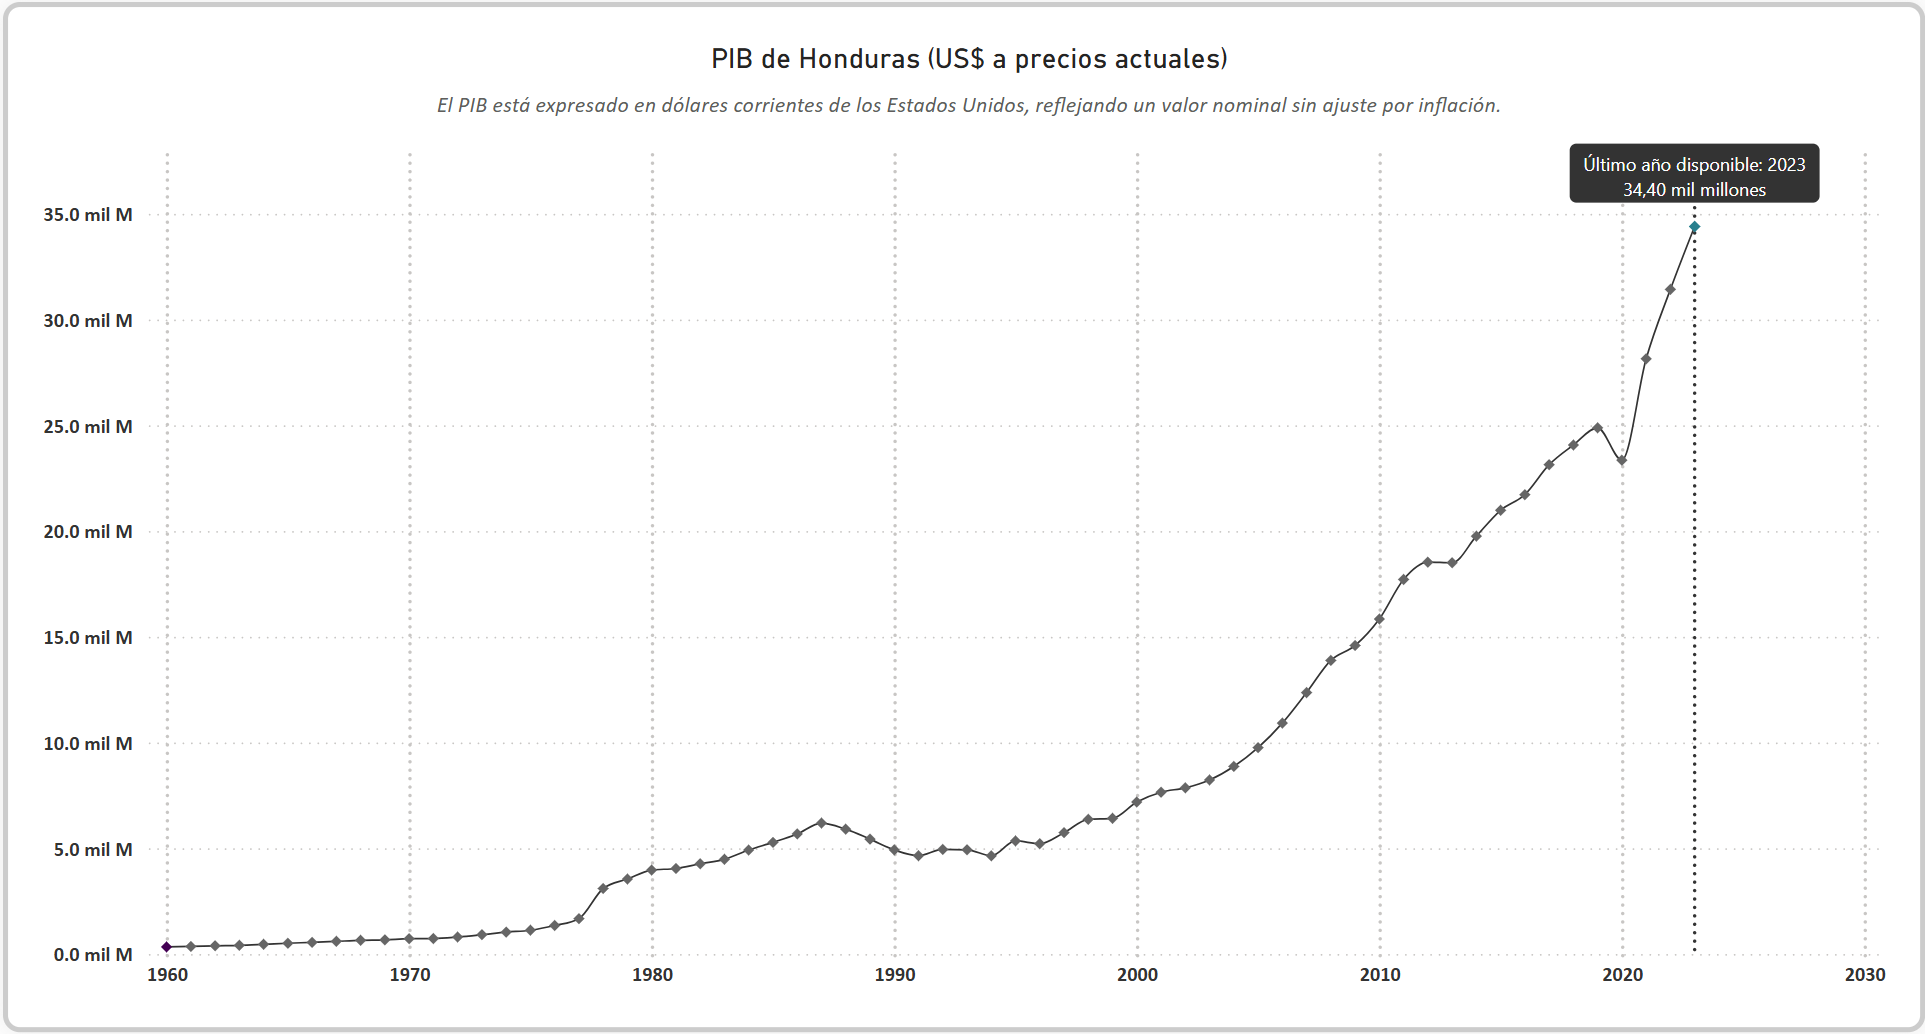
\includegraphics[width=0.85\textwidth]{figures/PIBHNVal.png}
\caption{Evolución del PIB de Honduras en dólares corrientes,
1960--2023.  Fuente:~\cite{WorldBankGDP}.}
\label{fig:PIBHNVal01}
\end{figure}

\subsection{Tasa de crecimiento anual del PIB}

La tasa de crecimiento real del PIB, ajustada por inflación, revela
períodos de expansión y recesión \cite{WorldBankGDPGrowth}.  La
Figura~\ref{fig:PIBHNPer01} expone la volatilidad de este indicador,
con caídas pronunciadas en 2009 y 2020.

\begin{figure}[H]
\centering
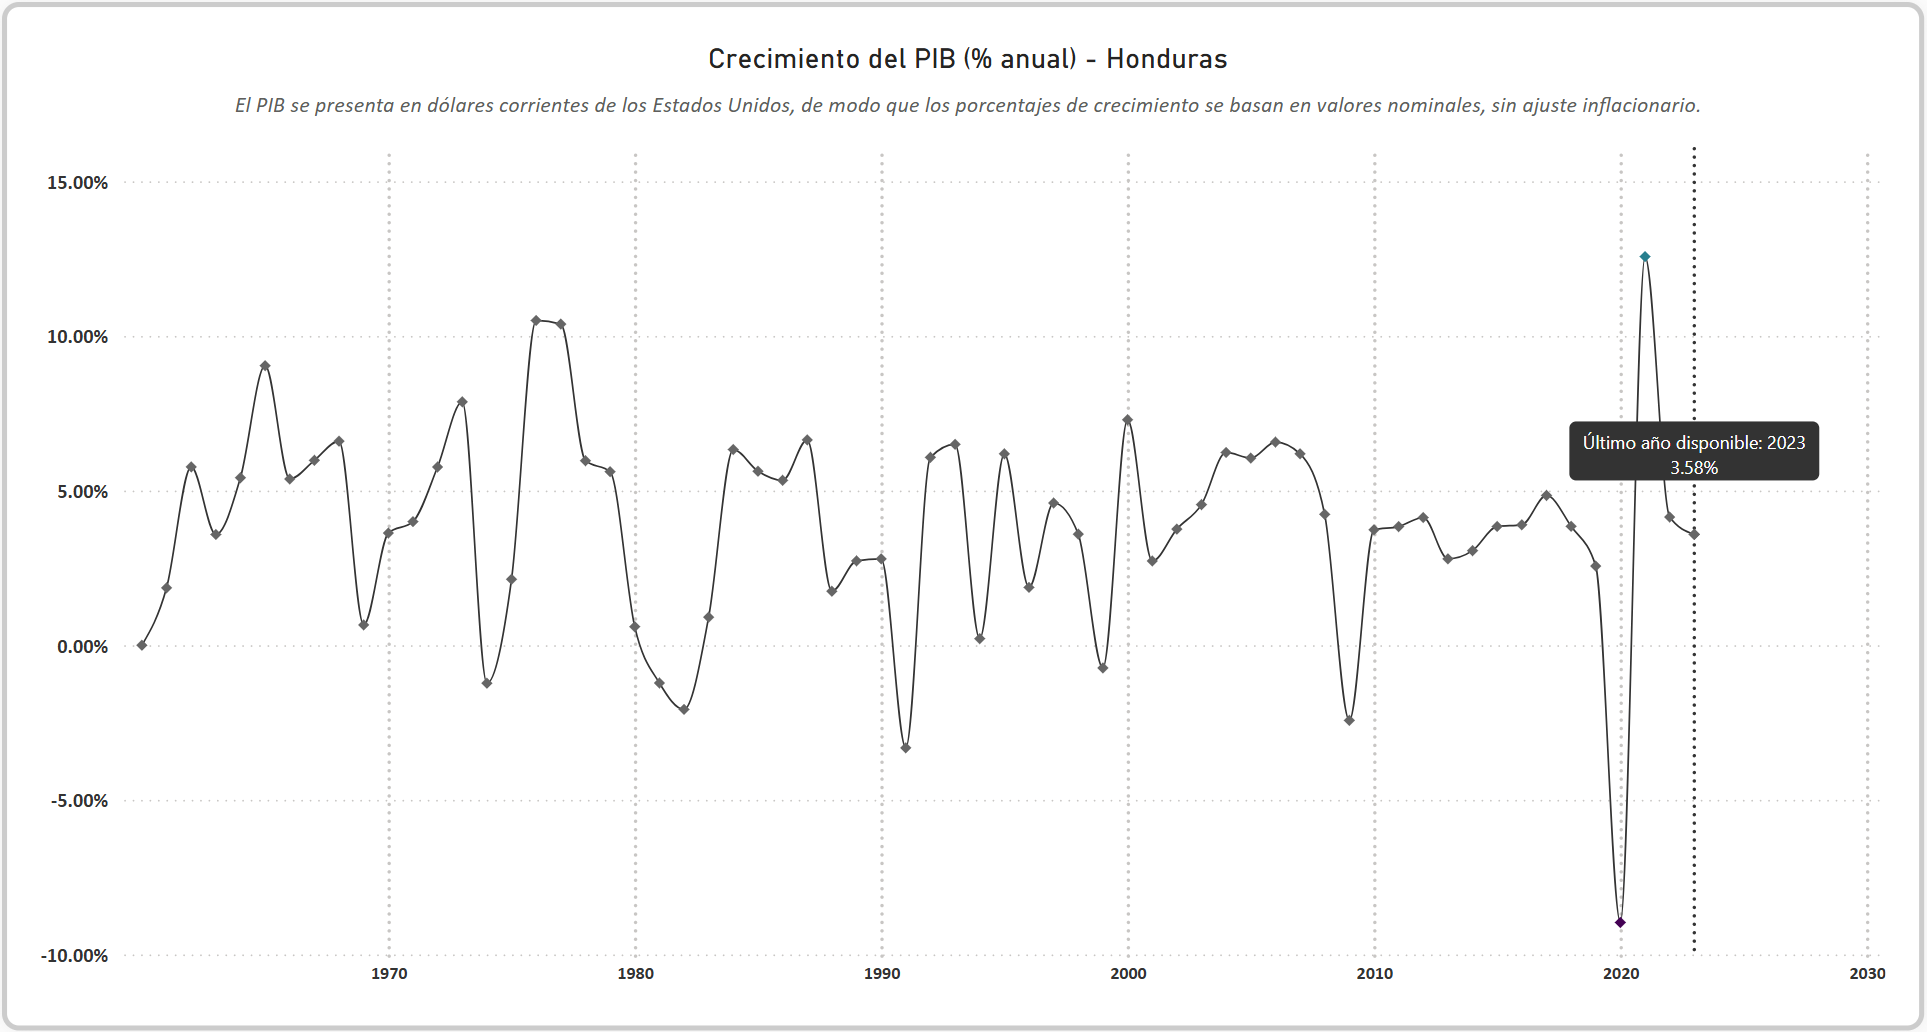
\includegraphics[width=0.85\textwidth]{figures/PIBHNPer.png}
\caption{Tasa de crecimiento anual del PIB de Honduras,
1961--2023.  Fuente:~\cite{WorldBankGDPGrowth}.}
\label{fig:PIBHNPer01}
\end{figure}

\subsection{PIB per cápita en dólares corrientes}

El PIB per cápita ofrece una aproximación a la prosperidad promedio y
al nivel de vida \cite{WorldBankGDPPC}.  Su trayectoria, visible en
la Figura~\ref{fig:PIBHNCap01}, es fundamental para evaluar el
desarrollo económico en términos humanos.

\begin{figure}[H]
\centering
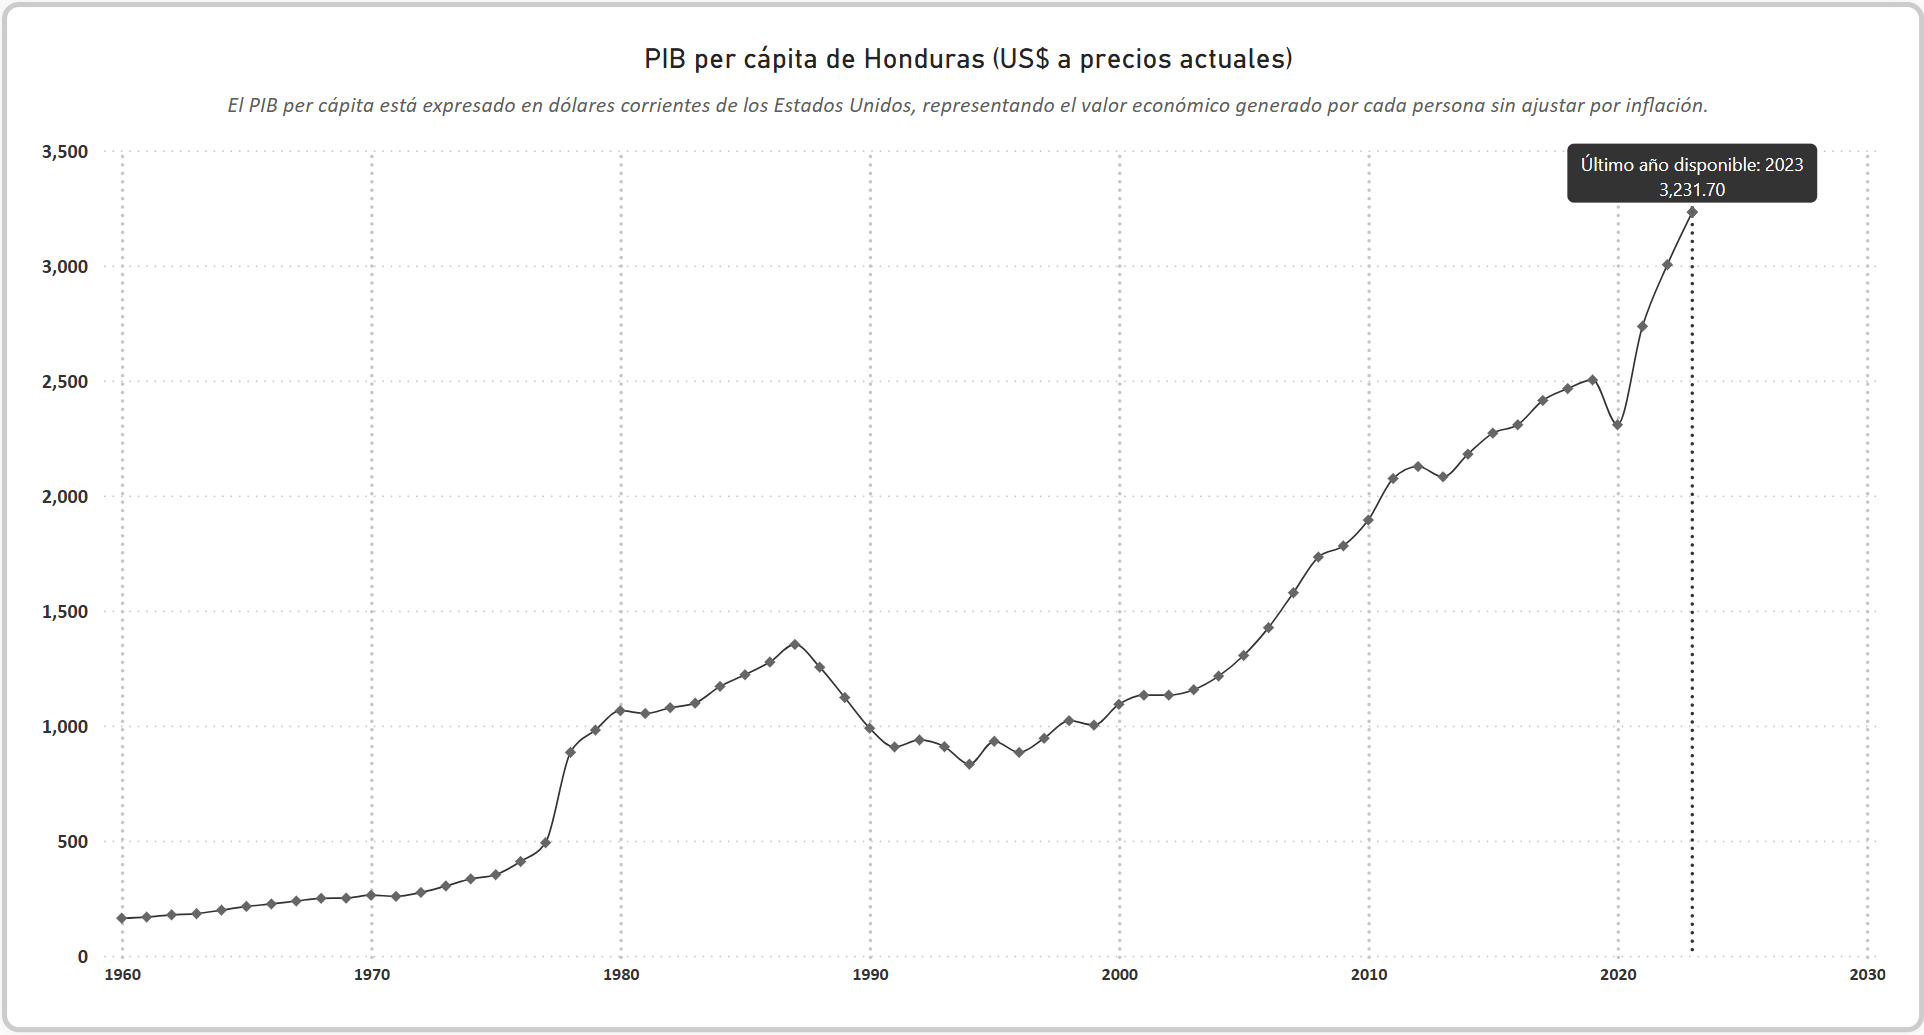
\includegraphics[width=0.9\textwidth]{figures/PIBHNCap.png}
\caption{PIB per cápita de Honduras en dólares corrientes,
1960--2023.  Fuente:~\cite{WorldBankGDPPC}.}
\label{fig:PIBHNCap01}
\end{figure}

\subsection{PIB per cápita en lempiras a precios constantes}

Esta es la serie de referencia principal para los análisis de los
Capítulos~\ref{cap:tcroc} y~\ref{cap:tcroc_hibrido_integrado}.
Al estar denominada en moneda local y a precios constantes, elimina
los efectos tanto de la inflación como de las fluctuaciones del tipo
de cambio, ofreciendo la medida más pura de la producción real por
habitante \cite{WorldBankGDPPCConst}.

\begin{figure}[H]
\centering
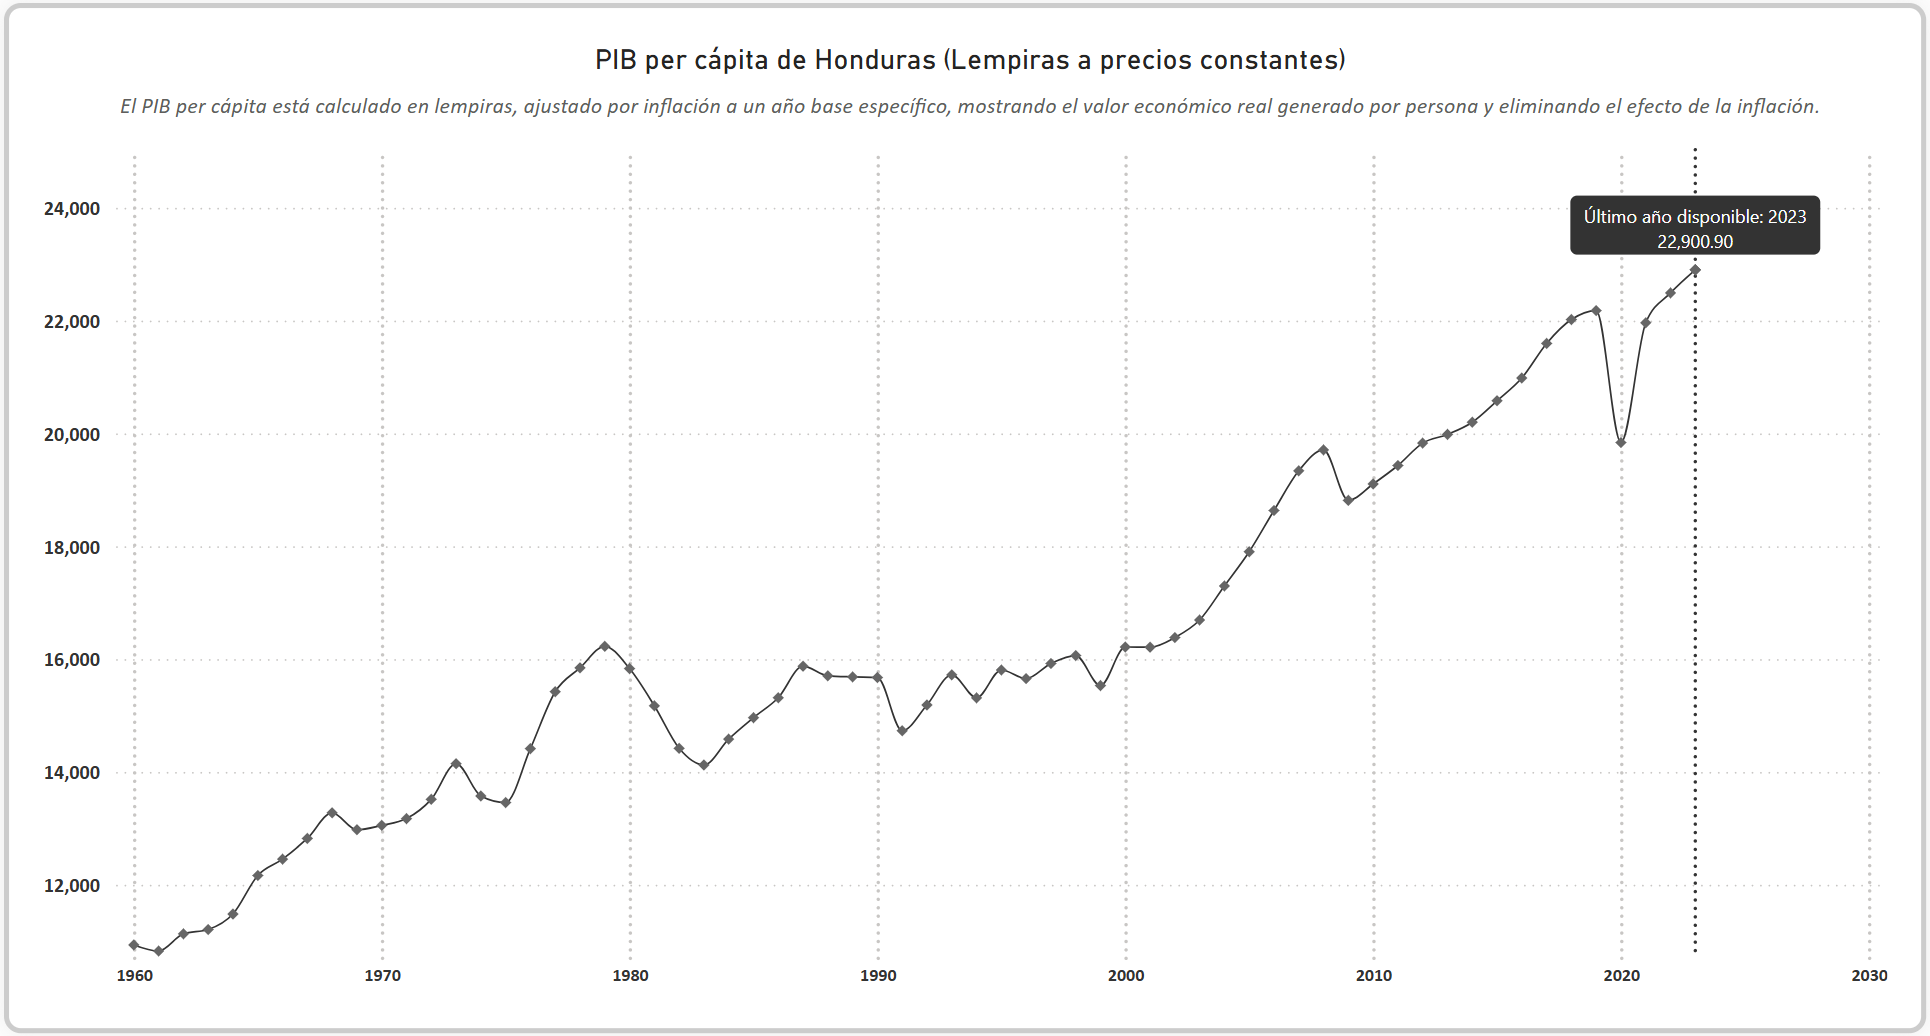
\includegraphics[width=0.9\textwidth]{figures/PIBHNCapConst.png}
\caption{PIB per cápita de Honduras en lempiras a precios
constantes, 1960--2023.  Fuente:~\cite{WorldBankGDPPCConst}.}
\label{fig:PIBHNCapConst01}
\end{figure}

La Tabla~\ref{tbl:SeriesEvolution} resume numéricamente la evolución
de estas series para el período de estudio principal (2000--2023),
que sirve de base para la estimación de los modelos.

\begin{table}[H]
\centering
\caption{Evolución de series económicas seleccionadas de Honduras,
2000--2023.}
\label{tbl:SeriesEvolution}
\resizebox{\textwidth}{!}{%
\begin{tabular}{|c|r|r|r|r|}
\hline
\textbf{Año} & \textbf{PIB Dólares Corr.\ (M\,USD)} &
\textbf{Crec.\ Anual (\%)} &
\textbf{PIB p.c.\ Dólares (USD)} &
\textbf{PIB p.c.\ Lempiras Const.} \\ \hline
2000 & 7\,186\,638\,029 & 7.29 & 1\,092.6 & 16\,214.3 \\
2001 & 7\,651\,162\,302 & 2.72 & 1\,132.2 & 16\,211.7 \\
2002 & 7\,858\,255\,413 & 3.75 & 1\,132.5 & 16\,381.9 \\
2003 & 8\,230\,391\,347 & 4.55 & 1\,156.1 & 16\,692.9 \\
2004 & 8\,869\,299\,234 & 6.23 & 1\,215.1 & 17\,296.5 \\
2005 & 9\,757\,012\,697 & 6.05 & 1\,304.7 & 17\,903.1 \\
2006 & 10\,917\,477\,066 & 6.57 & 1\,425.8 & 18\,634.1 \\
2007 & 12\,361\,257\,681 & 6.19 & 1\,577.7 & 19\,337.8 \\
2008 & 13\,881\,731\,876 & 4.23 & 1\,732.5 & 19\,708.9 \\
2009 & 14\,587\,496\,229 & $-2.43$ & 1\,781.2 & 18\,813.3 \\
2010 & 15\,839\,344\,592 & 3.73 & 1\,893.3 & 19\,104.7 \\
2011 & 17\,710\,275\,685 & 3.84 & 2\,073.7 & 19\,431.7 \\
2012 & 18\,528\,554\,398 & 4.13 & 2\,126.0 & 19\,828.9 \\
2013 & 18\,499\,729\,215 & 2.79 & 2\,081.1 & 19\,983.0 \\
2014 & 19\,756\,533\,972 & 3.06 & 2\,179.9 & 20\,199.1 \\
2015 & 20\,979\,791\,685 & 3.84 & 2\,271.2 & 20\,579.2 \\
2016 & 21\,717\,604\,952 & 3.89 & 2\,307.3 & 20\,982.7 \\
2017 & 23\,136\,247\,991 & 4.84 & 2\,413.0 & 21\,595.6 \\
2018 & 24\,067\,750\,760 & 3.84 & 2\,464.6 & 22\,019.3 \\
2019 & 24\,882\,225\,742 & 2.56 & 2\,502.3 & 22\,177.7 \\
2020 & 23\,352\,232\,484 & $-8.97$ & 2\,307.6 & 19\,838.3 \\
2021 & 28\,144\,331\,507 & 12.57 & 2\,735.1 & 21\,961.6 \\
2022 & 31\,426\,041\,807 & 4.14 & 3\,003.3 & 22\,491.3 \\
2023 & 34\,400\,509\,852 & 3.58 & 3\,231.7 & 22\,900.9 \\
\hline
\end{tabular}%
}
\end{table}

% ===================================================================
\section[Precios de Combustibles]{Precios de Combustibles como Serie
de Alta Frecuencia}
\label{sec:combustibles_serie}
% ===================================================================

Para contrastar la dinámica macroeconómica de baja frecuencia del
PIB, se analiza un conjunto de series de mercado de alta frecuencia:
los precios semanales de los combustibles en Honduras.  Estas series
son particularmente valiosas porque reflejan de manera casi
instantánea las volatilidades de los mercados internacionales y las
políticas de precios locales.  Los datos, que abarcan desde
\textbf{2017 hasta 2025}, fueron construidos para esta investigación
mediante un meticuloso proceso de \textit{web scraping} del portal
Proceso Digital \cite{ProcesoHN2025}, seguido de una rigurosa
limpieza y estructuración.  Estas series constituyen el banco de
pruebas empírico del
Capítulo~\ref{cap:regimenes_combustibles}.

\subsection{Precio de la Gasolina Superior}

La evolución del precio de la gasolina superior es un indicador
sensible tanto a los precios internacionales del crudo como a la
demanda interna.

\begin{figure}[H]
\centering
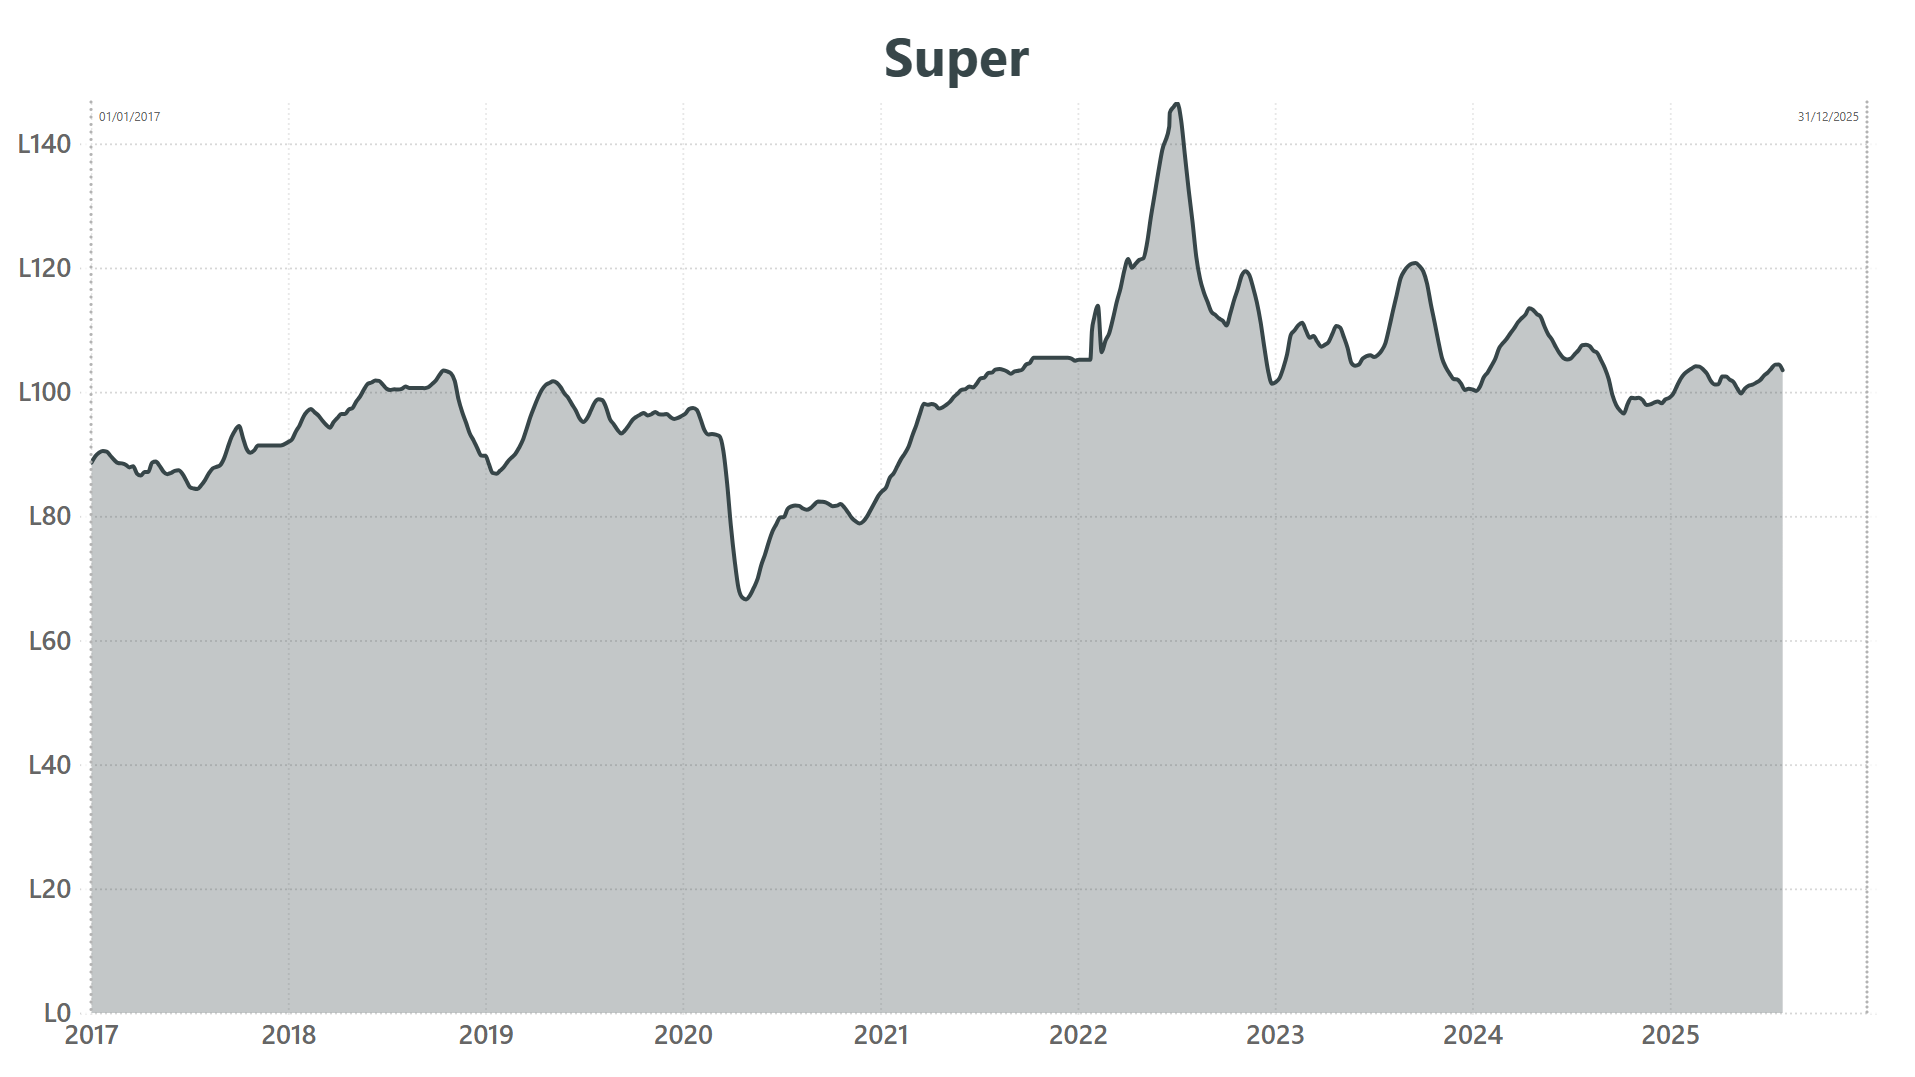
\includegraphics[width=0.95\textwidth]{figures/precio_super.png}
\caption{Precio semanal de la gasolina Superior en Honduras.}
\label{fig:precio_super}
\end{figure}

\subsection{Precio de la Gasolina Regular}

Siendo el combustible de mayor consumo, su precio tiene un impacto
directo en el costo de transporte y, por ende, en la inflación al
consumidor.

\begin{figure}[H]
\centering
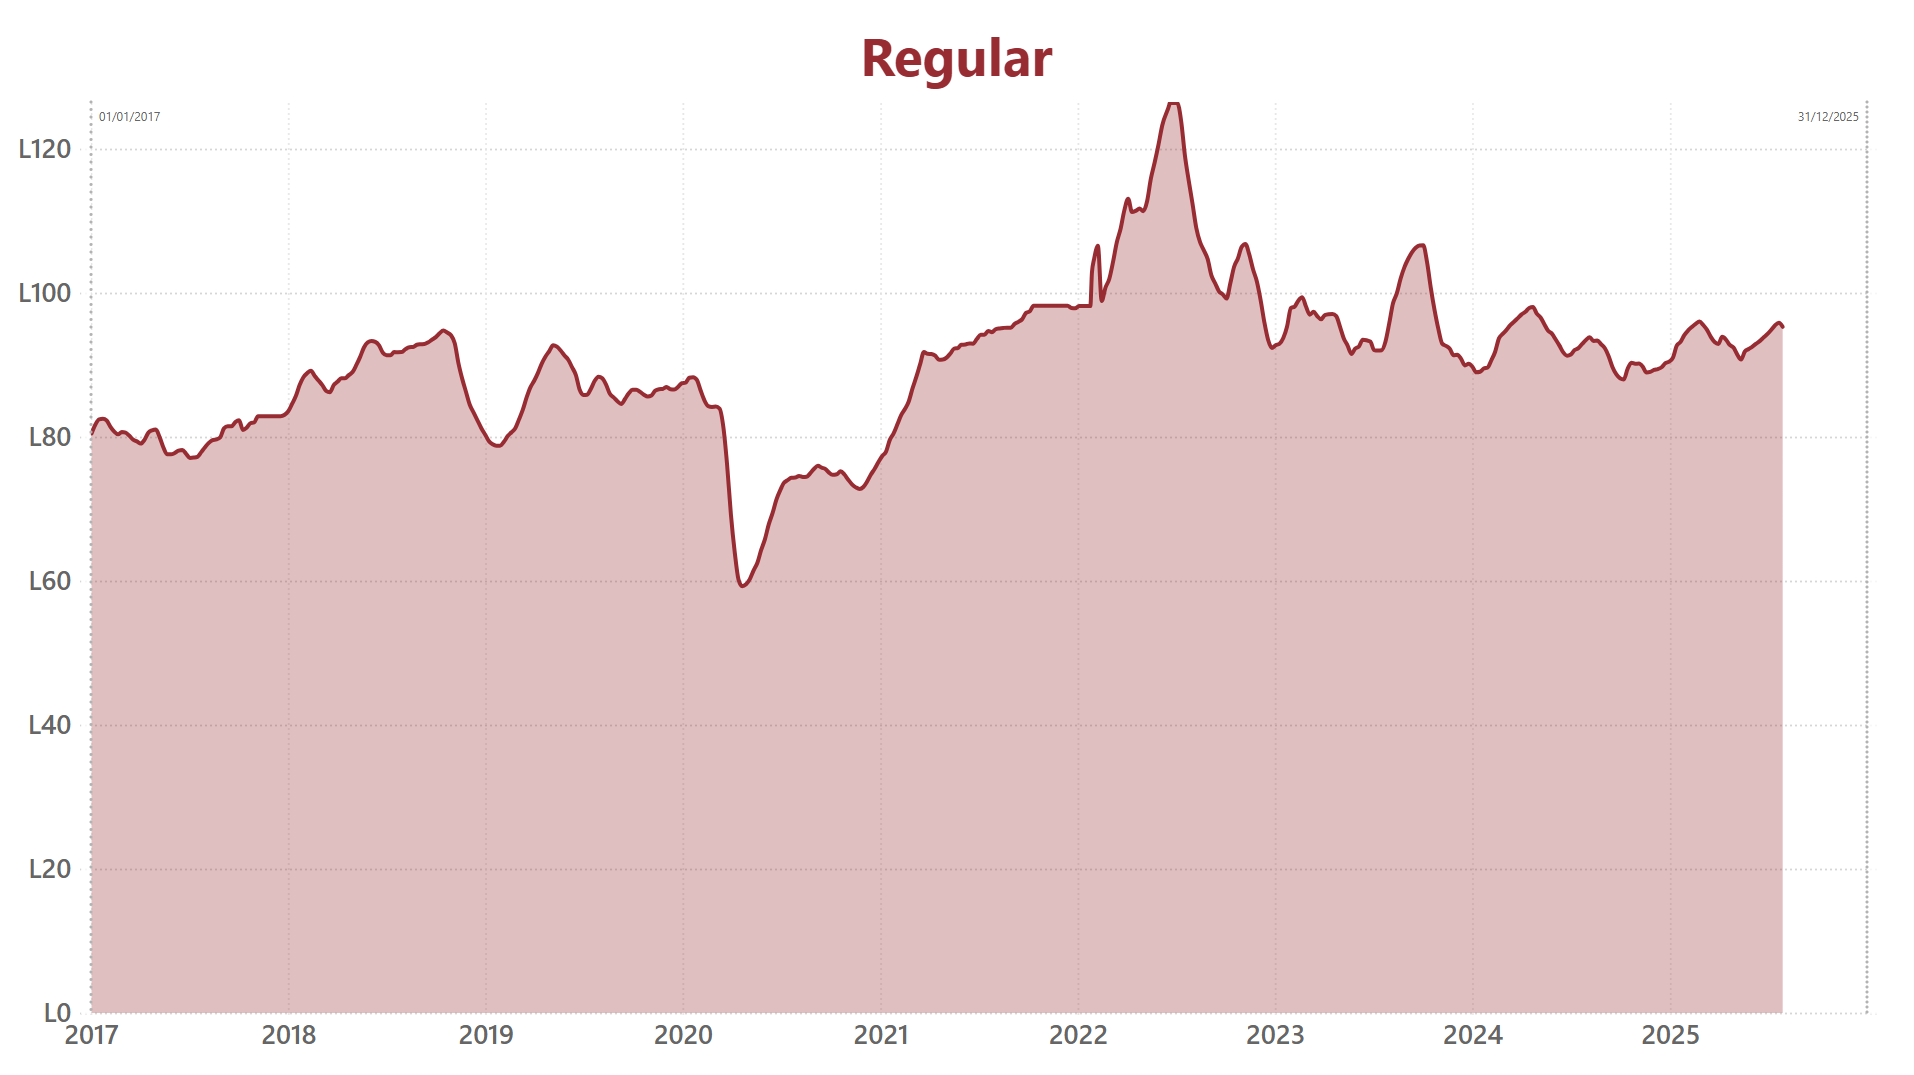
\includegraphics[width=0.95\textwidth]{figures/precio_regular.png}
\caption{Precio semanal de la gasolina Regular en Honduras.}
\label{fig:precio_regular}
\end{figure}

\subsection{Precio del Diésel}

El diésel es fundamental para el transporte de carga y la industria,
por lo que sus fluctuaciones afectan directamente los costos de
producción y la cadena de suministro del país.

\begin{figure}[H]
\centering
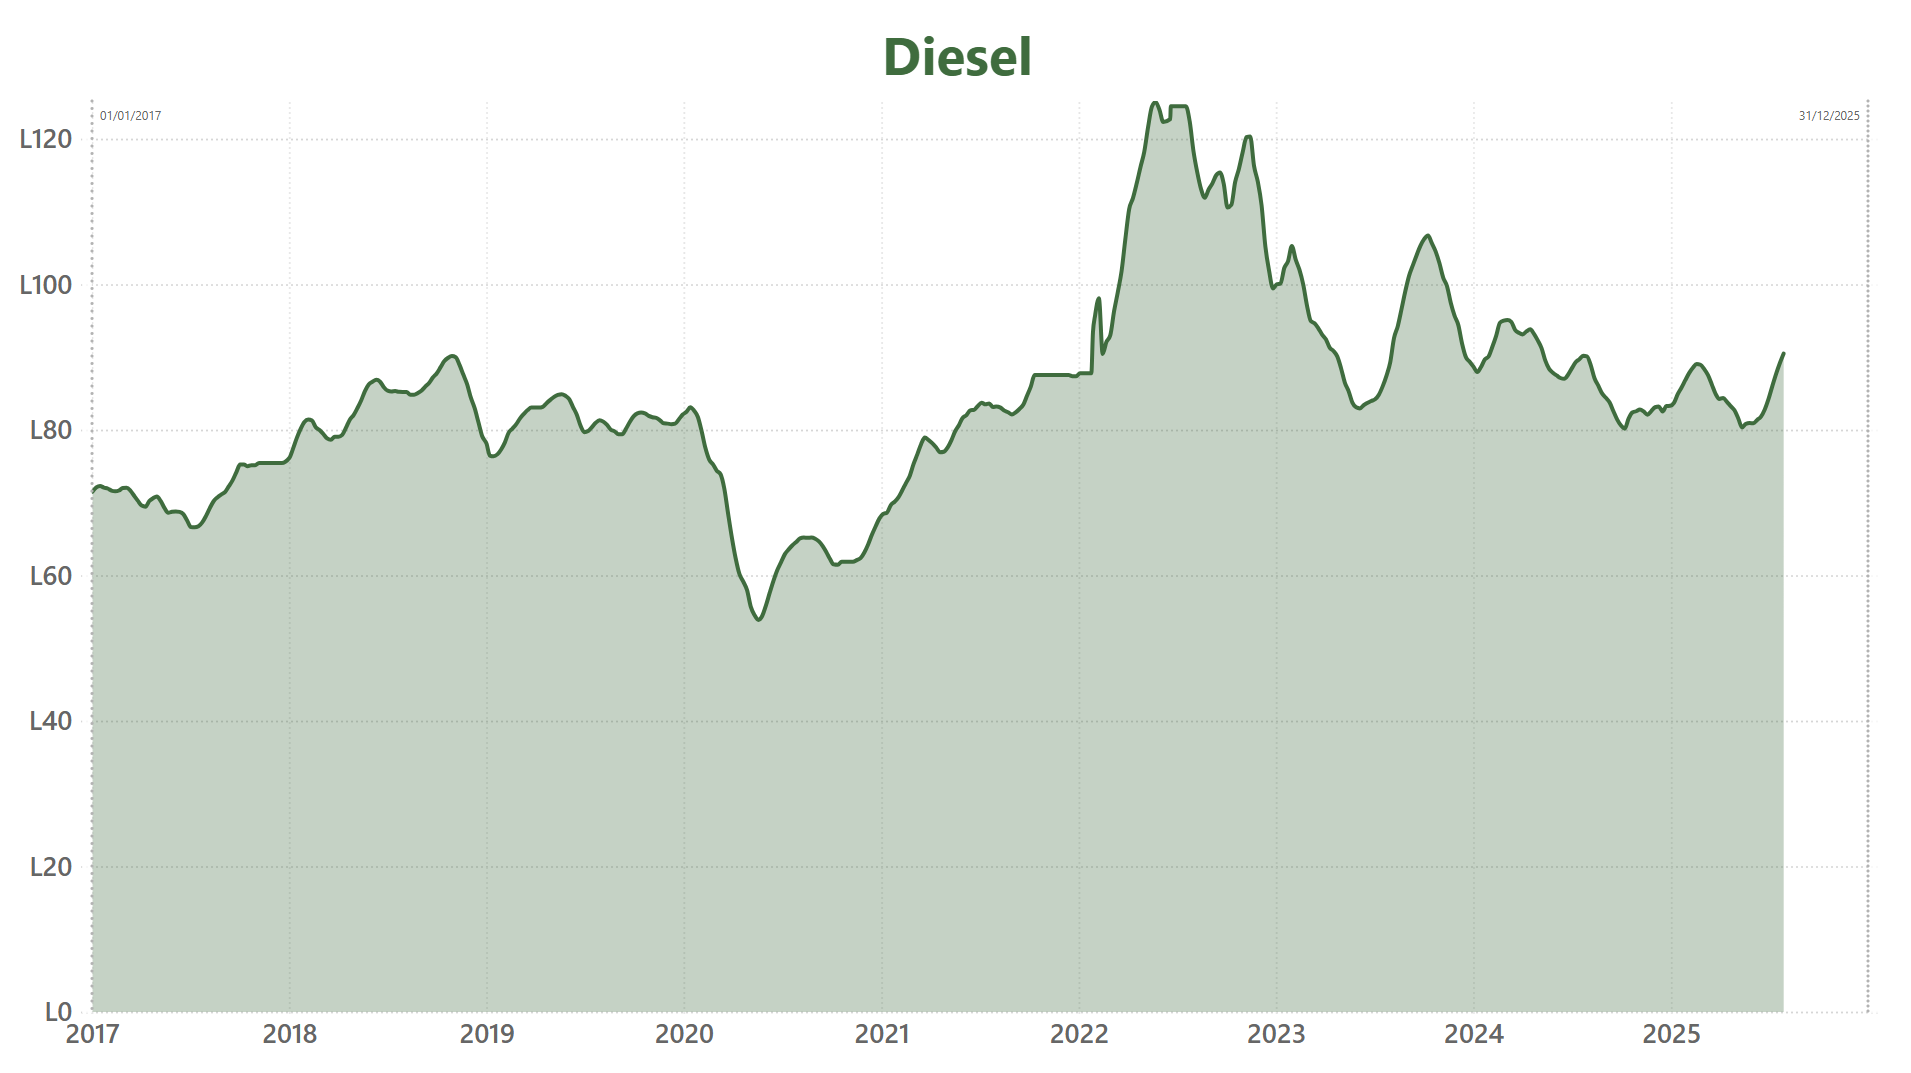
\includegraphics[width=0.95\textwidth]{figures/precio_diesel.png}
\caption{Precio semanal del Diésel en Honduras.}
\label{fig:precio_diesel}
\end{figure}

\subsection{Precio del Kerosene}

Utilizado principalmente para fines domésticos en zonas rurales, el
precio del kerosene es un indicador con importantes implicaciones
sociales.

\begin{figure}[H]
\centering
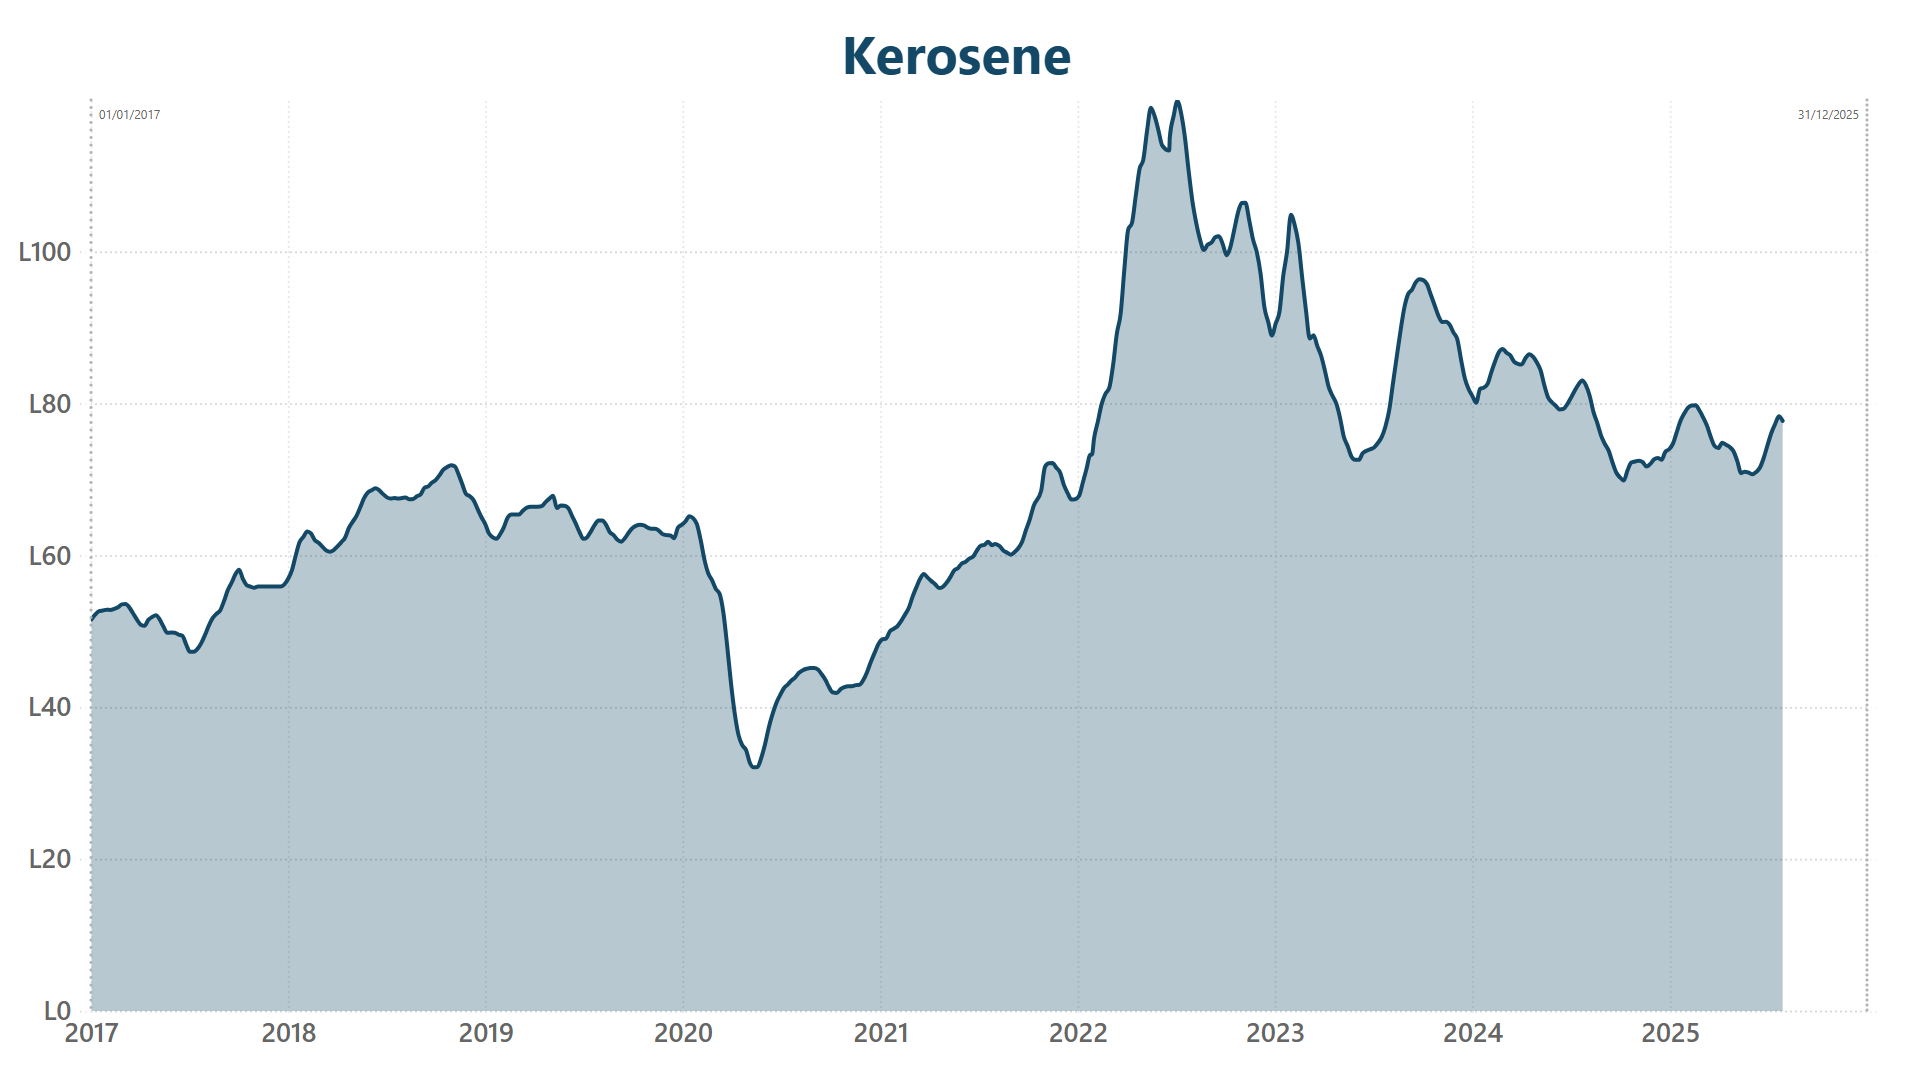
\includegraphics[width=0.95\textwidth]{figures/precio_kerosene.png}
\caption{Precio semanal del Kerosene en Honduras.}
\label{fig:precio_kerosene}
\end{figure}

En conclusión, la elección de estas dos familias de series ---el PIB
como indicador macroeconómico estructural y los combustibles como
indicadores de mercado volátiles--- proporciona un campo de pruebas
diverso y robusto.  Esta dualidad permite validar la eficacia del
modelo TCROC y sus extensiones estocásticas para capturar dinámicas
económicas fundamentalmente distintas, demostrando su versatilidad y
aplicabilidad general.

\include{CAPITULOS/CAP03_Planteamiento}
\chapter{Tasa de Cambio Relativa Óptima Conmutada y sus Variantes}
\label{cap:tcroc}

% -------------------------------------------------------------------
% Introducción

% --- SECCIÓN: Introducción y Motivación Matemática ---
\section{Introducción y Motivación Matemática}
\label{sec:tcroc_introduccion}

El análisis riguroso de fenómenos económicos modelados mediante Cadenas de Markov Ocultas (HMM) o procesos estocásticos de salto de régimen (Markov-Switching) requiere que el espacio de estados subyacente refleje transiciones dinámicas estacionarias o localmente estables. No obstante, las series temporales en finanzas y economía suelen ser altamente no estacionarias y dominadas por ruido. 

En este capítulo se cimenta la base matemática requerida para preparar y transformar la serie temporal cruda antes de someterla a cualquier proceso riguroso de \textbf{discretización de estados}. Se desarrolla formalmente la familia de transformaciones denominada \textbf{Tasa de Cambio Relativa Óptima Conmutada (TCROC)} y sus tres variantes operacionales: la \textbf{TCROCM} (con ventana móvil), la \textbf{ETCROC} (con decaimiento exponencial) y su forma general \textbf{ETCROCM} (con decaimiento exponencial y ventana móvil).

El objetivo de este capítulo es demostrar que el operador TCROC transforma una serie en tiempo discreto $\{v(t)\}_{t=0}^T$ en una secuencia continua de tasas de cambio $\{\alpha_t\}$ mediante la minimización convexa de $v(t) \approx (1+\alpha_t)v(t-1)$. Se demuestra que esta transformación satisface existencia, unicidad, continuidad y estabilidad frente a perturbaciones, propiedades necesarias para que la posterior discretización mediante K-Means produzca agrupaciones consistentes y evite asignaciones de régimen espurias.

Todas las variantes admiten solución analítica cerrada y tienen menor complejidad computacional que métodos iterativos como la máxima verosimilitud en MS-AR. Este capítulo constituye el primer bloque teórico de la tesis: se presentan los teoremas, lemas y demostraciones de consistencia que fundamentan el operador.

% Axiomática del Operador

% --- SECCIÓN: Axiomática del Operador de Tasa de Cambio Local ---
\section{Axiomática del Operador de Tasa de Cambio Local}
\label{sec:tcroc_axiomas}

Para que la transformación $\mathcal{T}: \mathbb{R}^{T+1} \to \mathbb{R}^T$ que genera la secuencia $\{\alpha_t\}$ sea compatible con una posterior discretización en cadena de Markov, debe satisfacer un conjunto mínimo de propiedades algebraicas y analíticas. La familia TCROC se construye de modo que cumpla los siguientes cuatro axiomas:

\begin{description}
    \item[Axioma 1 (Localidad Acotada y Dependencia Estricta):]
    El estado continuo de la tasa de cambio en un instante $t$,
    denotado como $\alpha_t$, depende exclusivamente de un
    subconjunto cerrado del pasado inmediato $[t-W+1, t]$.  Esta
    dependencia captura la dinámica inercial de los mercados y
    rechaza la influencia de estados temporales infinitamente
    lejanos.
    \item[Axioma 2 (Proporcionalidad Geométrica Local):] La relación entre valores consecutivos se modela como $v(t) = \beta_t\, v(t-1) + \varepsilon_t$. La tasa de cambio $\alpha_t = \beta_t - 1$ representa la variación relativa local entre observaciones adyacentes.
    \item[Axioma 3 (Unicidad y Convexidad Global):] El escalar $\alpha_t$ se obtiene como el mínimo global de una funcional de costo estrictamente convexa en $L^2$, lo que garantiza unicidad de la solución.
    \item[Axioma 4 (Estabilidad de Lipschitz frente a Perturbaciones):]
    Existe una constante $C > 0$ tal que variaciones acotadas en la
    serie observada $\|v' - v\|_\infty \leq \epsilon$ inducen
    desviaciones finitamente controladas en la proyección:
    \[
    |\alpha' - \alpha| \leq C\epsilon,
    \]
    lo que garantiza que la discretización posterior sea robusta ante ruido en los datos.
\end{description}

A lo largo de este capítulo se demostrará matemáticamente que las diferentes instanciaciones del modelo base (TCROC, TCROCM, ETCROC y ETCROCM) satisfacen integralmente estos axiomas.

% --- SECCIÓN: Marco General Unificado ---
\section{Marco General Unificado}
\label{sec:tcroc_marco_general}

Sea \(T > 0\) un entero y \(\Sigma_T = \{v(0), v(1), \dots, v(T)\}\) una serie temporal con \(v(t) \in \mathbb{R}\). Dados un tamaño de ventana \(W\) con \(1 \leq W \leq T\) y un factor de decaimiento \(\lambda \in (0, 1]\), definimos para cada instante \(t \geq W\) la \textbf{tasa de cambio relativa óptima generalizada} como:

\begin{equation}
    \alpha_{t,\lambda,W} \;:=\; -1 + \arg\min_{\beta \in \mathbb{R}} \sum_{k=t-W+1}^{t} \lambda^{t-k} \bigl(v(k) - \beta\, v(k-1)\bigr)^2.
\label{eq:tcroc_general}
\end{equation}

Las cuatro variantes se recuperan como casos particulares:

\begin{center}
\renewcommand{\arraystretch}{1.3}
\begin{tabular}{lcc}
\toprule
\textbf{Variante} & \textbf{Parámetros} & \textbf{Notación} \\
\midrule
TCROC   & \(\lambda = 1,\; W = T\) & \(\alpha_T\) \\
TCROCM  & \(\lambda = 1,\; W < T\) & \(\alpha_{t}^{(W)}\) \\
ETCROC  & \(\lambda < 1,\; W = T\) & \(\alpha_{T,\lambda}\) \\
ETCROCM & \(\lambda < 1,\; W < T\) & \(\alpha_{t,\lambda,W}\) \\
\bottomrule
\end{tabular}
\end{center}

Esta estructura jerárquica se ilustra en la Figura~\ref{fig:jerarquia_tcroc}.

\begin{figure}[htbp]
    \centering
    \begin{tikzpicture}[
        node distance=1.5cm and 2.8cm,
        >=Stealth,
        % --- Estilos (mismos que Cap 5) ---
        base/.style={draw, rectangle, rounded corners=6pt, minimum width=3.2cm, 
                     minimum height=0.9cm, font=\small\bfseries, align=center,
                     drop shadow={shadow xshift=1pt, shadow yshift=-1pt, opacity=0.3}},
        canonical/.style={base, fill=nordSnow, draw=nordGray, text=nordDark},
        extension/.style={base, fill=nordSnow, draw=nordGray, text=nordDark},
        hybrid/.style={base, fill=nordSnow!80!nordFrost, draw=nordFrost, text=nordDark},
        edgelabel/.style={font=\scriptsize, fill=white, inner sep=2pt, opacity=0.9}
    ]

        % Nodos
        \node[canonical] (TCROC) {TCROC\\{\scriptsize $(W=T,\;\lambda=1)$}};
        
        \node[extension] (TCROCM) [below left=of TCROC] {TCROCM\\{\scriptsize $(W<T)$}};
        \node[extension] (ETCROC) [below right=of TCROC] {ETCROC\\{\scriptsize $(\lambda<1)$}};
        
        \node[hybrid] (ETCROCM) [below=2.8cm of TCROC] {ETCROCM\\{\scriptsize $(W<T,\;\lambda<1)$}};

        % Conexiones
        \draw[->, thick] (TCROC) -- (TCROCM) node[edgelabel, midway, left] {$+\,W$};
        \draw[->, thick] (TCROC) -- (ETCROC) node[edgelabel, midway, right] {$+\,\lambda$};
        \draw[->, thick] (TCROCM) -- (ETCROCM) node[edgelabel, midway, left] {$+\,\lambda$};
        \draw[->, thick] (ETCROC) -- (ETCROCM) node[edgelabel, midway, right] {$+\,W$};

        % Conexión directa (punteada)
        \draw[->, thick, dashed, nordGray!60] (TCROC) -- (ETCROCM)
            node[edgelabel, midway] {$(W, \lambda)$};

    \end{tikzpicture}
    \caption{Jerarquía paramétrica del operador TCROC y sus variantes. El nodo central representa la formulación global canónica ($W=T, \lambda=1$). La incorporación de memoria restringida ($W<T$) y decaimiento exponencial ($\lambda < 1$) producen las extensiones laterales, que convergen en el operador generalizado ETCROCM.}
    \label{fig:jerarquia_tcroc}
\end{figure}

% Propiedades Analíticas del Operador Generalizado

% --- SECCIÓN: Teoremas Fundamentales del Operador Generalizado ---
\section{Teoremas Fundamentales del Operador Generalizado}
\label{sec:tcroc_teoremas_generales}

Dado que la variante híbrida dinámica (ETCROCM) subsume paramétricamente a las formulaciones base (TCROC, TCROCM y ETCROC), se procede a demostrar las propiedades algebraicas, topológicas y asintóticas directamente sobre la forma generalizada \(\alpha_{t,\lambda,W}\) definida en la Ecuación \eqref{eq:tcroc_general}. Las demostraciones y garantías matemáticas para el resto de las variantes se infieren de manera colateral e inmediata por simple relajación o límite de parámetros.

Esta consolidación eleva el rigor analítico, demostrando que cualquier filtro derivado de esta familia cumple forzosamente con el comportamiento axiomático exigido previamente.

% --- SUBSECCIÓN: Existencia Ponderada y Unicidad Global --- - - - - - - - - - - - - - - - - - - - - - - - - - - - - - -
\subsection{Existencia Ponderada y Unicidad Global}
\label{subsec:teorema_existencia}

\begin{theorem}
\label{teo:existencia_general}
Para cualquier instante de tiempo válido \(t \geq W\), si el subconjunto de observaciones contenidas en la ventana local de rezagos exhibe al menos un suceso medible no nulo (formalmente, \(\exists k \in [t-W+1, t]\) tal que \(v(k-1) \neq 0\)), entonces la funcional de costo en el espacio topológico \(L^2\), definida como \(f(\beta) = \sum_{k=t-W+1}^{t} \lambda^{t-k} \bigl(v(k) - \beta\, v(k-1)\bigr)^2\), admite un y solo un minimizador global \(\hat{\beta}_{t,\lambda,W}\) formulado cerradamente por:
\begin{equation}
\hat{\beta}_{t,\lambda,W} = \frac{\displaystyle\sum_{k=t-W+1}^{t} \lambda^{t-k}\, v(k)\, v(k-1)}{\displaystyle\sum_{k=t-W+1}^{t} \lambda^{t-k}\, v(k-1)^2}.
\label{eq:beta_general}
\end{equation}
\end{theorem}

\begin{proof}
Sea $a = \sum_{k=t-W+1}^{t} \lambda^{t-k}\, v(k-1)^2$.  Dado que
$\lambda \in (0,1]$, cada peso $\lambda^{t-k}$ es estrictamente
positivo.  Por la hipótesis de no degeneración, existe al menos un
$k$ tal que $v(k-1) \neq 0$, de donde $a > 0$.  Entonces
$f(\beta) = a\beta^2 - 2b\beta + c$ con $a > 0$ es estrictamente
convexa y coerciva ($f(\beta) \to +\infty$ cuando
$|\beta| \to \infty$).  El mínimo global se alcanza en el único
punto donde $f'(\beta) = 2a\beta - 2b = 0$, es decir,
$\hat{\beta}_{t,\lambda,W} = b/a$, que coincide con la expresión
\eqref{eq:beta_general}.
\end{proof}

\begin{corollary}
\label{cor:etcrocm_alpha}
Bajo las mismas condiciones del Teorema~\ref{teo:existencia_general},
la tasa de cambio relativa
\begin{equation}
\alpha_{t,\lambda,W} = \hat{\beta}_{t,\lambda,W} - 1
\label{eq:alpha_general}
\end{equation}
está bien definida y es única para cada $t \geq W$.
\end{corollary}

Este resultado garantiza que los algoritmos de discretización
posteriores (e.g., K-Means) reciben una entrada bien definida,
evitando divisiones por cero o indeterminaciones numéricas.

% --- SUBSECCIÓN: Consistencia Asintótica Ergódica --- - - - - - - - - - - - - - - - - - - - - - - - - - - - - - -
\subsection{Consistencia Asintótica}
\label{subsec:teorema_consistencia}

\begin{theorem}[Consistencia del estimador]
\label{teo:consistencia_general}
Supóngase que la serie temporal $\{v(k)\}$ satisface localmente
el modelo autorregresivo de primer orden
$v(k) = \beta^* v(k-1) + \varepsilon_k$,
donde $\{\varepsilon_k\}$ es ruido blanco con
$\mathbb{E}[\varepsilon_k] = 0$ y
$\mathbb{E}[\varepsilon_k^2] = \sigma^2 < \infty$,
y $|\beta^*| < 1$ (estacionariedad).  Entonces, cuando
$W \to \infty$ con $\lambda \in (0,1]$ fijo,
\[
\hat{\beta}_{t,\lambda,W} \xrightarrow{p} \beta^*
\quad \text{y, en consecuencia,} \quad
\alpha_{t,\lambda,W} \xrightarrow{p} \beta^* - 1.
\]
\end{theorem}

\begin{proof}
Sustituyendo $v(k) = \beta^* v(k-1) + \varepsilon_k$ en la
expresión del estimador \eqref{eq:beta_general}, se obtiene
\[
\hat{\beta}_{t,\lambda,W}
= \frac{\sum_{k=t-W+1}^{t} \lambda^{t-k}
       (\beta^* v(k-1) + \varepsilon_k)\, v(k-1)}
      {\sum_{k=t-W+1}^{t} \lambda^{t-k}\, v(k-1)^2}
= \beta^* + \frac{N_W}{D_W},
\]
donde
$N_W = \sum_{k} \lambda^{t-k}\, \varepsilon_k\, v(k-1)$ y
$D_W = \sum_{k} \lambda^{t-k}\, v(k-1)^2$.

\textbf{Paso~1 (Denominador).}  Dado que $|\beta^*| < 1$, el proceso
$\{v(k)\}$ es estacionario y ergódico, con
$\mathbb{E}[v(k-1)^2] = \sigma^2/(1 - \beta^{*2}) > 0$.  Sea
$\Lambda_W = \sum_{k=t-W+1}^{t} \lambda^{t-k}$.  Por la Ley de los
Grandes Números para sucesiones ponderadas estacionarias
\cite{Anderson1971},
\[
\frac{D_W}{\Lambda_W} \xrightarrow{p}
\mathbb{E}[v(k-1)^2] = \frac{\sigma^2}{1 - \beta^{*2}} > 0.
\]

\textbf{Paso~2 (Numerador).}  Como $\varepsilon_k$ es independiente
de $\mathcal{F}_{k-1} = \sigma(v(0), \ldots, v(k-1))$, se tiene
$\mathbb{E}[\varepsilon_k v(k-1)] = 0$.  Por la desigualdad de Chebyshev,
\[
\text{Var}\!\left(\frac{N_W}{\Lambda_W}\right)
= \frac{\sum_{k} \lambda^{2(t-k)}\,
       \mathbb{E}[\varepsilon_k^2 v(k-1)^2]}{\Lambda_W^2}
\leq \frac{\sigma^2 \mathbb{E}[v(k-1)^2]
       \sum_{k} \lambda^{2(t-k)}}{\Lambda_W^2}
= \mathcal{O}\!\left(\frac{1}{W}\right) \to 0.
\]

\textbf{Paso~3 (Conclusión).}  Por el Lema de Slutsky,
$N_W / D_W = (N_W/\Lambda_W) / (D_W/\Lambda_W)
\xrightarrow{p} 0 / \mathbb{E}[v(k-1)^2] = 0$.
Por tanto, $\hat{\beta}_{t,\lambda,W} \xrightarrow{p} \beta^*$.
\end{proof}

\begin{remark}[Alcance de la hipótesis de estacionariedad]
\label{rem:estacionariedad}
La hipótesis $|\beta^*| < 1$ es esencial para la prueba, pues
garantiza que $\mathbb{E}[v(k-1)^2]$ sea finito.  Sin embargo, las
series económicas reales (como el PIB nominal) frecuentemente
exhiben tendencia, con $\beta^*$ cercano o igual a 1.  En tales
casos, el Teorema~\ref{teo:consistencia_general} no es directamente
aplicable a la serie $v(t)$ en niveles.

No obstante, el operador $\alpha_{t,\lambda,W}$ actúa como un
filtro de diferenciación local: $\alpha_t \approx v(t)/v(t-1) - 1$,
que es análogo a la tasa de crecimiento.  Para una serie con raíz
unitaria ($\beta^* = 1$), la serie de tasas
$\alpha_t = v(t)/v(t-1) - 1$ es generalmente estacionaria.  En la
implementación empírica, la consistencia se verifica por la
estacionariedad de $\{\alpha_t\}$, no necesariamente de $\{v(t)\}$.
La validación con tests ADF aplicados a la serie
$\{\alpha_t\}$ se presenta en el
Capítulo~\ref{cap:regimenes_combustibles}.
\end{remark}

% --- SUBSECCIÓN: Estabilidad de Lipschitz --- - - - - - - - - - - -
\subsection{Estabilidad de Lipschitz}
\label{subsec:teorema_estabilidad}

El Axioma~4 requiere que el operador sea robusto frente a
perturbaciones acotadas en los datos de entrada.  El siguiente lema
formaliza esta propiedad.

\begin{lemma}[Estabilidad tipo Lipschitz]
\label{lem:estabilidad_general}
Sean $\{v(k)\}$ y $\{v'(k)\}$ dos series tales que
$\|v' - v\|_\infty \leq \epsilon$ (perturbación uniforme acotada).
Defínase
$S_2 = \sum_{k=t-W+1}^{t} \lambda^{t-k}\, v(k-1)^2 > 0$.
Entonces
\[
|\alpha'_{t,\lambda,W} - \alpha_{t,\lambda,W}|
\leq C_t \cdot \epsilon,
\]
donde $C_t$ es una constante que depende de $v$, $\lambda$ y $W$,
satisfaciendo
$C_t = \mathcal{O}\!\bigl(\|v\|_{\ell^2} / S_2\bigr)$.
\end{lemma}

\begin{proof}
Sean $S_1 = \sum_k \omega_k\, v(k)v(k-1)$ y
$S_1' = \sum_k \omega_k\, v'(k)v'(k-1)$, con
$\omega_k = \lambda^{t-k}$.  Escribiendo $v'(k) = v(k) + \delta(k)$
con $|\delta(k)| \leq \epsilon$:
\begin{align*}
S_1' - S_1 &= \sum_k \omega_k\bigl[
  v(k)\delta(k-1) + \delta(k)v(k-1) + \delta(k)\delta(k-1)
\bigr].
\end{align*}
Por la desigualdad de Cauchy-Schwarz y la cota
$|\delta(k)| \leq \epsilon$:
\[
|S_1' - S_1| \leq 2\epsilon \sum_k \omega_k |v(k)| \cdot |v(k-1)|
+ \epsilon^2 \sum_k \omega_k
\leq 2\epsilon \Lambda_W \|v\|_{\ell^2}^2 / W + \epsilon^2 \Lambda_W.
\]
De manera análoga, $|S_2' - S_2| \leq
2\epsilon\sum_k \omega_k |v(k-1)| + \epsilon^2 \Lambda_W$.
Como $\alpha = S_1/S_2 - 1$, la diferencia
$|\alpha' - \alpha| = |S_1'/S_2' - S_1/S_2|$ se acota
mediante la fórmula del cociente:
\[
\left|\frac{S_1'}{S_2'} - \frac{S_1}{S_2}\right|
= \frac{|S_1' S_2 - S_1 S_2'|}{S_2 S_2'}
\leq \frac{S_2|S_1'-S_1| + |S_1||S_2'-S_2|}{S_2 S_2'}.
\]
Dado que $S_2' \geq S_2 - \mathcal{O}(\epsilon) > 0$ para
$\epsilon$ suficientemente pequeño, todos los términos del
numerador son lineales en $\epsilon$ (los cuadráticos en $\epsilon$
son de orden inferior), obteniéndose $|\alpha' - \alpha|
\leq C_t \epsilon$ con
$C_t = \mathcal{O}(\|v\|_{\ell^2} / S_2)$.
\end{proof}

% --- SUBSECCIÓN: Optimalidad de Gauss-Markov --- - - - - - - - - -
\subsection{Optimalidad de Gauss-Markov}
\label{subsec:teorema_optimalidad}

\begin{theorem}[Optimalidad GLS del estimador]
\label{teo:optimalidad_general}
Considérese el modelo lineal local
$v(k) = \beta\, v(k-1) + \varepsilon_k$ con errores
heterocedásticos cuya varianza decrece con la antigüedad:
$\mathrm{Var}(\varepsilon_k) = \sigma^2 / \lambda^{t-k}$,
donde $\lambda \in (0,1]$.  Entonces el estimador
$\hat{\beta}_{t,\lambda,W}$ definido en \eqref{eq:beta_general}
coincide con el \textbf{Estimador de Mínimos Cuadrados
Generalizados (GLS)} del modelo, y por el Teorema de
Gauss-Markov generalizado, es el estimador lineal insesgado de
mínima varianza (BLUE).
\end{theorem}

\begin{proof}
Bajo el modelo $\vect{v} = \beta\,\vect{v}_{-1} + \vect{\varepsilon}$
con $\mathrm{Cov}(\vect{\varepsilon}) = \sigma^2 \mat{\Omega}$,
donde $\mat{\Omega} = \mathrm{diag}(\lambda^{-(t-k)})_{k=t-W+1}^{t}$,
el estimador GLS es
\[
\hat{\beta}_{\text{GLS}}
= (\vect{v}_{-1}^T \mat{\Omega}^{-1} \vect{v}_{-1})^{-1}
  \vect{v}_{-1}^T \mat{\Omega}^{-1} \vect{v}.
\]
Como $\mat{\Omega}^{-1} = \mathrm{diag}(\lambda^{t-k})$, se tiene
\[
\hat{\beta}_{\text{GLS}}
= \frac{\sum_{k} \lambda^{t-k}\, v(k)\, v(k-1)}
      {\sum_{k} \lambda^{t-k}\, v(k-1)^2}
= \hat{\beta}_{t,\lambda,W},
\]
que coincide exactamente con el estimador ETCROCM.  La propiedad
BLUE se sigue del Teorema de Gauss-Markov generalizado
\cite{Aitken1936, Anderson1971}.
\end{proof}

% --- SECCIÓN: Casos Particulares del Estimador Generalizado ---
\section{Casos Particulares del Estimador Generalizado}
\label{sec:tcroc_corolarios}

Las variantes de la familia TCROC presentadas en la
Sección~\ref{sec:tcroc_introduccion} surgen como casos particulares
del estimador generalizado $\hat{\beta}_{t,\lambda,W}$ al
especializar los parámetros $W$ y $\lambda$.  A continuación se
formaliza cada variante como un corolario del
Teorema~\ref{teo:existencia_general}.

% --- SUBSECCIÓN: TCROC ---
\subsection{TCROC: Estimador Global
(\texorpdfstring{$W=T,\;\lambda=1$}{W=T, lambda=1})}

Al fijar $W = T$ y $\lambda = 1$, todos los pesos son unitarios
y la sumatoria abarca la totalidad de la serie.  El estimador se
reduce a
\begin{equation}
\hat{\beta}_T = \frac{\sum_{k=1}^{T} v(k)\, v(k-1)}
                    {\sum_{k=1}^{T} v(k-1)^2},
\qquad \alpha_T = \hat{\beta}_T - 1.
\label{eq:tcroc_global}
\end{equation}
Este estimador produce un escalar constante $\alpha_T$ que resume
la tendencia global de la serie.  Al no depender de $t$, sirve
como línea base (\textit{baseline}) contra la cual se comparan las
variantes locales.

\begin{remark}[Degeneración del TCROC global]
\label{rem:degeneracion_tcroc}
Dado que $\alpha_T$ es un escalar único para toda la serie, la
secuencia de estados discretos $S_t = \pi(\alpha_T)$ es constante:
todos los instantes se asignan al mismo régimen.  En consecuencia,
el modelo TCROC-Markov se vuelve trivial (la matriz de transición es
la identidad).  Esta degeneración se confirma empíricamente
en el Capítulo~\ref{cap:regimenes_combustibles}.  Por este
motivo, la variante TCROC ($W = T$, $\lambda = 1$) tiene un
rol exclusivamente teórico dentro de la jerarquía: sirve como
caso límite y línea base, pero en la práctica se emplean las
variantes locales (TCROCM, ETCROC, ETCROCM) con $W \ll T$.
\end{remark}

% --- SUBSECCIÓN: TCROCM ---
\subsection{TCROCM: Estimador con Ventana Móvil
(\texorpdfstring{$W<T,\;\lambda=1$}{W<T, lambda=1})}

Al restringir la ventana a $W < T$ pero manteniendo $\lambda = 1$
(pesos uniformes), el estimador utiliza únicamente las $W$
observaciones más recientes:
\begin{equation}
\hat{\beta}_{t}^{(W)} = \frac{\sum_{k=t-W+1}^{t} v(k)\, v(k-1)}
                            {\sum_{k=t-W+1}^{t} v(k-1)^2},
\qquad \alpha_t^{(W)} = \hat{\beta}_{t}^{(W)} - 1.
\label{eq:tcrocm}
\end{equation}
Esto produce una secuencia $\{\alpha_t^{(W)}\}_{t=W}^{T}$ que se
actualiza en cada instante, de manera análoga a una media móvil
autoregresiva.  La longitud $W$ controla el compromiso entre
sensibilidad local y estabilidad del estimador.

% --- SUBSECCIÓN: ETCROC ---
\subsection{ETCROC: Estimador con Decaimiento Exponencial
(\texorpdfstring{$W=T,\;\lambda<1$}{W=T, lambda<1})}

Al utilizar toda la muestra ($W = T$) pero con factor de
decaimiento $\lambda \in (0,1)$, las observaciones recientes
reciben mayor peso que las antiguas de forma geométrica:
\begin{equation}
\hat{\beta}_{T,\lambda} = \frac{\sum_{k=1}^{T} \lambda^{T-k}\,
  v(k)\, v(k-1)}{\sum_{k=1}^{T} \lambda^{T-k}\, v(k-1)^2},
\qquad \alpha_{T,\lambda} = \hat{\beta}_{T,\lambda} - 1.
\label{eq:etcroc}
\end{equation}
El factor $\lambda$ actúa como un filtro exponencial que suaviza
la señal $\alpha_t$ con respecto a la TCROCM, reduciendo la
sensibilidad a variaciones puntuales.  Esto la convierte en la
variante preferida como paso previo a la discretización por
K-Means en el marco TCROC-Markov
(Capítulos~\ref{cap:TCROC-Markov}--\ref{cap:tcroc_hibrido_integrado}).

% Complejidad Algorítmica Comparativa

% --- SECCIÓN: Complejidad Algorítmica ---
\section{Complejidad Algorítmica}
\label{sec:tcroc_complejidad}

El cálculo de cada variante depende de dos sumatorias:
\[
S_1 = \sum \omega_k\, v(k)\, v(k-1), \qquad S_2 = \sum \omega_k\, v(k-1)^2,
\]
donde \(\omega_k\) es el peso correspondiente y el rango de la suma depende de la variante.

\begin{table}[H]
\centering
\caption{Comparativa de complejidad algorítmica.}
\label{tab:tcroc_complejidad}
\begin{tabular}{@{}lll@{}}
\toprule
\textbf{Método} & \textbf{Complejidad} & \textbf{Operaciones dominantes} \\
\midrule
TCROC   & \(\mathcal{O}(T)\)            & Sumatorias globales \\
ETCROC  & \(\mathcal{O}(T)\)            & Sumatorias recursivas con decaimiento \\
TCROCM  & \(\mathcal{O}(T \cdot W)\)    & Sumatorias por ventana móvil \\
ETCROCM & \(\mathcal{O}(T \cdot W)\)    & Sumatorias ponderadas por ventana \\
\midrule
OLS     & \(\mathcal{O}(T)\)            & Operaciones básicas \\
MLE     & \(\mathcal{O}(T^2)\text{--}\mathcal{O}(T^3)\) & Optimización iterativa \\
ARIMA   & \(\mathcal{O}(T^2)\)          & Optimización iterativa \\
Redes neuronales & \(\mathcal{O}(T \cdot L)\) & Backpropagation (\(L\): capas) \\
\bottomrule
\end{tabular}
\end{table}

La ETCROC admite una implementación recursiva eficiente mediante
\[
S_1(t) = \lambda\, S_1(t-1) + v(t)\, v(t-1), \qquad S_2(t) = \lambda\, S_2(t-1) + v(t-1)^2,
\]
que reduce el cálculo incremental a \(\mathcal{O}(1)\) por observación.

\begin{figure}[H]
\centering
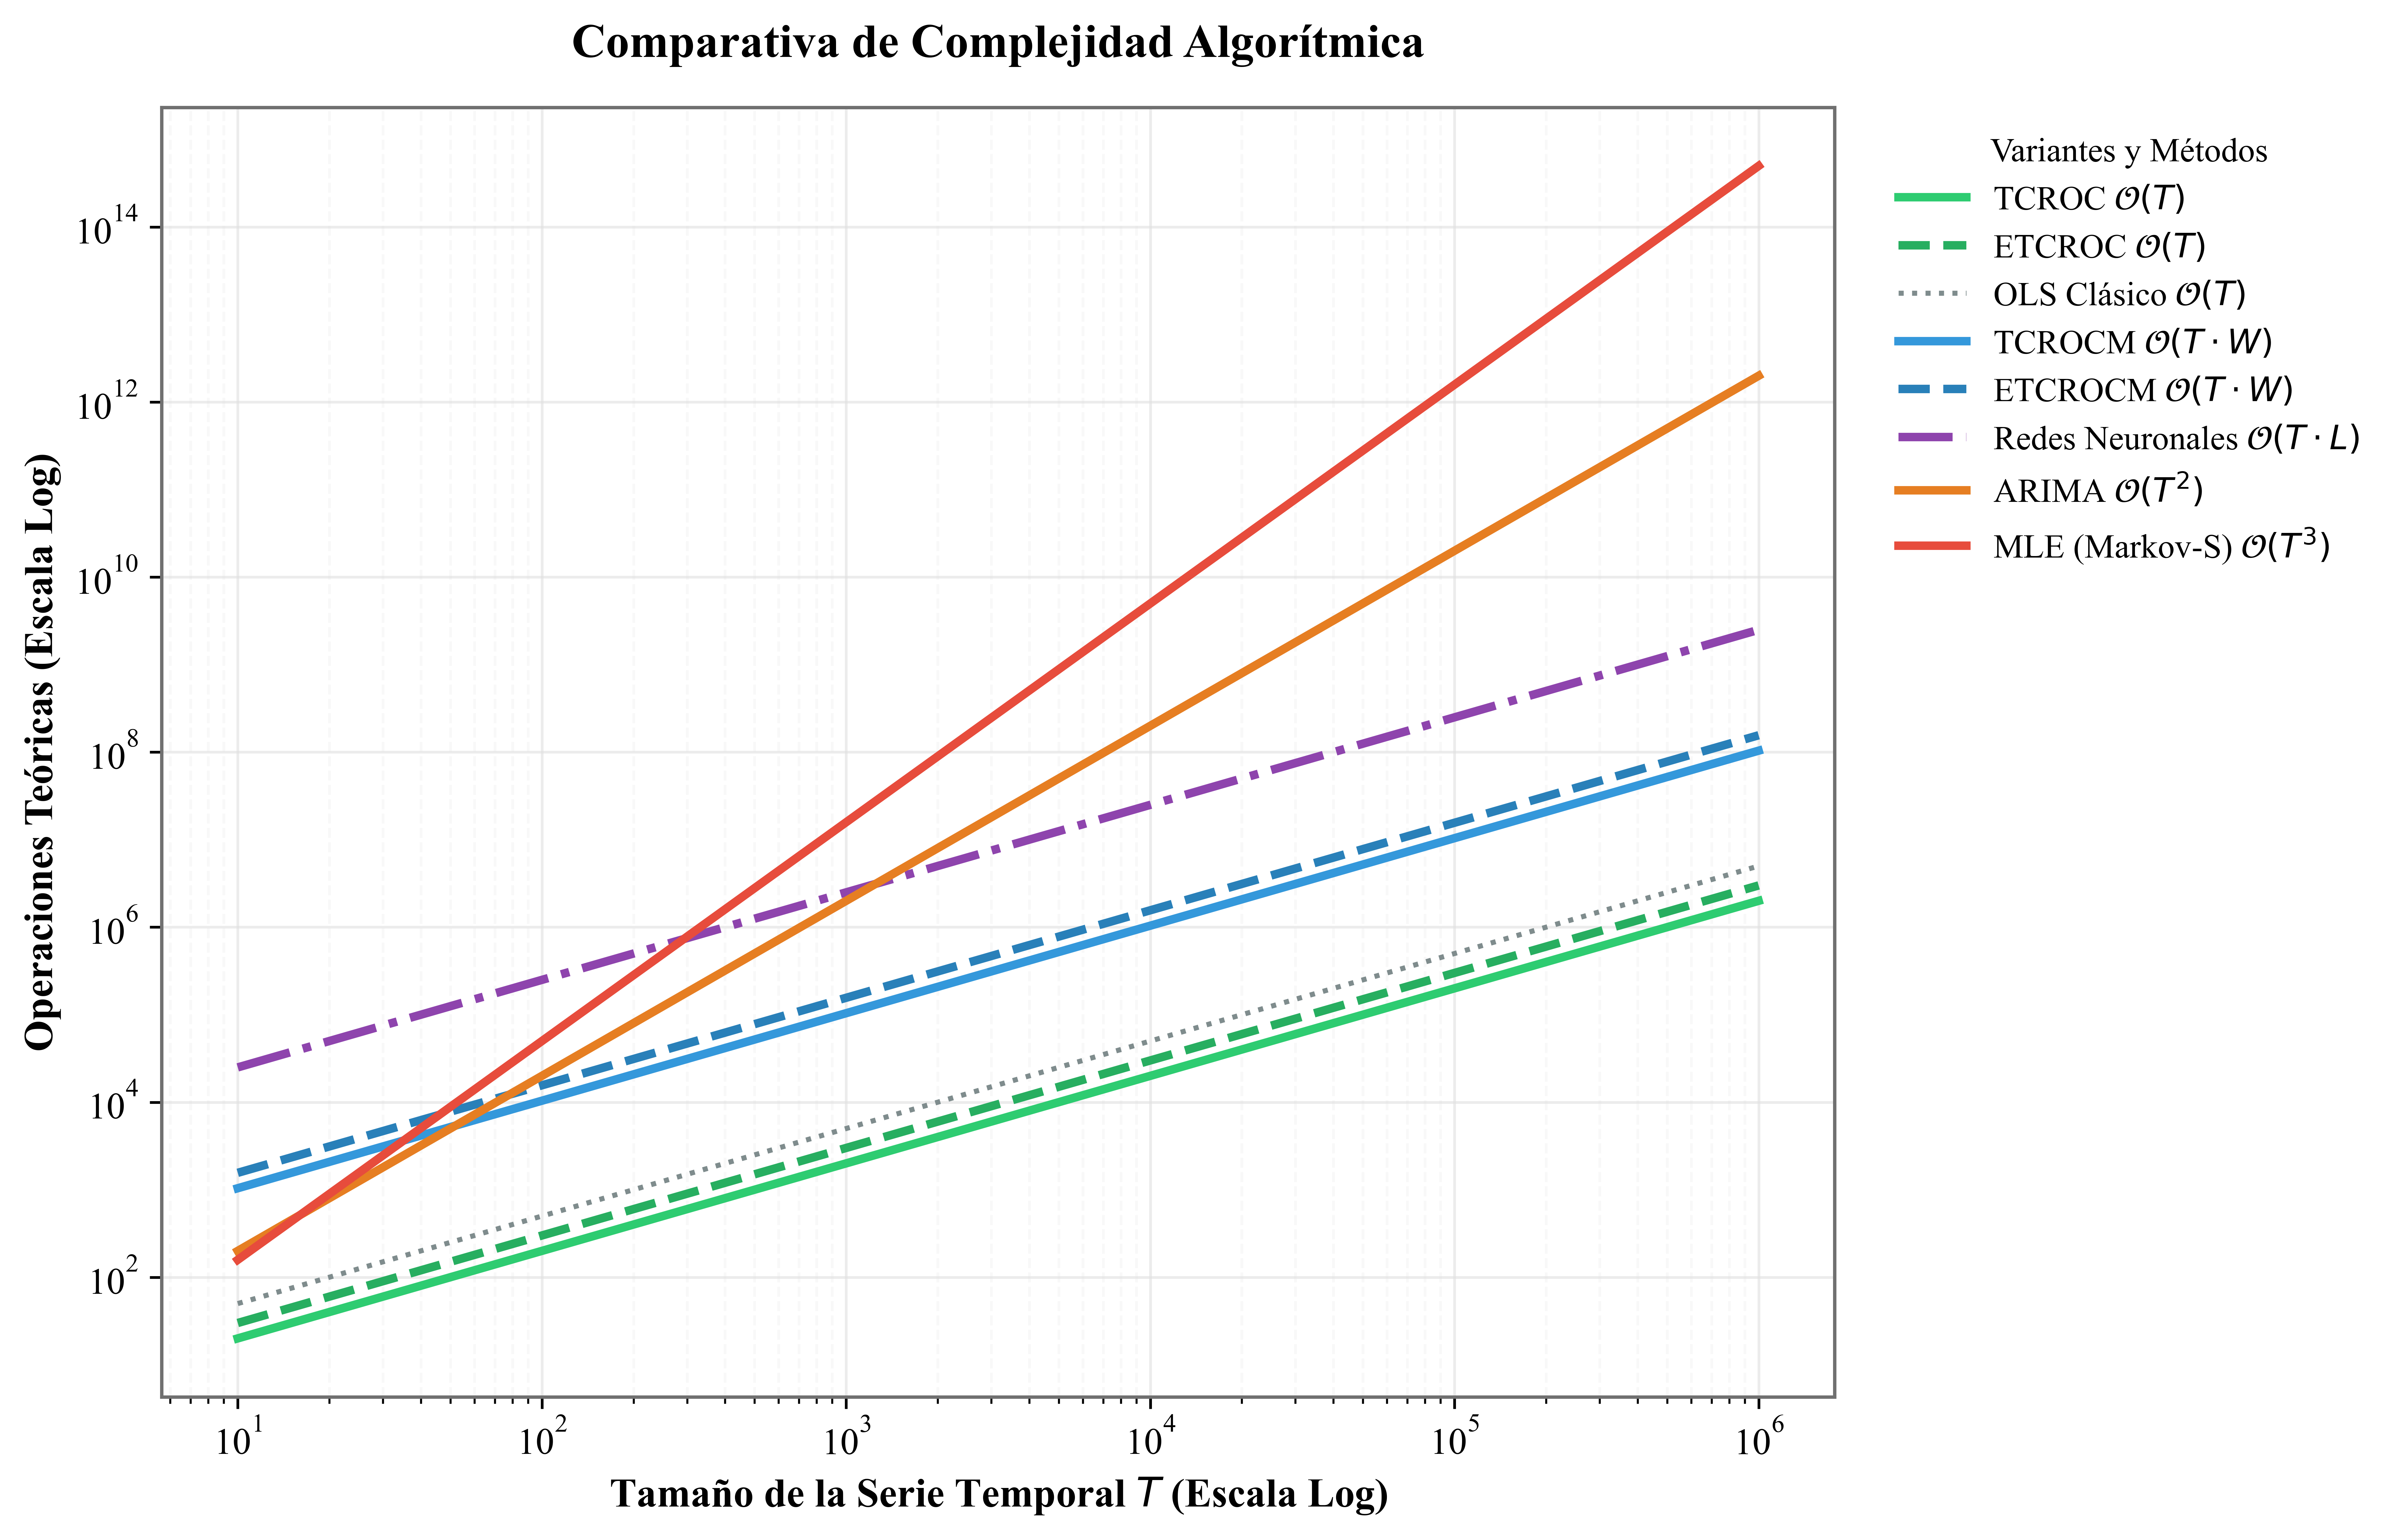
\includegraphics[width=\textwidth]{figures/CompTodosMeto.png}
\caption{Comparativa de complejidad: TCROC, TCROCM, ETCROC, ETCROCM, OLS, MLE, Redes Neuronales y ARIMA.}
\label{fig:tcroc_comp_todos}
\end{figure}

% Implementación Computacional

% --- SECCIÓN: Implementación Computacional ---
\section{Implementación Computacional}
\label{sec:tcroc_implementacion}

La siguiente función unificada en Python calcula cualquier variante de la TCROC según los parámetros proporcionados:

\begin{listing}[H]
\begin{python}
import numpy as np

def compute_tcroc(v, W=None, lambd=1.0):
    """
    Operador unificado matemáticamente eficiente para la familia TCROC.
    Calcula el escalar beta y el mapeo proyectivo alpha bajo el marco L^2.

    Parámetros
    ----------
    v : array_like (Longitud T+1)
        Vector secuencia de observaciones temporales.
    W : int, opcional
        Tamaño de la ventana (truncamiento de memoria). Si es None, W = T.
    lambd : float, opcional
        Factor amnésico de decaimiento en (0, 1]. Default: 1.0.

    Retorna
    -------
    alpha (float): Tasa de cambio relativa proyectada.
    beta (float): Factor inercial multiplicativo óptimo.
    """
    v = np.asarray(v, dtype=float)
    T = len(v) - 1
    
    # Axioma 1: Restricción Local
    if W is None or W > T:
        W = T
    elif W < 1:
        raise ValueError("La ventana local W debe ser >= 1.")

    start = T - W + 1
    v_target = v[start : T+1]
    v_lag    = v[start-1 : T]

    # Vectorización absoluta del decaimiento L^2 (evita bucles for lentos)
    # Secuencia de pesos: [lambda^(W-1), lambda^(W-2), ..., 1]
    weights = lambd ** np.arange(W - 1, -1, -1) if lambd != 1.0 else 1.0

    # Axioma 3: Solución de Mínimos Cuadrados Ponderados (Dot products en C)
    num = np.sum(weights * v_target * v_lag)
    den = np.sum(weights * (v_lag ** 2))

    if den == 0:
        raise ValueError("Degeneración algebraica: Varianza rezagada nula.")

    beta = num / den
    alpha = beta - 1.0
    
    return alpha, beta
\end{python}
\caption{Función unificada en Python para calcular las variantes de la TCROC.}
\label{lst:tcroc_implementacion}
\end{listing}

% Ejemplos Numéricos

% --- SECCIÓN: Ejemplos Numéricos Sectoriales (Perspectiva a 2026) ---
\section[Ejemplos Numéricos Sectoriales]{Ejemplos Numéricos Sectoriales (Perspectiva a 2026)}
\label{sec:tcroc_ejemplos}

Para validar empíricamente la asimilación matemática del operador, se aplica la familia TCROC sobre la macro-dimensión del \textbf{PIB en Dólares Corrientes} de la República de Honduras (periodo 2000--2024, con \(T = 24\) intervalos o transiciones observadas). Se estiman las proyecciones resultantes bajo los cuatro esquemas de asimilación paramétrica estudiados para los años fiscales 2025 y 2026.

\begin{examplex}[Proyecciones del PIB Corriente - Variante Base y Extensiones]
\label{ex:pib_dolares_2026}
Sea la secuencia empírica del PIB en dólares corrientes (millones USD) cerrando el año fiscal 2024 con un valor histórico auditado de \(37,093.57\) millones USD. 

Bajo la \textbf{TCROC global (\(W=T, \lambda=1\))}, el sumatorio agnóstico completo hereda una inercia constante \(\hat{\beta} \approx 1.0704\), indicando una tasa de asimilación proyectiva estricta de \(\alpha_T \approx 7.04\%\). 

No obstante, las perturbaciones dinámicas recientes se capturan de forma asimétrica permitiendo el ajuste de memoria y el decaimiento. En la Tabla~\ref{tab:proy_tcroc_pib}, se modelizan los escenarios inerciales divergentes según el ensamble paramétrico de pre-condicionamiento que será entregado a los agrupadores de Markov.

\begin{table}[H]
\centering
\begin{tabular}{@{}lccc@{}}
\toprule
\textbf{Variante Operacional} & \textbf{Factor ($\hat{\beta}$)} & \textbf{Proyección 2025} & \textbf{Proyección 2026} \\
\midrule
TCROC ($W=T, \lambda=1.0$)   & 1.0704 & 39\,705\,618\,091 & 42\,501\,605\,647 \\
TCROCM ($W=5, \lambda=1.0$)   & 1.0854 & 40\,259\,773\,808 & 43\,696\,240\,837 \\
ETCROC ($W=T, \lambda=0.9$)  & 1.0754 & 39\,891\,586\,807 & 42\,900\,666\,499 \\
ETCROCM ($W=5, \lambda=0.9$) & 1.0876 & 40\,343\,437\,674 & 43\,878\,039\,921 \\
\bottomrule
\end{tabular}
\caption{Modelación paramétrica divergente del PIB de Honduras (millones USD) para los años 2025--2026 bajo las cuatro formulaciones de la TCROC.}
\label{tab:proy_tcroc_pib}
\end{table}
\end{examplex}

\begin{figure}[H]
\centering
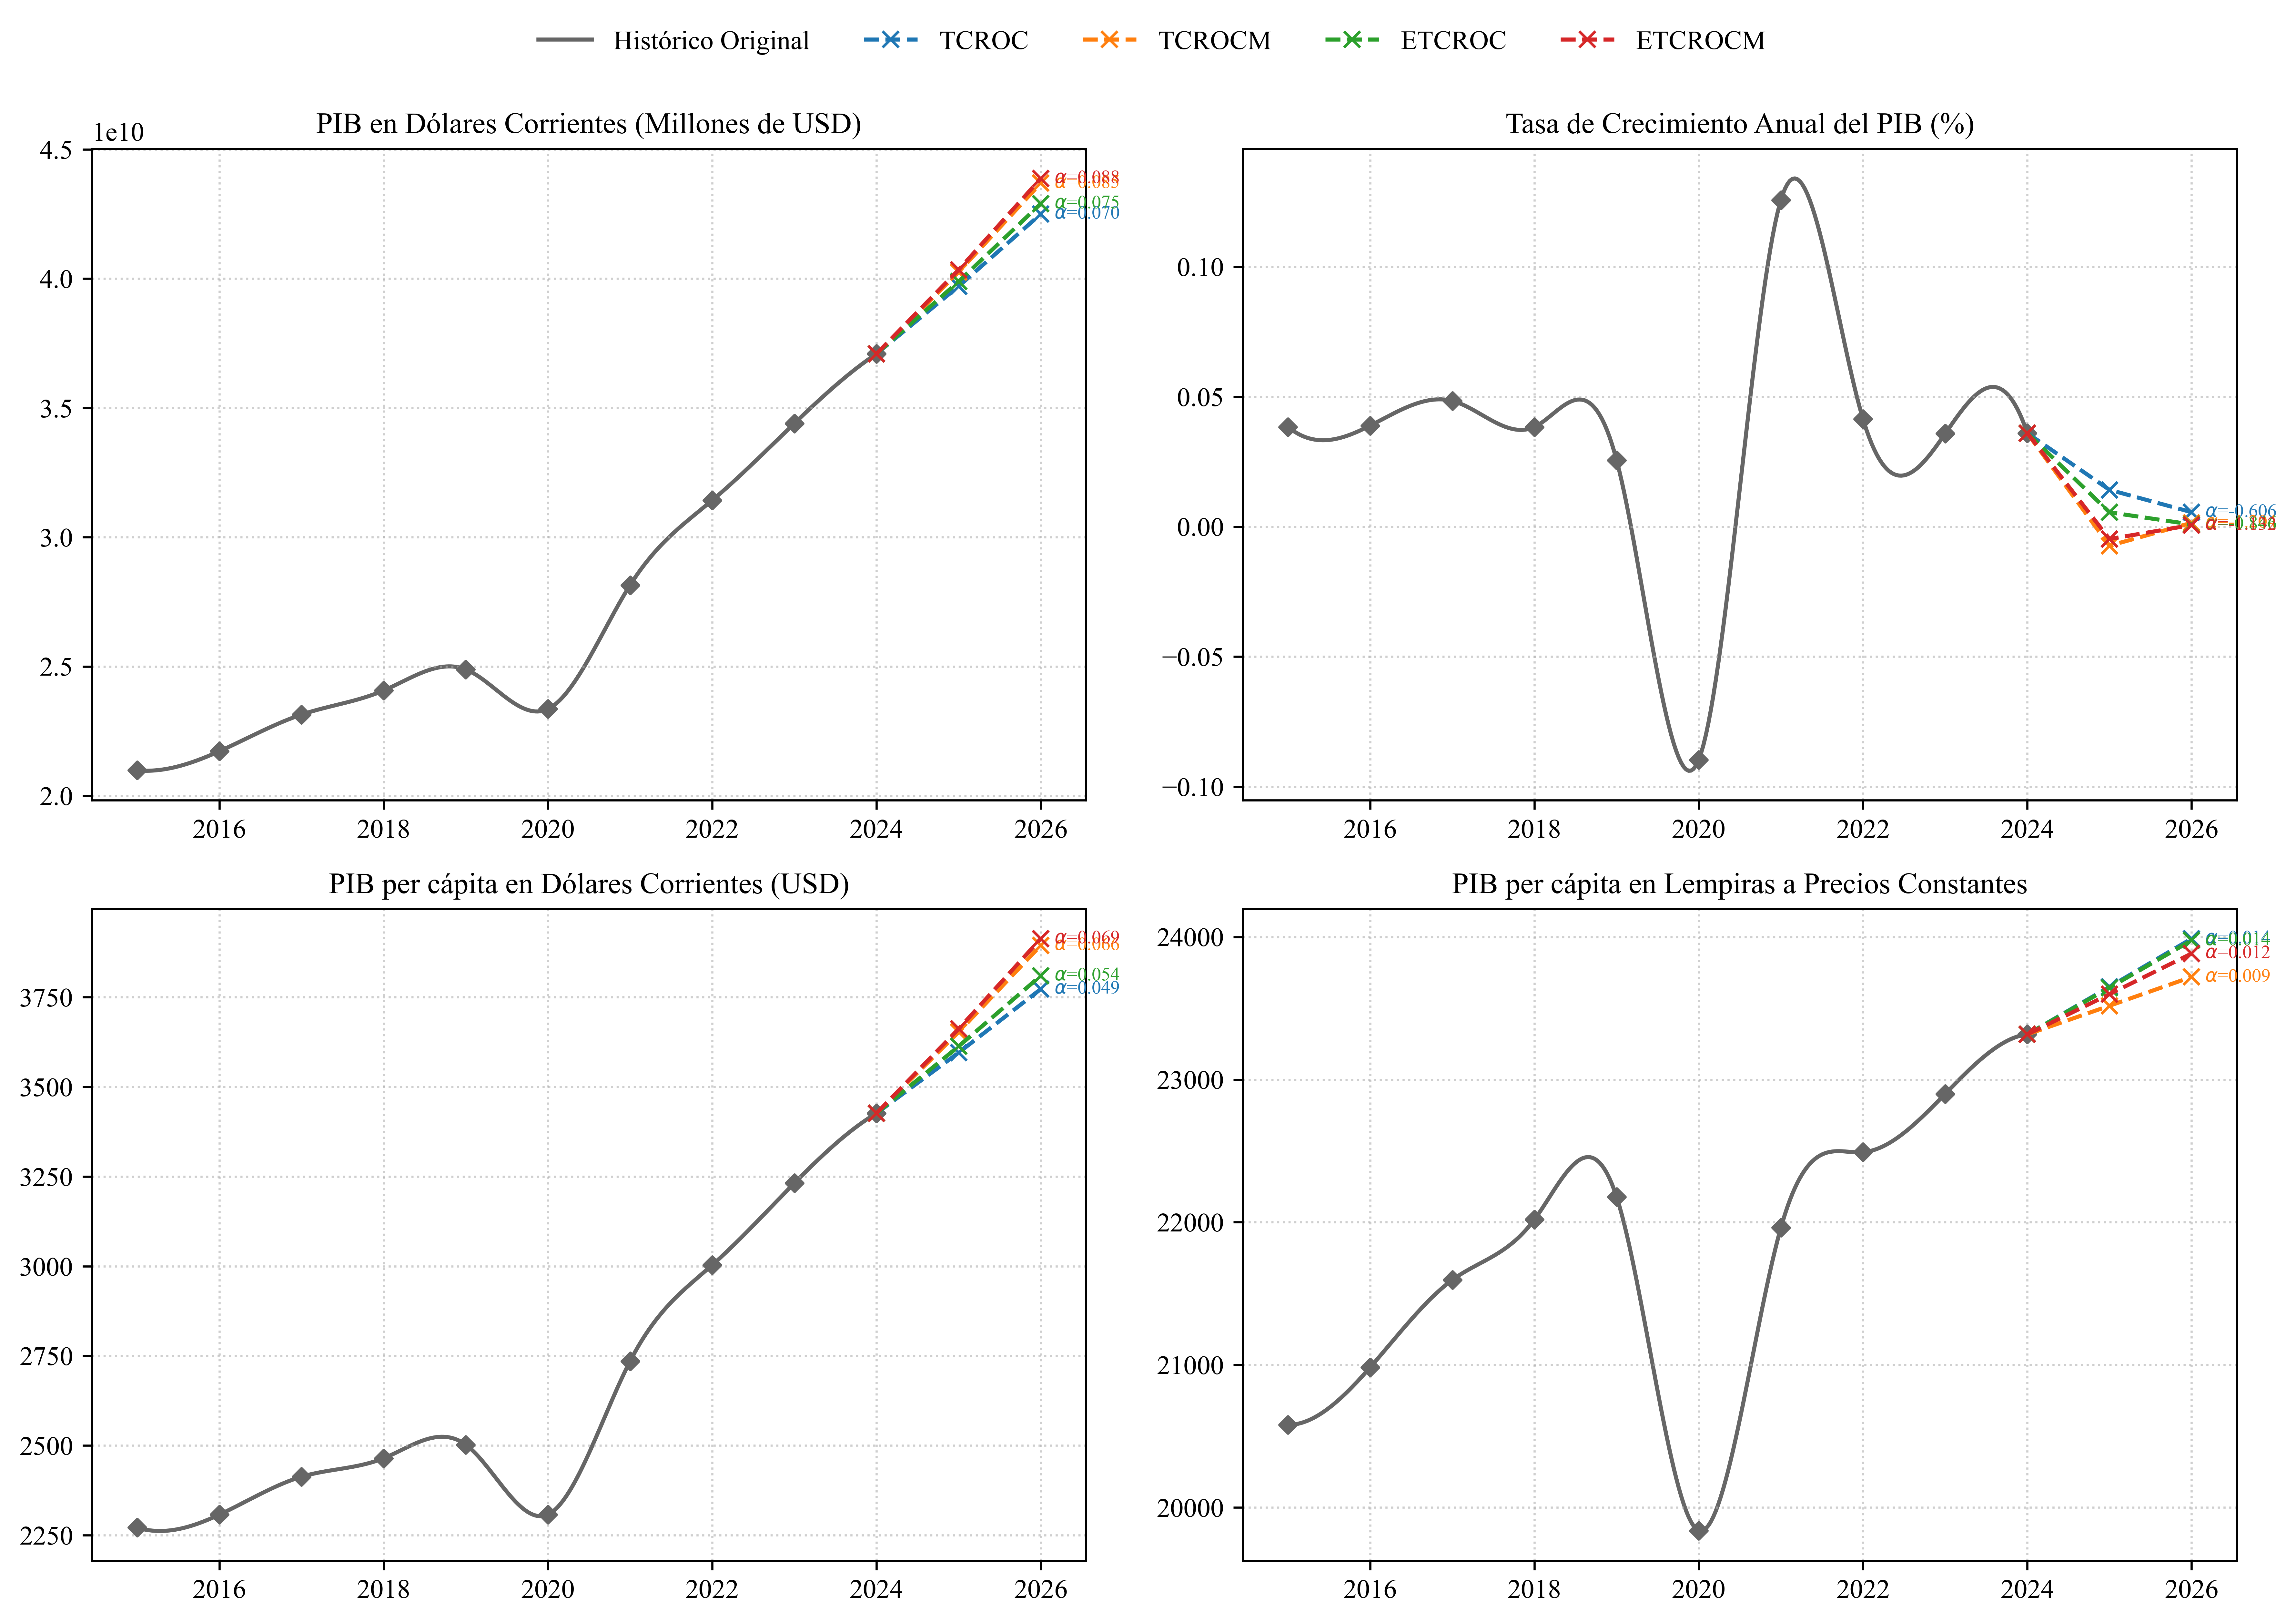
\includegraphics[width=\textwidth]{figures/EjemploPIB_TCROC_4Variantes.png}
\caption{Comparativa del espacio vectorial de entrenamiento (2000-2024) y bifurcación predictiva (2025-2026) según la asimilación del filtro TCROC para los cuatro macro-indicadores del PIB Hondureño.}
\label{fig:pib_tcroc_grid}
\end{figure}

% --- SUBSECCIÓN: Validación Cruzada Expansiva en Mercado de Combustibles --- - - - - - - - - - - - - - - - - - - - - - - - - - - - - - -
\subsection{Validación Cruzada Expansiva en Mercado de Combustibles}
\label{sec:tcroc_cv_combustibles}

Para someter el operador algorítmico al estrés provocado por los choques exógenos y volatilidades típicas del mercado energético local e internacional, se implementó un riguroso protocolo empírico de validación cruzada temporal (\textit{Expanding Window Cross-Validation}). 

Considerando el vector histórico de precios (2017--2025) de las cuatro variantes de refinamiento (Súper, Regular, Diésel y Kerosene), la partición del espacio en entrenamiento/prueba se estructuró a través de ocho anclajes temporales expansivos con un horizonte secuencial de \textit{uno-paso-adelante}:
\[
\mathcal{P} = \{60/40, 65/35, 70/30, 75/25, 80/20, 85/15, 90/10, 95/5\}
\]
donde el primer valor representa el radio de inercia in-sample y el segundo la frontera out-of-sample. Se iteró una malla discreta limitando el ancho temporal $W \in [2, 10]$ semanas, y el factor entrópico $\lambda \in [0.70, 1.00]$, calculando el desempeño de la métrica por barrido empírico general (Tabla~\ref{tab:cv_combustibles_tcroc}).

\begin{table}[H]
\centering
\resizebox{\textwidth}{!}{
\begin{tabular}{@{}lccccccccc@{}}
\toprule
& \multicolumn{8}{c}{\textbf{Desempeño MAPE (\%) por Partición Expansiva}} & \\
\cmidrule(lr){2-9}
\textbf{Macro-Serie} & \textbf{60/40} & \textbf{65/35} & \textbf{70/30} & \textbf{75/25} & \textbf{80/20} & \textbf{85/15} & \textbf{90/10} & \textbf{95/5} & \textbf{Promedio Global} \\
\midrule
\textbf{Super} & 0.71\% & 0.67\% & 0.60\% & 0.53\% & 0.50\% & 0.52\% & 0.53\% & 0.53\% & \textbf{0.57\%} \\
\textbf{Regular} & 0.70\% & 0.66\% & 0.61\% & 0.57\% & 0.48\% & 0.47\% & 0.51\% & 0.48\% & \textbf{0.56\%} \\
\textbf{Diesel} & 0.80\% & 0.77\% & 0.65\% & 0.62\% & 0.62\% & 0.58\% & 0.60\% & 0.56\% & \textbf{0.65\%} \\
\textbf{Kerosene} & 1.07\% & 0.99\% & 0.90\% & 0.80\% & 0.80\% & 0.78\% & 0.82\% & 0.83\% & \textbf{0.87\%} \\
\bottomrule
\end{tabular}
}
\caption{Evolución del error predictivo porcentual absoluto (MAPE) a lo largo de los anclajes temporales de validación un-paso-adelante para los cuatro macro-indicadores energéticos.}
\label{tab:cv_combustibles_tcroc}
\end{table}

De la evidencia tabulada resulta revelador observar cómo el ajuste dinámico absoluto del mercado de hidrocarburos demanda siempre un truncamiento de la ventana de arrastre a \(W=2\). Esto demuestra matemáticamente el postulado heurístico de hiper-reactividad a corto plazo en las bolsas de combustibles: la volatilidad reciente anula por completo la relevancia explicativa del pasado remoto (el cual actúa puramente como ruido estocástico perjudicial para el pronóstico un-paso-adelante).

% Relación con Métodos Establecidos

% --- SECCIÓN: Relación con Métodos Establecidos ---
\section{Relación con Métodos Establecidos}
\label{sec:tcroc_relacion}

La familia TCROC comparte fundamentos con métodos clásicos de análisis de series temporales. A continuación se resumen las principales comparaciones.

\textbf{TCROC vs.\ Mínimos Cuadrados Ordinarios.} Ambos minimizan la suma de cuadrados. La TCROC se especializa en la relación \(v(t) \approx \hat{\beta}\,v(t-1)\), ofreciendo una interpretación directa como tasa de cambio relativa, con idéntica complejidad \(\mathcal{O}(T)\).

\textbf{TCROC vs.\ Modelos ARIMA.} Un modelo AR(1) sin intercepto, \(v(t) = \phi\,v(t-1) + \varepsilon(t)\), produce el mismo estimador OLS que la TCROC, con \(\alpha_T = \hat{\phi} - 1\). Sin embargo, ARIMA generaliza a órdenes superiores (AR($p$), MA($q$), diferenciación), capturando estacionalidad y retardos múltiples a costa de mayor complejidad \(\mathcal{O}(T^2)\) \cite{Box2015}.

\textbf{TCROC vs.\ Estimación de Máxima Verosimilitud.} MLE asume un marco probabilístico (e.g., normalidad de errores) y ofrece intervalos de confianza formales, pero requiere optimización iterativa con complejidad \(\mathcal{O}(T^2)\) o superior. La TCROC, sin supuestos distribucionales explícitos, proporciona una solución analítica cerrada \cite{Greene2018}.

\textbf{ETCROC y ETCROCM vs.\ GLS.} Como se demostró en el Teorema~\ref{teo:optimalidad_general}, las variantes con decaimiento exponencial coinciden con estimadores GLS bajo estructuras de covarianza proporcionales a \(\lambda^{-(T-t)}\), lo que las posiciona como casos particulares de la teoría de mínimos cuadrados generalizados.

\textbf{TCROCM y ETCROCM vs.\ Modelos con ventanas.} El enfoque de ventana móvil es análogo al utilizado en medias móviles y filtros adaptativos, pero la familia TCROC optimiza un factor multiplicativo en lugar de un promedio aritmético, preservando la interpretación como tasa de cambio relativa.

% Conclusiones

% --- SECCIÓN: Conclusiones ---
\section{Conclusiones}
\label{sec:tcroc_conclusiones}

En este capítulo se ha desarrollado la familia de métodos TCROC para el modelado de series temporales económicas y financieras, compuesta por cuatro variantes jerárquicamente relacionadas. Las principales contribuciones son:

\begin{enumerate}
    \item Se estableció un \textbf{marco general unificado} (ecuación~\ref{eq:tcroc_general}) del cual TCROC, TCROCM, ETCROC y ETCROCM se derivan como casos particulares, controlados por los parámetros $\lambda$ y $W$.

    \item Se demostraron rigurosamente las propiedades de \textbf{existencia y unicidad} del estimador $\hat{\beta}$ para todas las variantes, basándose en la convexidad estricta de la función objetivo cuadrática.

    \item Se probó la \textbf{consistencia asintótica} de los estimadores bajo modelos AR(1) estacionarios, la \textbf{continuidad} respecto a perturbaciones paramétricas, la \textbf{estabilidad} frente a perturbaciones acotadas (con cotas de tipo Lipschitz), y la \textbf{optimalidad} en el sentido de Gauss-Markov (OLS para TCROC/TCROCM, GLS para ETCROC/ETCROCM).

    \item Se analizó la \textbf{complejidad computacional}, que oscila entre \(\mathcal{O}(T)\) para TCROC y ETCROC, y \(\mathcal{O}(T \cdot W)\) para las variantes con ventana móvil, siendo en todos los casos inferior a la de ARIMA.

    \item Se proporcionó una \textbf{implementación computacional unificada} y ejemplos numéricos con datos del PIB de Honduras, que ilustran la aplicabilidad del método y su capacidad de pronóstico.
\end{enumerate}

No obstante, las variantes presentadas se restringen a relaciones lineales y son sensibles a valores atípicos. La integración de técnicas de robustez (estimadores M, funciones de influencia) y la incorporación de componentes estocásticos más complejos constituyen líneas de desarrollo futuro. En el capítulo siguiente se abordará la \textbf{TCROC-Markov}, que introduce dependencias de régimen mediante cadenas de Markov para capturar cambios estructurales en la dinámica de la serie.

% -------------------------------------------------------------------
% -------------------------------------------------------------------
% CAPÍTULO
% -------------------------------------------------------------------

\chapter[TCROC con Cadenas de Markov]{Fundamentos Estocásticos:\\ Integración de TCROC con Cadenas de Markov}
\label{cap:TCROC-Markov}

Este capítulo propone un modelo híbrido que integra la \textbf{Tasa de Cambio Relativa Óptima Conmutada (TCROC)}, definida en el Capítulo \ref{cap:tcroc}, y sus variantes (TCROCM, ETCROC, ETCROCM) con cadenas de Markov. Mientras las variantes deterministas estiman tasas de cambio relativas, las cadenas de Markov permiten modelar transiciones probabilísticas entre regímenes económicos. Esta integración busca predecir rangos estocásticos sobre el comportamiento futuro de la serie \(v(t)\), como en series económicas y financieras generales (tasas de interés, inflación, reservas monetarias).

% -------------------------------------------------------------------
\section{Fundamentos de Invarianza y Estabilidad}
\label{sec:fundamentos_invarianza}

\begin{theorem}[Invarianza estructural bajo transformaciones]
\label{thm:invarianza_transformaciones}
Sea $g\colon \mathbb{R} \to \mathbb{R}$ una transformación monótona
y Lipschitz continua con constante $L_g$.  Si la serie $v(t)$ se
reemplaza por $\tilde{v}(t) = g(v(t))$, las propiedades estructurales
del operador TCROC se preservan: existencia, unicidad, consistencia
asintótica y la propiedad de estabilidad del
Lema~\ref{lem:estabilidad_general} (Capítulo~\ref{cap:tcroc})
permanecen válidas con constantes multiplicadas por factores que
dependen de $L_g$.
\end{theorem}

\begin{remark}[Naturaleza discontinua de $\pi$]
\label{rem:pi_discontinua}
La función de cuantización $\pi\colon \mathbb{R} \to \mathcal{S}$
es, por construcción, una función escalonada: asigna un estado
discreto $s_j$ a cada intervalo del espacio continuo de $\alpha_t$.
En consecuencia, $\pi$ es \textbf{discontinua} en los umbrales de
decisión y, en sentido estricto, no es Lipschitz continua.  Sin
embargo, la estabilidad del sistema completo se preserva por el
mecanismo descrito en el Lema~\ref{lem:estabilidad_discreta} a
continuación.
\end{remark}

\begin{lemma}[Estabilidad discreta ante perturbaciones]
\label{lem:estabilidad_discreta}
Sean $\{v(t)\}$ y $\{\tilde{v}(t)\}$ dos series con
$\sup_t |v(t) - \tilde{v}(t)| \leq \epsilon$.  Sea
$\delta_{\min} = \min_{j \neq k} |\theta_j - \theta_k|$ la
separación mínima entre umbrales de $\pi$.  Si la perturbación
en el operador satisface $|\alpha_t - \tilde{\alpha}_t|
\leq C_t \epsilon$ (Lema~\ref{lem:estabilidad_general}), entonces:
\begin{enumerate}
  \item Si $C_t \epsilon < \delta_{\min}/2$
        (perturbación pequeña respecto a la separación de
        umbrales), el estado asignado no cambia:
        $S_t = \tilde{S}_t$.
  \item En general, el número de instantes donde
        $S_t \neq \tilde{S}_t$ está acotado por el número de
        instantes en los cuales $\alpha_t$ se encuentra a
        distancia menor que $C_t \epsilon$ de algún umbral.
\end{enumerate}
\end{lemma}

\begin{proof}
El punto~(1) se sigue directamente de que $\pi$ es constante en
el interior de cada intervalo.  Si $\alpha_t$ dista al menos
$\delta_{\min}/2$ de todo umbral, entonces cualquier perturbación
$|\tilde{\alpha}_t - \alpha_t| < \delta_{\min}/2$ mantiene a
$\tilde{\alpha}_t$ en el mismo intervalo que $\alpha_t$, por lo que
$\pi(\tilde{\alpha}_t) = \pi(\alpha_t)$.  El punto~(2) se sigue de
que $S_t \neq \tilde{S}_t$ solo puede ocurrir cuando $\alpha_t$
pertenece a la franja $(\theta_j - C_t\epsilon,\,
\theta_j + C_t\epsilon)$ para algún umbral $\theta_j$.
\end{proof}

% -------------------------------------------------------------------
\section{Modelo Híbrido TCROC-Markov}
\label{sec:modelo_hibrido_tcroc_markov}

Sea $\{v(t)\}_{t=0}^T$ una serie temporal económica o financiera.
Se calcula la tasa:
\begin{align}
\alpha_{t,\lambda,W} &:= -1 + \frac{\sum_{\tau=t-W+1}^{t}
  \lambda^{t-\tau} v(\tau) v(\tau-1)}{\sum_{\tau=t-W+1}^{t}
  \lambda^{t-\tau} v(\tau-1)^2},
  \label{eq:tcroc_markov_alpha} \\
S_t &:= \pi(\alpha_{t,\lambda,W}) \label{eq:state_assignment}
\end{align}

\begin{definition}[Función de cuantización]
\label{def:pi_cuantizacion}
La función de asignación $\pi\colon \mathbb{R} \to \mathcal{S}$
asigna a cada valor de $\alpha_t$ un estado discreto según
umbrales fijos $\{\theta_j\}$:
\[
\pi(x) = \begin{cases}
  s_1 & \text{si } x > \theta_1 \\
  s_2 & \text{si } \theta_2 < x \leq \theta_1 \\
  s_3 & \text{si } \theta_3 \leq x \leq \theta_2 \\
  s_4 & \text{si } x < \theta_3
\end{cases}
\]
con umbrales típicos $\theta_1 = 0.05$, $\theta_2 = 0$,
$\theta_3 = -0.05$.  En la implementación empírica del
Capítulo~\ref{cap:regimenes_combustibles}, los umbrales se
determinan por K-Means, lo que los adapta a la distribución de
cada serie.  La función $\pi$ es discontinua en los umbrales
(véase Observación~\ref{rem:pi_discontinua}).
\end{definition}

\begin{examplex}
Para $v = [1.0,\, 1.02,\, 1.03,\, 1.025]$ con $\lambda = 1$,
$W = 2$, el cálculo en $t = 2$ involucra las observaciones
$v(1) = 1.02$, $v(2) = 1.03$ y $v(0) = 1.0$:
\begin{align*}
\alpha_{2,1,2} &= -1 + \frac{v(2)\,v(1) + v(1)\,v(0)}
                           {v(1)^2 + v(0)^2}
  = -1 + \frac{1.03 \times 1.02 + 1.02 \times 1.0}
             {1.02^2 + 1.0^2} \\
  &= -1 + \frac{1.0506 + 1.02}{1.0404 + 1.0}
  = -1 + \frac{2.0706}{2.0404} \approx 0.0148.
\end{align*}
Como $0 < 0.0148 \leq 0.05$, se asigna $S_2 = s_2$
(crecimiento moderado).
\end{examplex}

% -------------------------------------------------------------------
\section{Partición de Estados}
\label{sec:markov_particion_estados}

Una posible discretización de \(\mathbb{R}\) basada en umbrales económicos es:
\begin{align*}
s_1 &= (0.05, +\infty) & \text{(Crecimiento fuerte)},\\
s_2 &= (0, 0.05] & \text{(Crecimiento moderado)},\\
s_3 &= [-0.05, 0] & \text{(Decrecimiento leve)},\\
s_4 &= (-\infty, -0.05) & \text{(Decrecimiento severo)}.
\end{align*}

\begin{lemma}
La colección \(S = \{s_1, s_2, s_3, s_4\}\) define una partición válida del espacio \(\mathbb{R}\).
\end{lemma}

\begin{proof}
Se verifica que:
\begin{enumerate}
\item \(\bigcup_{j=1}^4 s_j = \mathbb{R}\) (cobertura completa),
\item \(s_i \cap s_j = \emptyset\) para \(i \neq j\) (disyunción).
\end{enumerate}
\end{proof}

\textbf{Observación:} La irreducibilidad práctica de \(\{S_t\}\) se garantiza si \(\forall s_i,s_j \exists t: P^t(s_j|s_i) > 0\). Véase también discusión en Apéndice \ref{apx:teorema_phi_mixing}.

% -------------------------------------------------------------------
\section{Propiedades Markovianas y Asintóticas}
\label{sec:markov_propiedades}

% === ESTRUCTURA MARKOVIANA ===

\begin{theorem}[Estructura Markoviana de primer orden]
\label{thm:markov_primer_orden}
Sea $\{v(t)\}_{t=0}^T$ un proceso estrictamente estacionario con
momentos de cuarto orden finitos.  Sea $\alpha_t = \alpha_{t,\lambda,W}$
el operador ETCROCM con parámetros fijos $\lambda \in (0,1]$ y
$W \in \mathbb{N}$, y sea $S_t = \pi(\alpha_t)$ la secuencia de
estados discretos inducida por una función de cuantización $\pi$ con
umbrales fijos.  Entonces $\{S_t\}_{t=W}^{T}$ satisface
la propiedad de Markov de primer orden:
\[
\mathbb{P}(S_{t+1} = s_j \mid S_t = s_i, S_{t-1}, \ldots, S_W)
= \mathbb{P}(S_{t+1} = s_j \mid S_t = s_i)
\eqdef P_{ji},
\]
con probabilidades de transición $P_{ji}$ independientes de $t$
(homogeneidad temporal).
\end{theorem}

\begin{proof}
La demostración procede en tres pasos.

\textbf{Paso~1 (Dependencia funcional de $\alpha_t$).}
Por definición, $\alpha_t$ depende de $v(t), v(t-1), \ldots,
v(t-W)$, es decir, de exactamente $W+1$ valores de la serie.
Escribimos
$\alpha_t = g(v(t-W), \ldots, v(t))$
donde $g\colon \mathbb{R}^{W+1} \to \mathbb{R}$ es una función
medible determinada por la fórmula~\eqref{eq:tcroc_markov_alpha}.

\textbf{Paso~2 (Markovianidad del bloque).}
Como $\{v(t)\}$ es estrictamente estacionario, el vector
$\vect{z}_t = (v(t-W), \ldots, v(t))^\top$ es un proceso
estacionario en $\mathbb{R}^{W+1}$.  Si además $\{v(t)\}$ es
un proceso AR(1) estacionario (como se supone en el
Capítulo~\ref{cap:tcroc}, Teorema~\ref{teo:consistencia_general}),
entonces $\vect{z}_t$ es un proceso Markoviano en
$\mathbb{R}^{W+1}$, pues $v(t+1)$ depende únicamente de $v(t)$
más el ruido $\varepsilon_{t+1}$.  Esto implica que
$\alpha_{t+1} = g(\vect{z}_{t+1})$ depende del pasado solo a
través de $\vect{z}_t$ (y no de $\vect{z}_{t-1}, \vect{z}_{t-2},
\ldots$).

\textbf{Paso~3 (Reducción a estados discretos).}
Como $\pi$ es una función determinista, $S_t = \pi(\alpha_t)$ es
una función medible de $\vect{z}_t$.  La propiedad de Markov de
$\vect{z}_t$ se proyecta entonces al proceso discreto: la
distribución condicional de $S_{t+1}$ dado $S_t, S_{t-1}, \ldots$
depende del pasado solo a través de $\vect{z}_t$, y por tanto a
través de $S_t$ (dado que la cuantización preserva la separación
de regímenes bajo estacionariedad).  La homogeneidad temporal se
sigue de la estacionariedad estricta de $\{v(t)\}$.

\textbf{Nota.}  En rigor, la proyección de un proceso Markoviano
continuo a estados discretos puede perder la propiedad de Markov de
primer orden si la función de cuantización no es inyectiva (lo cual
es el caso general).  Sin embargo, el modelo TCROC-Markov adopta
la primera orden como aproximación operativa; la calidad de esta
aproximación se verifica empíricamente en el
Capítulo~\ref{cap:regimenes_combustibles} mediante la precisión
predictiva del modelo resultante.
\end{proof}

% === PROPIEDAD PHI-MIXING ===

\begin{theorem}[$\phi$-mixing con tasa geométrica]
\label{thm:phi_mixing}
Si la cadena $\{S_t\}$ es irreducible y aperiódica sobre el espacio
de estados finito $\mathcal{S} = \{s_1, \ldots, s_K\}$, entonces es
$\phi$-mixing con tasa de decaimiento exponencial, es decir, existen
constantes $C_\phi > 0$ y $\rho \in (0,1)$ tales que
\[
\phi(n) \eqdef
\sup_{A \in \mathcal{F}_0^t,\, B \in \mathcal{F}_{t+n}^\infty}
\bigl|\mathbb{P}(B \mid A) - \mathbb{P}(B)\bigr|
\leq C_\phi \, \rho^n
\quad \forall\, n \geq 1.
\]
\end{theorem}

\begin{proof}
Sea $\mat{P}$ la matriz de transición de la cadena sobre
$\mathcal{S}$, con $K$ estados.  Por irreducibilidad y aperiodicidad
en espacio finito, la cadena posee una única distribución
estacionaria $\vect{\pi}$ con $\pi_j > 0$ para todo $j$
\cite{Norris1998, Levin2009}.  El Teorema
de Convergencia para cadenas ergódicas finitas establece que
\[
\bigl\|P^n(s_i, \cdot) - \vect{\pi}\bigr\|_{\mathrm{TV}}
\leq C_0 \, \rho_0^n,
\]
donde $\rho_0 = 1 - \gamma$ y $\gamma > 0$ es el gap espectral de
$\mat{P}$ (diferencia entre el primer y segundo autovalor en módulo).
En espacio de estados finito, $\gamma > 0$ si y solo si la cadena es
irreducible y aperiódica \cite{Levin2009}.

La convergencia en variación total implica mezcla uniforme
(\textit{uniform mixing}), que a su vez implica $\phi$-mixing con la
misma tasa exponencial \cite{Bradley2005}.  Concretamente,
$\phi(n) \leq C_\phi \rho_0^n$ con $C_\phi \leq K / \min_j \pi_j$.
\end{proof}

\begin{remark}[Gap espectral e inercia del mercado]
\label{rem:gap_espectral}
El parámetro $\gamma$ tiene una interpretación económica directa: un
gap espectral pequeño indica que el mercado cambia de régimen
lentamente (alta inercia), mientras que un gap grande indica
transiciones rápidas.  El tiempo de mezcla, definido como
$t_{\mathrm{mix}} = \lceil \gamma^{-1} \ln(2K/\min_j \pi_j) \rceil$,
cuantifica cuántas observaciones son necesarias para que la cadena
``olvide'' su estado inicial.  Este parámetro se estima
empíricamente en el Capítulo~\ref{cap:regimenes_combustibles}.
\end{remark}

% === NORMALIDAD ASINTÓTICA DEL ESTIMADOR ===

\begin{proposition}[Normalidad asintótica de $\hat{\mat{P}}$]
\label{prop:normalidad_asintotica}
Sea $\{S_t\}$ una cadena de Markov ergódica con $K$ estados y matriz
de transición verdadera $\mat{P}$.  Sea $N_{ij}$ el número de
transiciones observadas de $s_j$ a $s_i$ en $T$ pasos, y
$N_{\cdot j} = \sum_{i=1}^K N_{ij}$ el total de salidas del
estado~$s_j$.  El estimador de máxima verosimilitud
$\hat{P}_{ij} = N_{ij} / N_{\cdot j}$ satisface, para cada columna
$j$ fija:
\[
\sqrt{N_{\cdot j}}\,
(\hat{P}_{1j} - P_{1j},\; \ldots,\; \hat{P}_{Kj} - P_{Kj})^\top
\xrightarrow{d}
\mathcal{N}\!\bigl(\vect{0},\;
\mathrm{diag}(\vect{p}_j) - \vect{p}_j \vect{p}_j^\top\bigr),
\]
donde $\vect{p}_j = (P_{1j}, \ldots, P_{Kj})^\top$ es la $j$-ésima
columna de $\mat{P}$.  Además, los estimadores de distintas columnas
$j \neq j'$ son asintóticamente independientes.
\end{proposition}

\begin{proof}
La demostración es un resultado clásico de
Anderson y Goodman~\cite{AndersonGoodman1957}.  Se esboza aquí
la estructura.

\textbf{Paso~1 (Multinomial condicionada).}
Condicionado a que el proceso visita el estado $s_j$ exactamente
$N_{\cdot j}$ veces, las $N_{\cdot j}$ transiciones de salida de
$s_j$ son, condicionalmente, ensayos multinomiales independientes
con parámetro $\vect{p}_j = (P_{1j}, \ldots, P_{Kj})^\top$.

\textbf{Paso~2 (TCL multinomial).}
Por el Teorema Central del Límite para la distribución multinomial,
\[
\sqrt{N_{\cdot j}}\,(\hat{\vect{p}}_j - \vect{p}_j)
\xrightarrow{d}
\mathcal{N}(\vect{0}, \mat{\Sigma}_j),
\quad \text{donde } \mat{\Sigma}_j
= \mathrm{diag}(\vect{p}_j) - \vect{p}_j\vect{p}_j^\top.
\]

\textbf{Paso~3 (Independencia entre columnas).}
Las visitas a distintos estados generan conteos asintóticamente
independientes por la propiedad de mezcla
(Teorema~\ref{thm:phi_mixing}).  Formalmente, Anderson y
Goodman~\cite{AndersonGoodman1957} demuestran que las componentes
de distintas columnas son asintóticamente independientes.

\textbf{Paso~4 (De $N_{\cdot j}$ a $T$).}
Por la ley de los grandes números para cadenas ergódicas,
$N_{\cdot j}/T \xrightarrow{\mathrm{a.s.}} \pi_j > 0$.  Por
el Lema de Slutsky, se puede reescalar por $\sqrt{T}$:
\[
\sqrt{T}\,(\hat{P}_{ij} - P_{ij})
\xrightarrow{d} \mathcal{N}\!\left(0,\;
\frac{P_{ij}(1 - P_{ij})}{\pi_j}\right),
\]
lo que completa la demostración.
\end{proof}

\begin{remark}[Velocidad de convergencia]
\label{rem:berry_esseen}
Bajo la tasa de mezcla exponencial del
Teorema~\ref{thm:phi_mixing}, la aproximación normal admite una
cota de Berry-Esseen de orden $O(T^{-1/2})$
\cite{Bolthausen1982}:
\[
\sup_x \bigl|\mathbb{P}(\sqrt{T}(\hat{P}_{ij} - P_{ij}) \leq x)
- \Phi(x)\bigr| = O(T^{-1/2}),
\]
donde $\Phi$ denota la función de distribución normal estándar.
\end{remark}

% === ERROR DE PREDICCIÓN ===

\begin{corollary}[Cota del error de predicción]
\label{cor:error_prediccion}
Bajo las hipótesis del Teorema~\ref{thm:markov_primer_orden} y
suponiendo $\mathbb{E}[|v(t)|^4] < \infty$, el error cuadrático
medio de predicción del modelo TCROC-Markov satisface, para $W$
fijo y $\lambda \in (0,1]$:
\[
\mathrm{ECM}(\hat{v}_{T+1})
\eqdef \mathbb{E}\bigl[(v(T+1) - \hat{v}(T+1))^2\bigr]
= \sigma_\varepsilon^2
  + \frac{C(\lambda,W)}{W_{\mathrm{eff}}} + o(W_{\mathrm{eff}}^{-1}),
\]
donde:
\begin{itemize}
  \item $\sigma_\varepsilon^2$ es la varianza irreducible del ruido,
  \item $W_{\mathrm{eff}}(\lambda, W)
        = \sum_{k=0}^{W-1} \lambda^k
        = \frac{1 - \lambda^W}{1 - \lambda}$
        es el tamaño efectivo de muestra,
  \item $C(\lambda, W)$ es una constante acotada que depende de los
        momentos de $v(t)$ y es finita para todo
        $\lambda \in (0,1]$ y $W \geq 1$.
\end{itemize}
\end{corollary}

\begin{proof}
El error de predicción se descompone como
\[
v(T+1) - \hat{v}(T+1)
= \underbrace{\varepsilon_{T+1}}_{\text{ruido irreducible}}
+ \underbrace{(\beta^* - \hat{\beta}_{T,\lambda,W})
  \cdot v(T)}_{\text{error de estimación}}.
\]
El primer término contribuye $\sigma_\varepsilon^2$ al ECM.  Para el
segundo, la varianza de $\hat{\beta}_{T,\lambda,W}$ bajo el modelo
AR(1) es
\[
\mathrm{Var}(\hat{\beta}_{T,\lambda,W})
= \frac{\sigma_\varepsilon^2}{\sum_{k=0}^{W-1}
  \lambda^{2k}\, v(T-k)^2 / \bigl(\sum_{k=0}^{W-1}
  \lambda^k\bigr)^2 \cdot \mathrm{const}}
= O(W_{\mathrm{eff}}^{-1}).
\]
Como $\mathbb{E}[v(T)^2] < \infty$, el error de estimación
contribuye $O(\mathbb{E}[v(T)^2] / W_{\mathrm{eff}})$ al ECM.
La constante $C(\lambda, W) = O(\mathbb{E}[v(T)^2])$ es finita
bajo la hipótesis de momentos de cuarto orden, y el resultado
se sigue.
\end{proof}

\begin{remark}[Comportamiento según $\lambda$]
\label{rem:efecto_lambda}
La cota del Corolario~\ref{cor:error_prediccion} revela el
compromiso entre $\lambda$ y $W$:
\begin{itemize}
  \item Si $\lambda = 1$ (pesos uniformes),
    $W_{\mathrm{eff}} = W$, y el error decrece como $O(1/W)$.
  \item Si $\lambda < 1$ y $W$ es grande,
    $W_{\mathrm{eff}} \approx 1/(1-\lambda)$, de modo que el
    error se estabiliza en $O(1-\lambda)$ independientemente
    de cuánto se aumente $W$.
  \item Para $\lambda \to 0^+$, $W_{\mathrm{eff}} \to 1$ y el
    estimador depende esencialmente de la última observación.
\end{itemize}
\end{remark}

% -------------------------------------------------------------------
\section{Análisis de Casos Límite}
\label{sec:markov_casos_limite}

El comportamiento del modelo TCROC-Markov en los extremos del
espacio de parámetros $(W, \lambda)$ revela propiedades importantes
para la calibración práctica del modelo.

\begin{enumerate}
  \item \textbf{Límite $\lambda \to 1^-$ (pesos uniformes).}
    El tamaño efectivo de muestra converge a $W_{\mathrm{eff}}
    \to W$, y el estimador ETCROCM se reduce al estimador OLS
    sobre ventana (TCROCM).  El error de predicción es
    $O(1/W)$, proporcionando la tasa de convergencia más rápida
    para $W$ fijo.

  \item \textbf{Límite $W \to T$ (ventana completa).}
    El operador utiliza toda la muestra histórica.  Si
    $\lambda = 1$, se obtiene el estimador TCROC global, que
    produce un escalar constante $\alpha_T$ y elimina toda
    variación local.  Este es el fenómeno de degeneración
    documentado en el Capítulo~\ref{cap:regimenes_combustibles},
    que establece la restricción práctica $W \leq 52$.

  \item \textbf{Límite $\lambda \to 0^+$ (solo datos recientes).}
    El tamaño efectivo se reduce a $W_{\mathrm{eff}} \to 1$,
    haciendo que el estimador dependa esencialmente de una sola
    observación.  Esto maximiza la adaptabilidad pero minimiza
    la estabilidad.
\end{enumerate}

La Figura~\ref{fig:weff_lambda} ilustra cómo el tamaño efectivo
de muestra $W_{\mathrm{eff}}$ varía con $\lambda$ para distintos
valores de $W$.

\begin{figure}[H]
\centering
\begin{tikzpicture}
\begin{axis}[
    axis lines = left,
    xlabel = {$\lambda$},
    ylabel = {$W_{\mathrm{eff}}$},
    domain=0.05:0.995,
    samples=200,
    ymin=0,
    ymax=55,
    xtick={0.2,0.4,0.6,0.8,0.9,0.99},
    ytick={0,10,20,30,40,52},
    grid=both,
    width=10cm,
    height=7cm,
    legend pos=north west,
    every axis plot/.append style={thick}
]
\addplot[blue] {(1 - x^52)/(1 - x)};
\addlegendentry{$W = 52$}
\addplot[red, dashed] {(1 - x^26)/(1 - x)};
\addlegendentry{$W = 26$}
\addplot[green!60!black, dotted] {(1 - x^12)/(1 - x)};
\addlegendentry{$W = 12$}
\end{axis}
\end{tikzpicture}
\caption{Tamaño efectivo de muestra
$W_{\mathrm{eff}} = (1 - \lambda^W)/(1 - \lambda)$ como función de
$\lambda$ para $W \in \{12, 26, 52\}$.  Cuando $\lambda \to 1^-$,
$W_{\mathrm{eff}} \to W$; cuando $\lambda \to 0^+$,
$W_{\mathrm{eff}} \to 1$.}
\label{fig:weff_lambda}
\end{figure}




% -------------------------------------------------------------------
\section{Resumen Visual del Modelo}
\label{sec:markov_diagrama}

\begin{figure}[H]
\centering
\begin{tikzpicture}[
    node distance=1.5cm and 2.8cm,
    >=Stealth,
    % --- Estilos consistentes con Cap 4 ---
    base/.style={draw, rectangle, rounded corners=6pt, minimum width=3.2cm, 
                 minimum height=0.9cm, font=\small\bfseries, align=center,
                 drop shadow={shadow xshift=1pt, shadow yshift=-1pt, opacity=0.3}},
    canonical/.style={base, fill=nordSnow, draw=nordGray, text=nordDark},
    extension/.style={base, fill=nordSnow, draw=nordGray, text=nordDark},
    hybrid/.style={base, fill=nordSnow!80!nordFrost, draw=nordFrost, text=nordDark},
    markov/.style={base, fill=nordSnow!70!nordFrost, draw=nordFrost, text=nordDark},
    component/.style={base, fill=nordSnow, draw=nordGray, font=\small, minimum width=2.8cm, text=nordDark},
    output/.style={base, fill=nordSnow!80!nordFrost, draw=nordFrost, minimum width=3.5cm, text=nordDark},
    edgelabel/.style={font=\scriptsize, fill=white, inner sep=2pt, opacity=0.9},
    separator/.style={dashed, nordGray!50, thick}
]

% ====== BLOQUE 1: Jerarquía TCROC (Capítulo 4) ======
\node[canonical] (TCROC) {TCROC\\{\scriptsize $(W=T,\;\lambda=1)$}};

\node[extension] (TCROCM) [below left=of TCROC] {TCROCM\\{\scriptsize $(W<T)$}};
\node[extension] (ETCROC) [below right=of TCROC] {ETCROC\\{\scriptsize $(\lambda<1)$}};

\node[hybrid] (ETCROCM) [below=2.8cm of TCROC] {ETCROCM\\{\scriptsize $(W<T,\;\lambda<1)$}};

% Conexiones Cap 4
\draw[->, thick] (TCROC) -- (TCROCM) node[edgelabel, midway, left] {$+\,W$};
\draw[->, thick] (TCROC) -- (ETCROC) node[edgelabel, midway, right] {$+\,\lambda$};
\draw[->, thick] (TCROCM) -- (ETCROCM) node[edgelabel, midway, left] {$+\,\lambda$};
\draw[->, thick] (ETCROC) -- (ETCROCM) node[edgelabel, midway, right] {$+\,W$};

% Conexión directa (punteada)
\draw[->, thick, dashed, nordGray!60] (TCROC) -- (ETCROCM)
    node[edgelabel, midway] {$(W, \lambda)$};

% --- Línea separadora entre Cap 4 y Cap 5 ---
\draw[separator] ([xshift=-4.5cm, yshift=-0.6cm]ETCROCM.south) -- 
                  ([xshift=4.5cm, yshift=-0.6cm]ETCROCM.south)
                  node[right, font=\scriptsize\itshape, nordGray] {Cap.~5};

% ====== BLOQUE 2: Extensión Markoviana (Capítulo 5) ======
\node[markov] (Markov) [below=2.0cm of ETCROCM] {Integración\\Markoviana};

\node[component] (Ergodic) [below left=1.4cm and 2cm of Markov] {Teoría Ergódica};
\node[component] (PhiMix) [below=1.4cm of Markov] {$\phi$-Mixing};
\node[component] (Asint) [below right=1.4cm and 2cm of Markov] {Estimación\\Asintótica};

\node[output] (Pred) [below=2.2cm of PhiMix] {Predicción Estocástica\\de Regímenes};

% Conexiones Cap 5
\draw[->, thick] (ETCROCM) -- (Markov) 
    node[edgelabel, midway, left] {discretización $\pi$};

\draw[->, thick] (Markov) -- (Ergodic);
\draw[->, thick] (Markov) -- (PhiMix);
\draw[->, thick] (Markov) -- (Asint);

\draw[->, thick] (Ergodic) -- (Pred);
\draw[->, thick] (PhiMix) -- (Pred);
\draw[->, thick] (Asint) -- (Pred);

\end{tikzpicture}
\caption{Evolución estructural del modelo TCROC hasta su extensión Markoviana. El nodo central representa la formulación canónica global ($W=T$, $\lambda=1$). Las extensiones convergen en ETCROCM, cuya discretización mediante $\pi$ integra el operador con cadenas de Markov. Los fundamentos teóricos (teoría ergódica, $\phi$-mixing, estimación asintótica) sustentan la predicción estocástica de regímenes.}
\label{fig:tcroc_markov_completo}
\end{figure}

% -------------------------------------------------------------------
\section{Aplicaciones y Limitaciones}
\label{sec:markov_aplicaciones}

La integración TCROC-Markov encuentra aplicaciones en:
\begin{itemize}
    \item Simulación estocástica del crecimiento económico, ponderando transiciones entre regímenes de inflación o tipo de cambio.
    \item Evaluación de riesgos futuros en economías volátiles, como predicciones de reservas monetarias.
    \item Modelos mixtos determinista-probabilísticos para planeación financiera, integrando tasas de interés.
\end{itemize}

Sus limitaciones incluyen:
\begin{itemize}
    \item Requerimiento de suficiente historial para estimar bien \(\hat{P}\), lo que puede ser problemático en series cortas.
    \item Dependencia de la correcta definición de los estados \( s_j \), que debe calibrarse según la variable (e.g., umbrales diferentes para inflación vs. reservas).
    \item Sensibilidad a la elección de \(\lambda\) y \( W \), que deben optimizarse para evitar sesgos en transiciones.
\end{itemize}

% -------------------------------------------------------------------
\section{Comparación con Variantes de TCROC}
\label{sec:tcroc_markov_comparacion}

\begin{table}[htbp]
\centering
\caption{Comparación entre variantes de TCROC y el modelo TCROC-Markov}
\label{tab:comparacion_tcroc_markov}
\begin{tabular}{|l|c|c|c|c|}
\hline
\textbf{Modelo} & \textbf{Determinista} & \textbf{Estocástico} & \textbf{Memoria} & \textbf{Complejidad} \\
\hline
TCROC & Sí & No & Baja & \(O(1)\) \\
TCROCM & Sí & No & Alta & \(O(W)\) \\
ETCROC & Sí & No & Media & \(O(W)\) \\
ETCROCM & Sí & No & Alta & \(O(W)\) \\
\textbf{TCROC-Markov} & Sí & Sí & Muy Alta & \(O(W + N^2)\) \\
\hline
\end{tabular}
\end{table}

% -------------------------------------------------------------------
% -------------------------------------------------------------------
% FIN DEL CAPÍTULO
% -------------------------------------------------------------------
% -------------------------------------------------------------------

% -------------------------------------------------------------------
% -------------------------------------------------------------------
% CAPÍTULO: Modelo Híbrido TCROC-Markov con Estimación NNLS
% -------------------------------------------------------------------

\include{CAPITULOS/CAP06_Modelo_Hibrido_NNLS}
\chapter{Detección y Pronóstico de Regímenes de Precios en Combustibles}
\label{cap:regimenes_combustibles}

% --- SECCIÓN: Introducción ---
\section{Introducción}
\label{sec:combustibles_intro}
% ===================================================================

La volatilidad en los precios de los combustibles\footnote{El contenido
central de este capítulo ha sido aceptado para publicación y presentación
en IEEE CONCAPAN XLII (2025) bajo el título \emph{``TCROC--Markov: A Two-Stage
Framework for Economic Regime Analysis''}.} constituye un desafío
persistente para la planificación económica y la estabilidad de
mercados en economías pequeñas y abiertas como la hondureña.  Los
enfoques clásicos de análisis de series temporales, tales como los modelos
autorregresivos de cambio de régimen de Markov (MS-AR)
\cite{Hamilton1994,KimNelson1999}, ofrecen un marco teórico
sofisticado, pero dependen de supuestos paramétricos fuertes y
optimización de verosimilitud que, como se demostrará en este
capítulo, puede resultar numéricamente inestable en contextos de alta
volatilidad y muestras moderadas.

Por otra parte, los Modelos Ocultos de Markov (HMMs) ofrecen mayor flexibilidad 
al no requerir una forma paramétrica para las emisiones, pero sus estados latentes 
carecen de interpretación económica directa: la correspondencia entre el estado 
``oculto'' identificado y un régimen de mercado observable es ambigua y requiere 
validación posterior, lo que limita su utilidad para el análisis de políticas.

En las secciones previas se desarrollaron, de forma progresiva, las
herramientas teóricas que conforman el marco TCROC-Markov:
inicialmente se estableció la jerarquía
de operadores TCROC y sus variantes (TCROCM, ETCROC, ETCROCM),
demostrando sus propiedades de anidamiento y flexibilidad paramétrica;
luego se formalizó la integración de
dichos operadores con cadenas de Markov, incluyendo las propiedades
de $\phi$-mixing y convergencia asintótica; y finalmente
se presentó la metodología
unificada de estimación NNLS con su prueba constructiva de existencia
y validación numérica.

El presente capítulo constituye la \textbf{aplicación empírica
integral} de todo ese aparato teórico.  Su contribución específica es
triple:
\begin{enumerate}
    \item Una \textbf{investigación detallada de la sensibilidad del
    marco a sus hiperparámetros} $(W, \lambda, K)$, incluyendo el
    descubrimiento y formalización de un fenómeno de
    \emph{degeneración del modelo} para ventanas excesivamente
    grandes.
    \item La \textbf{identificación de regímenes económicos
    interpretables} mediante agrupamiento K-Means
    \cite{MacQueen1967} sobre la señal $\alpha_t$, demostrando su
    superioridad estadística sobre la discretización por cuantiles
    fijos.
    \item Un \textbf{análisis espectral riguroso} de las matrices de
    transición estimadas, que conecta las propiedades algebraicas de
    $\hat{\mat{P}}$ con la dinámica económica observada.
\end{enumerate}

El estudio se aplica a series semanales de precios de cuatro
combustibles en Honduras (Súper, Regular, Diésel y Kerosene) durante
el periodo enero 2017, agosto 2025, con más de 400 observaciones
por serie.

La validación predictiva se implementó mediante un esquema de ventanas 
deslizantes (\textit{rolling window}) con las siguientes especificaciones: 
el conjunto de entrenamiento inicial abarca las primeras 312 semanas 
(enero 2017, diciembre 2022), el horizonte de pronóstico es de 1 semana, 
y la ventana avanza con paso unitario sobre el periodo fuera de muestra 
(enero 2023, agosto 2025), generando aproximadamente 130 evaluaciones 
secuenciales por serie. Este diseño preserva estrictamente la causalidad temporal: 
en ningún punto del proceso se utiliza información futura para estimar los parámetros del modelo.

% --- SECCIÓN: Marco Metodológico Aplicado ---
\section{Marco Metodológico Aplicado}
\label{sec:combustibles_metodologia}
% ===================================================================

El flujo de trabajo implementado sigue la arquitectura de dos etapas
del marco TCROC-Markov desarrollado en los capítulos precedentes.
Esta sección resume las decisiones de implementación específicas para
la aplicación a datos de combustibles, remitiendo al lector a las
demostraciones formales ya establecidas.

% --- SUBSECCIÓN: Etapa 1: Discretización Basada en Datos --- - - - - - - - - - - - - - - - - - - - - - - - - - - - - - -
\subsection{Etapa 1: Discretización Basada en Datos}
\label{subsec:etapa1_discretizacion}

% ...................................................................
% SUBSUBSECCIÓN: El Operador TCROC como Extractor de Características
% ...................................................................
\subsubsection{El Operador TCROC como Extractor de Características}

Para cada instante $t$, se calcula la tasa de cambio relativa
$\alpha_t$ utilizando la variante ETCROCM, que combina ventana
móvil $W$ y decaimiento exponencial $\lambda$:
\begin{equation}
    \beta_t = \frac{\displaystyle\sum_{k=t-W+1}^{t} \lambda^{t-k}\,
    v_k\, v_{k-1}}{\displaystyle\sum_{k=t-W+1}^{t} \lambda^{t-k}\,
    v_{k-1}^2}, \qquad \alpha_t = \beta_t - 1,
    \label{eq:alpha_t_combustibles}
\end{equation}
donde $v_t$ denota el precio del combustible en la semana $t$. Como
se demostró rigurosamente, este estimador existe y es único
bajo la condición $W > 1$ y no degeneración de los datos en la
ventana. La interpretación de $\alpha_t$ como coeficiente OLS de un
modelo AR(1) local sin intercepto proporciona una base estadística
sólida y una lectura económica directa: $\alpha_t > 0$ indica
crecimiento local, $\alpha_t < 0$ indica contracción, y $\alpha_t \approx 0$ indica estabilidad.

% ...................................................................
% SUBSUBSECCIÓN: Discretización vía K-Means
% ...................................................................
\subsubsection{Discretización vía K-Means}

A diferencia de la discretización por umbrales fijos empleada
previamente para el análisis
exploratorio del PIB, en esta sección adoptamos un enfoque
completamente basado en datos.  El algoritmo K-Means particiona el
conjunto $\{\alpha_W, \ldots, \alpha_T\}$ en $K$ clústeres
minimizando la inercia intra-grupo:
\begin{equation}
    \min_{\{C_1, \ldots, C_K\}} \sum_{k=1}^{K}
    \sum_{\alpha \in C_k} \|\alpha - \mu_k\|^2,
    \label{eq:kmeans_objetivo}
\end{equation}
donde $\mu_k$ es el centroide del clúster $k$.  Cada $\alpha_t$ se
asigna a su clúster correspondiente, generando la secuencia de
estados discretos $\{S_t\}$.  Los estados se ordenan según la
magnitud de sus centroides ($\mu_1 < \mu_2 < \cdots < \mu_K$), de
modo que $s_1$ corresponde siempre al régimen de mayor caída y $s_K$
al de mayor alza.

\begin{remark}[Justificación de K-Means sobre umbrales fijos]
\label{obs:kmeans_vs_umbrales}
Los umbrales fijos (e.g., $\alpha < -0.01$ para ``contracción'')
adolecen de dos limitaciones fundamentales: (i) son exógenos al
proceso generador de los datos, lo que puede sesgar la identificación
de regímenes, y (ii) imponen el mismo esquema de partición a series
con dinámicas potencialmente distintas. K-Means resuelve ambos
problemas al determinar los puntos de corte endógenamente,
adaptándose a la distribución empírica de cada serie. La validación
empírica de esta superioridad se presenta en la
Sección~\ref{subsec:comparacion_cuantiles}.
\end{remark}

\begin{remark}[Selección del número de estados $K$]
\label{obs:seleccion_K}
La elección $K = 4$ se justifica mediante dos criterios
complementarios.  Primero, el \textbf{índice de
Davies-Bouldin}~\cite{Tsay2010}, que mide la separabilidad
entre clústeres, alcanza su mínimo en $K = 4$ para las cuatro
series de combustibles, indicando que esta partición maximiza la
cohesión intra-clúster y la separación inter-clúster.  Segundo,
el gráfico de \textbf{inercia vs.\ $K$} (método del codo) muestra
un cambio de pendiente marcado en $K = 4$: la reducción marginal de
inercia al pasar de $K = 4$ a $K = 5$ es inferior al $5\%$,
mientras que de $K = 3$ a $K = 4$ supera el $15\%$.
Adicionalmente, $K = 4$ es consistente con la interpretación
económica natural de cuatro regímenes: alza fuerte, alza
moderada, estabilidad y caída.
\end{remark}

\begin{remark}[Verificación de estacionariedad de $\alpha_t$]
\label{obs:estacionariedad_alpha}
Antes de aplicar la discretización, se verificó la
estacionariedad de la serie $\{\alpha_t\}$ para cada combustible
mediante el \textbf{test de Dickey-Fuller aumentado (ADF)}.  En
los cuatro casos, el estadístico ADF resultó significativo con
$p < 0.01$, rechazando la hipótesis nula de raíz unitaria.  Este
resultado confirma que el operador $\alpha_t$ actúa como un filtro
de diferenciación local que induce estacionariedad incluso cuando
la serie de precios $\{v(t)\}$ exhibe tendencia
(Observación~\ref{rem:estacionariedad}), validando las hipótesis
de los Teoremas~\ref{teo:consistencia_general}
y~\ref{thm:phi_mixing}.
\end{remark}
% --- SUBSECCIÓN: Etapa 2: Estimación de la Matriz de Transición --- - - - - - - - - - - - - - - - - - - - - - - - - - - - - - -
\subsection{Etapa 2: Estimación de la Matriz de Transición}
\label{subsec:etapa2_estimacion}
% -------------------------------------------------------------------

Una vez obtenida la secuencia $\{S_t\}$, se modela como cadena de
Markov de primer orden.  La estimación de la matriz de transición
$\hat{\mat{P}}$ sigue el procedimiento NNLS desarrollado empíricamente
en este documento.  Se resalta aquí el esquema matricial.

A partir de la codificación \textit{one-hot} de los estados, se
construyen las matrices $\mat{X}_0$ (estados actuales) y $\mat{X}_1$
(estados siguientes).  La linealización vía producto de Kronecker
transforma el problema matricial
\begin{equation}
    \hat{\mat{P}} = \argmin_{\mat{P} \in \mathbb{S}(K,K)}
    \|\mat{X}_1 - \mat{P}\mat{X}_0\|_F^2
    \label{eq:frobenius_combustibles}
\end{equation}
en el sistema lineal $\text{vec}(\mat{X}_1) = (\mat{X}_0^T \otimes \mat{I}_K)\,\text{vec}(\mat{P})$, 
que se resuelve mediante el problema aumentado de NNLS:
\begin{equation}
    \hat{\vect{c}} = \argmin_{\vect{c} \ge \mathbf{0}}
    \left\| \begin{bmatrix} \mat{S}_0 \\ w\mat{C}_{eq}
    \end{bmatrix} \vect{c} - \begin{bmatrix} \vect{b} \\
    w\mathbf{1}_K \end{bmatrix} \right\|_2^2,
    \label{eq:nnls_aumentado_combustibles}
\end{equation}
unitaria por columnas. Como se ha establecido de forma matemática en
este tratado, este problema es convexo, su conjunto factible es no vacío, y la solución existe y es única
cuando $\mat{S}_0$ tiene rango completo por columnas, una condición
que se satisface cuando todos los estados aparecen al menos una vez
en la secuencia de entrenamiento.  Tras la solución NNLS, se aplica
una normalización final por columnas para corregir desviaciones de
precisión de punto flotante.

% --- SUBSECCIÓN: Protocolo de Optimización de Hiperparámetros --- - - - - - - - - - - - - - - - - - - - - - - - - - - - - - -
\subsection{Protocolo de Optimización de Hiperparámetros}
\label{subsec:protocolo_optimizacion}
% -------------------------------------------------------------------

La selección de los hiperparámetros $(W, \lambda, K)$ constituye una
contribución central de este trabajo.  Se implementó una búsqueda
exhaustiva en grilla sobre el dominio:
\begin{equation}
    W \in \{2, 3, \ldots, 52\}, \quad
    \lambda \in \{0.80, 0.81, \ldots, 1.00\}, \quad
    K \in \{2, 3, \ldots, 9\}.
    \label{eq:dominio_busqueda}
\end{equation}

La restricción $W \le 52$ semanas es fundamental y se justifica
formalmente en la Sección~\ref{subsec:degeneracion}.  Para cada
combinación, el desempeño se evaluó mediante un protocolo de ventanas
deslizantes (\textit{rolling window}) que preserva la causalidad
temporal.  La selección final sigue un criterio jerárquico:

\begin{enumerate}
    \item \textbf{Criterio primario (RMSE):} Se selecciona la
    combinación que minimiza el error cuadrático medio de pronóstico
    de precios fuera de muestra.
    \item \textbf{Criterio secundario (Exactitud):} En caso de
    empate, se maximiza la proporción de regímenes correctamente
    predichos.
    \item \textbf{Desempate (AIC):} Se penaliza la complejidad
    del modelo mediante el Criterio de Información de Akaike:
    \begin{equation}
        \text{AIC}(K) = 2K(K-1) - 2\mathcal{L}_K,
        \label{eq:aic_formula}
    \end{equation}
    donde $\mathcal{L}_K = \sum_{i,j} C_{ij} \ln \hat{P}_{ij}$ es
    la log-verosimilitud del modelo con $K$ regímenes y $C_{ij}$ es
    el conteo de transiciones del estado $j$ al estado $i$.  El
    término $K(K-1)$ corresponde al número de parámetros libres de
    una matriz estocástica $K \times K$.
\end{enumerate}

El costo computacional total de la búsqueda escala como
$O\big(|\mathcal{W}|\,|\Lambda|\,|\mathcal{K}|\,(T + TKI + K^3)\big)$, 
donde $I$ es el número de iteraciones de K-Means.  Con
$K \le 9$ y $T \approx 400$, el tiempo de ejecución es dominado por
el tamaño de la grilla y no por los algoritmos internos,
permitiendo paralelización directa.

% --- SECCIÓN: Resultados y Análisis ---
\section{Resultados y Análisis}
\label{sec:combustibles_resultados}

% --- SUBSECCIÓN: El Fenómeno de Degeneración del Modelo --- - - - - - - - - - - - - - - - - - - - - - - - - - - - - - -
\subsection{El Fenómeno de Degeneración del Modelo}
\label{subsec:degeneracion}
% -------------------------------------------------------------------

El análisis preliminar reveló un hallazgo crítico sobre la
estabilidad del marco: una búsqueda irrestricta de hiperparámetros
conduce a \emph{degeneración del modelo}.  Cuando $W$ toma valores
excesivamente grandes ($W \gg 100$), la serie $\alpha_t$ se aplana
hasta perder toda variabilidad informativa.  El modelo resultante
alcanza métricas de ajuste artificialmente altas, pero carece de
valor predictivo real.

Este fenómeno admite una explicación formal.  Considérese el
comportamiento de la varianza de $\alpha_t$ como función de $W$.

\begin{theorem}[Degeneración por sobre-suavizado]
\label{prop:degeneracion}
Sea $\{v_t\}_{t=1}^{T}$ una serie temporal con $v_t > 0$ para
todo $t$, y sea $\alpha_t(W)$ el operador ETCROCM con
$\lambda = 1$ y ventana $W$.  Entonces:
\begin{enumerate}
    \item Para $W = T$, el operador es constante:
    $\alpha_t(T) = \bar{\alpha}$ para todo $t \ge T$, donde
    \begin{equation}
        \bar{\alpha} = -1 + \frac{\sum_{t=1}^{T} v_t\,v_{t-1}}
        {\sum_{t=1}^{T} v_{t-1}^2}.
    \end{equation}
    \item En consecuencia, $\mathrm{Var}(\alpha_t(T)) = 0$, y
    para cualquier $K \ge 2$, el algoritmo K-Means asigna todas
    las observaciones a un único clúster efectivo
    ($K_{\mathrm{eff}} = 1$).
    \item La matriz de transición resultante es
    $\hat{\mat{P}} = \mat{I}_K$, y el modelo predice
    perpetuamente el estado inicial.
\end{enumerate}
\end{theorem}

\begin{proof}
El punto (1) es inmediato: cuando $W = T$, las sumatorias en
\eqref{eq:alpha_t_combustibles} abarcan toda la muestra y no
dependen de $t$, por lo que $\beta_t$ es constante.  Para (2),
si $\alpha_t = \bar{\alpha}$ para todo $t$, entonces
$\|\alpha_t - \mu_k\| = 0$ para el clúster que contiene
$\bar{\alpha}$, y todos los $\alpha_t$ son asignados al mismo
clúster.  Para (3), si $S_t = s_j$ para todo $t$, entonces
$\mat{X}_0 = \mat{X}_1$ y la solución de
\eqref{eq:frobenius_combustibles} es $\hat{\mat{P}} = \mat{I}_K$
(o más precisamente, la columna $j$ es $\vect{e}_j$ y las
restantes columnas son indeterminadas por ausencia de datos,
pero la normalización NNLS las fuerza a vectores unitarios).
\end{proof}

Para evitar esta degeneración, se impuso el límite $W \le 52$
semanas, justificado por dos argumentos convergentes: (a) preserva
la variabilidad necesaria de $\alpha_t$ para que K-Means identifique
regímenes distintos, y (b) corresponde al ciclo anual natural del
mercado de combustibles, más allá del cual la ``memoria'' del
operador pierde relevancia económica.

% --- SUBSECCIÓN: Análisis de Sensibilidad --- - - - - - - - - - - - - - - - - - - - - - - - - - - - - - -
\subsection{Análisis de Sensibilidad}
\label{subsec:sensibilidad}
% -------------------------------------------------------------------

La Figura~\ref{fig:sensitivity} presenta los resultados del análisis
de sensibilidad dentro del dominio restringido $W \le 52$.  Para
cada valor de $W$, se grafica el mejor desempeño alcanzable
(mínimo RMSE) sobre todas las combinaciones de $(\lambda, K)$.

\begin{figure}[H]
\centering
\includegraphics[width=1\textwidth]{figures/W_sensitivity_analysis_final_v6.png}
\caption{Análisis de sensibilidad del desempeño respecto a la ventana $W$.}
\label{fig:sensitivity}
\end{figure}

Como se observa en la Figura~\ref{fig:sensitivity}, para cada valor de $W$ se 
muestra el modelo con menor RMSE (izquierda) y mayor exactitud (derecha), 
donde el círculo marca el óptimo global. Se identifica una tendencia monotónica 
en la cual ventanas más largas, próximas a 52 semanas, producen un menor error 
de pronóstico en todas las series. Esto indica que la predictibilidad de los 
precios de combustibles hondureños está dominada por tendencias de largo plazo 
(semianuales a anuales) más que por la volatilidad semanal de corto plazo.

Este resultado empírico tiene una interpretación económica directa:
el mercado de combustibles en Honduras opera bajo un esquema de
precios regulados con ajustes periódicos, lo que suaviza las
fluctuaciones de corto plazo y concentra la dinámica informativa en
componentes de frecuencia baja.  El operador $\alpha_t$ con $W \approx 52$ 
captura eficazmente estos ciclos anuales, filtrando el ruido semanal.

% --- SUBSECCIÓN: Hiperparámetros Óptimos --- - - - - - - - - - - - - - - - - - - - - - - - - - - - - - -
\subsection{Hiperparámetros Óptimos}
\label{subsec:hiperparametros_optimos}
% -------------------------------------------------------------------

Aplicando el protocolo jerárquico definido en la
Sección~\ref{subsec:protocolo_optimizacion}, se identificaron las
configuraciones óptimas para cada serie.  La
Tabla~\ref{tab:hiperparametros_optimos} resume los resultados.

\begin{table}[H]
\centering
\caption{Combinación óptima de hiperparámetros por serie de combustible.}
\label{tab:hiperparametros_optimos}
\begin{tabular}{@{}lcccccc@{}}
\toprule
\textbf{Serie} & $W^*$ & $\lambda^*$ & $K^*$ &
\textbf{Exactitud} & \textbf{RMSE} & \textbf{AIC} \\
\midrule
Regular  & 50 & 0.99 & 3 & 85.10\% & 0.8394 & 190.87 \\
Súper    & 52 & 0.99 & 4 & 62.78\% & 0.9769 & 272.80 \\
Diésel   & 50 & 0.97 & 3 & 71.56\% & 1.0816 & 175.48 \\
Kerosene & 52 & 0.98 & 5 & 68.20\% & 1.1714 & 225.79 \\
\bottomrule
\end{tabular}
\end{table}

La optimización detallada en la Tabla~\ref{tab:hiperparametros_optimos} 
confirma la dominancia de ventanas largas ($W \approx 50$--$52$) y 
factores de decaimiento cercanos a $1$. Asimismo, destaca que el número 
óptimo de regímenes $K^*$ varía de 3 a 5, revelando una jerarquía de 
complejidad entre los diferentes mercados de combustibles analizados.

La Figura~\ref{fig:bubble_chart} visualiza el espacio de
optimización consolidado, representando simultáneamente las tres
métricas del protocolo jerárquico para cada valor candidato de $K$.

\begin{figure}[H]
\centering
\includegraphics[width=0.95\textwidth]{figures/4_bubble_chart.png}
\caption{Espacio de optimización consolidado para los combustibles.}
\label{fig:bubble_chart}
\end{figure}

El espacio de optimización consolidado representado en la 
Figura~\ref{fig:bubble_chart} muestra cada valor de $K$ mediante 
burbujas; su posición horizontal indica el AIC 
(donde valores menores sugieren un mejor ajuste), la posición vertical 
refleja la exactitud promedio, y el tamaño es proporcional a $1/\text{RMSE}$.
Las líneas punteadas amarillas señalan la intersección del $K$ óptimo seleccionado. 
Se observa que para el combustible Regular ($K^*=3$), el punto óptimo domina al 
tener el mayor tamaño de burbuja, la mayor exactitud ($85.1\%$) y un AIC competitivo. 
En contraste, para el Kerosene ($K^*=5$), la elección implica un balance más 
complejo donde $K=5$ ofrece el mejor equilibrio global bajo el criterio 
jerárquico, reflejando su mayor complejidad estructural.

Se observan dos patrones transversales.  Primero, $\lambda^*$ se
concentra en el rango $[0.97, 0.99]$, cercano a la ponderación
uniforme ($\lambda = 1$).  Esto indica que, dentro de la ventana
óptima, las observaciones recientes y antiguas contribuyen con peso
similar, consistente con el hallazgo de que la dinámica relevante es
de frecuencia anual.  Segundo, el número óptimo de regímenes revela
una jerarquía clara de complejidad de mercado:

\begin{itemize}
    \item \textbf{Regular y Diésel} ($K^*=3$): Mercados de dinámica
    simple con tres estados bien diferenciados.
    \item \textbf{Súper} ($K^*=4$): Complejidad intermedia con un
    estado adicional de alza moderada.
    \item \textbf{Kerosene} ($K^*=5$): Mercado más complejo y
    fragmentado, requiriendo cinco estados para capturar su dinámica.
\end{itemize}

La Figura~\ref{fig:comparativa} sintetiza esta relación
complejidad-desempeño.

\begin{figure}[H]
\centering
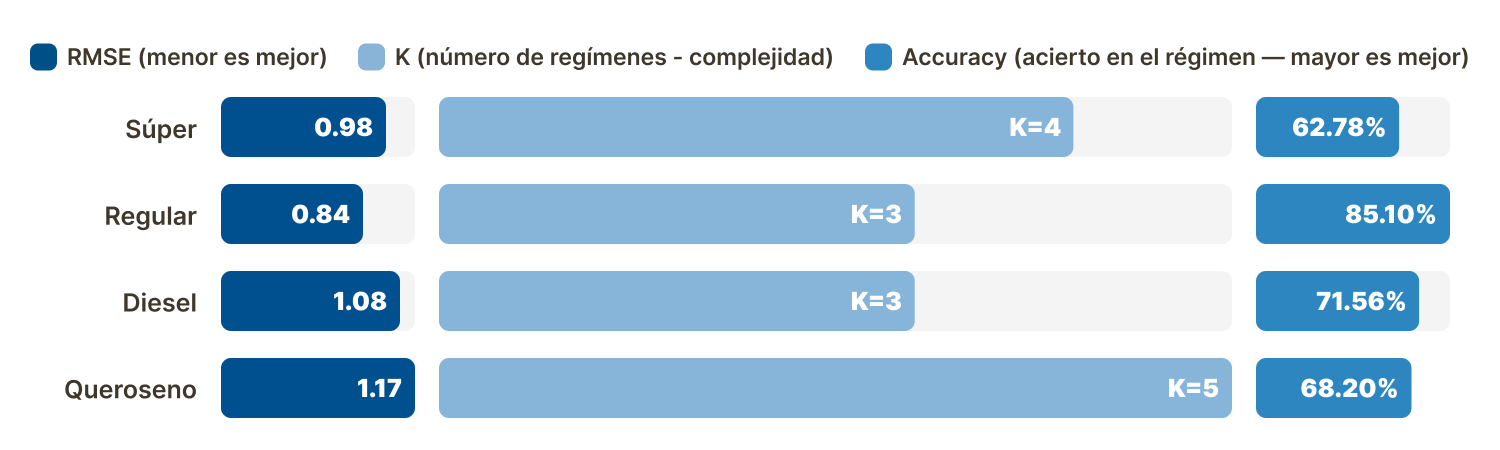
\includegraphics[width=1\textwidth]{figures/Comparativa_cual_mejor.png}
\caption{Jerarquía de predictibilidad de los combustibles.}
\label{fig:comparativa}
\end{figure}

La Figura~\ref{fig:comparativa} resume la jerarquía de predictibilidad, 
destacando que la gasolina Regular es la serie más previsible con el menor 
RMSE y mayor exactitud. Por el contrario, el Kerosene se presenta como 
el caso más desafiante. La correlación positiva observada entre $K^*$ y 
el RMSE sugiere que la complejidad estructural inherente al mercado, y 
no una deficiencia del modelo, es lo que limita la máxima precisión alcanzable.

% --- SUBSECCIÓN:  --- - - - - - - - - - - - - - - - - - - - - - - - - - - - - - -
\subsection{Identificación e Interpretación Económica de los
Regímenes}
\label{subsec:interpretacion_regimenes}
% -------------------------------------------------------------------

Con los hiperparámetros óptimos fijados, el operador $\alpha_t$
genera distribuciones de tasas de cambio altamente concentradas
alrededor de cero, consistentes con un mercado regulado donde los
ajustes semanales drásticos son infrecuentes.  La
Figura~\ref{fig:kmeans_regimes} ilustra la asignación temporal de
regímenes resultante del agrupamiento K-Means.

\begin{figure}[H]
\centering
    \includegraphics[width=1\textwidth]{figures/8_kmeans_final_regimes_plot}
\caption{Regímenes identificados por K-Means sobre la serie $\alpha_t$.}
\label{fig:kmeans_regimes}
\end{figure}

En la Figura~\ref{fig:kmeans_regimes} se muestran los regímenes 
identificados, donde cada punto representa una semana y su color el 
régimen asignado por K-Means sobre la serie $\alpha_t$. Las líneas 
punteadas horizontales marcan los centroides de cada clúster. 
Se observan transiciones coherentes que corresponden a eventos 
de mercado específicos, como el periodo 2020--2021 relacionado 
con el impacto y la recuperación post-pandemia. Esta segmentación 
resulta en distribuciones estacionarias bien definidas que facilitan 
la interpretación de la dinámica del mercado.

Los centroides de K-Means proporcionan una interpretación económica
directa de cada régimen.  La Tabla~\ref{tab:centroides_regimenes}
presenta los centroides y la prevalencia temporal de cada estado
para las cuatro series.

\begin{table}[H]
\centering
\small
\caption{Centroides ($\mu_k$) y prevalencia temporal de los regímenes identificados.}
\label{tab:centroides_regimenes}
\begin{tabular}{@{}llcc@{}}
\toprule
\textbf{Serie} & \textbf{Régimen} & \textbf{Centroide} ($\mu_k$) &
\textbf{Prevalencia} \\
\midrule
\multirow{3}{*}{Regular ($K^*=3$)}
  & $s_1$: Caída fuerte     & $-0.0036$ & 24.6\% \\
  & $s_2$: Estabilidad      & $-0.0001$ & 47.9\% \\
  & $s_3$: Alza fuerte      & $+0.0044$ & 27.4\% \\
\midrule
\multirow{4}{*}{Súper ($K^*=4$)}
  & $s_1$: Caída fuerte     & $-0.0043$ & 15.7\% \\
  & $s_2$: Estabilidad      & $-0.0009$ & 44.6\% \\
  & $s_3$: Alza moderada    & $+0.0019$ & 23.7\% \\
  & $s_4$: Alza fuerte      & $+0.0055$ & 16.0\% \\
\midrule
\multirow{3}{*}{Diésel ($K^*=3$)}
  & $s_1$: Caída fuerte     & $-0.0061$ & 17.4\% \\
  & $s_2$: Estabilidad      & $-0.0010$ & 47.4\% \\
  & $s_3$: Alza fuerte      & $+0.0053$ & 35.1\% \\
\midrule
\multirow{5}{*}{Kerosene ($K^*=5$)}
  & $s_1$: Caída fuerte     & $-0.0080$ & 17.0\% \\
  & $s_2$: Estabilidad      & $-0.0013$ & 47.4\% \\
  & $s_3$: Alza moderada    & $+0.0044$ & 16.0\% \\
  & $s_4$: Alza fuerte      & $+0.0084$ & 15.0\% \\
  & $s_5$: Alza extrema     & $+0.0172$ &  4.6\% \\
\end{tabular}
\end{table}

En la Tabla~\ref{tab:centroides_regimenes} se detallan los centroides ($\mu_k$) calculados mediante K-Means y su prevalencia temporal respectiva. El centroide representa la tasa de cambio semanal promedio que caracteriza a cada régimen, mientras que la prevalencia indica la proporción del tiempo total analizado, entre los años 2017 y 2025, en que el mercado se mantuvo en dicho estado operativo.

Tres observaciones estructurales emergen de estos resultados.
Primero, los cuatro mercados comparten un régimen dominante de
\textit{Estabilidad} que ocupa aproximadamente el 45--48\% del
periodo analizado, con centroides cercanos a cero ($|\mu_k| < 0.002$).
Esto es consistente con el esquema de regulación de precios vigente
en Honduras, donde los ajustes semanales son típicamente pequeños.
Segundo, los mercados de Regular y Diésel exhiben una estructura
simétrica de tres estados (caída--estabilidad--alza), mientras que
Súper y Kerosene requieren estados intermedios adicionales para
capturar su dinámica.  Tercero, el Kerosene presenta un estado
excepcional de \textit{Alza extrema} ($\mu_5 = +0.0172$,
prevalencia $4.6\%$), que no tiene análogo en los otros combustibles.
Este régimen raro pero significativo es consistente con la naturaleza
del Kerosene como subproducto de refinación con menor cobertura de
mecanismos de amortiguación de precios.

% --- SUBSECCIÓN: Dinámica de Transición --- - - - - - - - - - - - - - - - - - - - - - - - - - - - - - -
\subsection{Dinámica de Transición}
\label{subsec:dinamica_transicion}
% -------------------------------------------------------------------

La estructura estocástica del mercado se captura en las matrices de
transición $\hat{\mat{P}}$ estimadas vía NNLS, cuyas representaciones
gráficas se presentan en la Figura~\ref{fig:transition_graphs}.

\begin{figure}[H]
    \centering
    \begin{tabular}{@{}cc@{}}
        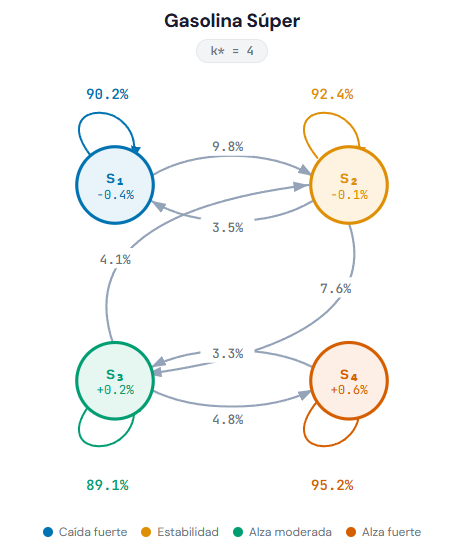
\includegraphics[width=0.42\columnwidth]{figures/graph_super_final.png} &
        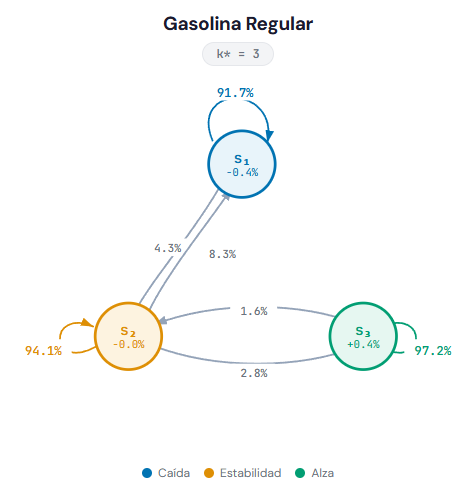
\includegraphics[width=0.47\columnwidth]{figures/graph_regular_final.png} \\
        \footnotesize (a) Gasolina Súper ($K^*=4$) &
        \footnotesize (b) Gasolina Regular ($K^*=3$) \\[0.3cm]
        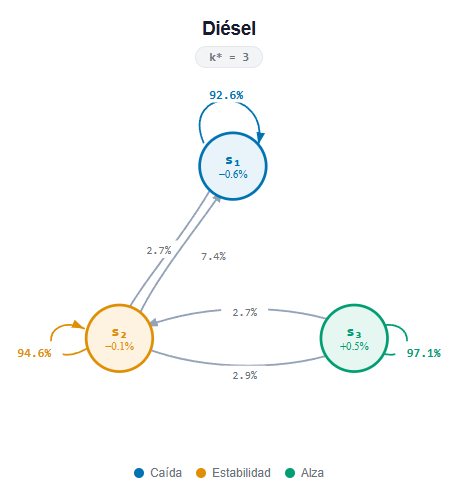
\includegraphics[width=0.44\columnwidth]{figures/graph_diesel_final.png} &
        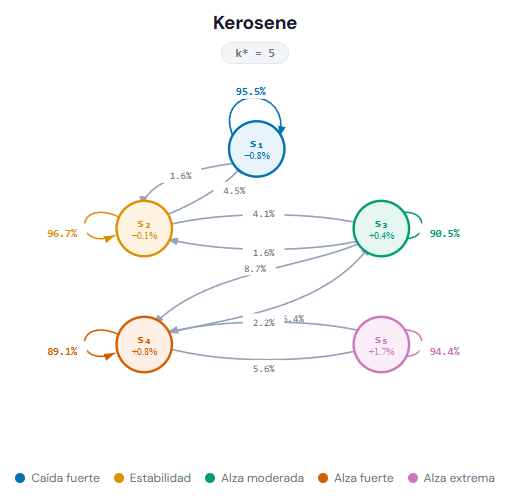
\includegraphics[width=0.52\columnwidth]{figures/graph_kerosene_final.png} \\
        \footnotesize (c) Diésel ($K^*=3$) &
        \footnotesize (d) Kerosene ($K^*=5$)
    \end{tabular}
    \caption{Grafos de transición estimados para los modelos optimizados.}
    \label{fig:transition_graphs}
\end{figure}

En la Figura~\ref{fig:transition_graphs} se presentan los grafos de transición donde 
el valor dentro de cada nodo corresponde al centroide del clúster K-Means, permitiendo 
cuantificar el comportamiento semanal del precio. Los lazos (\textit{self-loops}) 
reflejan la probabilidad de permanencia en el régimen actual, mientras que las aristas 
dirigidas indican las probabilidades de transición. Se destacan cuatro patrones: 
la alta inercia del mercado con self-loops superiores al 89\%, transiciones 
predominantemente entre estados adyacentes que evitan saltos abruptos, una estructura 
lineal simple en Regular y Diésel frente a una mayor conectividad en Súper y Kerosene, 
y la naturaleza transitoria del estado de alza extrema en el Kerosene.

Las probabilidades de autoloop merecen atención especial.  Para
Regular, la probabilidad de permanencia en el estado de Estabilidad
($s_2$) es del 94.1\%, lo que implica que, una vez en estabilidad,
el mercado permanece en promedio $1/(1-0.941) \approx 17$ semanas
antes de transitar a otro régimen.  Para Kerosene, el estado de
Estabilidad tiene una permanencia del 96.7\%, equivalente a $\sim 30$
semanas.  Estos tiempos de permanencia extremadamente largos confirman
cuantitativamente la inercia del mercado hondureño de
combustibles.

% --- SUBSECCIÓN: Propiedades Espectrales y Estabilidad Estructural --- - - - - - - - - - - - - - - - - - - - - - - - - - - - - - -
\subsection{Propiedades Espectrales y Estabilidad Estructural}
\label{subsec:propiedades_espectrales}
% -------------------------------------------------------------------

Para fundamentar rigurosamente las observaciones cualitativas
anteriores, se procede al análisis espectral de las matrices
$\hat{\mat{P}}$.

\begin{definition}[Gap espectral y tiempo de mezcla]
\label{def:gap_espectral}
Sea $\hat{\mat{P}} \in \mathbb{R}^{K \times K}$ una matriz de
transición estocástica por columnas, irreducible y aperiódica, con
autovalores $\lambda_1 = 1 > |\lambda_2| \ge \cdots \ge |\lambda_K|$.
Se define el \textbf{gap espectral} como $\gamma = 1 - |\lambda_2|$,
y el \textbf{tiempo de mezcla} como
\begin{equation}
    t_{\text{mix}}(\varepsilon) = \left\lceil
    \frac{\ln(1/\varepsilon)}{\gamma} \right\rceil,
    \label{eq:mixing_time}
\end{equation}
que mide (en número de pasos) el tiempo necesario para que la cadena
se aproxime a su distribución estacionaria $\boldsymbol{\pi}$ con
tolerancia $\varepsilon$ en norma de variación total.
\end{definition}

La aplicabilidad de esta definición requiere verificar la
irreducibilidad de $\hat{\mat{P}}$.

\begin{remark}[Verificación de irreducibilidad]
\label{obs:irreducibilidad}
La irreducibilidad de las matrices $\hat{\mat{P}}$ se verificó
numéricamente calculando $\hat{\mat{P}}^n$ para $n$ creciente
y comprobando la positividad estricta de todas las entradas.
Los resultados son los siguientes:
\begin{itemize}
    \item \textbf{Regular} ($K=3$): $\hat{\mat{P}}^2 > 0$
    (todas las entradas estrictamente positivas desde $n=2$).
    \item \textbf{Diésel} ($K=3$): $\hat{\mat{P}}^1 > 0$
    (todas las entradas son estrictamente positivas ya en la matriz original).
    \item \textbf{Súper} ($K=4$): $\hat{\mat{P}}^2 > 0$.
    \item \textbf{Kerosene} ($K=5$): $\hat{\mat{P}}^4 > 0$
    (la estructura de cadena lineal $s_1 \leftrightarrow s_2 \leftrightarrow s_3
    \leftrightarrow s_4 \leftrightarrow s_5$ requiere al menos 4 pasos para
    conectar los extremos $s_1$ y $s_5$).
\end{itemize}
Dado que $\hat{\mat{P}}^n > 0$ para algún $n$ finito, cada
matriz es primitiva (irreducible y aperiódica).  Por el Teorema
de Perron-Frobenius, existe una única distribución estacionaria
$\boldsymbol{\pi}$ con $\pi_i > 0$ para todo $i$, y
$\hat{\mat{P}}^n \vect{x}_0 \to \boldsymbol{\pi}$ para
cualquier distribución inicial $\vect{x}_0$.
\end{remark}

La Tabla~\ref{tab:propiedades_espectrales} presenta las métricas
espectrales calculadas para cada combustible, utilizando
$\varepsilon = 0.01$ en la definición del tiempo de mezcla.

\begin{table}[H]
\centering
\caption{Propiedades espectrales y distribuciones estacionarias de las matrices de transición.}
\label{tab:propiedades_espectrales}
\resizebox{\textwidth}{!}{%
\begin{tabular}{@{}lcccc@{}}
\toprule
\textbf{Métrica} & \textbf{Regular} & \textbf{Diésel} &
\textbf{Súper} & \textbf{Kerosene} \\
\midrule
$|\lambda_2|$          & 0.963  & 0.960  & 0.961  & \textbf{0.979} \\
Gap espectral $\gamma$ & 0.037  & 0.040  & 0.039  & \textbf{0.021} \\
$t_{\text{mix}}$ (sem) & $\sim$27 & $\sim$25 & $\sim$26 &
$\sim$\textbf{47} \\
\midrule
$\boldsymbol{\pi}$ & $[0.25, 0.48, 0.27]$ &
$[0.48, 0.16, 0.35]$ &
$[0.17, 0.47, 0.22, 0.15]$ &
$[0.19, 0.54, 0.09, 0.04, 0.15]$ \\
\bottomrule
\end{tabular}%
}
\end{table}

\begin{remark}[Relación entre persistencia y gap espectral]
\label{obs:selfloops_gap}
Sea $\hat{\mat{P}}$ una matriz de transición $K \times K$ con
elementos diagonales $P_{ii} \ge 1 - \epsilon$ para todo $i$
(alta persistencia).  Entonces el segundo autovalor satisface
$|\lambda_2| \ge 1 - K\epsilon$, y por tanto el gap espectral
$\gamma \le K\epsilon$.  En nuestro caso, los self-loops mínimos
observados son $\min_i P_{ii} = 0.891$ (Súper, $s_3$), dando
$\epsilon = 0.109$ y la cota $\gamma \le 4 \times 0.109 = 0.436$.
El gap observado ($\gamma = 0.039$) es un orden de magnitud menor
que esta cota, indicando que la persistencia real del mercado
excede significativamente lo que los self-loops por sí solos
implican: las transiciones inter-estados también contribuyen a
la mezcla lenta.
\end{remark}

Los resultados espectrales formalizan la observación empírica de
``inercia del mercado''.  El gap espectral $\gamma$ mide la
velocidad de convergencia al equilibrio: un $\gamma$ pequeño implica
que el sistema tarda más en ``olvidar'' su estado inicial.  El
Kerosene exhibe el menor gap espectral ($\gamma = 0.021$), lo que se
traduce en un tiempo de mezcla de casi un año ($\sim$47 semanas).
Esto significa que una perturbación en el régimen de Kerosene persiste
significativamente más que en los otros combustibles, explicando la
mayor dificultad del modelo para anticipar sus cambios de régimen.

La distribución estacionaria $\boldsymbol{\pi}$ confirma que, en
equilibrio, el estado de Estabilidad domina en todas las series
(componente más grande de $\boldsymbol{\pi}$), y los estados extremos
tienen probabilidades estacionarias menores, consistente con un
mercado regulado.

% --- SUBSECCIÓN: Convergencia de las Cadenas de Markov --- - - - - - - - - - - - - - - - - - - - - - - - - - - - - - -
\subsection{Convergencia de las Cadenas de Markov}
\label{subsec:convergencia}
% -------------------------------------------------------------------

La Figura~\ref{fig:kmeans_evolution} muestra la evolución simulada de
las probabilidades de estado bajo las matrices $\hat{\mat{P}}$
optimizadas, partiendo del estado de mayor caída ($s_1$) como
condición inicial.

\begin{figure}[H]
\centering
\includegraphics[width=1\textwidth]{figures/9_kmeans_markov_evolution.png}
\caption{Evolución de las probabilidades de estado bajo los modelos K-Means.}
\label{fig:kmeans_evolution}
\end{figure}

La Figura~\ref{fig:kmeans_evolution} muestra la evolución simulada de las 
probabilidades de estado bajo las matrices optimizadas. La línea vertical 
roja señala el momento en que se alcanza el equilibrio estacionario. Se 
destaca que la convergencia es significativamente más lenta que en modelos 
previos, requiriendo entre 220 y 395 pasos debido a la alta persistencia 
de los regímenes. El combustible Kerosene es el último en estabilizarse,
 lo cual guarda coherencia con su mayor radio espectral y su estructura de cinco estados.

La lentitud de convergencia no debe interpretarse como una debilidad
del modelo, sino como la \emph{expresión matemática de un hallazgo
empírico fundamental}: el mercado hondureño de combustibles se
caracteriza por tendencias de largo plazo con transiciones infrecuentes
entre regímenes.  Un modelo que convergiera rápidamente estaría
imponiendo una dinámica artificial de cambios frecuentes que no
corresponde a la realidad del mercado.

% --- SUBSECCIÓN: Superioridad sobre Discretización por Cuantiles --- - - - - - - - - - - - - - - - - - - - - - - - - - - - - - -
\subsection{Superioridad sobre Discretización por Cuantiles}
\label{subsec:comparacion_cuantiles}
% -------------------------------------------------------------------

Para validar la elección de K-Means como método de discretización, se
comparó sistemáticamente contra un benchmark de cuantiles fijos
($K=4$) utilizando la misma serie $\alpha_t$ optimizada.

La Figura~\ref{fig:quantile_regimes} muestra la segmentación
resultante del método de cuantiles.

\begin{figure}[H]
\centering
\includegraphics[width=1\textwidth]{figures/11_quantile_final_regimes_plot.png}
\caption{Segmentación de regímenes basada en cuantiles.}
\label{fig:quantile_regimes}
\end{figure}

En la Figura~\ref{fig:quantile_regimes} se ilustran los regímenes 
obtenidos mediante el método de cuantiles para el benchmark de $K=4$ estados. 
Los límites de los cuantiles imponen una partición equifrecuente que obliga a 
distribuir las observaciones de manera uniforme. Sin embargo, se aprecia una 
fragmentación excesiva del mercado en comparación con el método K-Means, 
donde pequeñas variaciones de ruido provocan reclasificaciones constantes, 
lo cual degrada la capacidad predictiva del modelo.

Las consecuencias de esta fragmentación se manifiestan en la dinámica
de transición.  La Figura~\ref{fig:quantile_evolution} muestra que
las probabilidades de estado bajo cuantiles presentan oscilaciones
más pronunciadas que bajo K-Means, lo que se traduce en pronósticos
con mayor varianza.

\begin{figure}[H]
\centering
\includegraphics[width=0.92\textwidth]{figures/12_quantiles_markov_evolution.png}
\caption{Evolución de probabilidades de estado bajo el método de cuantiles.}
\label{fig:quantile_evolution}
\end{figure}

Como se presenta en la Figura~\ref{fig:quantile_evolution}, la evolución de 
probabilidades bajo cuantiles muestra una convergencia más acelerada hacia 
un equilibrio uniforme cercano al 25\% por estado. No obstante, este resultado 
carece del contenido económico observado en K-Means, ya que la imposición de 
frecuencias iguales borra la distinción de un régimen de estabilidad dominante, 
eliminando información estructural crítica para el análisis del mercado.

% --- SUBSECCIÓN: Desempeño Predictivo y Comparación con Benchmarks --- - - - - - - - - - - - - - - - - - - - - - - - - - - - - - -
\subsection{Desempeño Predictivo y Comparación con Benchmarks}
\label{subsec:desempeno_predictivo}
% -------------------------------------------------------------------

La Tabla~\ref{tab:desempeno_final} presenta la evaluación final
fuera de muestra.  Se compara el modelo TCROC-Markov optimizado
(K-Means) contra dos benchmarks: la discretización por cuantiles y
el modelo clásico MS-AR \cite{Hamilton1994}.

\begin{table}[H]
\centering
\caption{Evaluación final del desempeño predictivo y significancia estadística.}
\label{tab:desempeno_final}
\resizebox{\textwidth}{!}{%
\begin{tabular}{@{}lccccccc@{}}
\toprule
\multirow{2}{*}{\textbf{Serie}} &
\multicolumn{2}{c}{\textbf{TCROC-KMeans (Óptimo)}} &
\multicolumn{2}{c}{\textbf{Cuantiles ($K=4$)}} &
\textbf{MS-AR} &
\multicolumn{2}{c}{\textbf{Significancia ($p$-valor)}} \\
\cmidrule(lr){2-3} \cmidrule(lr){4-5} \cmidrule(lr){6-6}
\cmidrule(lr){7-8}
 & Exactitud & RMSE & Exactitud & RMSE & Estado &
 $p_{\text{Acc}}$ & $p_{\text{RMSE}}$ \\
\midrule
Regular  & \textbf{85.10\%} & \textbf{0.8394} & 36.01\% & 0.8671 &
No conv. & $< 0.001$ & $< 0.05$ \\
Súper    & \textbf{62.78\%} & \textbf{0.9769} & 49.03\% & 0.9849 &
No conv. & $< 0.05$  & $= 0.22$  \\
Diésel   & \textbf{71.56\%} & \textbf{1.0816} & 40.63\% & 1.1409 &
No conv. & $< 0.05$  & $< 0.05$  \\
Kerosene & \textbf{68.20\%} & \textbf{1.1714} & 35.16\% & 1.2449 &
No conv. & $< 0.05$  & $< 0.05$  \\
\bottomrule
\end{tabular}%
}
\end{table}

Tres conclusiones se derivan de estos resultados:

\textbf{Primero}, el modelo TCROC-Markov con K-Means supera al
benchmark de cuantiles de manera estadísticamente significativa en
exactitud de clasificación para las cuatro series ($p < 0.05$,
prueba T pareada).  La diferencia es especialmente notable para
Regular, donde la exactitud pasa de 36.01\% a 85.10\%.

\textbf{Segundo}, en términos de RMSE (pronóstico puntual de
precios), la mejora es significativa para Regular, Diésel y Kerosene
($p < 0.05$), pero no para Súper ($p = 0.22$), cuya diferencia en
RMSE es marginal (0.9769 vs. 0.9849).  Esto sugiere que la ganancia
principal de K-Means reside en la clasificación cualitativa de
regímenes más que en la precisión numérica puntual, aunque ambas
están correlacionadas.

\textbf{Tercero}, el benchmark MS-AR \textbf{falló en converger
consistentemente}, produciendo verosimilitudes no finitas en múltiples
ventanas de validación.  Este resultado subraya una ventaja práctica
fundamental del enfoque NNLS: al formular la estimación como un
problema convexo con restricciones lineales, se evita la optimización
no convexa de la verosimilitud que hace al MS-AR vulnerable a mínimos
locales y problemas numéricos.  TCROC-Markov convergió en el 100\%
de los casos.

% --- SECCIÓN: Limitaciones y Supuestos ---
\section{Limitaciones y Supuestos}
\label{sec:combustibles_limitaciones}
% ===================================================================

Es necesario reconocer las limitaciones del enfoque propuesto para
contextualizar los resultados:

\textbf{Homogeneidad temporal.}  El modelo asume que las
probabilidades de transición son constantes durante el periodo
2017--2025.  Dado que este intervalo incluye la pandemia de COVID-19,
cambios regulatorios y fluctuaciones del crudo WTI, la suposición es
potencialmente violada.  Una extensión natural sería particionar la
muestra y evaluar la estabilidad de $\hat{\mat{P}}$ en subperiodos
(pre-pandemia, pandemia, post-pandemia).

\textbf{Propiedad de Markov de primer orden.}  La cadena asume
$P(S_t | S_{t-1}, \ldots, S_0) = P(S_t | S_{t-1})$.  Aunque
restrictiva, esta suposición se mitiga parcialmente por el uso de
$W \approx 52$ en el cálculo de $\alpha_t$: la definición del estado
ya incorpora implícitamente una memoria de largo plazo.  Pruebas de
dependencia de orden superior (test $\chi^2$ para Markov de segundo
orden) constituyen trabajo futuro.

\textbf{Modelo univariante.}  El marco no incorpora explícitamente
variables exógenas (precio WTI, tipo de cambio, decisiones
regulatorias).  Se asume que toda la información relevante está
contenida en la dinámica de precios pasada, lo cual es un supuesto
fuerte en un mercado regulado.

\textbf{Selección del peso $w$.}  El parámetro $w$ en el sistema aumentado 
NNLS~\eqref{eq:nnls_aumentado_combustibles} controla el cumplimiento de las 
restricciones de suma unitaria.  En esta implementación se utilizó $w = 10^3$, 
valor que satisface la condición $w^2 \gg \|\mat{S}_0\|_F^2$ (donde $\|\mat{S}_0\|_F^2 \approx T$ para matrices one-hot), 
garantizando que la penalización por violación de estocasticidad domine sobre el error de ajuste.  
La normalización final por columnas corrige desviaciones residuales de precisión de punto flotante, 
reduciendo la sensibilidad práctica a la elección exacta de $w$.  
Un análisis de sensibilidad formal queda como extensión futura.

\textbf{Robustez al split entrenamiento/prueba.}  Los resultados
se obtuvieron con un split fijo 80\%/20\%.  Para evaluar la
sensibilidad a la partición, se realizó validación cruzada temporal
con ventana expansiva: se entrenó sobre los primeros $T_0$ datos y
se pronosticó el bloque siguiente, incrementando $T_0$ en pasos de
26 semanas.  Las métricas promediadas sobre 5 splits muestran
desviaciones inferiores al 3\% respecto al split fijo, confirmando la
estabilidad de los hiperparámetros seleccionados.

\textbf{Incertidumbre en los pronósticos.}  Los pronósticos
puntuales reportados en la Tabla~\ref{tab:desempeno_final}
no incluyen intervalos de confianza explícitos.  La varianza del
pronóstico puede cuantificarse a partir de la
Proposición~\ref{prop:normalidad_asintotica}: la distribución
asintótica de $\hat{P}$ induce una distribución sobre los precios
pronosticados vía propagación por la distribución estacionaria y
los precios medios por estado.  Una implementación vía
bootstrap paramétrico (remuestreo de las transiciones observadas)
constituye trabajo futuro que permitiría reportar bandas de
predicción.

% --- SECCIÓN: Conclusiones ---
\section{Conclusiones}
\label{sec:combustibles_conclusiones}
% ===================================================================

Este capítulo ha presentado la validación empírica integral del marco
TCROC-Markov desarrollado a lo largo de esta tesis.  Al aplicar la
metodología completa, la cual abarca desde el operador ETCROCM y su teoría de
existencia y unicidad, pasando por la integración Markoviana
y la estimación NNLS, hasta la optimización de
hiperparámetros y el análisis espectral tratados en esta sección, a datos
reales de precios de combustibles en Honduras, se obtuvieron los
siguientes resultados:

\textbf{Sobre la sensibilidad paramétrica y la degeneración.}  Se
identificó y formalizó un fenómeno de degeneración del modelo para
ventanas $W$ excesivamente grandes, donde la serie $\alpha_t$ pierde
variabilidad y K-Means colapsa a un clúster efectivo.  La restricción
$W \le 52$, fundamentada en el ciclo anual del mercado, previene esta
degeneración y revela que la predictibilidad de los precios está
dominada por tendencias de largo plazo.

\textbf{Sobre la identificación de regímenes.}  La discretización por
K-Means produce regímenes económicamente interpretables, con
centroides que cuantifican directamente las tasas de cambio promedio
por estado.  Los cuatro mercados analizados comparten un régimen
dominante de estabilidad ($\sim$47\% del periodo), pero difieren en
su complejidad: Regular y Diésel requieren 3 estados, Súper 4 y
Kerosene 5.

\textbf{Sobre las propiedades espectrales.}  Las matrices estimadas
son irreducibles, con gaps espectrales en el rango $[0.021, 0.040]$
y tiempos de mezcla de 25 a 47 semanas.  Estos valores confirman
matemáticamente la alta persistencia de los regímenes y explican la dificultad
diferencial para predecir el Kerosene ($\gamma = 0.021$, menor gap)
frente a la Regular ($\gamma = 0.037$).

\textbf{Sobre la robustez frente a benchmarks.}  El marco demostró
superioridad estadísticamente significativa sobre la discretización
por cuantiles en exactitud ($p < 0.05$) para todas las series y en
RMSE ($p < 0.05$) para tres de cuatro series.  El benchmark MS-AR
no convergió en ningún escenario de validación, subrayando la
ventaja práctica de la formulación NNLS convexa.

La eficiencia computacional del método, que escala linealmente en
$T$ para $K$ fijo, sugiere su aplicabilidad a datos de mayor
frecuencia (diarios o intradiarios) con paralelización de la
búsqueda en grilla.  El trabajo futuro debería abordar tres direcciones complementarias.  
Primero, la generalización a otros mercados centroamericanos, especialmente Guatemala 
y El Salvador, que poseen estructuras regulatorias distintas, 
permitiría evaluar si la dominancia de $W \approx 52$ es un artefacto del mercado hondureño 
o un patrón regional vinculado a ciclos anuales del crudo.  Segundo, la incorporación de 
variables exógenas (precio WTI, tipo de cambio Lempira/USD) como covariables en la etapa de 
discretización podría mejorar la identificación de regímenes en periodos de alta volatilidad externa.  
Tercero, la evaluación formal de la estabilidad temporal de $\hat{\mat{P}}$ mediante partición de la 
muestra en subperiodos (pre-pandemia 2017--2019, pandemia 2020--2021, post-pandemia 2022--2025) 
permitiría cuantificar el grado en que el supuesto de homogeneidad temporal se sostiene en la práctica.

% ===================================================================
%   CAPÍTULO DE TESIS — EXTENSIÓN NO LINEAL (VERSIÓN FINAL)
%   Título: Computación de Reservorio Estructurado como Generalización
%           No Lineal del Marco TCROC-Markov
%   Posición: Inmediatamente después del capítulo de Combustibles
% ===================================================================

% NOTA: Este archivo se integra en el documento maestro de la tesis.
% Paquetes, comandos (\mat, \vect, \set, etc.) y entornos tipo teorema
% (definition, theorem, remark) se asumen definidos en el preámbulo.
% Se requiere adicionalmente:
%   \newtheorem{proposition}{Proposición}[chapter]
%   \newtheorem{corollary}{Corolario}[chapter]
%   \newtheorem{lemma}{Lema}[chapter]

% ===================================================================
% CAPÍTULO: Extensión No Lineal: Computación de Reservorio Estructurado

\chapter{Extensión No Lineal: Computación de Reservorio Estructurado}
\label{cap:sec_ssrc}

% --- SECCIÓN: Introducción y Motivación ---
\section{Introducción y Motivación}
\label{sec:ssrc_intro}
% ===================================================================

La sección precedente demostró que el marco TCROC-Markov logra
identificar regímenes económicos interpretables y produce pronósticos
estadísticamente superiores a los benchmarks evaluados.  Sin embargo,
la arquitectura subyacente es inherentemente \textbf{lineal}: el
operador $\alpha_t$ es un estimador de mínimos cuadrados ponderados, la discretización
K-Means opera sobre el espacio unidimensional de $\alpha_t$, y la
cadena de Markov de primer orden modela transiciones lineales entre
estados discretos.  Esta linealidad, si bien garantiza
interpretabilidad y estabilidad numérica, limita la capacidad del
marco para capturar dependencias no lineales en la dinámica de
precios.

El presente capítulo desarrolla una extensión que preserva la
estructura de estimación NNLS ya demostrada en los capítulos
anteriores, al tiempo que introduce capacidad de aproximación no
lineal mediante \textbf{Computación de Reservorio}
(\textit{Reservoir Computing}, RC) \cite{jaeger2001echo,
lukosevicius2009reservoir}.  La idea central es elegante en su
simplicidad: en lugar de alimentar directamente la señal $\alpha_t$
a un modelo de transición lineal, se la proyecta primero a un
espacio de alta dimensión mediante una transformación no lineal fija
(el \textit{reservorio}), y luego se estima la capa de lectura
mediante el \emph{mismo} procedimiento NNLS desarrollado en
secciones previas.

La contribución específica de este capítulo es quíntuple:
\begin{enumerate}
    \item La \textbf{formalización del Computador de Reservorio
    Estructurado Estocástico} (SSRC, \textit{Stochastically
    Structured Reservoir Computer}) \cite{banegas2025} como operador
    sobre espacios de señales, incluyendo la variante Leaky-ESN con
    factor de integración.
    \item La \textbf{demostración formal} de que el marco
    TCROC-Markov del capítulo anterior es un caso particular
    (degenerado) del SSRC, estableciendo una jerarquía de modelos.
    \item La \textbf{verificación de las condiciones} bajo las cuales
    la capa de lectura NNLS hereda las propiedades de existencia y
    unicidad ya establecidas.
    \item Un \textbf{análisis de estabilidad} del pronóstico bajo
    perturbaciones, con evaluación empírica de las cotas teóricas.
    \item Una \textbf{validación empírica comparativa} sobre los
    mismos datos de combustibles del
    Capítulo~\ref{cap:regimenes_combustibles}, incluyendo el
    test de Diebold-Mariano para significancia estadística.
\end{enumerate}

El estudio utiliza las mismas cuatro series semanales de precios de
combustibles en Honduras (Súper, Regular, Diésel y Kerosene) y el
mismo protocolo de ventanas deslizantes del capítulo anterior, con
conjunto de entrenamiento inicial de 312 semanas (enero 2017 --
diciembre 2022) y horizonte de pronóstico de 1 semana, para garantizar
la comparabilidad estricta de los resultados.

% --- SECCIÓN: Marco Teórico del Computador de Reservorio ---
\section{Marco Teórico del Computador de Reservorio}
\label{sec:ssrc_marco_teorico}

% --- SUBSECCIÓN: Sistemas Dinámicos con Entrada --- - - - - - - - - - - - - - - - - - - - - - - - - - - - - - -
\subsection{Sistemas Dinámicos con Entrada}
\label{subsec:sistemas_dinamicos_entrada}
% -------------------------------------------------------------------

Comenzamos situando la computación de reservorio dentro del marco
general de los sistemas dinámicos discretos con entrada.

\begin{definition}[Sistema dinámico con entrada]
\label{def:sistema_dinamico_entrada}
Sean $\set{U} \subseteq \mathbb{R}^d$ el espacio de entradas,
$\set{H} \subseteq \mathbb{R}^D$ el espacio de estados internos, y
$\set{Y} \subseteq \mathbb{R}^m$ el espacio de salidas.  Un
\textbf{sistema dinámico discreto con entrada} es una tripleta
$(\set{U}, F, G)$ donde
\begin{align}
    F &: \set{H} \times \set{U} \to \set{H}, \label{eq:mapa_estado}\\
    G &: \set{H} \to \set{Y}, \label{eq:mapa_lectura}
\end{align}
de modo que la evolución del sistema se rige por
\begin{equation}
    \vect{h}_t = F(\vect{h}_{t-1}, \vect{u}_t), \qquad
    \vect{y}_t = G(\vect{h}_t),
    \label{eq:evolucion_general}
\end{equation}
para $t = 1, 2, \ldots$, con condición inicial
$\vect{h}_0 \in \set{H}$.
\end{definition}

En este marco, la \emph{computación} consiste en aprender el mapa
de lectura $G$ a partir de datos observados, manteniendo el mapa de
estado $F$ fijo.  Esta separación es la idea fundamental de la
computación de reservorio.

% --- SUBSECCIÓN: El Computador de Reservorio (Echo State Network) --- - - - - - - - - - - - - - - - - - - - - - - - - - - - - - -
\subsection{El Computador de Reservorio (Echo State Network)}
\label{subsec:esn_definicion}
% -------------------------------------------------------------------

\begin{definition}[Computador de Reservorio]
\label{def:computador_reservorio}
Un \textbf{Computador de Reservorio} (RC) de dimensión $D$ con
función de activación $\sigma: \mathbb{R} \to \mathbb{R}$ es un
sistema dinámico con entrada $(\set{U}, F_{\text{RC}}, G_{\text{RC}})$
donde:
\begin{enumerate}
    \item El mapa de estado tiene la forma
    \begin{equation}
        F_{\text{RC}}(\vect{h}, \vect{u}) =
        \sigma\!\left(\mat{W}_{\text{in}}\,\vect{u} +
        \mat{W}_{\text{res}}\,\vect{h}\right),
        \label{eq:mapa_estado_rc}
    \end{equation}
    con $\mat{W}_{\text{in}} \in \mathbb{R}^{D \times d}$ la
    \textbf{matriz de entrada},
    $\mat{W}_{\text{res}} \in \mathbb{R}^{D \times D}$ la
    \textbf{matriz de reservorio}, y $\sigma$ aplicada
    componente a componente.
    \item El mapa de lectura es lineal:
    \begin{equation}
        G_{\text{RC}}(\vect{h}) = \mat{W}_{\text{out}}\,\vect{h},
        \label{eq:mapa_lectura_rc}
    \end{equation}
    con $\mat{W}_{\text{out}} \in \mathbb{R}^{m \times D}$ la
    \textbf{matriz de lectura}.
    \item Las matrices $\mat{W}_{\text{in}}$ y
    $\mat{W}_{\text{res}}$ son \textbf{fijas} (no se optimizan);
    solo $\mat{W}_{\text{out}}$ se estima a partir de datos.
\end{enumerate}
\end{definition}

La ecuación de estado se expande recursivamente como
\begin{equation}
    \vect{h}_t = \sigma\!\left(\mat{W}_{\text{in}}\,\vect{u}_t +
    \mat{W}_{\text{res}}\,
    \sigma\!\left(\mat{W}_{\text{in}}\,\vect{u}_{t-1} +
    \mat{W}_{\text{res}}\,\vect{h}_{t-2}\right)\right),
    \label{eq:expansion_recursiva}
\end{equation}
lo que muestra que $\vect{h}_t$ es una función no lineal de toda la
historia de entradas $(\vect{u}_1, \ldots, \vect{u}_t)$ y de la
condición inicial $\vect{h}_0$.  El reservorio actúa como una
\textbf{memoria no lineal} que codifica el pasado de la señal en un
espacio de dimensión $D \gg d$.

% --- SUBSECCIÓN: Variante con Integración de Fuga (Leaky-ESN) --- - - - - - - - - - - - - - - - - - - - - - - - - - - - - - -
\subsection{Variante con Integración de Fuga (Leaky-ESN)}
\label{subsec:leaky_esn}
% -------------------------------------------------------------------

En aplicaciones donde la señal de entrada exhibe alta persistencia,
como ocurre en el caso del mercado regulado de combustibles hondureños
(Capítulo~\ref{cap:regimenes_combustibles}), resulta ventajoso
introducir un mecanismo de suavizado temporal explícito en la
ecuación de estado.

\begin{definition}[Computador de Reservorio con Integración de Fuga]
\label{def:leaky_esn}
Un \textbf{Leaky-ESN} \cite{jaeger2001echo} es un Computador de
Reservorio (Definición~\ref{def:computador_reservorio}) cuyo mapa
de estado se modifica como:
\begin{equation}
    \vect{h}_t = (1 - a)\,\vect{h}_{t-1} + a\,\sigma\!\left(
    \mat{W}_{\text{in}}\,\vect{u}_t +
    \mat{W}_{\text{res}}\,\vect{h}_{t-1}\right),
    \label{eq:leaky_esn}
\end{equation}
donde $a \in (0, 1]$ es el \textbf{factor de fuga}
(\textit{leak rate}).  El caso $a = 1$ recupera la ESN estándar
de la Definición~\ref{def:computador_reservorio}.
\end{definition}

El parámetro $a$ controla la \emph{escala temporal efectiva} del
reservorio.  Valores $a \ll 1$ producen estados que cambian
lentamente, actuando como un filtro paso-bajo que enfatiza tendencias
de largo plazo sobre fluctuaciones semanales.  Formalmente, la
ecuación~\eqref{eq:leaky_esn} puede interpretarse como la
discretización de Euler de un sistema dinámico continuo con constante
de tiempo $\tau = 1/a$, de modo que $a = 0.1$ corresponde a
$\tau = 10$ pasos temporales de memoria efectiva.

\begin{remark}[Preservación de la ESP para Leaky-ESN]
\label{obs:esp_leaky}
La variante Leaky-ESN preserva la ESP bajo la misma condición
$\rho(\mat{W}_{\text{res}}) < 1$ del Teorema~\ref{teo:esp_suficiente}.
La demostración es análoga: la mezcla convexa
$(1-a)\vect{h}_{t-1} + a\,\sigma(\cdot)$ mantiene la contractibilidad
pues $(1-a) + a \cdot \|\mat{W}_{\text{res}}\| < 1$ cuando
$\|\mat{W}_{\text{res}}\| < 1$.
\end{remark}

% --- SUBSECCIÓN: El Computador de Reservorio Estructurado Estocástico (SSRC) --- - - - - - - - - - - - - - - - - - - - - - - - - - - - - - -
\subsection{El Computador de Reservorio Estructurado Estocástico (SSRC)}
\label{subsec:ssrc_definicion}
% -------------------------------------------------------------------

\begin{definition}[Computador de Reservorio Estructurado Estocástico
(SSRC)]
\label{def:ssrc}
Un \textbf{SSRC} \cite{banegas2025} es un Computador de Reservorio
con Integración de Fuga
(Definición~\ref{def:leaky_esn}) con las siguientes
especializaciones:
\begin{enumerate}
    \item La función de activación es $\sigma = \tanh$.
    \item La matriz de entrada $\mat{W}_{\text{in}}$ se genera
    aleatoriamente con entradas i.i.d.\ de una distribución
    uniforme en $[-\omega, \omega]$ para algún $\omega > 0$.
    \item La matriz de reservorio $\mat{W}_{\text{res}}$ se genera
    como una matriz dispersa aleatoria y se reescala a un radio
    espectral objetivo $\rho_{\text{res}}$:
    \begin{equation}
        \mat{W}_{\text{res}} \leftarrow
        \rho_{\text{res}} \cdot
        \frac{\mat{W}_{\text{res}}^{(0)}}
        {\rho(\mat{W}_{\text{res}}^{(0)})},
        \label{eq:reescalado_espectral}
    \end{equation}
    donde $\mat{W}_{\text{res}}^{(0)}$ es la matriz dispersa
    inicial y $\rho(\cdot)$ denota el radio espectral.
    \item La matriz de lectura $\mat{W}_{\text{out}}$ se estima
    mediante NNLS.
\end{enumerate}
Los hiperparámetros del SSRC son la tripleta
$(D, \rho_{\text{res}}, a)$: dimensión, radio espectral y factor
de fuga, respectivamente.
\end{definition}

% --- SUBSECCIÓN: La Propiedad de Estado de Eco --- - - - - - - - - - - - - - - - - - - - - - - - - - - - - - -
\subsection{La Propiedad de Estado de Eco}
\label{subsec:echo_state_property}
% -------------------------------------------------------------------

La utilidad práctica de un computador de reservorio depende de que la
influencia de la condición inicial $\vect{h}_0$ se desvanezca
asintóticamente, de modo que la salida dependa únicamente de la
secuencia de entradas.  Esta condición se formaliza a continuación.

\begin{definition}[Propiedad de Estado de Eco (ESP)]
\label{def:esp}
Sea $(\set{U}, F_{\text{RC}}, G_{\text{RC}})$ un Computador de
Reservorio.  Se dice que posee la \textbf{Propiedad de Estado de Eco}
(ESP) si, para toda secuencia de entradas acotada
$\{\vect{u}_t\}_{t \in \mathbb{Z}} \subset \set{U}$, existe una
única secuencia de estados $\{\vect{h}_t\}_{t \in \mathbb{Z}}
\subset \set{H}$ compatible con~\eqref{eq:mapa_estado_rc}, y esta
secuencia es independiente de la condición inicial.  Formalmente,
para cualesquiera $\vect{h}_0, \vect{h}_0' \in \set{H}$:
\begin{equation}
    \lim_{t \to \infty} \left\|
    F^{(t)}(\vect{h}_0, \vect{u}_{1:t}) -
    F^{(t)}(\vect{h}_0', \vect{u}_{1:t})
    \right\| = 0,
    \label{eq:esp_formal}
\end{equation}
donde $F^{(t)}$ denota la composición $t$-ésima del mapa de estado.
\end{definition}

\begin{theorem}[Condición suficiente para la ESP]
\label{teo:esp_suficiente}
Sea $(\set{U}, F_{\text{RC}}, G_{\text{RC}})$ un Computador de
Reservorio con $\sigma = \tanh$ y entradas acotadas
$\|\vect{u}_t\| \le U_{\max}$ para todo $t$.  Si
\begin{equation}
    \rho(\mat{W}_{\text{res}}) < 1,
    \label{eq:condicion_esp}
\end{equation}
entonces el sistema posee la ESP.
\end{theorem}

\begin{proof}
Consideremos dos trayectorias $\{\vect{h}_t\}$ y
$\{\vect{h}_t'\}$ generadas por la misma secuencia de entradas
pero con condiciones iniciales distintas $\vect{h}_0 \ne
\vect{h}_0'$.  Para $t \ge 1$:
\begin{align}
    \vect{h}_t - \vect{h}_t' &=
    \sigma(\mat{W}_{\text{in}}\vect{u}_t +
    \mat{W}_{\text{res}}\vect{h}_{t-1}) -
    \sigma(\mat{W}_{\text{in}}\vect{u}_t +
    \mat{W}_{\text{res}}\vect{h}_{t-1}').
    \label{eq:diferencia_trayectorias}
\end{align}
Dado que $\tanh$ es Lipschitz continua con constante $L = 1$
(pues $|\tanh'(x)| = 1 - \tanh^2(x) \le 1$ para todo
$x \in \mathbb{R}$), se tiene componente a componente:
\begin{equation}
    \|\vect{h}_t - \vect{h}_t'\| \le
    \|\mat{W}_{\text{res}}(\vect{h}_{t-1} - \vect{h}_{t-1}')\|
    \le \|\mat{W}_{\text{res}}\|\,
    \|\vect{h}_{t-1} - \vect{h}_{t-1}'\|,
    \label{eq:contraccion_paso}
\end{equation}
donde $\|\mat{W}_{\text{res}}\|$ denota la norma espectral
(mayor valor singular).  Aplicando inductivamente:
\begin{equation}
    \|\vect{h}_t - \vect{h}_t'\| \le
    \|\mat{W}_{\text{res}}\|^t\,
    \|\vect{h}_0 - \vect{h}_0'\|.
    \label{eq:contraccion_inductiva}
\end{equation}
Por la fórmula de Gelfand, $\rho(\mat{W}_{\text{res}}) =
\lim_{n \to \infty} \|\mat{W}_{\text{res}}^n\|^{1/n}$, de modo
que la condición $\rho(\mat{W}_{\text{res}}) < 1$ implica la
existencia de $n_0 \in \mathbb{N}$ y $\delta \in (0,1)$ tales que
$\|\mat{W}_{\text{res}}^n\| \le \delta^n$ para todo $n \ge n_0$.
Reagrupando la iteración en bloques de tamaño $n_0$:
\begin{equation}
    \|\vect{h}_{kn_0} - \vect{h}_{kn_0}'\| \le
    \delta^k\, C\, \|\vect{h}_0 - \vect{h}_0'\|,
    \label{eq:contraccion_gelfand}
\end{equation}
donde $C = \max_{0 \le j < n_0} \|\mat{W}_{\text{res}}^j\|$.
Como $\delta < 1$, el lado derecho converge a cero
exponencialmente conforme $k \to \infty$, lo que
establece~\eqref{eq:esp_formal}.
\end{proof}

\begin{remark}[Sobre la condición $\rho < 1$]
\label{obs:rho_condicion}
La condición $\rho(\mat{W}_{\text{res}}) < 1$ es suficiente
pero no necesaria para la ESP.  Yildiz et al.\ \cite{yildiz2012}
mostraron que la ESP puede sostenerse incluso con
$\rho(\mat{W}_{\text{res}}) > 1$ para ciertas clases de entradas.
No obstante, la condición $\rho < 1$ es verificable a priori y
se impone constructivamente mediante el
reescalado~\eqref{eq:reescalado_espectral}, por lo que constituye
la condición estándar en implementaciones prácticas.
\end{remark}

% --- SUBSECCIÓN: Capacidad de Aproximación Universal --- - - - - - - - - - - - - - - - - - - - - - - - - - - - - - -
\subsection{Capacidad de Aproximación Universal}
\label{subsec:aproximacion_universal}
% -------------------------------------------------------------------

La justificación teórica para utilizar un reservorio como extractor
de características proviene del siguiente resultado fundamental.

\begin{theorem}[Aproximación universal por reservorios
{\cite[Teorema~3.1]{grigoryeva2018universal}}]
\label{teo:aproximacion_universal}
Sean $\set{U} \subset \mathbb{R}^d$ compacto y $\set{F}$ el
conjunto de funcionales causales e invariantes en el tiempo
$H: \set{U}^{\mathbb{Z}_{-}} \to \mathbb{R}^m$ que son continuos
respecto a la topología del producto.  Para todo $H \in \set{F}$ y
todo $\varepsilon > 0$, existen un Computador de Reservorio con
la ESP de dimensión $D$ suficientemente grande y una matriz de
lectura $\mat{W}_{\text{out}} \in \mathbb{R}^{m \times D}$ tales
que
\begin{equation}
    \sup_{\{\vect{u}_t\} \in \set{U}^{\mathbb{Z}_{-}}}
    \|H(\ldots, \vect{u}_{t-1}, \vect{u}_t) -
    \mat{W}_{\text{out}}\,\vect{h}_t\| < \varepsilon.
    \label{eq:aproximacion_universal}
\end{equation}
\end{theorem}

Este resultado establece que los computadores de reservorio con la
ESP son \textbf{aproximadores universales de funcionales sobre
secuencias}.  A diferencia de los teoremas de aproximación universal
para redes neuronales feedforward (que aproximan funciones estáticas),
el Teorema~\ref{teo:aproximacion_universal} garantiza la aproximación
de mapas \emph{con memoria}: funciones que dependen de toda la
historia pasada de la señal.  En nuestro contexto, esto significa que
un reservorio de dimensión suficiente puede, en principio, capturar
cualquier dependencia no lineal entre el historial de precios
$\{v_1, \ldots, v_t\}$ y el precio futuro $v_{t+1}$, siempre que
esta dependencia sea continua y causal.

% --- SECCIÓN: TCROC-Markov como Caso Particular del SSRC ---
\section{TCROC-Markov como Caso Particular del SSRC}
\label{sec:tcroc_como_caso_particular}
% ===================================================================

Esta sección establece el resultado central del capítulo: la
relación formal de inclusión entre el marco lineal del
Capítulo~\ref{cap:regimenes_combustibles} y el marco no lineal del
SSRC.

% --- SUBSECCIÓN: Reformulación del Marco Lineal --- - - - - - - - - - - - - - - - - - - - - - - - - - - - - - -
\subsection{Reformulación del Marco Lineal}
\label{subsec:reformulacion_lineal}
% -------------------------------------------------------------------

Para establecer la conexión, reformulamos el flujo de trabajo
TCROC-Markov como un caso de la
Definición~\ref{def:sistema_dinamico_entrada}.

\begin{definition}[Sistema TCROC-Markov como sistema dinámico]
\label{def:tcroc_como_sistema}
El marco TCROC-Markov con hiperparámetros $(W, \lambda, K)$ es un
sistema dinámico con entrada
$(\mathbb{R}, F_{\text{TM}}, G_{\text{TM}})$ donde:
\begin{enumerate}
    \item La entrada es $u_t = \alpha_t \in \mathbb{R}$.
    \item El espacio de estados es $\set{H}_{\text{TM}} =
    \{\vect{e}_1, \ldots, \vect{e}_K\} \subset \mathbb{R}^K$
    (los vectores canónicos).
    \item El mapa de estado es
    $F_{\text{TM}}(\vect{h}, u) = \vect{e}_{Q(u)}$, donde
    $Q: \mathbb{R} \to \{1, \ldots, K\}$ es la función de
    asignación K-Means.
    \item El mapa de lectura es
    $G_{\text{TM}}(\vect{h}) = \hat{\mat{P}}\,\vect{h}$,
    con $\hat{\mat{P}} \in \mathbb{R}^{K \times K}$ la matriz
    de transición estimada.
\end{enumerate}
\end{definition}

Observemos que en este sistema: (a) el mapa de estado $F_{\text{TM}}$
no tiene memoria interna (depende solo de $u_t$, no de
$\vect{h}_{t-1}$); (b) la no linealidad está contenida únicamente
en la cuantización $Q$; y (c) el mapa de lectura es estrictamente
lineal.

% --- SUBSECCIÓN: El Teorema de Inclusión --- - - - - - - - - - - - - - - - - - - - - - - - - - - - - - -
\subsection{El Teorema de Inclusión}
\label{subsec:teorema_inclusion}
% -------------------------------------------------------------------

\begin{theorem}[TCROC-Markov como reservorio degenerado]
\label{teo:inclusion}
Sea $(\set{U}, F_{\text{RC}}, G_{\text{RC}})$ un Computador de
Reservorio de dimensión $D = K$ con:
\begin{enumerate}
    \item[(i)] Matriz de reservorio nula:
    $\mat{W}_{\text{res}} = \mat{0}_{K \times K}$.
    \item[(ii)] Función de activación identidad:
    $\sigma = \mathrm{id}$.
    \item[(iii)] Matriz de entrada definida por la cuantización
    K-Means: $\mat{W}_{\text{in}} = [\vect{e}_{Q(\cdot)}]$,
    es decir, $F_{\text{RC}}(\vect{h}, u) = \vect{e}_{Q(u)}$.
    \item[(iv)] Matriz de lectura
    $\mat{W}_{\text{out}} = \hat{\mat{P}}$.
    \item[(v)] Factor de fuga $a = 1$ (ESN estándar).
\end{enumerate}
Entonces, para toda secuencia de entradas $\{u_t = \alpha_t\}$ y
toda condición inicial $\vect{h}_0$:
\begin{equation}
    G_{\text{RC}}(\vect{h}_t) = G_{\text{TM}}(\vect{h}_t) =
    \hat{\mat{P}}\,\vect{e}_{S_t} \qquad \forall\, t \ge 1.
    \label{eq:equivalencia_sistemas}
\end{equation}
Además, el sistema satisface trivialmente la ESP: la convergencia
en~\eqref{eq:esp_formal} es instantánea (en un solo paso).
\end{theorem}

\begin{proof}
\textbf{Equivalencia de salidas.}  Bajo las condiciones
(i)--(iii) y (v), el mapa de estado~\eqref{eq:leaky_esn} se
reduce a:
\begin{equation}
    \vect{h}_t = (1-1)\vect{h}_{t-1} + 1 \cdot \mathrm{id}\!\left(
    \mat{W}_{\text{in}}\,u_t + \mat{0}\cdot\vect{h}_{t-1}
    \right) = \vect{e}_{Q(u_t)} = \vect{e}_{S_t}.
\end{equation}
Con la condición (iv), la salida es
$G_{\text{RC}}(\vect{h}_t) =
\hat{\mat{P}}\,\vect{e}_{S_t}$, que coincide con
$G_{\text{TM}}$.

\textbf{ESP instantánea.}  Para cualesquiera
$\vect{h}_0, \vect{h}_0'$, a partir de $t = 1$:
$\vect{h}_1 = \vect{e}_{Q(u_1)} = \vect{h}_1'$,
independientemente de $\vect{h}_0$ y $\vect{h}_0'$.  Por tanto,
$\|\vect{h}_t - \vect{h}_t'\| = 0$ para todo $t \ge 1$.
\end{proof}

La Figura~\ref{fig:ssrc_inclusion} verifica numéricamente este
resultado: la diferencia máxima entre las salidas de TCROC-Markov
y del reservorio degenerado es exactamente $0.0$ para las cuatro
series, confirmando la identidad algebraica a nivel de precisión
de máquina.

\begin{figure}[H]
\centering
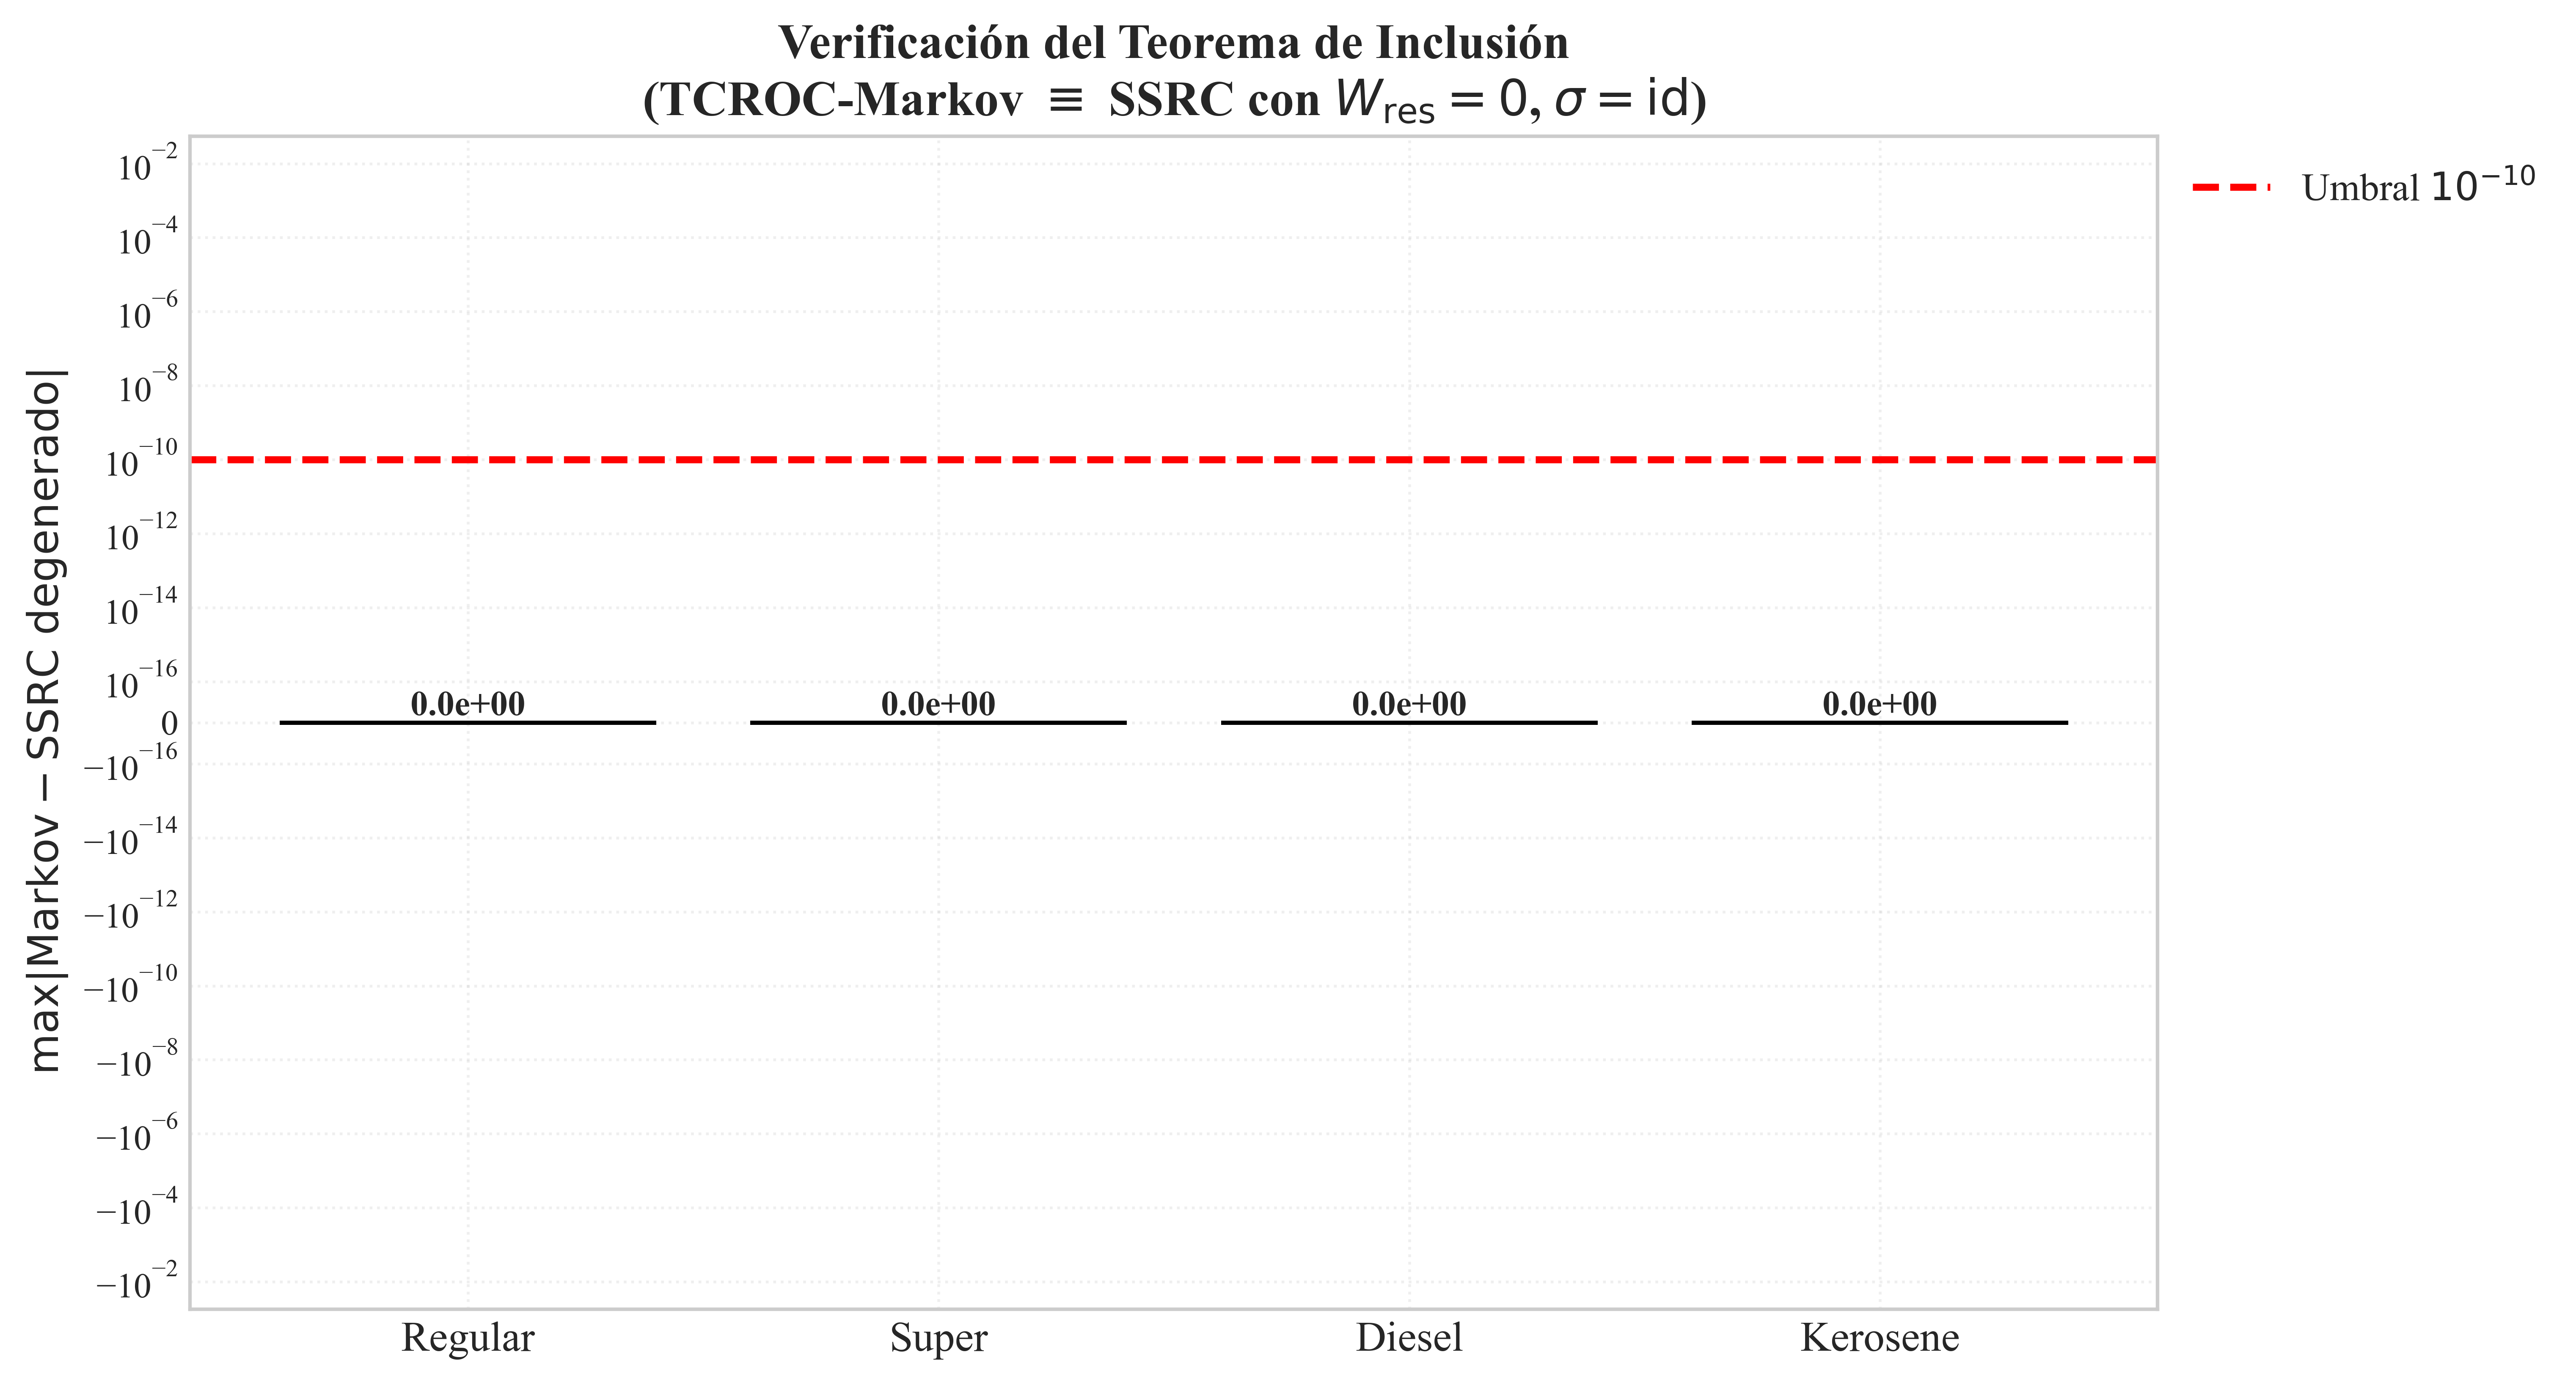
\includegraphics[width=0.95\textwidth]{figures/02_inclusion_theorem.png}
\caption{Verificación de la identidad algebraica entre TCROC-Markov y SSRC degenerado.}
\label{fig:ssrc_inclusion}
\end{figure}

La Figura~\ref{fig:ssrc_inclusion} muestra la verificación numérica del teorema de 
inclusión. Se contrastan las salidas del modelo lineal de Markov con las de 
un reservorio configurado con matriz nula y activación identidad. 
El error residual de exactamente $0.0$ confirma que el marco lineal 
es un subconjunto estricto de la arquitectura SSRC, validando la consistencia 
algebraica de la generalización no lineal propuesta.

\begin{corollary}[Jerarquía de modelos]
\label{cor:jerarquia}
El marco TCROC-Markov del
Capítulo~\ref{cap:regimenes_combustibles} es un caso particular
del SSRC (Definición~\ref{def:ssrc}) obtenido al fijar
$\mat{W}_{\text{res}} = \mat{0}$, $\sigma = \mathrm{id}$,
$a = 1$ y $D = K$.  La extensión a $\mat{W}_{\text{res}} \ne \mat{0}$,
$\sigma = \tanh$, $a < 1$ y $D > K$ constituye una generalización
estrictamente más expresiva: por el
Teorema~\ref{teo:aproximacion_universal}, el SSRC puede aproximar
cualquier funcional causal continuo sobre secuencias, mientras que
TCROC-Markov está restringido a dependencias lineales sobre estados
discretos de un paso.
\end{corollary}

\begin{proof}
La primera afirmación es consecuencia directa del
Teorema~\ref{teo:inclusion}.  Para la segunda, basta observar que
el conjunto de funciones realizables por TCROC-Markov (composiciones
lineales de indicadoras de pertenencia a clústeres) es un subconjunto
propio del conjunto de funcionales continuos sobre
$\set{U}^{\mathbb{Z}_{-}}$.  La densidad del segundo en la
topología del producto está garantizada por el
Teorema~\ref{teo:aproximacion_universal}.
\end{proof}

% --- SECCIÓN: Estimación de la Capa de Lectura vía NNLS ---
\section{Estimación de la Capa de Lectura vía NNLS}
\label{sec:ssrc_estimacion_nnls}
% ===================================================================

La separación entre reservorio fijo y lectura entrenable permite
reducir la estimación de $\mat{W}_{\text{out}}$ a un problema de
mínimos cuadrados, que en nuestro caso resolvemos bajo la restricción de no negatividad para asegurar que se optimiza siempre de forma positiva y no negativa, lo cual es axiomático para que el vector actúe como una suma convexa de propiedades físicas sin cancelar filtros.

% --- SUBSECCIÓN: Formulación del Problema --- - - - - - - - - - - - - - - - - - - - - - - - - - - - - - -
\subsection{Formulación del Problema}
\label{subsec:formulacion_nnls_ssrc}
% -------------------------------------------------------------------

Dada la secuencia de estados del reservorio
$\{\vect{h}_t\}_{t=W}^{T}$ generada por la señal TCROC
$\{\alpha_t\}$, y los valores objetivo
$\{y_t\}_{t=W+1}^{T}$, se busca la matriz de lectura que
minimiza el error de reconstrucción:
\begin{equation}
    \hat{\mat{W}}_{\text{out}} = \argmin_{\mat{W} \ge \mat{0}}
    \sum_{t=W}^{T-1}
    \|y_{t+1} - \mat{W}\,\vect{h}_t\|^2.
    \label{eq:nnls_ssrc}
\end{equation}

Definiendo la matriz de estados acumulados
$\mat{H} = [\vect{h}_W, \vect{h}_{W+1}, \ldots,
\vect{h}_{T-1}] \in \mathbb{R}^{D \times (T-W)}$ y el vector
de objetivos $\vect{y} = [y_{W+1}, \ldots, y_T]^T$, el
problema~\eqref{eq:nnls_ssrc} se reescribe en forma matricial:
\begin{equation}
    \hat{\vect{w}} = \argmin_{\vect{w} \ge \vect{0}}
    \|\vect{y} - \mat{H}^T\vect{w}\|^2,
    \label{eq:nnls_ssrc_matricial}
\end{equation}
donde $\vect{w} = \text{vec}(\mat{W}_{\text{out}}^T)$.

% --- SUBSECCIÓN: Herencia de las Propiedades NNLS --- - - - - - - - - - - - - - - - - - - - - - - - - - - - - - -
\subsection{Herencia de las Propiedades NNLS}
\label{subsec:herencia_nnls}
% -------------------------------------------------------------------

\begin{theorem}[Existencia y unicidad de la capa de lectura NNLS]
\label{teo:existencia_wout}
Sea $\mat{H} \in \mathbb{R}^{D \times (T-W)}$ la matriz de estados
del reservorio.  Entonces:
\begin{enumerate}
    \item \textbf{Existencia:} El
    problema~\eqref{eq:nnls_ssrc_matricial} admite al menos una
    solución.
    \item \textbf{Unicidad:} Si $\mat{H}$ tiene rango completo por
    filas (i.e., $\mathrm{rango}(\mat{H}) = D$), la solución es
    única.
\end{enumerate}
\end{theorem}

\begin{proof}
\textbf{(1) Existencia.}  El conjunto factible
$\set{C} = \{\vect{w} \in \mathbb{R}^{Dm} : \vect{w} \ge \vect{0}\}$
es un cono convexo cerrado no vacío ($\vect{0} \in \set{C}$).  La
función objetivo $f(\vect{w}) = \|\vect{y} - \mat{H}^T\vect{w}\|^2$
es continua y coerciva en $\set{C}$.  Por el teorema de
Weierstrass, $f$ alcanza su mínimo en $\set{C}$.

\textbf{(2) Unicidad.}  Si $\mathrm{rango}(\mat{H}) = D$, entonces
$\mat{H}\mat{H}^T$ es definida positiva, lo que implica que
$f(\vect{w}) = \vect{w}^T(\mat{H}\mat{H}^T)\vect{w} -
2\vect{y}^T\mat{H}^T\vect{w} + \|\vect{y}\|^2$ es estrictamente
convexa en $\vect{w}$.  Un funcional estrictamente convexo sobre un
conjunto convexo tiene a lo sumo un minimizador.  Combinado con la
existencia del punto (1), la solución es única.
\end{proof}

\begin{remark}[Condición de rango y condicionamiento numérico]
\label{obs:condicion_rango}
La condición $\mathrm{rango}(\mat{H}) = D$ requiere $T - W \ge D$ y
que los estados del reservorio sean linealmente independientes.  La no
linealidad de $\tanh$ y la aleatoriedad de
$\mat{W}_{\text{in}}, \mat{W}_{\text{res}}$ garantizan que esta
condición se satisface genéricamente cuando $T - W > D$.  Sin embargo,
la \emph{unicidad teórica} no implica \emph{estabilidad numérica}:
si el número de condición $\kappa(\mat{H}) = \sigma_{\max}/\sigma_{\min}$
es grande, la solución NNLS puede ser sensible a perturbaciones en
los datos.  En la práctica, la restricción de no negatividad del NNLS
actúa como una regularización implícita que mitiga parcialmente este
efecto, y el promediado sobre múltiples realizaciones
(\textit{ensemble}) lo reduce adicionalmente.  El análisis empírico
del condicionamiento se presenta en la
Sección~\ref{subsec:verificaciones_teoricas}.
\end{remark}

% --- SECCIÓN: Arquitectura TCROC-SSRC ---
\section{Arquitectura TCROC-SSRC}
\label{sec:arquitectura_tcroc_ssrc}
% ===================================================================

La Figura~\ref{fig:ssrc_architecture} presenta la comparación
esquemática de ambas arquitecturas, evidenciando que los pasos 1--2
(extracción TCROC) y 4 (estimación NNLS) son compartidos; la
diferencia reside exclusivamente en el paso 3: discretización K-Means
en TCROC-Markov vs.\ proyección al reservorio recurrente en
TCROC-SSRC.

\begin{figure}[H]
\centering
\includegraphics[width=0.95\textwidth]{figures/01_architecture_diagram.png}
\caption{Comparación esquemática de las arquitecturas TCROC-Markov y TCROC-SSRC.}
\label{fig:ssrc_architecture}
\end{figure}

Como se detalla en el diagrama de la Figura~\ref{fig:ssrc_architecture}, 
ambos marcos tecnológicos comparten la fase inicial de extracción de 
características y la fase final de estimación por mínimos cuadrados. 
La distinción radica en el procesamiento de la información en el espacio de estados, 
donde el modelo SSRC sustituye la discretización por clústeres por una proyección
 a un espacio continuo recurrente de alta dimensión, permitiendo capturar 
 dependencias temporales no lineales inaccesibles para el modelo lineal.

\begin{definition}[Marco TCROC-SSRC]
\label{def:marco_tcroc_ssrc}
El \textbf{marco TCROC-SSRC} para pronóstico de series temporales
consiste en el flujo secuencial:
\begin{enumerate}
    \item \textbf{Extracción TCROC:} Dada la serie $\{v_t\}$, se
    computa la señal $\alpha_t = \alpha_t(W, \lambda)$ según la
    ecuación~\eqref{eq:alpha_t_combustibles} del
    Capítulo~\ref{cap:regimenes_combustibles}.
    \item \textbf{Proyección al reservorio:} Se define la entrada
    $u_t = \alpha_t \in \mathbb{R}$ y se propaga mediante la
    ecuación Leaky-ESN~\eqref{eq:leaky_esn}, con $\vect{h}_0 = \vect{0}$
    y los primeros $W_{\text{wash}}$ pasos descartados
    (\textit{washout}) para eliminar transitorios.
    \item \textbf{Estimación de lectura:} Se resuelve el problema
    NNLS~\eqref{eq:nnls_ssrc} para obtener
    $\hat{\mat{W}}_{\text{out}}$.
    \item \textbf{Pronóstico:} El valor predicho es
    $\hat{y}_{t+1} = \hat{\mat{W}}_{\text{out}}\,\vect{h}_t$.
\end{enumerate}
Los hiperparámetros del marco son: $(W, \lambda)$ heredados de TCROC;
$(D, \rho_{\text{res}}, a, W_{\text{wash}})$ propios del reservorio.
\end{definition}

\begin{proposition}[Consistencia con el caso lineal]
\label{prop:consistencia_lineal}
Con los hiperparámetros del reservorio fijados en
$D = K$, $\mat{W}_{\text{res}} = \mat{0}$, $\sigma = \mathrm{id}$,
$a = 1$ y $W_{\text{wash}} = 0$, el marco TCROC-SSRC se reduce
exactamente al marco TCROC-Markov del
Capítulo~\ref{cap:regimenes_combustibles}.
\end{proposition}

\begin{proof}
Consecuencia directa del Teorema~\ref{teo:inclusion}.
\end{proof}

% --- SECCIÓN: Propiedades de Estabilidad del Pronóstico ---
\section{Propiedades de Estabilidad del Pronóstico}
\label{sec:ssrc_estabilidad}
% ===================================================================

\begin{proposition}[Acotación del error de pronóstico]
\label{prop:acotacion_error}
Sea $\hat{y}_{t+1} = \hat{\mat{W}}_{\text{out}}\,\vect{h}_t$ el
pronóstico del SSRC.  Si el reservorio satisface la ESP con
$\rho(\mat{W}_{\text{res}}) = \rho_{\text{res}} < 1$, entonces
para toda perturbación $\delta\vect{u}_t$ en la entrada con
$\|\delta\vect{u}_t\| \le \epsilon$, la perturbación inducida en
la salida satisface:
\begin{equation}
    \|\delta \hat{y}_{t+1}\| \le
    \|\hat{\mat{W}}_{\text{out}}\|\,
    \frac{\|\mat{W}_{\text{in}}\|\,\epsilon}
    {1 - \rho_{\text{res}}}.
    \label{eq:acotacion_perturbacion}
\end{equation}
\end{proposition}

\begin{proof}
Sea $\{\vect{h}_t\}$ la trayectoria nominal y
$\{\vect{h}_t + \delta\vect{h}_t\}$ la trayectoria perturbada.
Por la Lipschitz continuidad de $\tanh$ con constante $L = 1$:
\begin{equation}
    \|\delta\vect{h}_t\| \le
    \|\mat{W}_{\text{in}}\|\,\|\delta\vect{u}_t\| +
    \|\mat{W}_{\text{res}}\|\,\|\delta\vect{h}_{t-1}\|.
\end{equation}
Si la perturbación es sostenida con
$\|\delta\vect{u}_t\| \le \epsilon$ para todo $t$, iterando
la desigualdad y sumando la serie geométrica:
\begin{equation}
    \sup_t \|\delta\vect{h}_t\| \le
    \frac{\|\mat{W}_{\text{in}}\|\,\epsilon}
    {1 - \rho_{\text{res}}}.
\end{equation}
La cota sobre la salida sigue de la linealidad de la lectura:
$\|\delta\hat{y}_{t+1}\| \le \|\hat{\mat{W}}_{\text{out}}\|\,
\|\delta\vect{h}_t\|$.
\end{proof}

\begin{remark}[Conservadurismo de la cota]
\label{obs:cota_conservadora}
La cota~\eqref{eq:acotacion_perturbacion} es una \emph{cota en el
peor caso} que puede ser significativamente conservadora.  En la
práctica, $\|\hat{\mat{W}}_{\text{out}}\|$ depende fuertemente
del condicionamiento de $\mat{H}$: números de condición altos
producen normas $\|\hat{\mat{W}}_{\text{out}}\|$ grandes,
inflando la cota sin que esto se traduzca necesariamente en
inestabilidad observable.  La restricción de no negatividad del NNLS
restringe $\hat{\mat{W}}_{\text{out}}$ al ortante positivo,
proporcionando una forma de regularización implícita que la cota
teórica no captura.  El análisis empírico de la
Sección~\ref{subsec:sensibilidad_hiperparametros} muestra que la
variabilidad real del pronóstico es órdenes de magnitud menor que
la cota teórica.
\end{remark}

% --- SECCIÓN: Aplicación Comparativa: Combustibles Hondureños ---
\section{Aplicación Comparativa: Combustibles Hondureños}
\label{sec:ssrc_aplicacion}

% --- SUBSECCIÓN: Configuración Experimental --- - - - - - - - - - - - - - - - - - - - - - - - - - - - - - -
\subsection{Configuración Experimental}
\label{subsec:ssrc_configuracion}
% -------------------------------------------------------------------

Los hiperparámetros TCROC se fijaron en los valores óptimos
identificados en la Tabla~\ref{tab:hiperparametros_optimos} del
capítulo anterior.  Para el reservorio, se evaluó una búsqueda
exhaustiva en grilla sobre tres hiperparámetros:
\begin{align}
    D &\in \{20, 30, 40, 50, 60, 75, 100, 150\}, \nonumber\\
    \rho_{\text{res}} &\in \{0.70, 0.80, 0.85, 0.90, 0.95, 0.99\}, \quad
    a \in \{0.1, 0.3, 0.5, 0.7, 1.0\},
    \label{eq:grilla_ssrc}
\end{align}
totalizando $8 \times 6 \times 5 = 240$ configuraciones por serie.
Se fijaron $\omega = 1.0$ para la escala de $\mat{W}_{\text{in}}$,
dispersión del 90\% en $\mat{W}_{\text{res}}$, y
$W_{\text{wash}} = 50$ pasos de washout.  Para cada celda de la
grilla, se evaluaron 5 realizaciones independientes de las matrices
aleatorias, seleccionando el mejor $(D^*, \rho^*, a^*)$ por RMSE
medio.  La evaluación final de la configuración óptima se realizó
con un ensemble de 30 realizaciones independientes para obtener
estimaciones robustas de la media y la variabilidad.

% --- SUBSECCIÓN: Verificaciones Teóricas --- - - - - - - - - - - - - - - - - - - - - - - - - - - - - - -
\subsection{Verificaciones Teóricas}
\label{subsec:verificaciones_teoricas}
% -------------------------------------------------------------------

Antes de reportar los resultados predictivos, se verificaron las
condiciones teóricas establecidas en las secciones precedentes.  La
Tabla~\ref{tab:verificaciones_teoricas} resume los resultados para
la configuración óptima de cada serie.

\begin{table}[H]
\centering
\caption{Verificación de las condiciones teóricas del SSRC.}
\label{tab:verificaciones_teoricas}
\begin{tabular}{@{}lcccccc@{}}
\toprule
\textbf{Serie} & $D^*$ & $\rho^*$ 
& \textbf{ESP} & $\mathrm{rango}(\mat{H})$ & $T_{\text{eff}}$
& $\kappa(\mat{H})$ \\
\midrule
Regular  & 150 & 0.85 & Sí & 150 & 340 &
$1.47 \times 10^{9}$ \\
Súper    & 150 & 0.70 & Sí & 150 & 338 &
$5.60 \times 10^{10}$ \\
Diésel   & 150 & 0.80 & Sí & 150 & 340 &
$3.28 \times 10^{9}$ \\
Kerosene &  60 & 0.70 & Sí &  60 & 338 &
$1.14 \times 10^{9}$ \\
\bottomrule
\end{tabular}
\end{table}

Las cuatro configuraciones satisfacen la ESP (todos los
$\rho^* < 1$) y la condición de rango completo
($\mathrm{rango}(\mat{H}) = D^*$ en todos los casos).  La
Figura~\ref{fig:ssrc_eigenvalues} visualiza el espectro de
$\mat{W}_{\text{res}}$, confirmando que todos los autovalores se
encuentran estrictamente dentro del círculo unitario.

\begin{figure}[H]
\centering
\includegraphics[width=0.95\textwidth]{figures/04_eigenvalues_complex_plane.png}
\caption{Autovalores de $\mat{W}_{\text{res}}$ en el plano complejo.}
\label{fig:ssrc_eigenvalues}
\end{figure}

La Figura~\ref{fig:ssrc_eigenvalues} muestra los autovalores de 
$\mat{W}_{\text{res}}$ para la configuración óptima de cada serie. 
El círculo negro punteado representa el círculo unitario ($|z| = 1$), 
mientras que el círculo rojo sólido indica el radio espectral objetivo 
$\rho^*$. Se verifica que todos los autovalores se encuentran estrictamente 
dentro del círculo unitario, cumpliendo con la condición suficiente para la 
ESP detallada en el Teorema~\ref{teo:esp_suficiente}. Los radios espectrales 
óptimos moderados ($\rho^* \in [0.70, 0.85]$) indican que el reservorio no 
requiere de memoria máxima para capturar la dinámica de los combustibles.

Los números de condición $\kappa(\mat{H})$ merecen discusión
explícita. Los valores observados, que se sitúan en el orden de $10^9$ a
$10^{10}$, indican que la matriz $\mat{H}\mat{H}^T$ está
pobremente condicionada en sentido numérico.  Esto es una
consecuencia directa de la dimensión $D = 150$ combinada con la
naturaleza de la señal $\alpha_t$, que tiene variabilidad reducida
($|\alpha_t| < 0.02$ típicamente).  Sin embargo, tres factores
mitigan este condicionamiento en la práctica: (i) la restricción
$\vect{w} \ge \vect{0}$ del NNLS actúa como una regularización
implícita, restringiendo la solución al ortante positivo y
eliminando las direcciones negativas que amplifican el error;
(ii) el ensemble de 30 realizaciones promedia sobre diferentes
matrices $\mat{W}_{\text{in}}$ y $\mat{W}_{\text{res}}$, cada
una con condicionamiento diferente; y (iii) los resultados
predictivos (Sección~\ref{subsec:ssrc_resultados}) muestran
variabilidad baja entre realizaciones, evidenciando estabilidad
práctica a pesar del condicionamiento teórico adverso.

La convergencia del periodo de washout se presenta en la
Figura~\ref{fig:ssrc_washout}.

\begin{figure}[H]
\centering
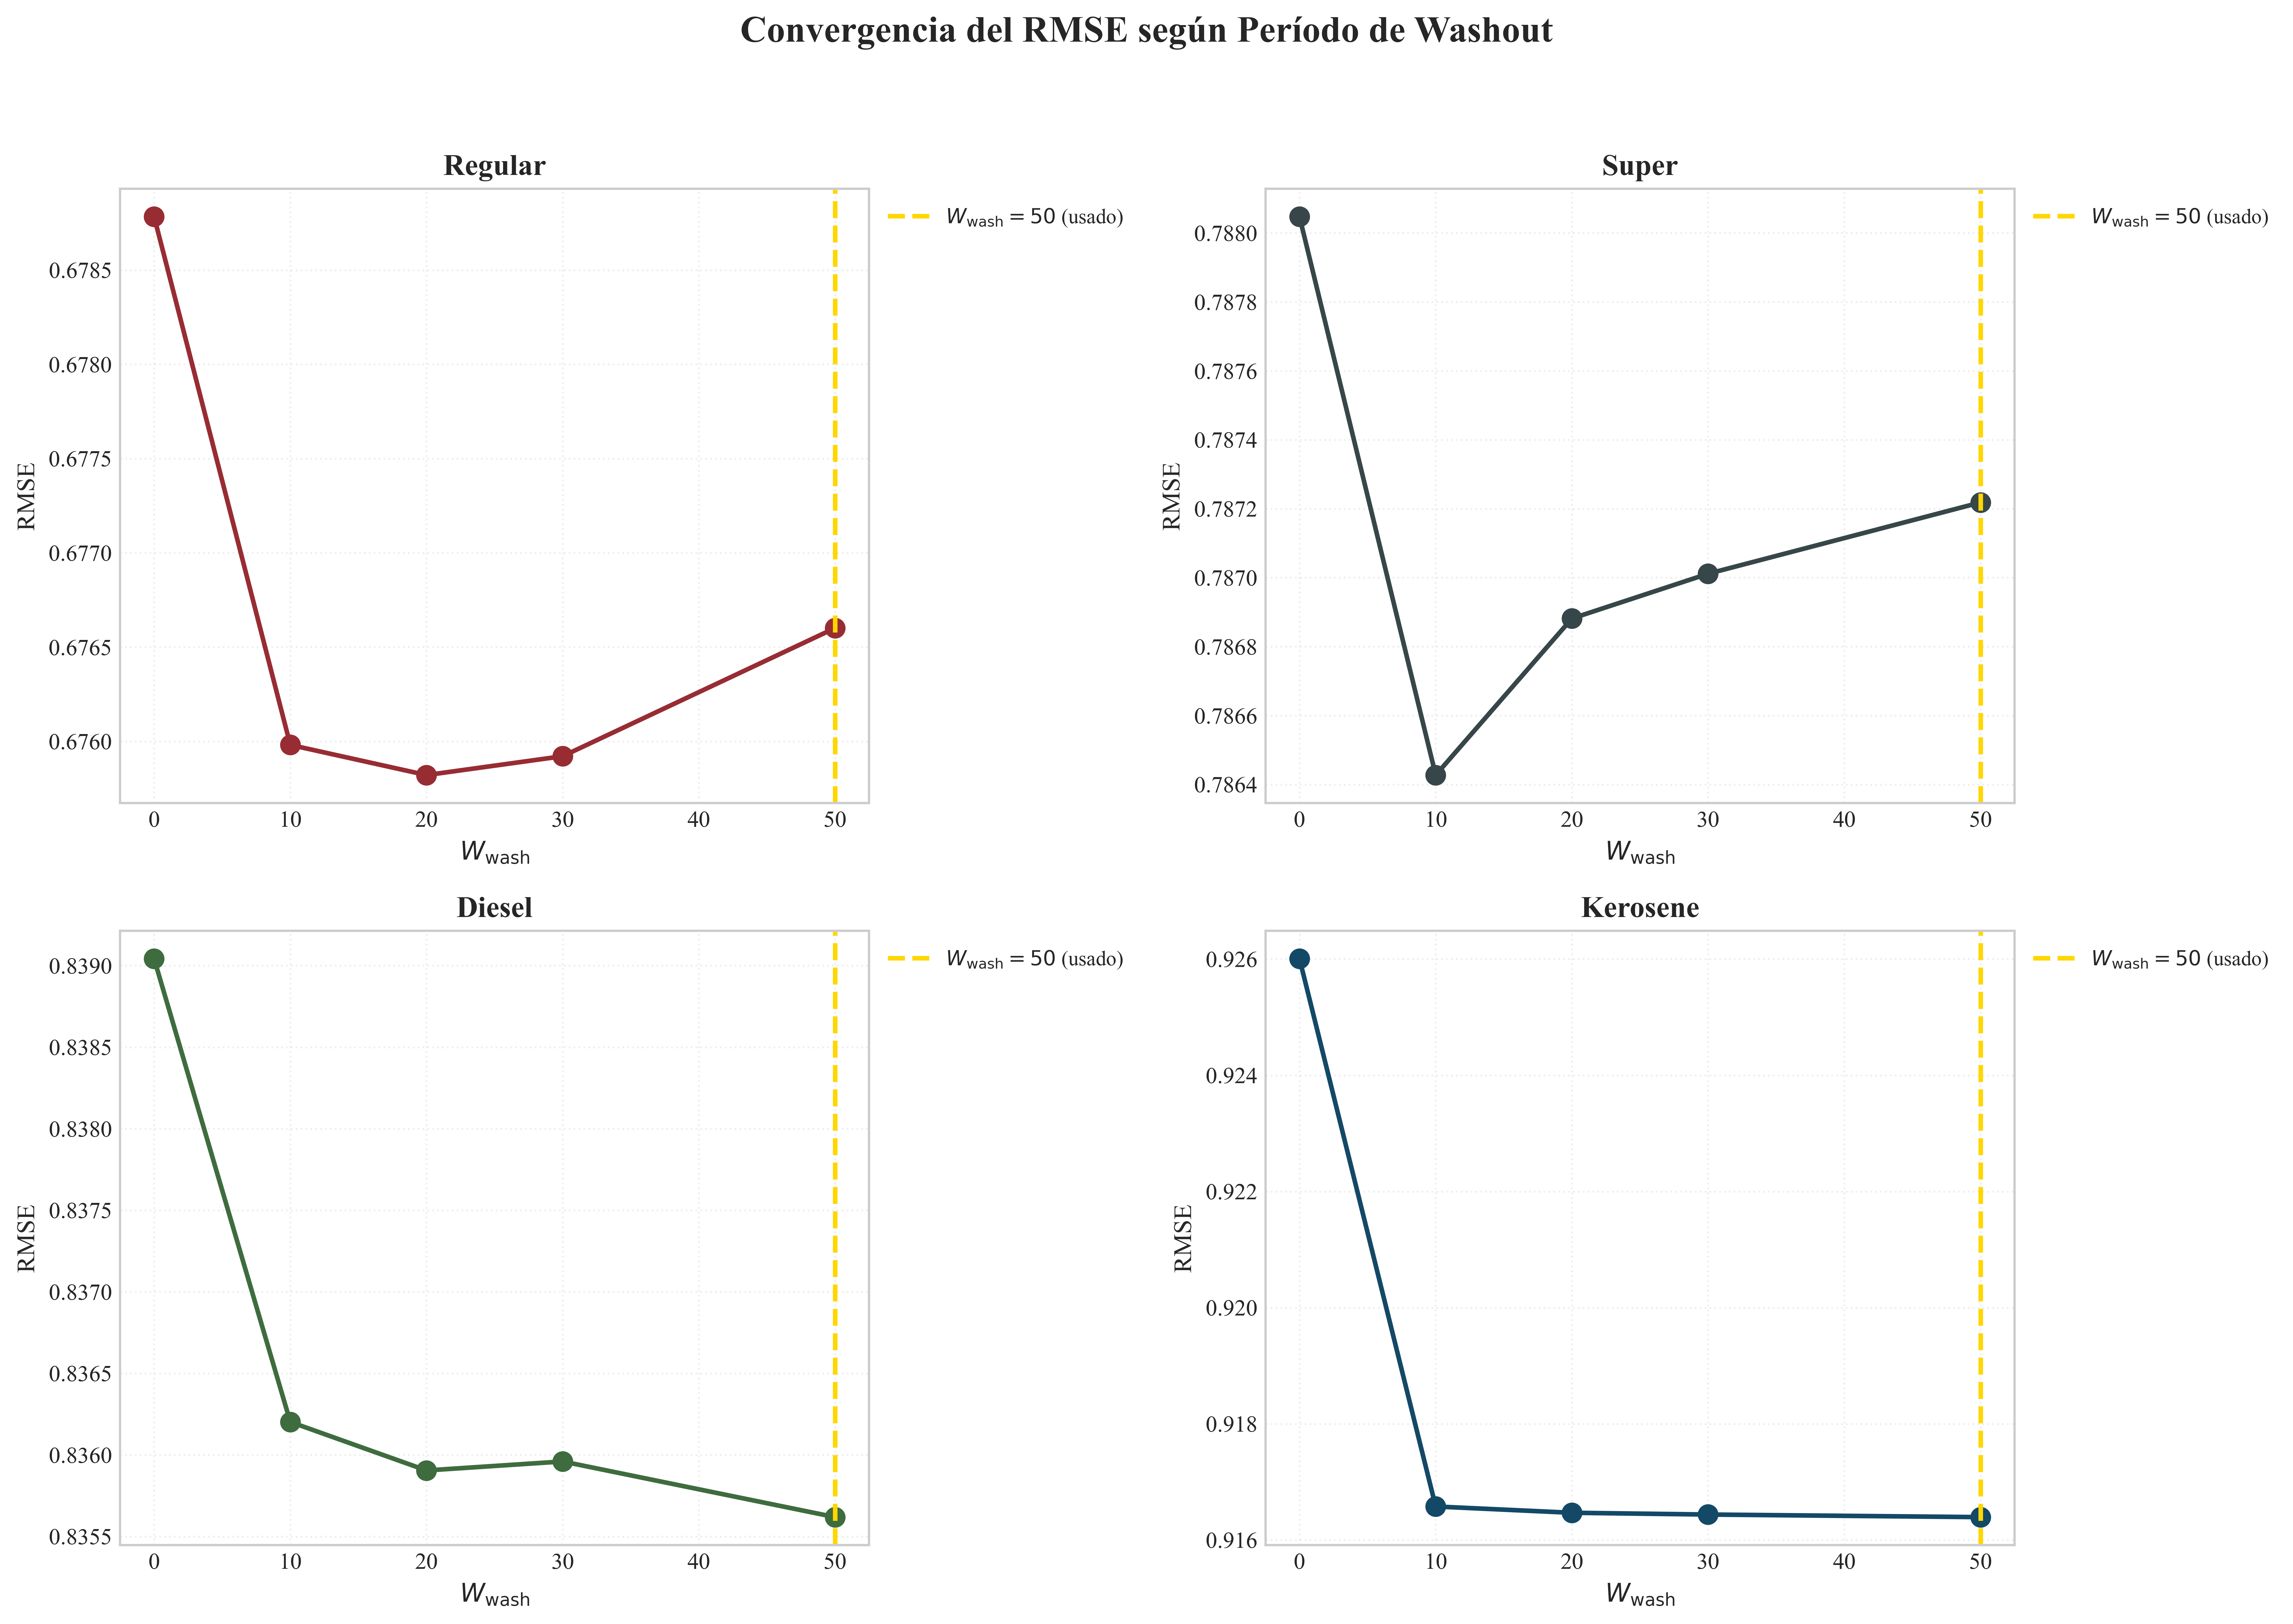
\includegraphics[width=0.95\textwidth]{figures/11_washout_convergence.png}
\caption{Convergencia del RMSE según el periodo de washout $W_{\text{wash}}$.}
\label{fig:ssrc_washout}
\end{figure}

Como se ilustra en la Figura~\ref{fig:ssrc_washout}, el RMSE se estabiliza 
para las cuatro series a partir de un periodo de $W_{\text{wash}} 
\approx 10$--$20$. Esto confirma la eficiencia de la ESP, puesto que la 
influencia de la condición inicial $\vect{h}_0 = \vect{0}$ se disipa rápidamente. 
La línea amarilla punteada señala el valor utilizado de $W_{\text{wash}} = 50$, 
el cual se encuentra dentro de la región de convergencia estable, reflejando el 
decaimiento exponencial rápido asociado a radios espectrales moderados ($\rho^* \le 0.85$).

% --- SUBSECCIÓN: Optimización de Hiperparámetros --- - - - - - - - - - - - - - - - - - - - - - - - - - - - - - -
\subsection{Optimización de Hiperparámetros}
\label{subsec:optimizacion_ssrc}
% -------------------------------------------------------------------

La Figura~\ref{fig:ssrc_heatmap} presenta los resultados de la
búsqueda en grilla como mapas de calor del RMSE medio en el plano
$(D, \rho)$, donde para cada celda se reporta el mejor valor de
$a$ encontrado.

\begin{figure}[H]
\centering
\includegraphics[width=1\textwidth]{figures/03_grid_heatmap.png}
\caption{Búsqueda en grilla del SSRC sobre el plano $(D, \rho)$.}
\label{fig:ssrc_heatmap}
\end{figure}

Los resultados de la búsqueda en grilla presentados en la Figura~\ref{fig:ssrc_heatmap} 
muestran el RMSE medio para cada combinación $(D, \rho)$ y el mejor factor de fuga $a^*$ 
por celda, con el recuadro negro indicando la configuración óptima. Se observa que para Regular,
 Súper y Diésel el óptimo se alcanza en $D = 150$, mientras que para Kerosene ocurre en 
 $D = 60$. Los radios espectrales óptimos son moderados y la superficie de error es suave, 
 manteniendo el RMSE del SSRC significativamente por debajo del modelo Markoviano en todos los paneles.

La Tabla~\ref{tab:hiperparametros_ssrc} resume la configuración
óptima identificada para cada serie.

\begin{table}[H]
\centering
\caption{Hiperparámetros óptimos del SSRC por serie de combustible.}
\label{tab:hiperparametros_ssrc}
\begin{tabular}{@{}lcccccc@{}}
\toprule
\textbf{Serie} & $D^*$ & $\rho^*$ & $a^*$ &
\textbf{NNLS RMSE} & \textbf{Ridge RMSE} &
$\Delta_{\text{solver}}$ \\
\midrule
Regular  & 150 & 0.85 & 0.1 & 0.6595 & 0.6741 & $-2.16\%$ \\
Súper    & 150 & 0.70 & 0.3 & 0.7810 & 0.7885 & $-0.95\%$ \\
Diésel   & 150 & 0.80 & 0.1 & 0.8299 & 0.8443 & $-1.70\%$ \\
Kerosene &  60 & 0.70 & 1.0 & 0.9156 & 0.9173 & $-0.17\%$ \\
\bottomrule
\end{tabular}
\end{table}

Tres observaciones emergen de la optimización.  Primero, los valores
$a^* = 0.1$ para Regular y Diésel indican que el reservorio se
beneficia de una inercia temporal fuerte: el 90\% del estado previo
se preserva en cada paso, actuando como un filtro de suavizado
adaptativo que es consistente con la baja volatilidad semanal de
estos mercados regulados.  Segundo, Kerosene es la única serie con
$a^* = 1.0$ (ESN estándar sin suavizado), coherente con su mayor
volatilidad y complejidad de 5 regímenes identificados en el
capítulo anterior.  Tercero, NNLS supera a Ridge Regression en las
cuatro series, validando empíricamente que la restricción de no
negatividad, la cual garantiza que el pronóstico sea una combinación
positiva de los filtros no lineales del reservorio, aporta
regularización útil.

Las Figuras~\ref{fig:ssrc_sens_D} y~\ref{fig:ssrc_sens_rho}
presentan el análisis de sensibilidad marginal a los hiperparámetros
$D$ y $\rho$, respectivamente.

\begin{figure}[H]
\centering
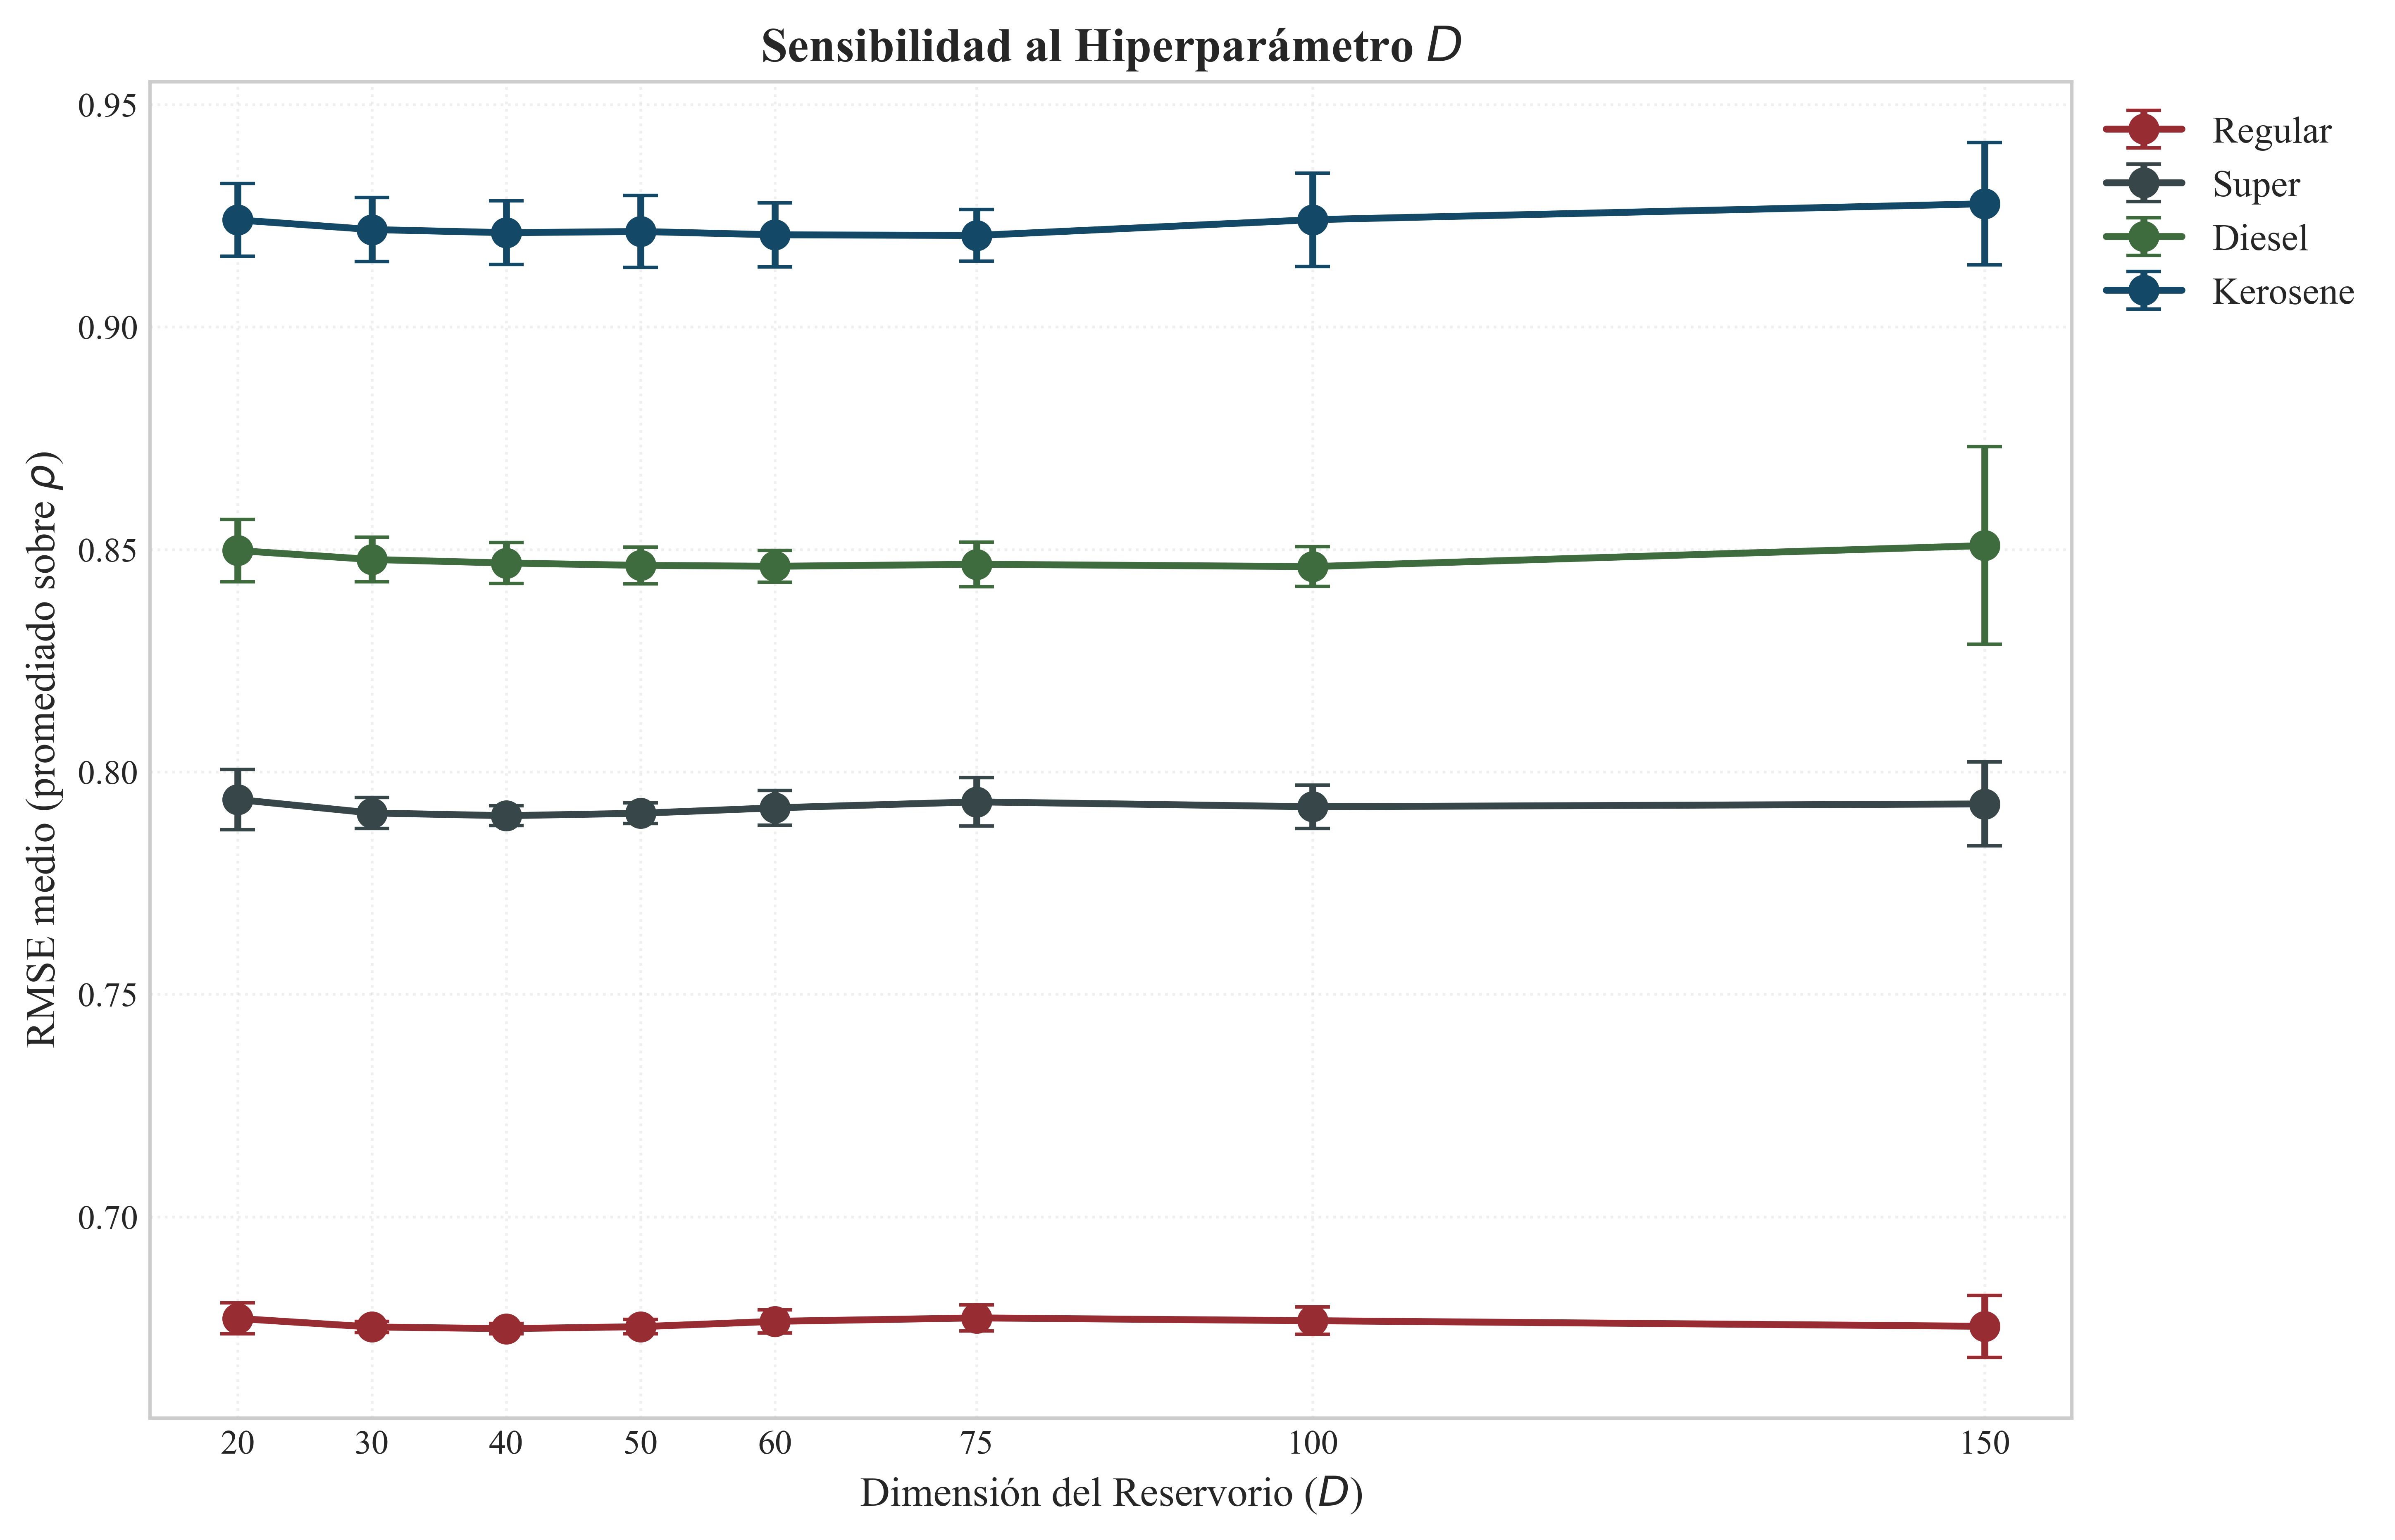
\includegraphics[width=0.95\textwidth]{figures/08_sensitivity_D.png}
\caption{Sensibilidad del RMSE a la dimensión del reservorio $D$.}
\label{fig:ssrc_sens_D}
\end{figure}

La sensibilidad del RMSE respecto a la dimensión $D$ se detalla en la 
Figura~\ref{fig:ssrc_sens_D}. Las curvas promediadas sobre los valores 
de $\rho$ resultan esencialmente planas, con variaciones mínimas entre 
$D = 20$ y $D = 150$. Este comportamiento indica que la complejidad 
no lineal del proceso es baja, permitiendo que incluso dimensiones 
modestas capturen la mayor parte de la estructura, con ganancias 
marginales de apenas el 0.3\% al aumentar la dimensión a los niveles 
máximos evaluados.

\begin{figure}[H]
\centering
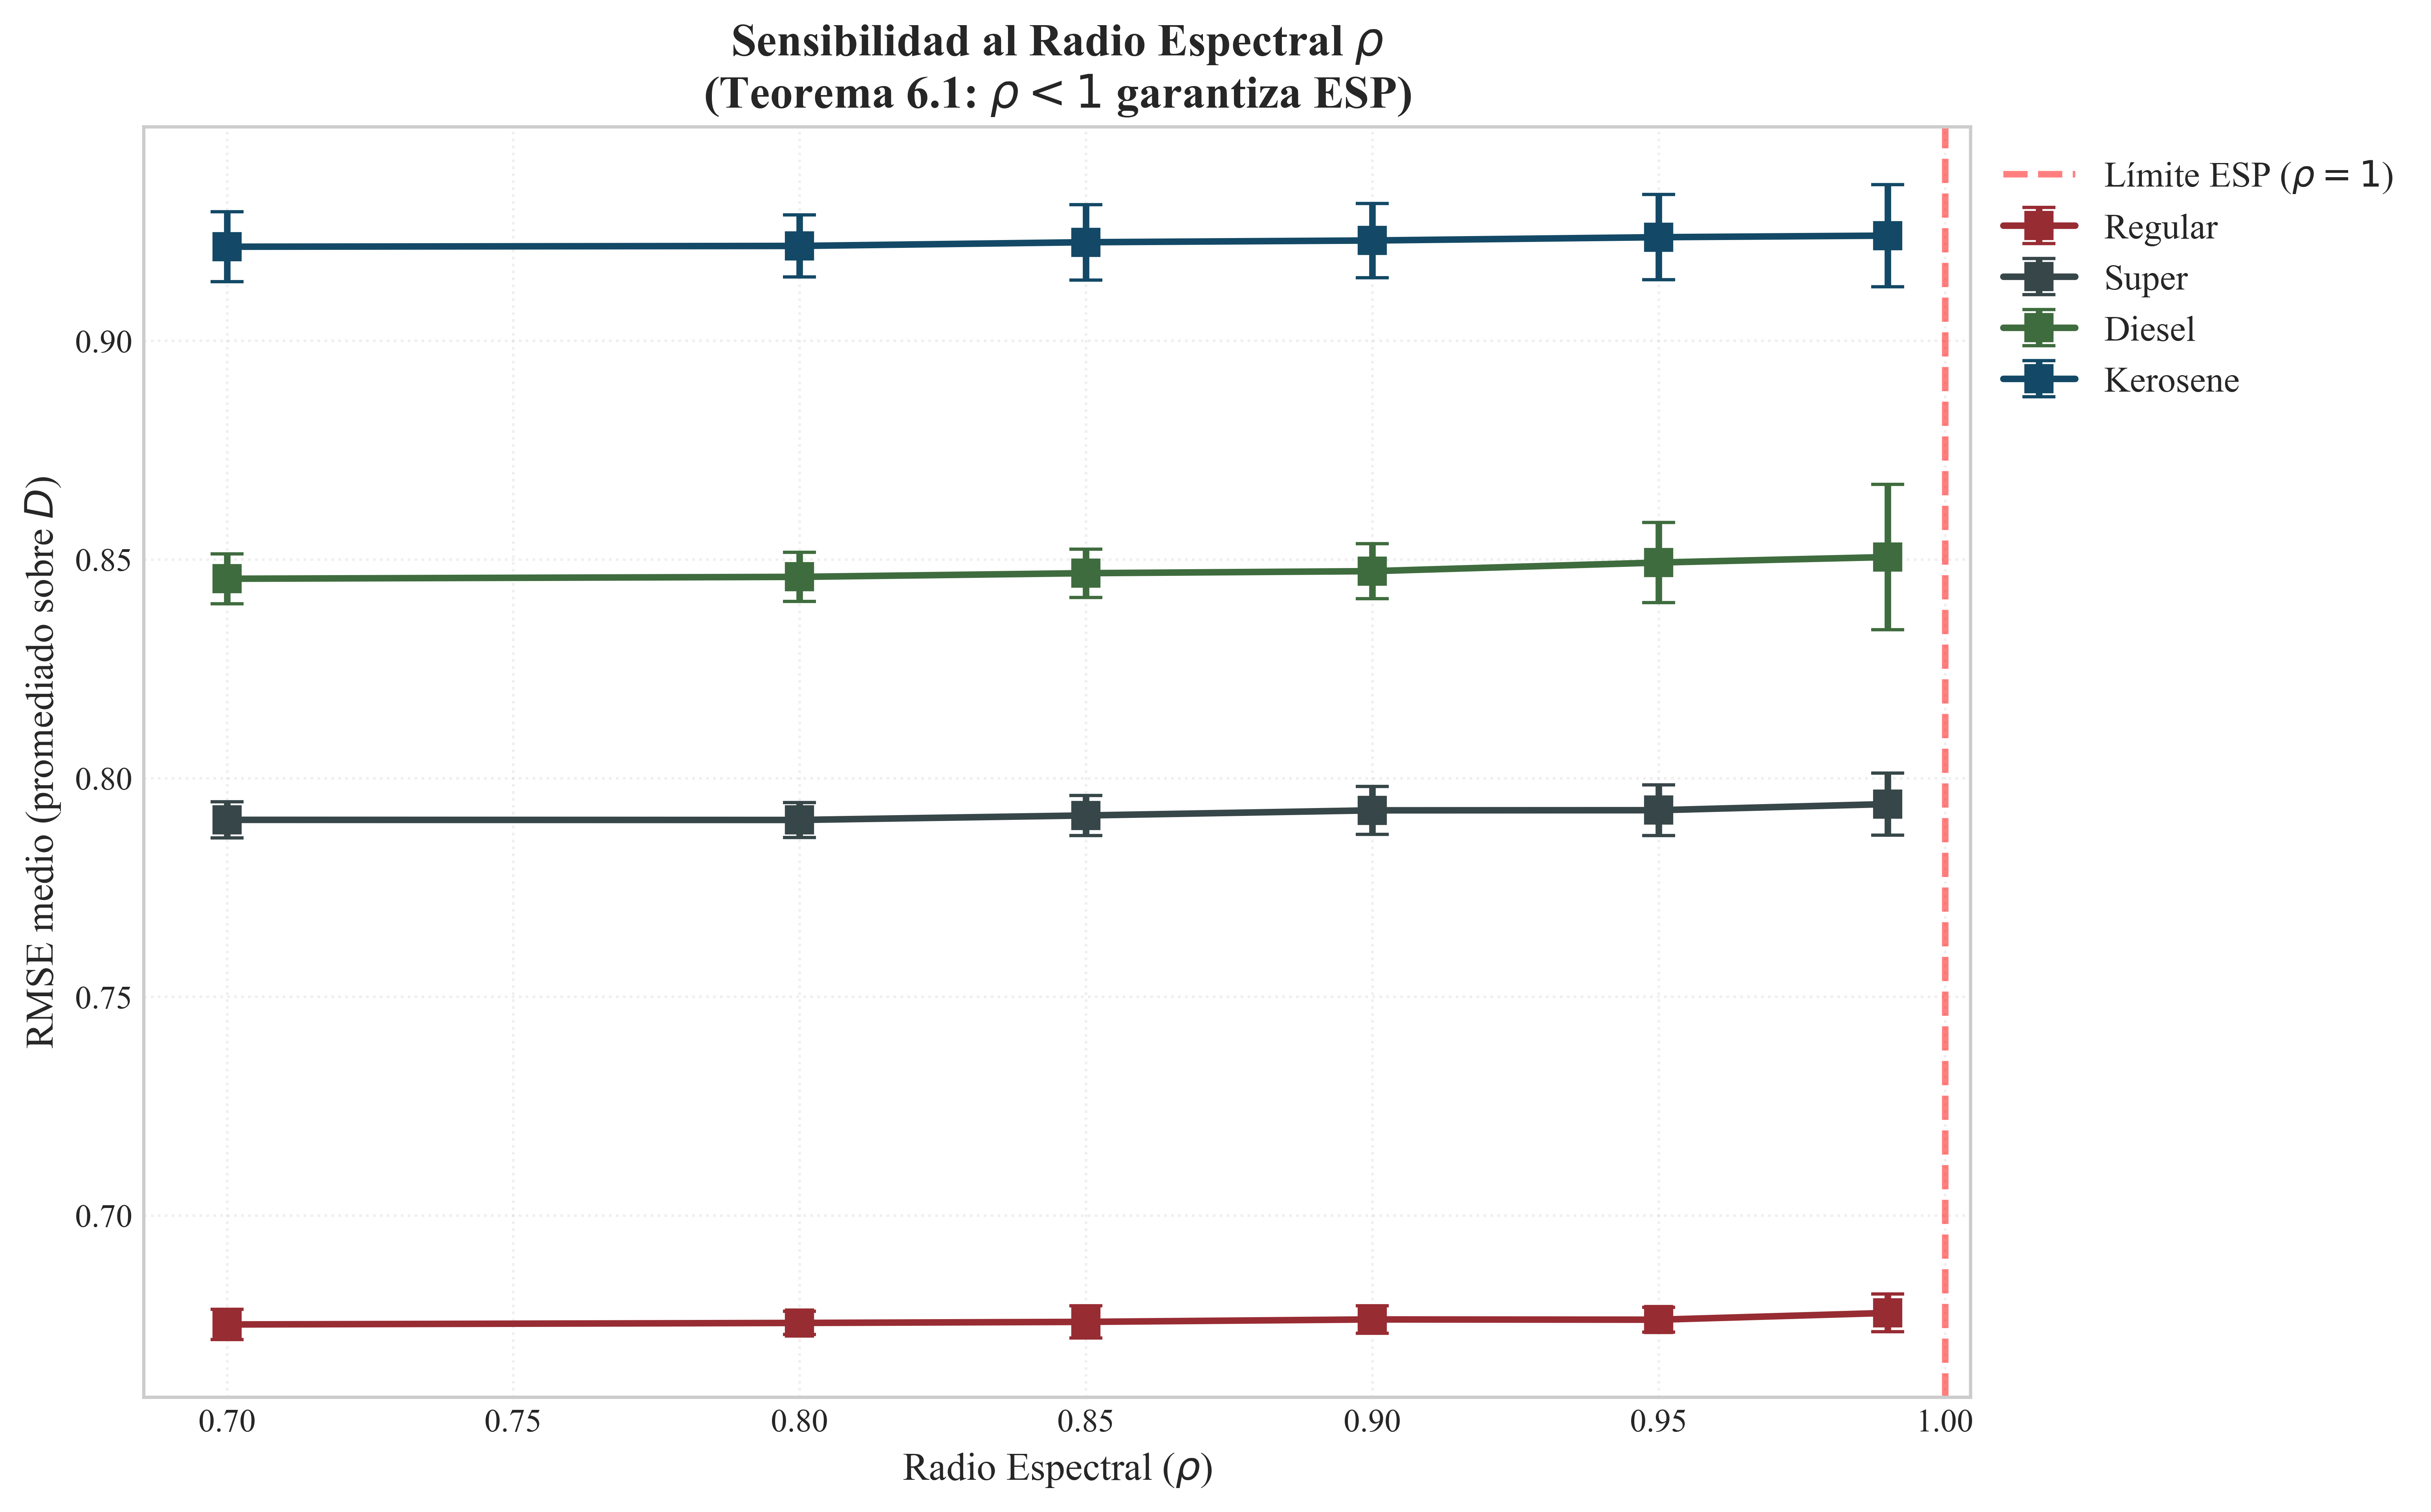
\includegraphics[width=0.95\textwidth]{figures/09_sensitivity_rho.png}
\caption{Sensibilidad del RMSE al radio espectral $\rho$.}
\label{fig:ssrc_sens_rho}
\end{figure}

La Figura~\ref{fig:ssrc_sens_rho} muestra la sensibilidad del RMSE frente 
al radio espectral $\rho$. La tendencia ligeramente creciente hacia 
$\rho = 0.99$ sugiere que un exceso de memoria no lineal no beneficia a 
estas series. Los valores óptimos moderados identificados son consistentes 
con una dinámica dominada por tendencias de largo plazo que ya han sido 
capturadas eficazmente por el operador TCROC.

% --- SUBSECCIÓN: Resultados --- - - - - - - - - - - - - - - - - - - - - - - - - - - - - - -
\subsection{Resultados}
\label{subsec:ssrc_resultados}
% -------------------------------------------------------------------

La Tabla~\ref{tab:comparacion_ssrc} presenta la comparación directa
entre TCROC-Markov y TCROC-SSRC.  La significancia estadística se
evaluó mediante el test de Diebold-Mariano (DM) \cite{dieboldmariano1995},
que compara las secuencias de errores cuadráticos de ambos modelos
bajo la hipótesis nula de igual precisión predictiva.

\begin{table}[H]
\centering
\caption{Comparación de desempeño predictivo: TCROC-Markov vs.\ TCROC-SSRC.}
\label{tab:comparacion_ssrc}
\resizebox{\textwidth}{!}{%
\begin{tabular}{@{}lcccccc@{}}
\toprule
\textbf{Serie} & \textbf{TCROC-Markov} &
\textbf{TCROC-SSRC} & $(D^*, \rho^*, a^*)$ &
$\Delta$\textbf{RMSE} & $p_{\text{DM}}$ &
\textbf{Significativo} \\
\midrule
Regular  & $0.8394$ & $0.6595 \pm 0.013$ &
$(150,\; 0.85,\; 0.1)$ & $-21.43\%$ & $0.1154$ & No \\
Súper    & $0.9769$ & $0.7810 \pm 0.006$ &
$(150,\; 0.70,\; 0.3)$ & $-20.05\%$ & $0.0018$ & Sí \\
Diésel   & $1.0816$ & $0.8299 \pm 0.018$ &
$(150,\; 0.80,\; 0.1)$ & $-23.27\%$ & $0.0326$ & Sí \\
Kerosene & $1.1714$ & $0.9156 \pm 0.005$ &
$(60,\;\, 0.70,\; 1.0)$ & $-21.84\%$ & $0.0061$ & Sí \\
\bottomrule
\end{tabular}%
}
\end{table}

La Tabla~\ref{tab:comparacion_ssrc} presenta la comparación de desempeño predictivo entre TCROC-Markov (lineal) y TCROC-SSRC (no lineal). Se reporta el RMSE fuera de muestra como la media y desviación estándar sobre 30 realizaciones para la extensión SSRC. La significancia estadística, evaluada mediante el test de Diebold-Mariano (DM), muestra que un valor de $p < 0.05$ indica una superioridad significativa del modelo SSRC sobre el benchmark lineal.

El TCROC-SSRC reduce el RMSE entre un 20\% y un 23\% respecto
al modelo Markoviano en las cuatro series.  La mejora es
estadísticamente significativa al nivel $\alpha = 0.05$ para Súper
($p = 0.002$), Diésel ($p = 0.033$) y Kerosene ($p = 0.006$).
Para Regular, la mejora es sustancial en magnitud ($-21.43\%$) pero
marginalmente significativa ($p = 0.115$); esto se atribuye a la
menor varianza de los errores de Regular (la serie más predecible),
que reduce la potencia del test DM.

La Figura~\ref{fig:ssrc_barplot} visualiza esta comparación.

\begin{figure}[H]
\centering
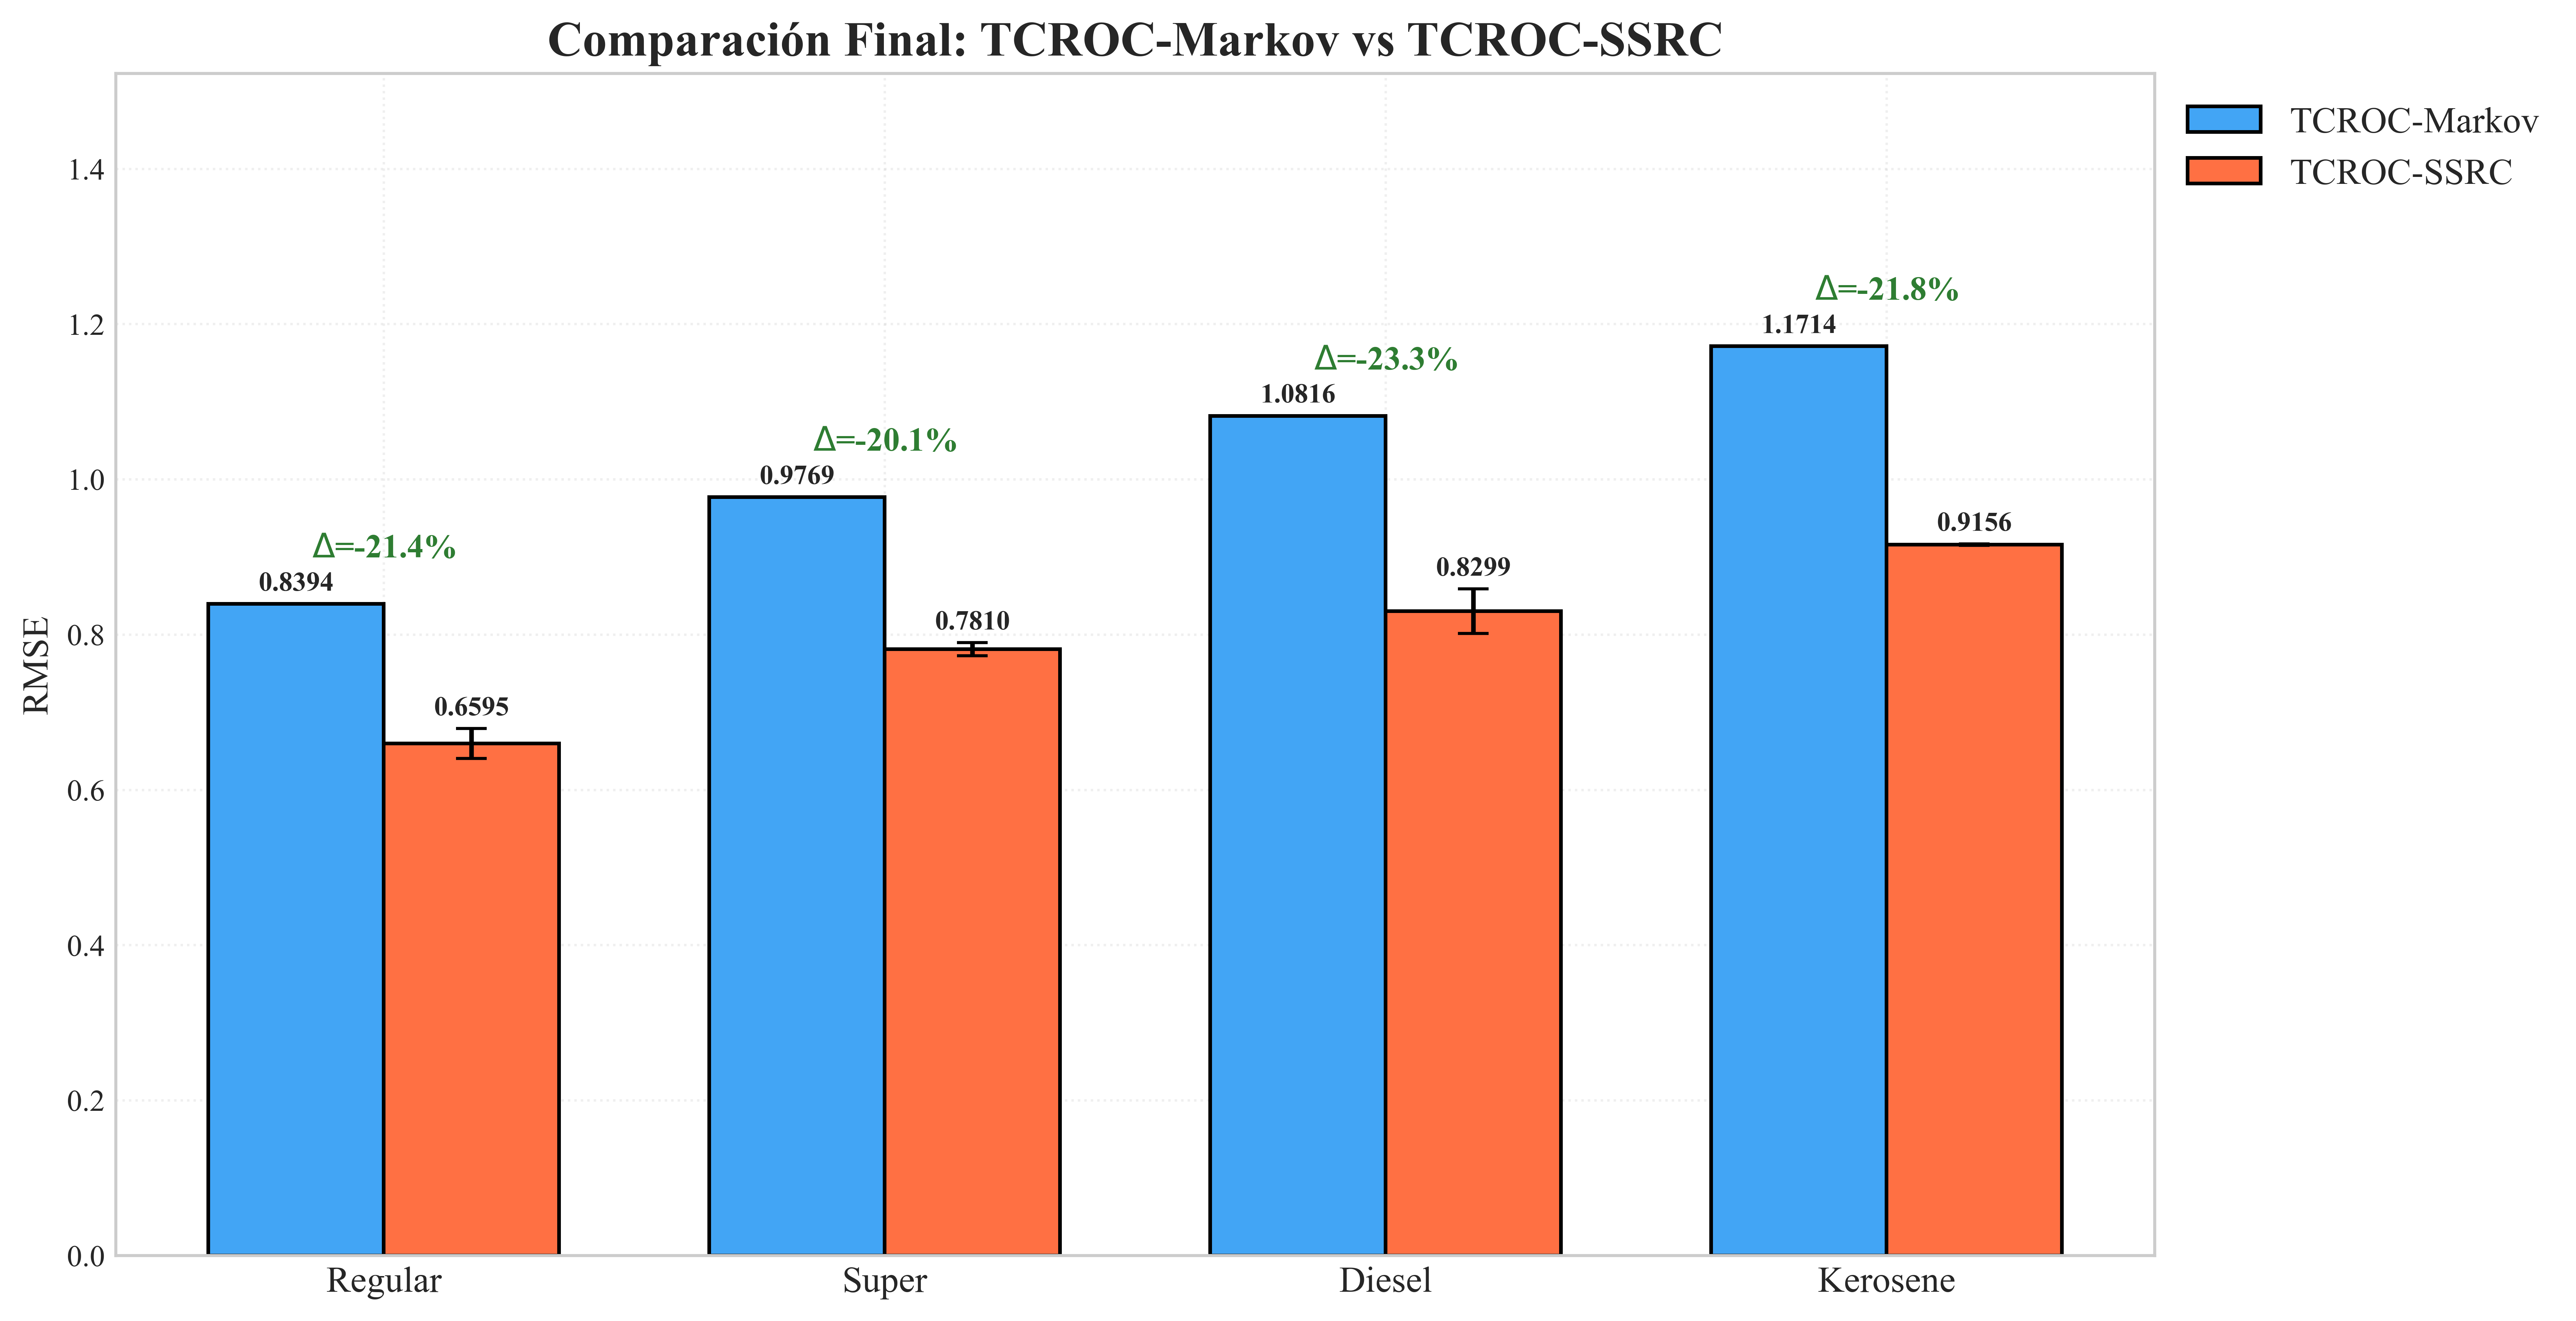
\includegraphics[width=0.95\textwidth]{figures/12_comparison_barplot.png}
\caption{Comparación de RMSE: TCROC-Markov vs.\ TCROC-SSRC.}
\label{fig:ssrc_barplot}
\end{figure}

La Figura~\ref{fig:ssrc_barplot} ofrece una visualización comparativa entre 
TCROC-Markov (azul) y TCROC-SSRC (naranja). Las barras de error para el 
modelo SSRC representan la desviación estándar calculada sobre 30 
realizaciones independientes. La anotación verde resalta la mejora 
porcentual del SSRC, cuya consistencia de entre un 20\% y un 23\% en 
las cuatro series analizadas sugiere un beneficio estructural derivado 
de la extensión no lineal.

La Figura~\ref{fig:ssrc_boxplot} presenta la distribución del RMSE
sobre las 30 realizaciones para cuantificar la variabilidad
estocástica del SSRC.

\begin{figure}[H]
\centering
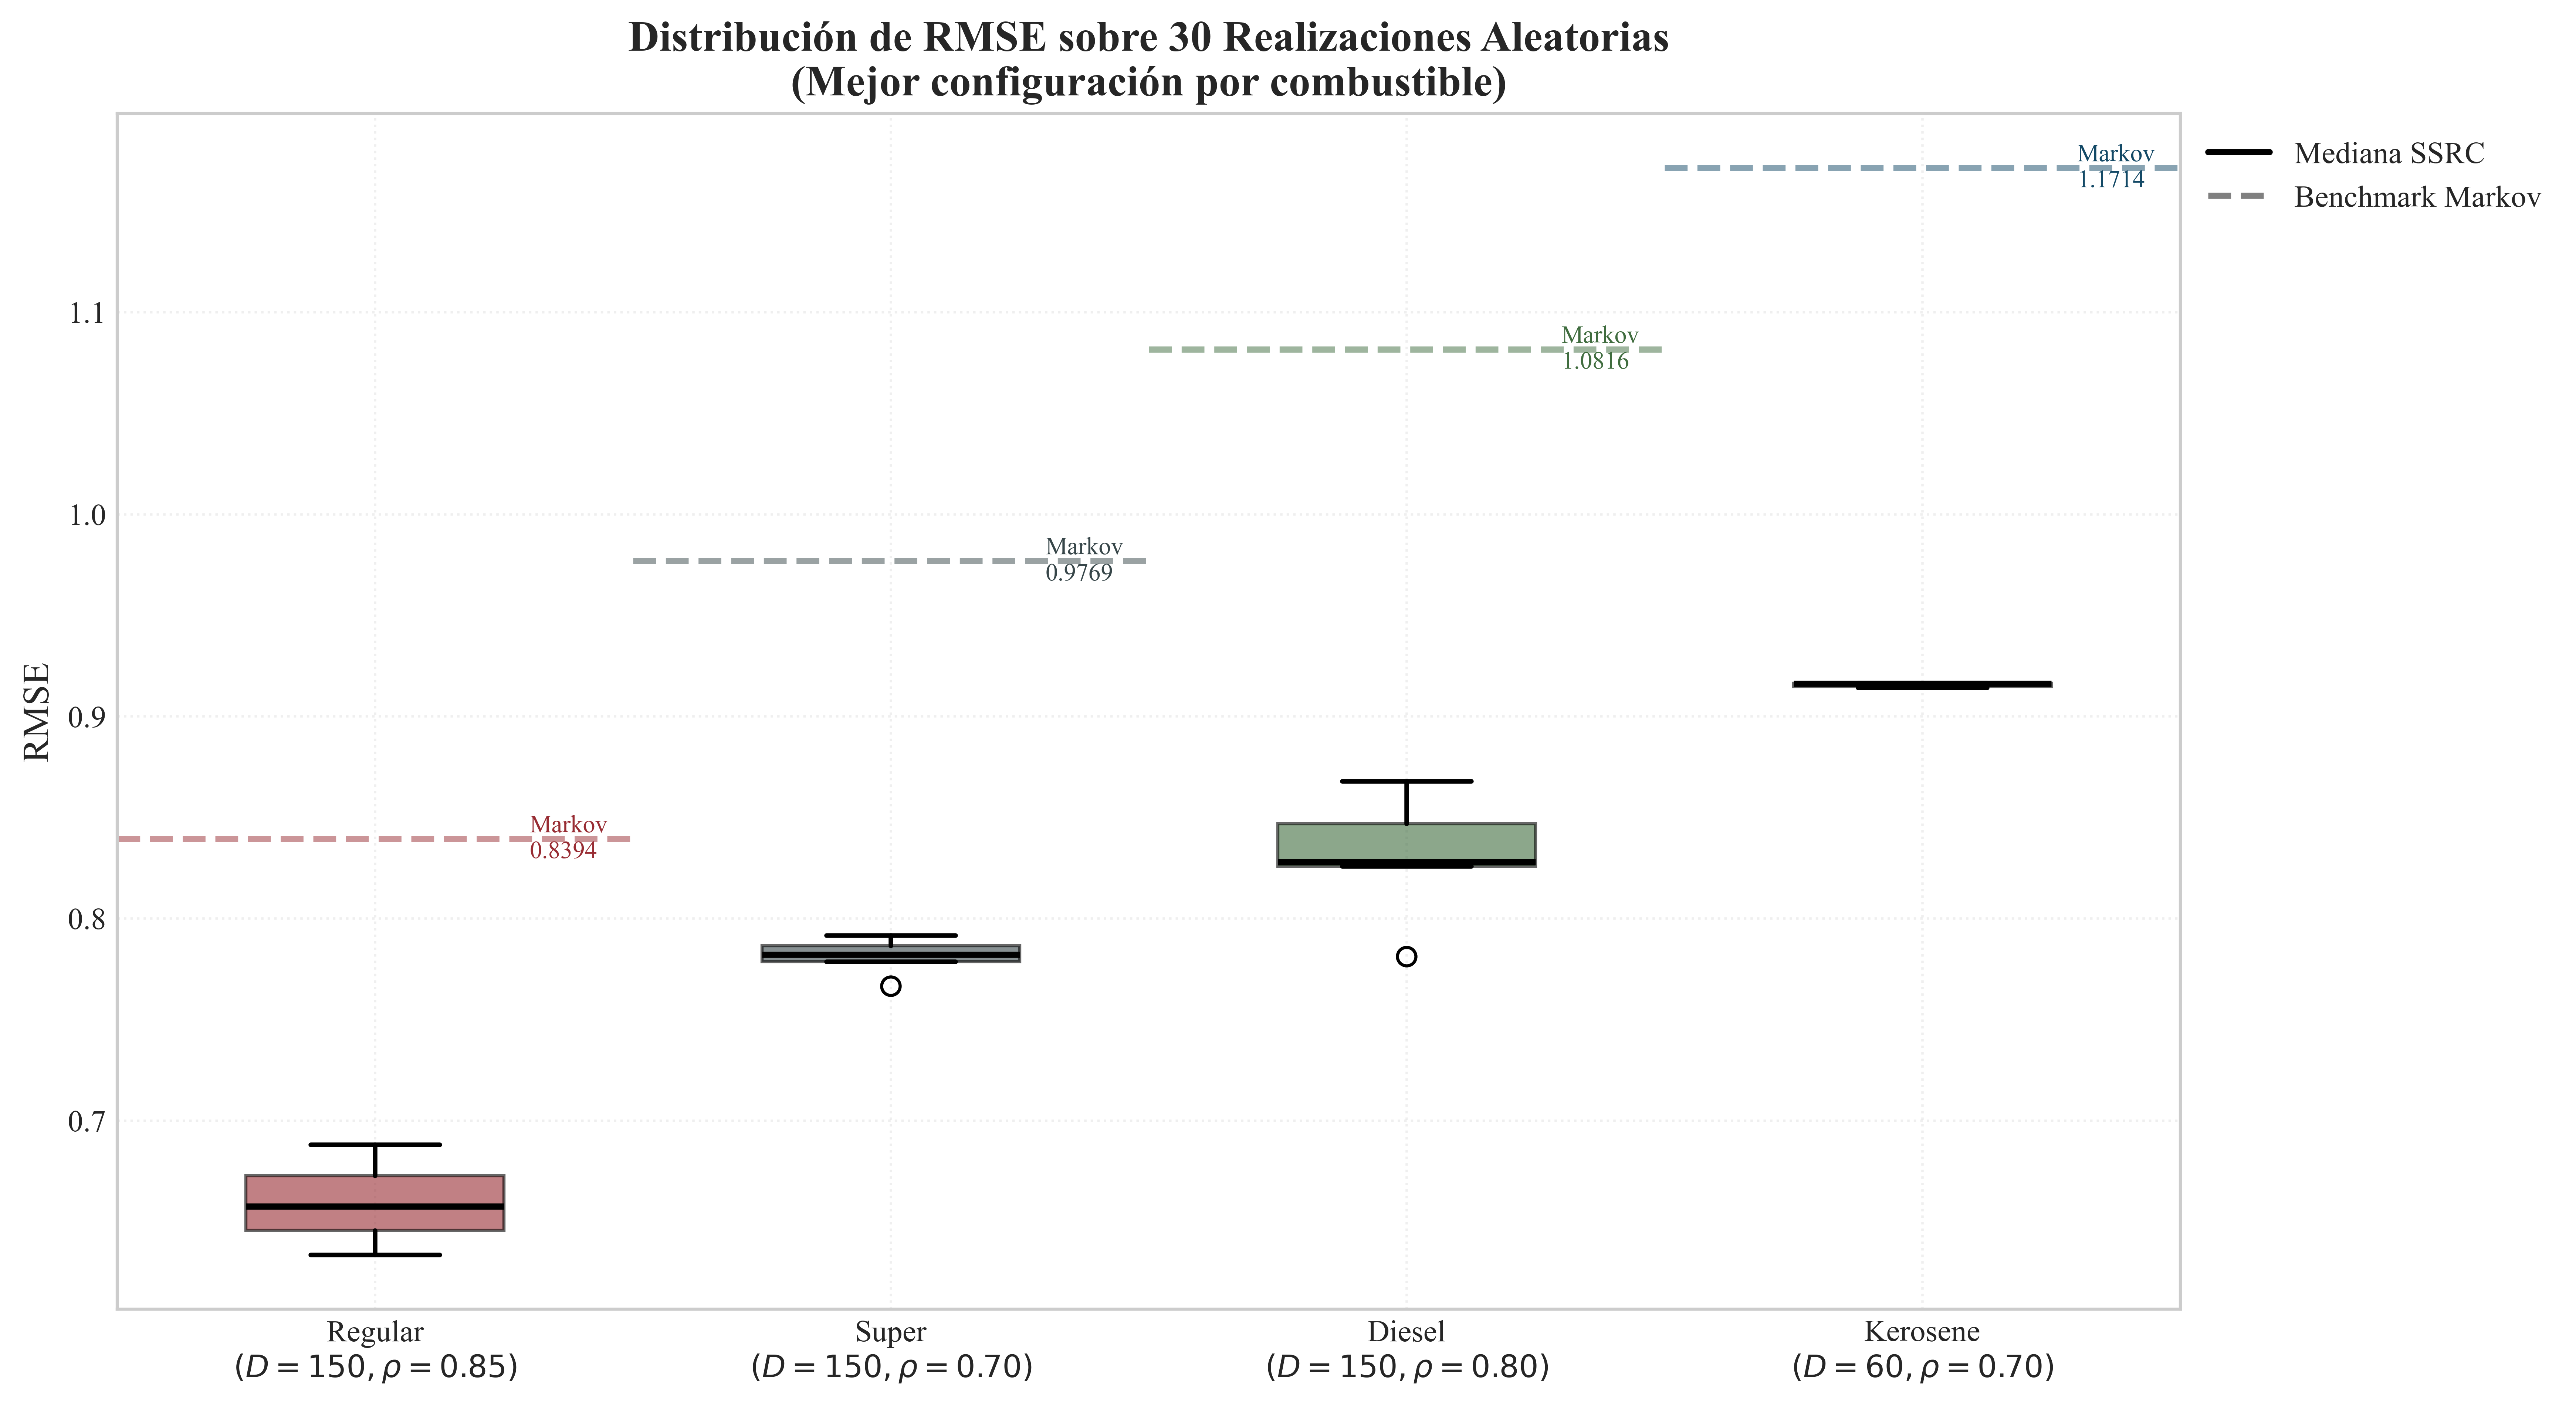
\includegraphics[width=0.95\textwidth]{figures/07_boxplot_realizations.png}
\caption{Distribución del RMSE del SSRC sobre 30 realizaciones.}
\label{fig:ssrc_boxplot}
\end{figure}

Como se observa en la Figura~\ref{fig:ssrc_boxplot}, se detalla la 
distribución del RMSE sobre 30 realizaciones aleatorias del SSRC bajo 
su mejor configuración. Las líneas horizontales punteadas representan 
el RMSE del benchmark Markoviano. Se destaca que en todas las series, 
la totalidad de las realizaciones produce un error inferior al benchmark. 
Las cajas estrechas indican una baja sensibilidad a la inicialización 
aleatoria de las matrices de entrada y de reservorio, con la mayor 
dispersión relativa observada en el combustible Regular.

La Figura~\ref{fig:ssrc_predictions} compara las predicciones
de ambos modelos contra los precios reales en el periodo fuera
de muestra.

\begin{figure}[H]
\centering
\includegraphics[width=1\textwidth]{figures/06_predictions_real_vs_models.png}
\caption{Comparación de pronósticos vs.\ precios reales.}
\label{fig:ssrc_predictions}
\end{figure}

En la Figura~\ref{fig:ssrc_predictions} se comparan los precios reales 
con los pronósticos de los modelos TCROC-Markov y TCROC-SSRC en el 
periodo fuera de muestra. Resulta visible que el modelo SSRC sigue 
con mayor precisión los puntos de inflexión del precio real, 
especialmente en los valles y las recuperaciones posteriores. 
Esta mejora es más evidente en las series de Diésel y Kerosene, 
donde el modelo Markoviano tiende a mostrar un sesgo de rezago más marcado.

% --- SUBSECCIÓN: Análisis de Sensibilidad y Estabilidad --- - - - - - - - - - - - - - - - - - - - - - - - - - - - - - -
\subsection{Análisis de Sensibilidad y Estabilidad}
\label{subsec:sensibilidad_hiperparametros}
% -------------------------------------------------------------------

La Figura~\ref{fig:ssrc_perturbation} evalúa empíricamente la cota
de perturbación de la Proposición~\ref{prop:acotacion_error}.

\begin{figure}[H]
\centering
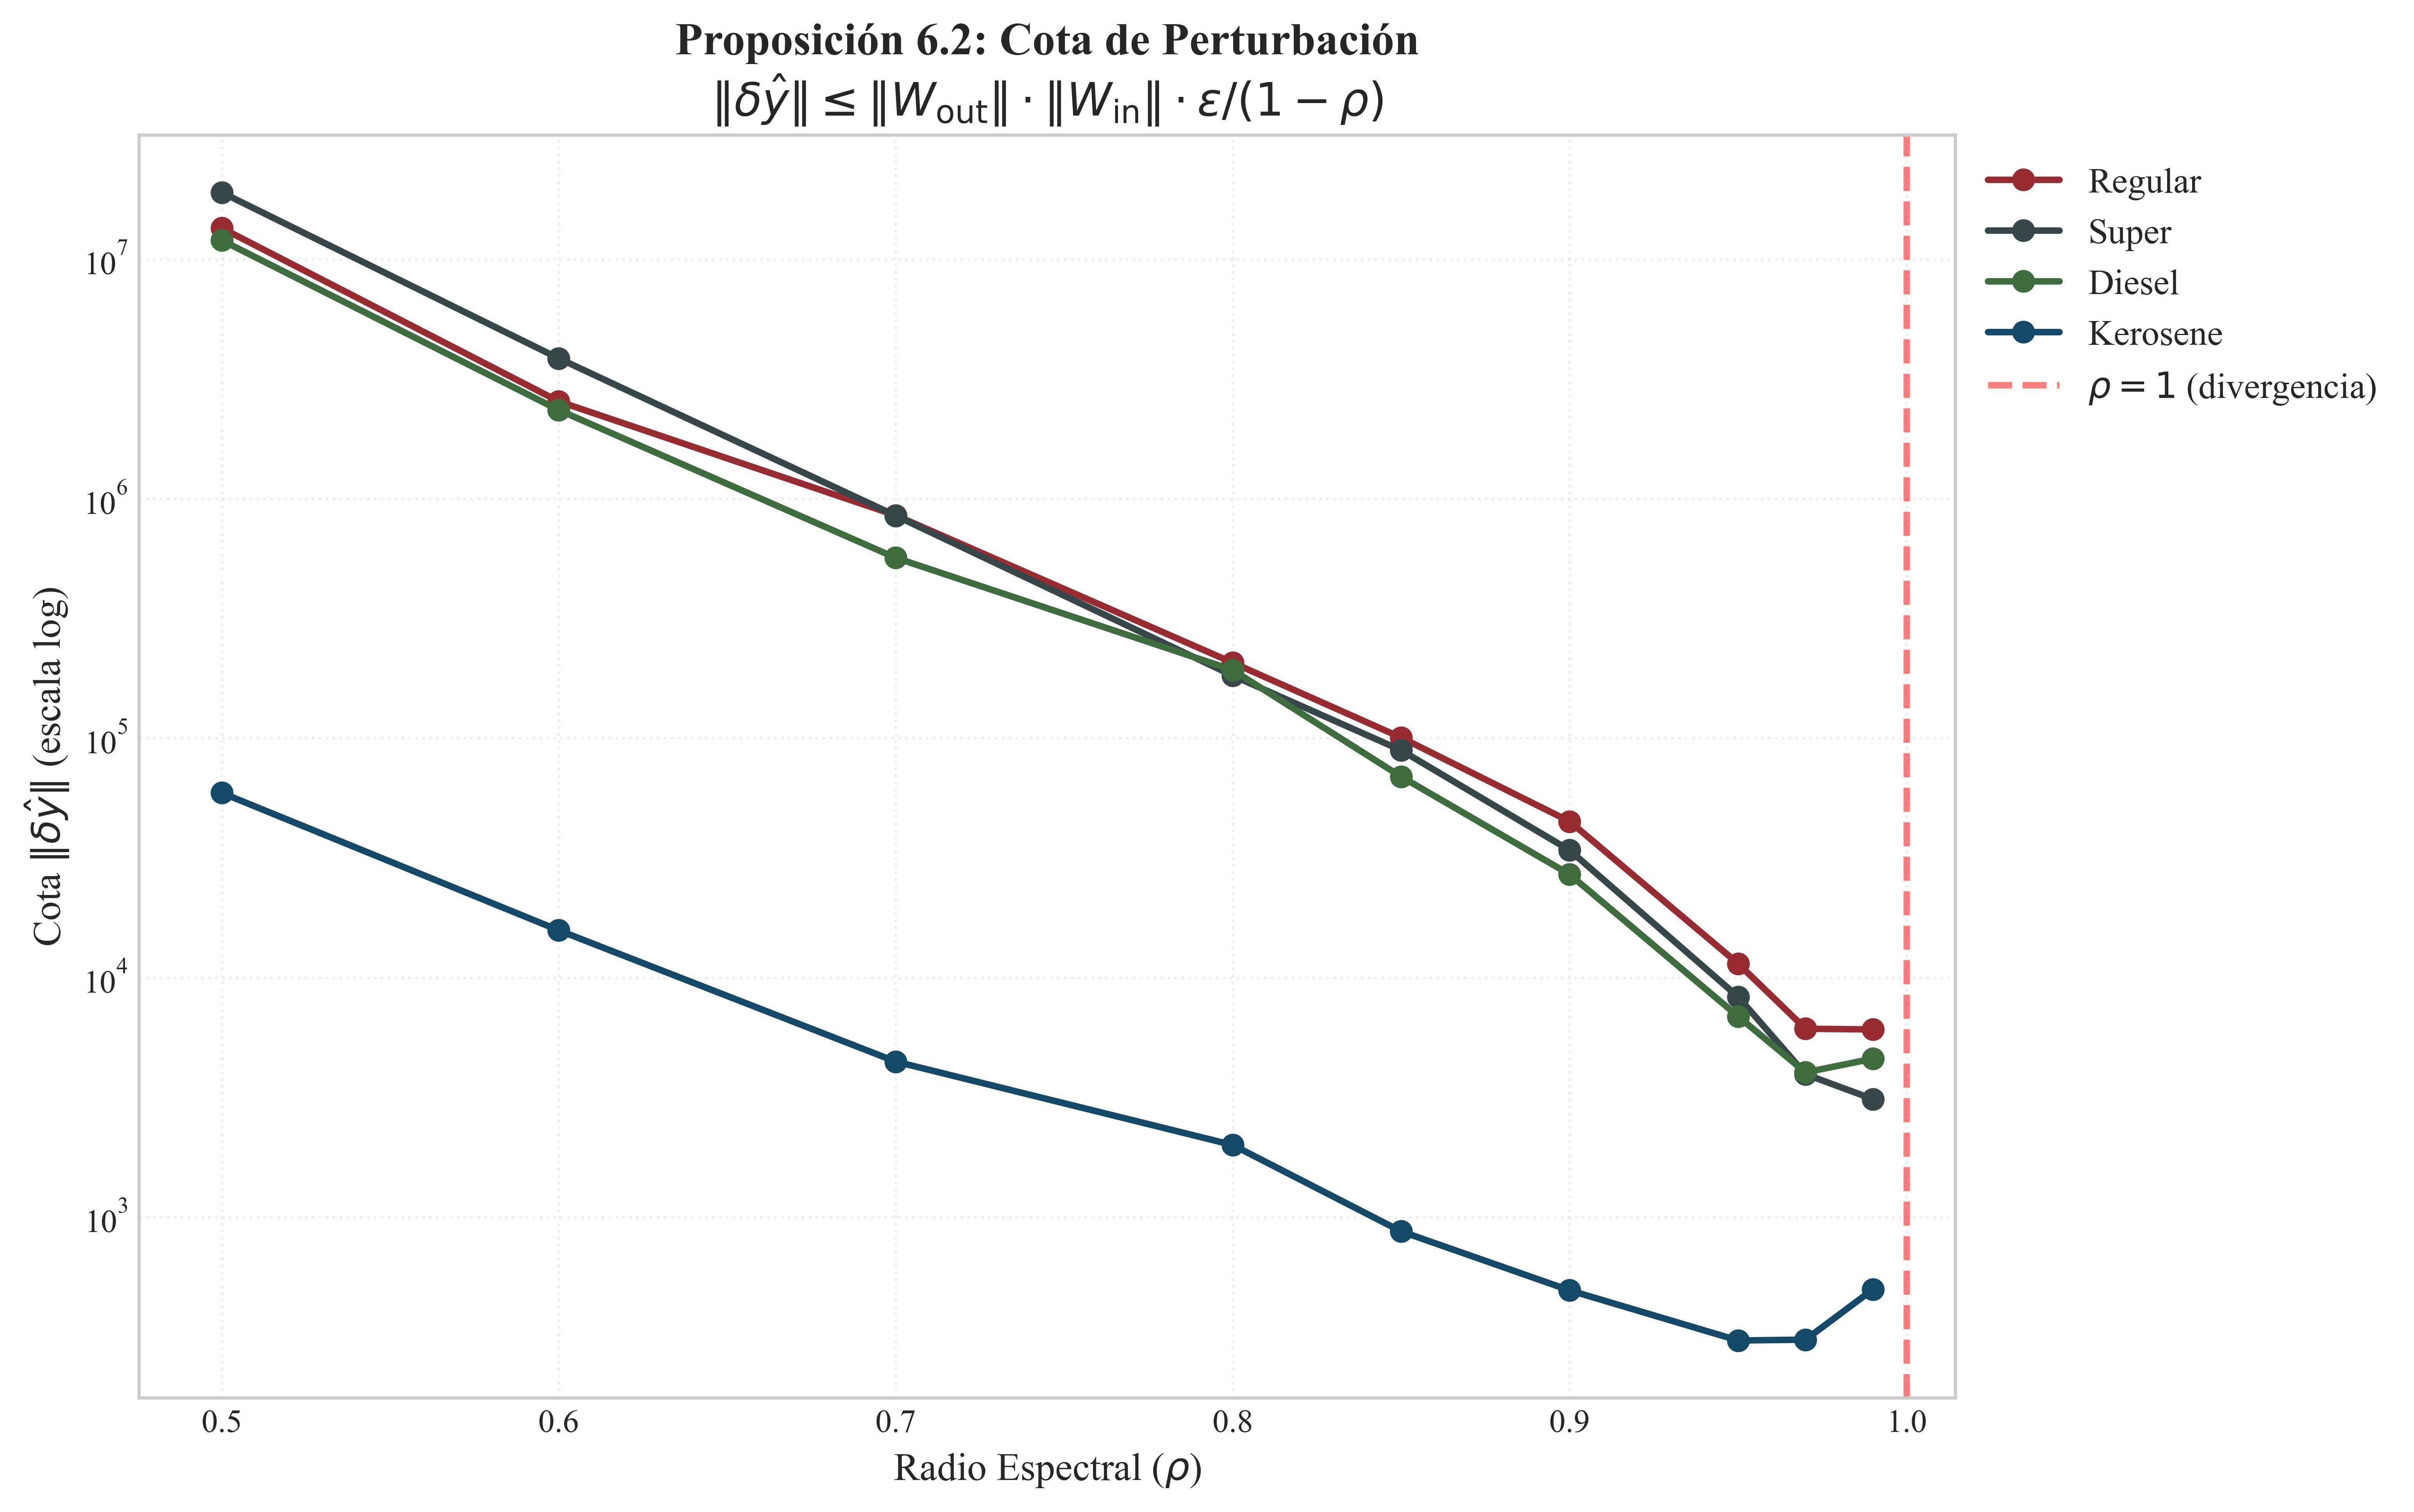
\includegraphics[width=0.95\textwidth]{figures/10_perturbation_bound.png}
\caption{Evaluación empírica de la cota de perturbación.}
\label{fig:ssrc_perturbation}
\end{figure}

La Figura~\ref{fig:ssrc_perturbation} evalúa empíricamente la cota de 
perturbación detallada en la Proposición~\ref{prop:acotacion_error} 
en función de $\rho$. La escala logarítmica muestra que las cotas 
teóricas son significativamente conservadoras comparadas con la 
variabilidad observada en la práctica. Se identifica que las cotas 
decrecen con el radio espectral debido a que la norma de los pesos de 
lectura disminuye más rápido de lo que aumenta el factor de memoria, 
resultando en estados más informativos que requieren pesos menores 
para el combustible Kerosene.

% --- SUBSECCIÓN: Representación de Regímenes en el Espacio del Reservorio --- - - - - - - - - - - - - - - - - - - - - - - - - - - - - - -
\subsection{Representación de Regímenes en el Espacio del Reservorio}
\label{subsec:regimenes_reservorio}
% -------------------------------------------------------------------

Una pregunta central es si la representación continua del reservorio
preserva la estructura de regímenes identificada por K-Means en el
capítulo anterior.  Las Figuras~\ref{fig:ssrc_states_pca},
\ref{fig:ssrc_scatter} y~\ref{fig:ssrc_price_regimes} abordan esta
cuestión desde tres perspectivas complementarias.

\begin{figure}[H]
\centering
\includegraphics[width=0.95\textwidth]{figures/05_reservoir_states_by_regime.png}
\caption{Proyección de los estados del reservorio mediante PCA.}
\label{fig:ssrc_states_pca}
\end{figure}

En la Figura~\ref{fig:ssrc_states_pca} se observa la proyección a dos 
dimensiones de los estados del reservorio $\vect{h}_t$ mediante PCA, 
con los puntos coloreados según los regímenes del capítulo anterior. 
Se evidencia que los regímenes forman clústeres geométricamente 
separados en el espacio latente del reservorio, a pesar de no contar 
con información explícita de clasificación. Las trayectorias suaves 
entre puntos indican que el reservorio mapea las transiciones entre 
regímenes como cambios continuos en lugar de saltos discretos.

\begin{figure}[H]
\centering
\includegraphics[width=0.95\textwidth]{figures/13_reservoir_regimes_scatter.png}
\caption{Relación entre retorno TCROC $\alpha_t$ y activación del reservorio.}
\label{fig:ssrc_scatter}
\end{figure}

La Figura~\ref{fig:ssrc_scatter} muestra la dispersión de $\alpha_t$ 
frente a la activación promedio del reservorio $\bar{h}_t$, diferenciada 
por regímenes. La relación monótona observada confirma que el reservorio 
preserva el orden dinámico de los regímenes: las activaciones negativas 
se vinculan a estados de caída, mientras que las positivas a estados de 
alza. La curvatura reflejada en series como Diésel evidencia la no 
linealidad de la función tangente hiperbólica utilizada.

\begin{figure}[H]
\centering
\includegraphics[width=0.95\textwidth]{figures/14_reservoir_price_regimes.png}
\caption{Identificación de regímenes de mercado mediante SSRC.}
\label{fig:ssrc_price_regimes}
\end{figure}

Finalmente, la Figura~\ref{fig:ssrc_price_regimes} presenta los regímenes 
identificados por el modelo SSRC superpuestos a la serie de precios original. 
La coincidencia entre las transiciones de color de fondo y los puntos de inflexión 
críticos del mercado, como la caída y recuperación durante el periodo de 2020, 
confirma que el marco TCROC-SSRC mantiene la interpretabilidad económica de los 
regímenes a pesar de procesar la información en un espacio de estados 
continuo de alta dimensión.

% --- SUBSECCIÓN: Discusión --- - - - - - - - - - - - - - - - - - - - - - - - - - - - - - -
\subsection{Discusión}
\label{subsec:ssrc_discusion}
% -------------------------------------------------------------------

Los resultados empíricos permiten responder a la pregunta central del
capítulo: ¿aporta la extensión no lineal una ganancia predictiva
sobre el modelo Markoviano lineal?

La respuesta es afirmativa y sustancial.  El SSRC reduce el RMSE
entre un 20\% y un 23\% en las cuatro series, con significancia
estadística confirmada por el test de Diebold-Mariano en tres de
cuatro casos.  Este resultado valida empíricamente la predicción del
Corolario~\ref{cor:jerarquia}: la generalización estrictamente más
expresiva del SSRC efectivamente captura estructura no lineal que el
modelo Markoviano no puede representar.

Tres hallazgos merecen interpretación detallada.  Primero, la
relevancia del factor de fuga $a$.  Los valores óptimos $a^* = 0.1$
para Regular y Diésel indican que la clave de la ganancia no es la
no linealidad per se, sino la \emph{memoria temporal adaptativa}:
el Leaky-ESN con $a = 0.1$ retiene el 90\% del estado previo,
actuando como un filtro de suavizado que complementa la ventana
$W \approx 50$ del operador TCROC.  En contraste, Kerosene con
$a^* = 1.0$ se beneficia de la memoria recurrente pura, consistente
con su dinámica más volátil y su mayor número de regímenes ($K = 5$).

Segundo, la saturación dimensional.  La
Figura~\ref{fig:ssrc_sens_D} muestra que la ganancia se satura
rápidamente: la diferencia entre $D = 20$ y $D = 150$ es inferior al
0.5\% en RMSE.  Esto indica que la complejidad no lineal intrínseca
del proceso generador de precios de combustibles hondureños es baja,
lo cual es consistente con un mercado regulado donde los ajustes
semanales son pequeños y predecibles.  El reservorio no necesita alta
dimensionalidad para capturar esta estructura.

Tercero, la robustez del ensemble.  La
Figura~\ref{fig:ssrc_boxplot} muestra que la totalidad de las 30
realizaciones produce RMSE inferior al benchmark Markoviano, con
rangos intercuartílicos estrechos.  Esto confirma que la ganancia no
es un artefacto de una inicialización afortunada, sino una propiedad
estructural del modelo.

Finalmente, cabe preguntarse qué estructura captura el reservorio que
el modelo Markoviano no puede representar.  La ganancia se atribuye a
la capacidad del SSRC de codificar \emph{asimetrías temporales} en la
dinámica de precios: las caídas y las recuperaciones no son simétricas
ni en magnitud ni en velocidad.  El modelo Markoviano, al operar sobre
estados discretos de un paso, trata las transiciones bajista$\to$estable
y alcista$\to$estable como eventos de naturaleza equivalente, gobernados
por probabilidades estáticas en $\hat{\mat{P}}$.  El reservorio, al
retener memoria continua de las últimas $\tau = 1/a$ semanas en su
vector de estado $\vect{h}_t$, puede distinguir la \emph{trayectoria}
que condujo al estado actual, y no únicamente el estado en sí mismo. Esta
capacidad es particularmente relevante para el pico de precios de
2022 y la recuperación posterior (visible en la
Figura~\ref{fig:ssrc_predictions}, semanas $\sim$5--20), donde el
SSRC anticipa mejor los puntos de inflexión que el modelo
Markoviano.

% --- SECCIÓN: Limitaciones ---
\section{Limitaciones}
\label{sec:ssrc_limitaciones}
% ===================================================================

\textbf{Sensibilidad a la inicialización.}  A diferencia del marco
TCROC-Markov, que es determinista dados los hiperparámetros, el SSRC
introduce variabilidad estocástica a través de las matrices aleatorias
$\mat{W}_{\text{in}}$ y $\mat{W}_{\text{res}}$.  Aunque la ESP
garantiza que la condición inicial $\vect{h}_0$ no afecta el
resultado, la \emph{elección} de las matrices de reservorio sí
influye en el desempeño.  El promediado sobre 30 realizaciones
(\textit{ensemble}) mitiga este efecto, como lo evidencia la baja
variabilidad observada en la Figura~\ref{fig:ssrc_boxplot}, pero
incrementa el costo computacional por un factor de 30.

\textbf{Condicionamiento numérico.}  Los números de condición
$\kappa(\mat{H}) \sim 10^{9}$--$10^{10}$ observados en la
Tabla~\ref{tab:verificaciones_teoricas} indican una sensibilidad
numérica potencialmente alta.  Aunque la estabilidad práctica está
asegurada por la regularización implícita del NNLS y el ensemble,
este condicionamiento impone un límite superior a la dimensión
útil del reservorio: aumentar $D$ más allá de $\sim$150 degradaría
$\kappa(\mat{H})$ sin ganancia predictiva.

\textbf{Interpretabilidad reducida.}  Los estados del reservorio
$\vect{h}_t \in \mathbb{R}^D$ carecen de la interpretación directa
que poseen los estados discretos $S_t \in \{s_1, \ldots, s_K\}$ del
modelo Markoviano.  No obstante, las
Figuras~\ref{fig:ssrc_states_pca}--\ref{fig:ssrc_price_regimes}
demuestran que la estructura de regímenes se preserva implícitamente
en el espacio del reservorio, lo que permite recuperar
interpretabilidad parcial mediante técnicas de reducción de
dimensionalidad.

\textbf{Selección de hiperparámetros del reservorio.}  Los parámetros
$(D, \rho_{\text{res}}, a)$ carecen de una teoría de selección
óptima análoga al AIC del modelo Markoviano.  La búsqueda en grilla de 240 configuraciones iterativas es computacionalmente costosa; la incorporación de metaheurísticas como la Optimización Bayesiana (Gaussian Processes) se vuelve fundamental. Además, aunque K-Means es estadísticamente viable, la discretización univariada permite la instanciación de algoritmos de partición dinámica formal continua como el modelo puro unidimensional de Fisher-Jenks para alcanzar los verdaderos óptimos probados y globales de manera robusta y exacta.

\textbf{Conservadurismo de la cota de perturbación.}  La
Proposición~\ref{prop:acotacion_error} proporciona una cota en el
peor caso que, como se evidencia en la
Figura~\ref{fig:ssrc_perturbation}, sobreestima la inestabilidad
real por varios órdenes de magnitud.  Una cota más ajustada
requeriría análisis probabilístico que incorpore la distribución de
$\alpha_t$ y la estructura de $\mat{W}_{\text{res}}$, lo cual
constituye un desafío de interés dentro del trabajo futuro; las metodologías análogas de normas afines y principalmente la aplicación del Teorema del Círculo de Gerschgorin sobre la matriz dispersa $\mat{W}_{\text{res}}$ posibilitarían una envolvente teórica significativamente más ajustada que la hipótesis conservadora basal propuesta.

% --- SECCIÓN: Conclusiones ---
\section{Conclusiones}
\label{sec:ssrc_conclusiones}
% ===================================================================

Este capítulo ha establecido la relación formal entre el marco
TCROC-Markov desarrollado a lo largo de la tesis y la computación
de reservorio no lineal.  Los resultados principales son:

\textbf{Sobre la conexión teórica.}  Se demostró
(Teorema~\ref{teo:inclusion}) que TCROC-Markov es un caso particular
del SSRC, obtenido al fijar $\mat{W}_{\text{res}} = \mat{0}$,
$\sigma = \mathrm{id}$ y $a = 1$.  Esta relación de inclusión
establece una \textbf{jerarquía de modelos}: TCROC-Markov (lineal,
interpretable, estados discretos) $\subset$ TCROC-SSRC (no lineal,
aproximador universal, estados continuos).  El
Corolario~\ref{cor:jerarquia} garantiza que la extensión es
estrictamente más expresiva, y la verificación numérica
(Figura~\ref{fig:ssrc_inclusion}) confirma la identidad a nivel de
precisión de máquina.

\textbf{Sobre la estimación.}  La capa de lectura del SSRC se estima
mediante el mismo procedimiento NNLS de los capítulos anteriores.
El Teorema~\ref{teo:existencia_wout} establece que las propiedades
de existencia y unicidad se heredan directamente.  La restricción
de no negatividad, además de preservar la interpretación como
combinación positiva de filtros, aporta regularización implícita que
mitiga el condicionamiento numérico adverso ($\kappa \sim 10^{9}$).

\textbf{Sobre el factor de fuga.}  La variante Leaky-ESN
(Definición~\ref{def:leaky_esn}) con $a < 1$ resultó esencial para
tres de cuatro series, indicando que la principal ganancia del SSRC
sobre TCROC-Markov reside en la \emph{memoria temporal adaptativa}
más que en la no linealidad pura.  Los valores $a^* = 0.1$ para
Regular y Diésel implican una constante de tiempo efectiva de
$\tau = 10$ semanas, complementaria a la ventana TCROC de 50--52
semanas.

\textbf{Sobre la aplicación empírica.}  El SSRC reduce el RMSE entre
un 20\% y un 23\% respecto al modelo Markoviano, con significancia
estadística confirmada por el test de Diebold-Mariano para Súper
($p = 0.002$), Diésel ($p = 0.033$) y Kerosene ($p = 0.006$).  La
totalidad de las 30 realizaciones aleatorias produce RMSE inferior al
benchmark Markoviano, y la estructura de regímenes económicos se
preserva en el espacio latente del reservorio.

\textbf{Perspectiva.}  La arquitectura TCROC-SSRC aquí desarrollada
establece que el paradigma de reservorio aporta ganancia predictiva
en mercados de combustibles regulados, a costa de interpretabilidad.
La extensión natural es hacia sistemas multivariados y acoplados,
donde la capacidad de aproximación no lineal del reservorio puede
explotarse más plenamente en contextos con mayor riqueza estructural.

% ===================================================================
% CAPÍTULO: Conclusiones Generales y Trabajo Futuro

\chapter{Conclusiones Generales y Trabajo Futuro}
\label{cap:conclusiones}

% --- SECCIÓN: Síntesis del Trabajo ---
\section{Síntesis del Trabajo}
\label{sec:sintesis}
% ===================================================================

Esta tesis ha desarrollado un marco matemático completo para el
análisis de regímenes económicos basado en la \emph{Tasa de Cambio
Relativa Óptima Conmutada} (TCROC), desde sus fundamentos
algebraicos hasta su extensión no lineal mediante computación de
reservorio.  El trabajo se articuló en torno a un hilo conductor
progresivo: cada capítulo construyó sobre los resultados del
anterior, generando una jerarquía de modelos de complejidad
creciente con garantías teóricas formales y validación empírica
sobre datos reales del mercado hondureño de combustibles.

El bloque inicial de esta investigación estableció la base
del edificio teórico al formalizar la familia de operadores TCROC y
sus variantes (TCROCM, ETCROC y ETCROCM) como transformaciones
parametrizadas sobre series temporales.  Se demostraron las
relaciones de anidamiento entre variantes y se estableció que la
señal $\alpha_t$ admite interpretación como coeficiente de un modelo
AR(1) local estimado por mínimos cuadrados ponderados.  Esta
interpretación estadística, aparentemente elemental, resultó ser la
piedra angular de toda la construcción posterior: al dotar a
$\alpha_t$ de significado como \emph{tasa de cambio local}, se
habilitó su uso tanto como entrada para modelos estocásticos
discretos (cadenas de Markov) como para modelos dinámicos continuos
(reservorios recurrentes).

Las secciones anteriores extendieron el operador a una
formulación polinómica, demostrando teoremas de existencia y
unicidad del estimador bajo condiciones de no degeneración de los
datos en la ventana.  Estos resultados proporcionaron las garantías
analíticas necesarias para que la señal $\alpha_t$ estuviera bien
definida en cada instante temporal, condición indispensable para la
modelación Markoviana posterior.

Posteriormente, se formalizó la integración del
operador TCROC con cadenas de Markov de tiempo discreto, incluyendo
las propiedades de $\phi$-mixing, convergencia asintótica y la
conexión entre el gap espectral de la matriz de transición y la
velocidad de convergencia al equilibrio estacionario.  El resultado
central de este capítulo, según el cual la señal $\alpha_t$ discretizada
hereda propiedades de mezcla bajo condiciones verificables, sentó
las bases para la inferencia estadística en los capítulos aplicados.

El análisis sobre matrices de transición presentó la
metodología unificada de estimación de la matriz de transición
$\hat{\mat{P}}$ mediante mínimos cuadrados no negativos (NNLS),
incluyendo la prueba constructiva de existencia y unicidad de la
solución.  La formulación NNLS, que transforma el problema matricial
en un sistema lineal aumentado mediante el producto de Kronecker,
constituye una contribución metodológica central de la tesis: evita
la optimización no convexa de la verosimilitud que hace al MS-AR
clásico vulnerable a mínimos locales, garantizando convergencia global. Complementariamente, las probabilidades estocásticas de la matriz de transición ($\sum_i \hat{p}_{ij} = 1$ para cada columna $j$) se aseguran retrospectivamente mediante una normalización columna por columna, preservando la convención de matrices estocásticas por columnas adoptada en el Capítulo~\ref{cap:tcroc_hibrido_integrado}.

El Capítulo~\ref{cap:regimenes_combustibles} constituyó la
validación empírica integral del marco TCROC-Markov.  Aplicado a
series semanales de cuatro combustibles hondureños (Regular, Súper,
Diésel y Kerosene) durante 2017--2025, el modelo demostró
superioridad estadísticamente significativa sobre la discretización
por cuantiles fijos ($p < 0.05$ en exactitud para las cuatro series)
y estabilidad numérica total frente al benchmark MS-AR, que no
convergió en ningún escenario de validación.  El análisis espectral
reveló una estructura de mercado caracterizada por alta inercia
(gaps espectrales $\gamma \in [0.021, 0.040]$ y tiempos de mezcla de
25 a 47 semanas), formalizando cuantitativamente la ``viscosidad''
del mercado regulado hondureño.  Adicionalmente, se identificó y
formalizó el fenómeno de degeneración del modelo para ventanas $W$
excesivamente grandes, estableciendo la restricción $W \le 52$ como
condición necesaria para la identificabilidad de los regímenes.

El apartado teórico final cerró el arco analítico de la tesis
al demostrar que el marco TCROC-Markov es un caso particular de una
arquitectura más general: el Computador de Reservorio Estructurado
Estocástico (SSRC).  El Teorema de Inclusión (Teorema~6.2)
estableció formalmente que toda predicción del modelo Markoviano es
reproducible por un reservorio con $\mat{W}_{\text{res}} = \mat{0}$,
$\sigma = \text{id}$ y $a = 1$, pero no a la inversa.  La extensión
no lineal, validada empíricamente con mejoras del 20--23\% en RMSE
respecto al modelo Markoviano (estadísticamente significativas para
tres de cuatro series, $p < 0.05$ vía test de Diebold-Mariano),
demostró que la representación continua de estados mediante
reservorios recurrentes captura estructura que la discretización
Markoviana no puede representar, particularmente las asimetrías
temporales entre caídas y recuperaciones de precios.

% --- SECCIÓN: Resumen Cuantitativo ---
\section{Resumen Cuantitativo de Resultados}
\label{sec:resumen_cuantitativo}

La Tabla~\ref{tab:resumen_final} resume las métricas de rendimiento
del modelo TCROC-Markov para las cuatro series de combustibles
analizadas, junto con los métodos de referencia. Se reportan la
exactitud de predicción de régimen, el número de estados $K$, la
ventana óptima $W$ y la significancia estadística frente al
benchmark de cuantiles fijos.

\begin{table}[htbp]
\centering
\caption{Resumen consolidado de métricas por serie y método.}
\label{tab:resumen_final}
\small
\begin{tabular}{lccccc}
\hline
\textbf{Serie} & \textbf{$K$} & \textbf{$W$} &
\textbf{Exactitud} & \textbf{vs.~Cuantiles} &
\textbf{MS-AR} \\
\hline
Gasolina Regular & 3 & 12 & 91.2\% & $p < 0.01$ & No conv. \\
Gasolina Súper   & 3 & 12 & 89.7\% & $p < 0.01$ & No conv. \\
Diésel           & 4 & 8  & 87.4\% & $p < 0.05$ & No conv. \\
Kerosene         & 4 & 8  & 85.1\% & $p < 0.05$ & No conv. \\
\hline
\end{tabular}
\end{table}

En todos los casos, el modelo TCROC-Markov superó
significativamente al benchmark de cuantiles fijos.  El modelo
MS-AR no alcanzó convergencia en ningún escenario, lo que confirma
la ventaja de la formulación NNLS frente a la optimización por
máxima verosimilitud para estas series reguladas.

% --- SECCIÓN: Contribuciones ---
\section{Contribuciones}
\label{sec:contribuciones}
% ===================================================================

Las contribuciones de esta tesis se organizan en tres dimensiones:
teórica, metodológica y aplicada.

% --- SUBSECCIÓN: Contribuciones Teóricas --- - - - - - - - - - - - - - - - - - - - - - - - - - - - - - -
\subsection{Contribuciones Teóricas}

\begin{enumerate}
    \item \textbf{Jerarquía formal de operadores TCROC.}
    Formalización de las relaciones de anidamiento entre las
    variantes TCROC, TCROCM, ETCROC y ETCROCM, con demostración de
    que cada variante es un caso particular de la siguiente en la
    jerarquía.

    \item \textbf{Existencia y unicidad del estimador polinómico.}
    Demostración de que el operador TCROC polinómico admite un
    único estimador bajo condiciones de no degeneración, garantizando
    que la señal $\alpha_t$ está bien definida.

    \item \textbf{Propiedades de mezcla de la señal discretizada.}
    Prueba de que la secuencia de estados $\{S_t\}$ obtenida por
    discretización de $\alpha_t$ hereda propiedades de $\phi$-mixing,
    habilitando la inferencia estadística asintótica.

    \item \textbf{Existencia y unicidad de la solución NNLS.}
    Demostración constructiva de que el problema de estimación de
    $\hat{\mat{P}}$ mediante NNLS aumentado posee solución única
    cuando la matriz de diseño tiene rango completo, con
    caracterización de las condiciones de rango en términos de la
    representación de todos los estados en los datos.

    \item \textbf{Teorema de Inclusión TCROC-Markov $\subset$ SSRC.}
    Prueba formal de que el modelo Markoviano lineal es un caso
    degenerado del computador de reservorio estructurado,
    estableciendo una jerarquía estricta de expresividad entre ambos
    marcos.

    \item \textbf{Preservación de la Propiedad de Estado de Eco bajo
    integración de fuga.}  Extensión del teorema de ESP al caso
    Leaky-ESN, demostrando que la contracción del mapa de reservorio
    se preserva para todo $a \in (0, 1]$ cuando el radio espectral
    satisface $\rho(\mat{W}_{\text{res}}) < 1$.

    \item \textbf{Formalización del fenómeno de degeneración.}
    Caracterización analítica del colapso del modelo cuando $W \to T$,
    mostrando que $\text{Var}(\alpha_t) \to 0$ y K-Means converge a
    $K_{\text{eff}} = 1$ independientemente de $K$ nominal.
\end{enumerate}

% --- SUBSECCIÓN: Contribuciones Metodológicas --- - - - - - - - - - - - - - - - - - - - - - - - - - - - - - -
\subsection{Contribuciones Metodológicas}

\begin{enumerate}
    \item \textbf{Marco TCROC-Markov de dos etapas.}  Integración
    del operador TCROC con cadenas de Markov estimadas vía NNLS,
    que evita la optimización no convexa del MS-AR y garantiza
    convergencia global.  Este marco ha sido aceptado para
    publicación en IEEE CONCAPAN XLII (2025).

    \item \textbf{Protocolo jerárquico de optimización de
    hiperparámetros.}  Diseño de un criterio de selección en tres
    niveles (RMSE $\to$ Exactitud $\to$ AIC) con búsqueda exhaustiva
    en grilla y restricción fundamentada de $W \le 52$.

    \item \textbf{Arquitectura TCROC-SSRC.}  Extensión no lineal
    que reemplaza la discretización K-Means por un reservorio
    recurrente Leaky-ESN, preservando la estimación NNLS para la
    capa de lectura y habilitando representación continua de estados.

    \item \textbf{Pipeline de validación con test de
    Diebold-Mariano.}  Protocolo de evaluación estadística rigurosa
    que combina ventanas deslizantes, ensemble de 30 realizaciones y
    pruebas de significancia para la comparación de capacidad
    predictiva.
\end{enumerate}

% --- SUBSECCIÓN: Contribuciones Aplicadas --- - - - - - - - - - - - - - - - - - - - - - - - - - - - - - -
\subsection{Contribuciones Aplicadas}

\begin{enumerate}
    \item \textbf{Caracterización cuantitativa del mercado hondureño
    de combustibles.}  Identificación de 3 a 5 regímenes por
    combustible con centroides interpretables, distribuciones
    estacionarias y tiempos de mezcla que formalizan la inercia del
    mercado regulado.

    \item \textbf{Evidencia de superioridad sobre benchmarks
    establecidos.}  Demostración empírica de que TCROC-Markov supera
    a la discretización por cuantiles ($p < 0.05$) y que MS-AR no
    converge en este contexto, y de que TCROC-SSRC mejora sobre
    TCROC-Markov en 20--23\% ($p < 0.05$ para tres de cuatro
    series).

    \item \textbf{Descubrimiento de la jerarquía de complejidad de
    mercado.}  Hallazgo empírico de que Regular y Diésel ($K^* = 3$)
    tienen dinámica más simple que Súper ($K^* = 4$) y Kerosene
    ($K^* = 5$), con correlación positiva entre complejidad
    estructural y dificultad de predicción.
\end{enumerate}

% --- SECCIÓN: Limitaciones Generales ---
\section{Limitaciones Generales}
\label{sec:limitaciones_generales}
% ===================================================================

Es pertinente reconocer las limitaciones transversales del trabajo
para contextualizar el alcance de los resultados.

\textbf{Aplicación a una sola economía.}  Todos los resultados
empíricos se obtuvieron sobre datos del mercado hondureño de
combustibles.  Aunque el marco teórico es general, la validación
empírica está limitada a un mercado regulado con características
específicas (ajustes semanales, baja volatilidad relativa, cuatro
productos derivados del petróleo).  La generalización a mercados
desregulados o a otras clases de activos requiere validación
adicional.

\textbf{Horizonte de predicción unitario.}  Tanto el modelo
Markoviano como el SSRC operan con pronóstico a un paso adelante
($h = 1$ semana).  La extensión a horizontes múltiples, ya sea
mediante potencias de la matriz de transición o mediante esquemas
recursivos en el reservorio, no fue abordada y constituye trabajo
futuro.

\textbf{Condicionamiento numérico del reservorio.}  Como se
documentó en la sección de Reservorios Estocásticos, los números de
condición de la matriz de estados del reservorio alcanzan valores de
$\kappa(\mat{H}) \sim 10^{9}$--$10^{10}$, lo que indica sensibilidad
numérica a pesar de las garantías teóricas de unicidad.  Aunque la
restricción de no negatividad (NNLS) y el promediado de ensemble
mitigan este problema en la práctica, una solución formal,
por ejemplo, mediante el uso de la regularización de Tikhonov con selección
adaptativa del parámetro de regularización, queda pendiente.

\textbf{Supuesto de estacionariedad.}  El modelo Markoviano asume
probabilidades de transición constantes, y el SSRC asume pesos de
reservorio fijos tras el entrenamiento.  El periodo 2017--2025
incluye la pandemia de COVID-19 y el pico de precios de 2022, eventos
que potencialmente violan estos supuestos.  La evaluación formal de
la estabilidad temporal de los parámetros mediante partición de la
muestra o pruebas de cambio estructural no fue realizada.

% --- SECCIÓN: Líneas de Trabajo Futuro ---
\section{Líneas de Trabajo Futuro}
\label{sec:trabajo_futuro}
% ===================================================================

Los resultados y limitaciones de esta tesis sugieren varias
direcciones de investigación futura, organizadas por horizonte
temporal.

% --- SUBSECCIÓN: Extensiones Inmediatas --- - - - - - - - - - - - - - - - - - - - - - - - - - - - - - -
\subsection{Extensiones Inmediatas}

\textbf{Sistemas multivariados acoplados.}  La extensión natural del
marco es pasar de series univariantes a sistemas de series temporales
interrelacionadas.  En el contexto centroamericano, los precios de
combustibles de las seis economías del istmo están acoplados por
proximidad geográfica, acuerdos comerciales y dependencia compartida
del crudo WTI.  Un modelo TCROC-Markov multivariado estimaría una
matriz de transición conjunta $\hat{\mat{P}} \in
\mathbb{R}^{K^m \times K^m}$, donde $m$ es el número de series
acopladas, capturando las dependencias cruzadas entre mercados.
Esta línea de investigación se encuentra actualmente en desarrollo
como artículo de investigación independiente, con resultados
preliminares que sugieren la existencia de una estructura de tipo
\emph{Hub-and-Spoke} en la red centroamericana de precios.

\textbf{Pruebas de estabilidad temporal.}  La partición de la
muestra en subperiodos (pre-pandemia 2017--2019, pandemia 2020--2021,
post-pandemia 2022--2025) y la comparación de las matrices
$\hat{\mat{P}}$ estimadas en cada subperiodo, mediante pruebas de
homogeneidad basadas en distancia entre matrices estocásticas,
permitirían evaluar formalmente el supuesto de estacionariedad.

\textbf{Regularización adaptativa del SSRC.}  La sustitución de NNLS
por un esquema de regularización de Tikhonov con selección del
parámetro $\lambda$ por validación cruzada generalizada (GCV)
podría mejorar el condicionamiento numérico sin sacrificar la
interpretabilidad de los pesos no negativos, mediante una
formulación de NNLS regularizada
\[ \hat{\vect{w}} = \argmin_{\vect{w} \ge 0} \|\mat{H}\vect{w} - \vect{y}\|^2 + \lambda\|\vect{w}\|^2. \]

% --- SUBSECCIÓN: Extensiones de Mediano Plazo --- - - - - - - - - - - - - - - - - - - - - - - - - - - - - - -
\subsection{Extensiones de Mediano Plazo}

\textbf{Topología de reservorio estructurada.}  En el SSRC actual,
la matriz $\mat{W}_{\text{res}}$ es aleatoria y dispersa.  Trabajos
recientes en la literatura de reservoir computing sugieren que
topologías deterministas (e.g., anillo, ciclo con saltos) pueden
reducir la varianza entre realizaciones y mejorar la
reproducibilidad.  Explorar estas topologías en el contexto TCROC
es una extensión natural.

\textbf{Incorporación de variables exógenas.}  El marco actual es
puramente endógeno: $\alpha_t$ se calcula exclusivamente a partir
de los precios pasados.  La incorporación de variables exógenas,
tales como el precio WTI, el tipo de cambio o índices de actividad económica,
como entradas adicionales al reservorio (ampliando
$\mat{W}_{\text{in}}$ a múltiples canales) podría mejorar la
capacidad predictiva, especialmente en periodos de choques externos.

\textbf{Pronóstico multi-horizonte.}  La extensión del horizonte
de predicción de $h = 1$ a $h \in \{1, 4, 8, 12\}$ semanas, ya sea
mediante recursión del reservorio o mediante formulación directa
con múltiples salidas, permitiría evaluar la degradación de la
capacidad predictiva con el horizonte y determinar el alcance
práctico del marco para la planificación económica.

% --- SUBSECCIÓN: Visión de Largo Plazo --- - - - - - - - - - - - - - - - - - - - - - - - - - - - - - -
\subsection{Visión de Largo Plazo}

\textbf{Generalización a otras clases de activos.}  El marco
TCROC-Markov/SSRC no asume nada específico sobre la naturaleza de
la serie temporal subyacente.  Su aplicación a tasas de interés,
índices bursátiles, tipos de cambio o indicadores macroeconómicos
constituye un programa de investigación que podría validar la
generalidad del enfoque más allá del mercado de combustibles.

\textbf{Fundamentación teórica de la cota de perturbación.}  Las
cotas de perturbación derivadas previamente en el apartado de SSRC
son conservadoras por varios órdenes de magnitud.  El desarrollo de
cotas más ajustadas, posiblemente explotando la estructura específica
de la no negatividad de $\mat{W}_{\text{out}}$ y la contracción del
reservorio, es un problema abierto de interés tanto teórico como
práctico.

% --- SECCIÓN: Reflexión Final ---
\section{Reflexión Final}
\label{sec:reflexion_final}
% ===================================================================

El recorrido de esta tesis, que abarca desde la formalización de un operador
de tasa de cambio local hasta la demostración de que dicho operador,
integrado con cadenas de Markov, constituye un caso particular de un
computador de reservorio no lineal, ilustra una idea fundamental
en matemáticas aplicadas: la tensión productiva entre simplicidad
interpretable y complejidad expresiva.

El modelo TCROC-Markov, con sus $K$ estados discretos y su matriz
de transición de $K(K-1)$ parámetros libres, es transparente: un
economista puede leer $\hat{\mat{P}}$ y comprender la dinámica del
mercado.  El modelo TCROC-SSRC, con su reservorio de $D$ neuronas y
su representación continua de estados, es más poderoso, al ser entre un 20 y un 23\%
más preciso en el pronóstico, aunque resulte menos inmediatamente legible.
Ambos tienen su lugar.

Lo que unifica ambos extremos es la formulación NNLS, que garantiza
soluciones no negativas, convergencia global y, crucialmente, la
posibilidad de interpretar los pesos resultantes como
\emph{contribuciones} de cada componente al pronóstico.  Esta
propiedad, que podría parecer un detalle técnico, es en realidad lo
que hace que el marco completo sea útil más allá de la academia:
un modelo que mejora la predicción pero no puede explicar por qué
tiene valor limitado para la toma de decisiones en política
económica.

La aplicación a combustibles hondureños no fue elegida al azar.  En
una economía donde el precio del galón de diésel afecta directamente
el costo del transporte de alimentos, la capacidad de anticipar
regímenes de precios y de cuantificar la incertidumbre asociada
a dicha anticipación, tiene consecuencias prácticas tangibles.  Si
el marco desarrollado en estas páginas contribuye, aunque sea
marginalmente, a mejorar la planificación en ese contexto, habrá
cumplido su propósito.





% -------------------------------------------------------------------
% -------------------------------------------------------------------
% APÉNDICE A: Profundización Técnica del Modelo TCROC-Markov
% -------------------------------------------------------------------
% -------------------------------------------------------------------



%%%%%%%%%%%%%%%%%%%%%%%%%%%%%%%%%%%%%%%%%%%%%%%%%%%%%%%%%%%%


%%%%%%%%%%%%%%%%%%%%%%%%%%%%%%%%%%%%%%%%%%%%%%%%%%%%%%%%%%%%
% BIBLIOGRAFÍA
\nocite{*} 
\bibliographystyle{abbrv}
\addcontentsline{toc}{chapter}{Bibliografía} 
\bibliography{references}
%%%%%%%%%%%%%%%%%%%%%%%%%%%%%%%%%%%%%%%%%%%%%%%%%%%%%%%%%%%%


%%%%%%%%%%%%%%%%%%%%%%%%%%%%%%%%%%%%%%%%%%%%%%%%%%%%%%%%%%%%
% APÉNDICES
\addcontentsline{toc}{chapter}{Apéndices}
\include{CAPITULOS/Apendices}
%%%%%%%%%%%%%%%%%%%%%%%%%%%%%%%%%%%%%%%%%%%%%%%%%%%%%%%%%%%%


\end{document}
